% CITA
%I don't care much about music. What I like is sounds.
% Dizzy Gillespie


\RequirePackage{fix-cm} % Technicalities

% -------------------------------------------------------------------------------------------------------------------------
%\documentclass[11pt,a4paper,twoside,openright]{memoir}
%\documentclass[10pt,b5paper,twoside,showtrims,openright]{memoir}
%\documentclass[10pt,a4paper,twoside,showtrims,openright]{memoir}
\documentclass[11pt,a4paper,twoside,openright]{memoir}
% -------------------------------------------------------------------------------------------------------------------------

\usepackage[utf8]{inputenc} % codificacio dels caracters
\usepackage[T1]{fontenc} % Nou esquema de codificacio (recomanat)
%\usepackage{ae,aecompl}
\usepackage[catalan,british]{babel} % localitzacio de l'estil
\usepackage[UKenglish]{isodate} % per les dates
\usepackage{url} % macro \url per introduir adreces
\usepackage{amssymb,amsmath} % macros per matematiques
\usepackage[pdftex]{graphicx}	% suport per figures
\usepackage{epsfig}
\usepackage{lscape} % per poder posar figures i/o taules en horitzontal
\usepackage{color} % per poder fer servir colors
\usepackage[colorlinks,bookmarks,pdftex,hyperfigures,breaklinks,%backref=page,
  pdfpagemode=UseOutlines,
  pdftitle=Tag~Recommendation~using~Folksonomy~Information~for~Online~Sound~Sharing~Platforms,
  pdfauthor=Frederic~Font~Corbera,
  pdfsubject=PhD~Thesis,
  pdfkeywords=tag~recommendation~folksonomy~tagging~freesound~sound~sharing
]{hyperref} % produeix enllacos clicables
\usepackage[round,authoryear]{natbib} % per poder fer citacions Autor-any
%\usepackage{natbibspacing}
%\setlength{\bibspacing}{0.3\baselineskip}
% per les pagines a la bibliografia
% -> UN COMMENT A PARTIR D?AQUI
%\renewcommand*{\backref}[1]{}
%\renewcommand*{\backrefalt}[4]{%
%    \ifcase #1 (Not cited.)%
%    \or        (Cited on page~#2.)%
%    \else      (Cited on pages~#2.)%
%    \fi}

\usepackage{fixltx2e} % Technicalities
\usepackage{latexsym}
\usepackage{rotating}
\usepackage{bm}
%\usepackage{bibentry}\nobibliography*
\usepackage{longtable}
%\usepackage{verbatim}
\newsubfloat{figure}
\usepackage{wrapfig}
% better tables
\usepackage[]{threeparttable}
\usepackage{booktabs}
\usepackage{arydshln}
\newcommand{\ra}[1]{\renewcommand{\arraystretch}{#1}}
\usepackage{array}
\newcolumntype{P}[1]{>{\raggedright\arraybackslash}p{#1}}
\newcolumntype{L}[1]{>{\centering\arraybackslash}m{#1}}
\newcolumntype{T}[1]{>{\raggedleft\arraybackslash}p{#1}}
% for footnotes in tables
\usepackage{footnote}
\usepackage{multirow}
\makesavenoteenv{tabular}
\makesavenoteenv{table}

\usepackage{ifthen} % per treure figures de apendix de la llista de figures, etc...

% poerque els footnotes no tornin a comencar a cada chapter
\usepackage{chngcntr}
\counterwithout{footnote}{chapter}

\maxsecnumdepth{subsection} % Per defecte la classe 'memoir' no numera les subseccions. Que les numeri:
\setsecnumdepth{subsection}
\maxtocdepth{subsection} % Tampoc no inclou les subseccions a l'index. Que les inclogui:
\settocdepth{subsection}

% Colors dels enllacos clickables (els que hi ha per defecte son molt kitsch)
\definecolor{NoColor}{rgb}{0,0,0}
\definecolor{LinkColor}{rgb}{0,0,0.25}
\definecolor{ExtLinkColor}{rgb}{0,0.3,0}
\hypersetup{citecolor=NoColor,linkcolor=NoColor,urlcolor=NoColor}

%% Format UPF, dues cares. Recordeu que les dimensions d'A4 i B5 son (210mm,297mm) i (176mm,250mm), respectivament.
\setstocksize{297mm}{210mm} % El suport original es A4
\settrimmedsize{250mm}{176mm}{*} % El suport final, despres de tallar, B5.
\setlength{\trimtop}{23mm} % Alcada de la franja superior a tallar.
\setlength{\trimtop}{24mm} % Alcada de la franja inferior a tallar.
\setlength{\trimedge}{17mm} % Amplada de la franja interior a tallar per cada costat.
%\setulmarginsandblock{*}{29mm}{1.1} % Marges verticals (3cm a dalt, 0.9*3cm a baix)
%\setlrmarginsandblock{30mm}{*}{0.75} % Marges laterals (3cm a la dreta, 0.75*3cm l'esquerra)
\setulmarginsandblock{23mm}{18mm}{*} % used to be {25mm}{16mm}
\setlrmarginsandblock{25mm}{*}{0.8}
\checkandfixthelayout
\trimLmarks % Marques de tall en forma de 'L'

% arreglar que floats al final de capitol no es centrin verticalment
%\makeatletter% Set distance from top of page to first float
%\setlength{\@fptop}{5pt}
%\makeatother

% perque no es posi espai blanc raro entre coses
%\raggedbottom
\flushbottom

% espai despres de floats
\setlength{\textfloatsep}{0.5cm}


% Estil de quan poso tags al text tags
\newcommand{\atag}[1]{\small{\texttt{#1}}\normalsize}

% Estil dels capitols (consulteu estils disponibles a http://www.imf.au.dk/system/latex/artikler/MemoirChapStyles/MemoirChapStyles.pdf)
%\chapterstyle{veelo}
%\chapterstyle{ell}
%\chapterstyle{bianchi}
%\makechapterstyle{myveelo}{
%  \setlength{\afterchapskip}{40pt}
%  \renewcommand*{\chapterheadstart}{\vspace*{40pt}}
%  \renewcommand*{\afterchapternum}{\par\nobreak\vskip 25pt}
%  \renewcommand*{\chapnamefont}{\normalfont\LARGE\flushright}
%  \renewcommand*{\chapnumfont}{\normalfont\HUGE}
%  \renewcommand*{\chaptitlefont}{\normalfont\HUGE\bfseries\flushright}
%  \renewcommand*{\printchaptername}{\chapnamefont CHAPTER} %\renewcommand*{\printchaptername}{\chapnamefont\MakeUppercase{\@chapapp}}
%  \renewcommand*{\chapternamenum}{}
%  \setlength{\beforechapskip}{18mm}
%  \setlength{\midchapskip}{\paperwidth}
%  \addtolength{\midchapskip}{-\textwidth}
%  \addtolength{\midchapskip}{-\spinemargin}
%  \renewcommand*{\printchapternum}{
%    \makebox[0pt][l]{
%      \hspace{.8em}
%      \resizebox{!}{1cm}{\chapnumfont \thechapter} %\resizebox{!}{\numberheight}{\chapnumfont \thechapter}
%      \hspace{.8em}
%      \rule{\midchapskip}{\beforechapskip}
%    }
%  }
%  \makeoddfoot{plain}{}{}{\thepage}
%}

\makechapterstyle{myveelo}{
  \renewcommand*{\chapterheadstart}{\vspace*{0.7cm}}
  \renewcommand*{\chapnamefont}{\normalfont\Large}
  \renewcommand*{\chapnumfont}{\normalfont\HUGE}
  \renewcommand*{\chaptitlefont}{\vspace*{-2.1cm}\normalfont\HUGE\bfseries\flushright}
  \renewcommand*{\printchaptername}{\flushright \chapnamefont CHAPTER\ \ \ \ \ \ \ \ }
  \setlength{\beforechapskip}{12mm}
  \setlength{\midchapskip}{\paperwidth}
  \addtolength{\midchapskip}{-\textwidth}
  \addtolength{\midchapskip}{-\spinemargin}
  \setlength{\afterchapskip}{2cm}
  \renewcommand*{\printchapternum}{
    \makebox[0pt][l]{
      \hspace{-1cm}
      \resizebox{!}{1cm}{\chapnumfont \thechapter}
      \hspace{0.4cm}
      \rule{\midchapskip}{\beforechapskip}
    }
  }
  \makeoddfoot{plain}{}{}{\thepage}
}


\makeatletter
\makepagestyle{mainmatter}
\setlength{\headwidth}{\textwidth}
\makerunningwidth{mainmatter}{\headwidth}
\makeheadrule{mainmatter}{\headwidth}{0pt}
\makeheadposition{mainmatter}{flushright}{flushleft}{}{}
\makepsmarks{mainmatter}{%
	\let\@mkboth\markboth
	\def\chaptermark##1{\markboth{##1}{##1}}    % left mark & right marks
	\def\sectionmark##1{\markright{%
			\ifnum \c@secnumdepth>\z@
			\thesection \ \ %
			\fi
			##1}}
	\def\tocmark{\markboth{\contentsname}{\contentsname}}%
	\def\lofmark{\markboth{\listfigurename}{\listfigurename}}%
	\def\lotmark{\markboth{\listtablename}{\listtablename}}%
	\def\bibmark{\markboth{\bibname}{\bibname}}%
	\def\indexmark{\markboth{\indexname}{\indexname}}%
}
\makeevenhead{mainmatter}{\normalfont\thepage}{}%\bfseries
{\normalfont\scshape\leftmark}
\makeoddhead{mainmatter}{\normalfont\scshape\rightmark}{}%
{\normalfont\thepage}%\bfseries
\ifdraftdoc
\makeevenfoot{mainmatter}{\thepage}{}{\textit{Draft: \today, \printtime*{}}}
\makeoddfoot{mainmatter}{\textit{Draft: \today, \printtime*{}}}{}{\thepage}
\fi
\makeatother
% For front matter
\makepagestyle{frontmatter}
\makeevenhead{frontmatter}{\normalfont\thepage}{}{}%\bfseries
\makeoddhead{frontmatter}{}{}{\normalfont\thepage}%\bfseries


%\usepackage{calc}\usepackage{tikz}
%\makechapterstyle{mycombined}{
%  \setlength{\beforechapskip}{1cm}
%  \setlength{\midchapskip}{-80pt}
%  \setlength{\afterchapskip}{2cm}
%  \renewcommand*{\printchaptername}{}
%  \renewcommand*{\chapnumfont}{\normalfont\bfseries\fontsize{60}{0}\selectfont}
%  \renewcommand*{\printchapternum}{
%    %\flushright\chapnumfont\thechapter
%    \flushright 
%    %\normalfont\large\bfseries Chapter
%    \begin{tikzpicture}
%      \draw[fill,color=black] (0,0) rectangle (2cm,2cm);
%      \draw[color=white] (1cm,1cm) node { \chapnumfont\thechapter };
%    \end{tikzpicture}
%    \marginpar{}
%  }
%  \renewcommand*{\chaptitlefont}{\normalfont\HUGE\bfseries}
%  \renewcommand*{\printchaptertitle}[1]{%
%    \raggedright\chaptitlefont\parbox[t]{\textwidth-3cm}{\raggedright##1}}
%}

%\chapterstyle{mycombined}
\chapterstyle{myveelo}

% Labels when enumerating
%\renewcommand{\labelenumi}{\alph{enumi})}
%\renewcommand{\labelenumii}{\alph{enumii})}

% ---- Some configs...

\usepackage[font=small,labelfont=bf]{caption}

%\renewcommand{\rmdefault}{put}
%\renewcommand{\sfdefault}{phv}
\newcommand{\superscript}[1]{\ensuremath{^{\textrm{#1}}}}
\newcommand{\subscript}[1]{\ensuremath{_{\textrm{#1}}}}
\newcommand{\quotat}[2]{
  \begin{flushright}
    \textit{``#1'',\\
    \vspace*{0.3cm}
    #2.\\
    \vspace*{0.3cm}
    }
  \end{flushright}
}
%\newcommand{\comentari}[1]{\textcolor{red}{\textbf{[#1]}}}
\DeclareMathOperator*{\argmax}{arg\,max}
\DeclareMathOperator*{\argmin}{arg\,min}
\DeclareMathOperator*{\argsort}{\text{argsort}}

% Space between paragraphs and lines
\setlength{\parskip}{1.4mm} % space between paragraphs
%\setlength{\parskip}{1mm plus1mm minus1mm}

%\linespread{1.35}
\linespread{1}

% Bullet points index esquema
%\newcommand{\point}{\vspace{0.25cm}$\bullet$\hspace{0.25cm}}
\newcounter{points}
\definecolor{orange}{rgb}{1,0.5,0}
\newcommand*\point{%
  \stepcounter{points}%
  \vspace{0.25cm}
  \textcolor{orange}{$\bullet^{\thepoints}$}
  }

% pel tema git

%\usepackage{totcount}
%\regtotcounter{points}
%\usepackage{eso-pic}% http://ctan.org/pkg/eso-pic
%\input{gitHeadInfo}
%\newcommand{\gitInfo}{Commit info: \gitShortHash\gitDirty, \gitDate}
%\AddToShipoutPictureBG{% Add picture to background of every page
%  \AtPageLowerLeft{%
%    \raisebox{1.2\baselineskip}{\makebox[\paperwidth]{\begin{minipage}{21cm}\centering
%      %\textcolor{orange}{\gitInfo \hspace{0.15cm}(\total{points} points)}
%      \textcolor{orange}{\gitInfo}
%    \end{minipage}}}%
%  }
%}

% per definir mides de figures
\newcommand{\figSizeMax}{1.0\columnwidth}
\newcommand{\figSizeLarge}{0.8\columnwidth}
\newcommand{\figSizeMidLarge}{0.7\columnwidth}
\newcommand{\figSizeMid}{0.6\columnwidth}
\newcommand{\figSizeMidSmall}{0.5\columnwidth}

% Variables matematiques i altres
\usepackage{color}
\definecolor{darkgreen}{rgb}{0,0.5,0}
\newcommand{\TODO}[1]{{\color{red}{[{TODO:} #1}]}}
\newcommand{\COMMENT}[1]{{\color{darkgreen}{[#1}]}}
\newcommand{\XXX}[3]{{\color{blue}{{[#1$\rightarrow$#2:} #3{]}}}}
% Uncomment next line to hide all comments
%\renewcommand{\XXX}[3]{}
%\renewcommand{\TODO}[1]{}
%\renewcommand{\COMMENT}[1]{}

% Necessari per una de les equacions (perquè es vegi bé)
\def\mathLarge#1{\mbox{\LARGE $#1$}}


%quote al final
\renewenvironment{quotation}
  {\begin{trivlist} \setlength\leftskip{2cm} \setlength\rightskip{0pt}
   \item\relax}
  {\end{trivlist}}



%i, j, k, m, n, u, v, r -> indexs

%----- !!! coses rares:
%- u -> user i també index en algun cas
%- r -> resource i també posició d'un candidate tag a la llista de candidates
%- \alpha -> user for statistical significance threshold and percentage parameter in percentage strategy
%- N, n used for days vector in impact analysis
%- R -> used as reference window indicator and as recall
%- \varrho used for spearman rank coefficient and number of repeated candidate tags
%-----

% General tag recommendation
\newcommand{\users}{\mathbf{U}}
\newcommand{\user}{u}
\newcommand{\tags}{\mathbf{T}}
\renewcommand{\tag}{t} % Watch out, overwritting \tag command
\newcommand{\tagb}{t}
\newcommand{\resources}{\mathbf{R}}
\newcommand{\resource}{r}
\newcommand{\nRecommendedTagsInEvaluation}{\kappa} % algorithm parameter
\newcommand{\inputTags}{\tags_{\text{I}}}
\newcommand{\inputTag}{\tags_{\text{I}_i}}
\newcommand{\candidateTags}{\tags_{\text{C}}}
\newcommand{\candidateTagsPerInputTag}{\candidateTags^i}%{\tags^i_{\text{C}}}
\newcommand{\candidateTagsPerInputTagOne}{\candidateTags^1}
\newcommand{\candidateTagsPerInputTagTwo}{\candidateTags^2}
\newcommand{\recommendedTags}{\tags_{\text{R}}}
\newcommand{\aggregatedCandidateTags}{\tags_{\text{A}}}
\newcommand{\folksonomy}{\mathcal{F}}
\newcommand{\nCandidateTagsPerInputTag}{\theta} % algorithm parameter
\newcommand{\similarityMatrix}{\mathcal{S}}
\newcommand{\similarityMatrixElement}{s}
\newcommand{\graph}{\mathcal{G}}
\newcommand{\vertices}{\mathbf{V}}
\newcommand{\edges}{\mathbf{E}} % tag application
\newcommand{\tagApplication}{\edges} % tag application
\newcommand{\associationMatrix}{\mathcal{D}}
\newcommand{\associationMatrixElement}{d}
\newcommand{\associationMatrixMultiplication}{\mathcal{DD}}
\newcommand{\associationMatrixRow}{\mathbf{D}}
\newcommand{\bipartiteGraphTagsResources}{\mathcal{TR}} %\tags\resources}}
\newcommand{\bipartiteGraphTagsUsers}{\mathcal{TU}} %\tags\resources}}
\newcommand{\bipartiteGraphUsersResources}{\mathcal{UR}} %\tags\resources}}
\newcommand{\scoreCandidateTag}{\phi}
\newcommand{\candidateTag}{\tags^i_{\text{C}_j}}
\newcommand{\positionOfCandidateTagInList}{n}
\newcommand{\scoreThreshold}{\varepsilon} % algorithm parameter
\newcommand{\percentageOfPercentageStrategy}{\alpha} % algorithm parameter
\newcommand{\probabilityDensityFunction}{\text{PDF}}
\newcommand{\percentageOfKernelPercentageStrategy}{\beta}  % algorithm parameter
\newcommand{\andersonDarlingTest}{\text{AD}}
\newcommand{\histogram}{\text{HIST}}
\newcommand{\deletedTags}{\tags_{\text{D}}}
\newcommand{\precision}{P}
\newcommand{\recall}{R}
\newcommand{\fmeasure}{F}
\newcommand{\contentFeature}{f}
\newcommand{\nRepeatedCandidateTags}{\varrho} % algorithm parameter
\newcommand{\differenceNRecTagsAndNDelTags}{\Delta_{\tags}}
\newcommand{\pvalue}{p}
\newcommand{\gaussianMean}{\mu}
\newcommand{\gaussianStDev}{\sigma}
\newcommand{\tagFrequencyThreshold}{\omega}  % algorithm parameter

% Class-basesd recommendation
\newcommand{\audioClip}{\resource}%{a}
\newcommand{\nAudioClasses}{H}
\newcommand{\audioClasses}{\mathbf{C}}
\newcommand{\audioClass}{\audioClasses_{h}}%{c}
\newcommand{\similarityMatrixOfClass}{\mathcal{S}_{\audioClass}}%{\mathcal{S}_\text{C}}
\newcommand{\similarityMatrixOfClassH}{\similarityMatrixOfClass}%{\mathcal{S}_{\text{C}_h}}
\newcommand{\associationMatrixOfClass}{\mathcal{D}_{\audioClass}}%{\mathcal{D}_\text{C}}
\newcommand{\associationMatrixOfClassH}{\associationMatrixOfClass}%{\mathcal{D}_{\text{C}_h}}
\newcommand{\tagsUsedToAnnotateAudioClip}{\tags_{\text{P}}}
\newcommand{\numberOfTagRecommendationsInSession}{M}
\newcommand{\recommendationsInSessionIndex}{m}
\newcommand{\nthRecommendedTagsInSession}{\tags_{\text{R}}^{\resource, \recommendationsInSessionIndex}}
\newcommand{\nAcceptedTags}{\Omega}  % Metric
\newcommand{\statisticalSignificanceThreshold}{\alpha}
\newcommand{\spearmanCorrelationCoefficient}{\varrho}
\newcommand{\nAudioClipsEvaluatedInComplementaryEvaluation}{N}
\newcommand{\audioClipEvaluatedInComplementaryEvaluation}{n}

% Impact of tag recommendation
\newcommand{\timePeriod}{t}
\newcommand{\daysVector}{\mathbf{D}}
\newcommand{\window}{W}
\newcommand{\referenceWindowIndicator}{R}
\newcommand{\referenceWindowsVector}{\mathbf{\window}}%^\referenceWindowIndicator}
\newcommand{\windowOfInterest}{\window_I}
\newcommand{\metricVocabularyConvergence}{\Theta}  % Metric
\newcommand{\setOfNewTagsInDay}{\tags_{\text{NEW}}^{n}}
\newcommand{\setOfTagApplicationsInADay}{\tagApplication^{n}}
\newcommand{\setOfTagApplicationsInADayWithMisspellings}{\tagApplication_{\text{MISS}}^{n}}
\newcommand{\metricAverageVocabularySize}{\Upsilon}  % Metric
\newcommand{\setOfUsersPerformingTagApplicationInDay}{\users^{n}}
\newcommand{\setOfTapplicationsDistinctTagsPerUserAndDay}{\tagApplication^{\user,n}}
\newcommand{\usersNetwork}{\mathcal{U}} % \users
\newcommand{\edgeWeight}{w}
\newcommand{\setOfDistincTagsPerUserAndPeriod}{\tags^{i,k}}
\newcommand{\setOfDistincTagsPerUserAndPeriodJ}{\tags^{j,k}}
\newcommand{\metricUserVocabularySharing}{\Psi_{\text{u}}}  % Metric
\newcommand{\nNodes}{L}
\newcommand{\soundsNetwork}{\mathcal{R}} % \users
\newcommand{\tagsAssignedToSoundI}{\tags^{i}}
\newcommand{\tagsAssignedToSoundJ}{\tags^{j}}
\newcommand{\metricSoundVocabularySharing}{\Psi_{\text{r}}}  % Metric
\newcommand{\metricAverageTaglineLength}{\Gamma}  % Metric
\newcommand{\tagApplicationsPerResourceR}{\tagApplication^\resource}
\newcommand{\soundsUploadedInDay}{\resources^n}
\newcommand{\tagFrequency}{\upsilon}
\newcommand{\tagApplicatonsPerTagT}{\tagApplication^{\tagb,k}}
\newcommand{\qualityJudgement}{q}
\newcommand{\metricQualitativeAnnotationQuality}{Q}  % Metric
\newcommand{\unionOfQualityJudgements}{\mathbf{Q}}  %{\varkappa} 
\newcommand{\metricAverageTagApplicationTime}{\Phi_{\text{e}}}   % Metric
\newcommand{\annotationSession}{a}
\newcommand{\annotationSessions}{\mathbf{A}}
\newcommand{\durationOfAnnotationSessionAux}{\lambda}
\newcommand{\durationOfAnnotationSession}{\durationOfAnnotationSessionAux_\annotationSession}
\newcommand{\tagApplicationsOfAnnotationSession}{\tagApplication^\annotationSession}
\newcommand{\metricPercentageOfCorrectlyPredictedTags}{\nAcceptedTags}%{\breve\Omega}   % Metric
\newcommand{\tagsOfSoundR}{\tags^\resource}
\newcommand{\setOfTagsSuggestedToSoundR}{\tagsOfSoundR_{\text{S}}}
\newcommand{\subjectiveEvaluationSetX}{\mathbf{X}}
\newcommand{\subjectiveEvaluationSetY}{\mathbf{Y}}
\newcommand{\metricMispellings}{M} % Metric
\newcommand{\nodeStrength}{\vartheta}



% Ontology tag recommendation
\newcommand{\ontology}{\mathcal{O}}
\newcommand{\tagCategoriesAux}{Z}
\newcommand{\tagCategories}{\mathbf{\tagCategoriesAux}}
\newcommand{\tagCategory}{z}%{\tagCategories_{l}}%{z}
\newcommand{\recommendedTagCategories}{\tagCategories_\text{R}}
\newcommand{\populationForTagCategory}{\tags_{\text{\tagCategoriesAux}}}
\newcommand{\populationForTagCategoryL}{\tags^{\tagCategory}_{\text{\tagCategoriesAux}}}
\newcommand{\postPopulationForTagCategoryL}{\tags^{\tagCategory}_{\text{\tagCategoriesAux}^\prime}}
\newcommand{\metricAverageTimePerAudioClip}{\Phi_{\text{r}}}
\newcommand{\metricPercentageOfAttributeTags}{\Pi}
\newcommand{\metricAnnotationComprehensiveness}{\Lambda}
\newcommand{\metricCoherenceInAnnotations}{I} 
\newcommand{\setOfAttributeTags}{\tags_{\text{T}}} 
\newcommand{\groundTruthForResourceR}{\mathbf{G}^\resource} 
\newcommand{\recommendedTagsPerTagCategory}{\recommendedTags^\tagCategory}%{\recommendedTags | \tagCategory}








% ************ Lines for draft mode ************
% \usepackage[top=3cm,bottom=3cm,left=3cm,right=3cm,bindingoffset=0.8cm,includeheadfoot,paper=a4paper]{geometry}
% \linespread{1.6}
% **********************************************


\hyphenation{Universitat Pompeu Fabra}


%------------------------------------------------------------------------------------------------
% -----------------------------------------------------------------------------------------------
%------------------------------------------------------------------------------------------------
%------------------------------------------------------------------------------------------------

\begin{document}
\parindent0ex
\selectlanguage{british}

% ------------------------------------------------------------

\newpage
\thispagestyle{empty}
\begin{titlingpage}
\begin{flushright}

  \begin{figure}[t]
    \begin{flushright}
      %
\includegraphics[width=4.5cm]{ch00/pics/logo_upf.jpg}
      
\includegraphics[width=4.5cm]{ch00/pics/upf-logo-bo}
    \end{flushright}
  \end{figure}

  \vspace*{2.2cm} 

  %\begin{center}
  %\line(1,0){372}

  %{\huge \textbf{Identification of Versions of the \\ Same Musical Composition by \\ \vspace*{0.23cm} Processing Audio Descriptions}}
  %{\Large \textbf{IDENTIFICATION OF VERSIONS \\ \vspace*{0.1cm} OF THE SAME MUSICAL COMPOSITION \\ \vspace*{0.25cm} BY PROCESSING AUDIO DESCRIPTIONS}}
  %{\huge \textbf{Tag Recommendation for Online \\Sound Sharing Based on Folksonomy Analysis}}
  {\huge \textbf{Tag Recommendation using \\ Folksonomy Information for \\ \vspace*{0.25cm}Online Sound Sharing Platforms}}
  %{\LARGE \textbf{\textsc{Identification of Versions of \\ \vspace*{0.05cm} the Same Musical Composition \\ \vspace*{0.25cm} by Processing Audio Descriptions}}}

  \vspace*{2cm}

  %{\textbf{Joan Serr\`a Juli\`a}}
  {\Large \textbf{Frederic Font Corbera}}
  %{\Large Joan Serr\`a Juli\`a}
  %{Joan Serr\`a Juli\`a}

  %\line(1,0){372}
  %\end{center}
   
  \vspace*{\fill} 
  TESI DOCTORAL UPF / 2015

\end{flushright}
  
  \vspace*{1.5cm}

  Directors de la tesi:

  \vspace*{-0.25cm}

  \line(1,0){372}
  
  \vspace*{0.25cm}

  Dr.~Xavier Serra Casals

  Dept.~of Information and Communication Technologies

  Universitat Pompeu Fabra, Barcelona, Spain
  
  \vspace*{0.25cm}

  Dr.~Joan Serr\`a Juli\`a

  Artificial Intelligence Research Institute (IIIA-CSIC)

  Consejo Superior de Investigaciones Cient\'{i}ficas, Bellaterra, Barcelona, Spain

%\end{flushright}
\end{titlingpage}
\selectlanguage{british}

% ------------------------------------------------------------

\frontmatter

% ------------------------------------------------------------

\cleartorecto
%\newpage
\cleartorecto
\thispagestyle{empty}

\vspace*{02cm}

%---------------------
Dissertation submitted to the Deptartment of Information and Communication Technologies of Universitat Pompeu Fabra in partial fulfillment of the requirements for the degree of

\vspace*{0.5cm}

\centerline{DOCTOR PER LA UNIVERSITAT POMPEU FABRA}

%---------------------

\vspace*{4cm}


{\centering

	Copyright~\textcopyright~2016 by Sankalp Gulati

	Licensed under \href{http://creativecommons.org/licenses/by-nc-nd/4.0/}{Creative Commons Attribution-NonCommercial-NoDerivatives 4.0}

	\vspace{0.5cm}

	\href{http://creativecommons.org/licenses/by-nc-nd/4.0/}
	{
		\centering
		
\includegraphics[width=3cm]{ch00/figures/creative-commons.png}
		}

}

\vspace*{\fill}

\line(1,0){372}\\
\footnotesize
Music Technology Group (\url{http://mtg.upf.edu}), Department of Information and Communication Technologies (\url{http://www.upf.edu/dtic}), Universitat Pompeu Fabra (\url{http://www.upf.edu}), Barcelona, Spain.
\normalsize





% ------------------------------------------------------------

\cleartorecto

\newcommand\advisor[2]{
	\vspace{1.3cm}
	\begin{center}
		\rule{6cm}{0.8pt}\\
		\textbf{#1}\\
		(Thesis Supervisor)\\
		#2
	\end{center}
}
\newcommand\member[2]{
	\vspace{1.3cm}
	\begin{center}
		\rule{6cm}{0.8pt}\\
		\textbf{#1}\\
		(Thesis Committee Member) \\
		#2
	\end{center}
} 

%\begin{itemize}
%\item[] Chairman
%\item[] Member
%\item[] Member
%\item[] Member
%\item[] Secretary
%\end{itemize}
\vspace{1cm}
\noindent The doctoral defense was held on ......................... at the Universitat Pompeu Fabra and scored as ...........................................................\par
\vspace{2cm}
\advisor{\supervisor}{Universitat Pompeu Fabra (UPF), Barcelona, Spain}
\vspace*{0.3cm}
%\begin{center}
%\large{\textbf{Thesis committee}}
%\end{center}

\member{Dr. Juan Pablo Bello}{New York University (NYU), New York, USA}
\member{Dr. Emilia G{\'o}mez}{Universitat Pompeu Fabra (UPF), Barcelona, Spain}
\member{Barış Bozkurt}{Koç university, Istanbul, Turkey}

% ------------------------------------------------------------

\cleartorecto


\begin{epigraphs}
	\item{\textit{To Papaji, Mi, Vikram, Ruchi, and Shefali}}{}
\end{epigraphs}

% ------------------------------------------------------------

\cleartorecto

\vspace*{\fill}


\begin{center}
	\rule{0.3\textwidth}{.4pt}
\end{center}

This thesis has been carried out at the Music Technology Group (MTG) of Universitat Pompeu Fabra in Barcelona, Spain, from Oct.~2012 to Sep.~2016.
It is supervised by Dr.~Xavier Serra Casals. Work in Chapter 4, 5 and 6 has been conducted in close collaboration with Dr.~Joan Serrà Julià. 

Work in several parts of this thesis have been carried out in collaboration with the CompMusic team at the MTG, and the partner institutes lead by Dr.~Preeti Rao (Indian Institute of Technology Bombay, Mumbai, India) and Dr.~Hema A. Murthy (Indian Institute of Technology Madras, Chennai, India). A detailed list of collaborators include (alphabetically ordered) Ajay Srinivasamurthy, Ashwin Bellur, Justin Salamon, Kaustuv K. Ganguli, Ranjani H.~G., Sertan Şentürk and Vignesh Ishwar. For all the music related aspects in our work pertaining to Hindustani music and Carnatic music Kaustuv K. Ganguli and Vignesh Ishwar have been consulted. 

Our work has been supported by the Dept. of Information and Communication Technologies (DTIC) PhD fellowship (2012-16), Universitat Pompeu Fabra, and the European Research Council under the European Union’s Seventh Framework Program, as part of the CompMusic project (ERC grant agreement 267583).


% ------------------------------------------------------------

\cleartorecto
\chapter*{Acknowledgements}

\TODO{Use full names!!}
When I embarked on this journey of pursuing a PhD in Music Technology, I looked at it as solely an intellectual pursuit but very soon in I realised it is a way of life. A life that gets enriched by the people we engage with and I am extremely grateful to many people for making this experience a memorable one. My heartful thanks to my thesis supervisor Prof Xavier Serra, whose vision of a world that nurtures different cultures led to the genesis of the CompMusic project. I thank him for giving me an opportunity to work with immense creative freedom as well as his supervision and support throughout the dissertation. His ability to never lose sight of the big picture combined with his eye for detail, his leadership-style and magnanimity are life-lessons that shall stay with me in all my future pursuits.

I thank Joan Serra for his constant guidance and his tireless strive for perfection, some of which, I hope, I imbibed in the process. His ideas and feedback have been instrumental in shaping my work at every step as well as my outlook toward research work in general. His friendship has encouraged and inspired me in the good and the not-so-good times. I would like to thank Prof Preeti Rao for all her guidance during my initial years in the field and Prof Hema-- for her collaboration and support. I would also like to thank Emilia Gomez, Perfecto Herrera for their  valuable inputs at crucial junctures.

I thank Cristina, Sonia, Alba, Vanessa, Lydia, Judith and Jana for always being ready to support me with a smile and helping me untangle the infinite web that bureaucracy could be. This journey has been made further memorable by my colleagues Justin, Moha, and Frederic whose comments and suggestions have helped me look at my work from new perspectives. 

I gratefully acknowledge Ross, Vinuta, Shrey, Ashwin and Ranjani for their collaboration and valuable inputs . I would also like to thank Vignesh and Kaustuv, my friends and gurus in Carnatic and Hindustani music respectively, for not only collaborating with me in my work given their expertise in music but also for bringing the magic of Carnatic and Hindustani music to my life here in Barcelona through their wonderful performances both on and off stage.

I am extremely grateful to the friendships that were forged during this time in the MTG lab. I thank Ajay for being an epitome of generosity, Sertan and Gopal for being awesome conversationalists and co-workers, Rong whose indefatigable spirit is a thing to emulate, Rafael whose patience and calmness could make Yogis introspect, Georgi for his insatiable curiosity, Swapnil for being my music partner and stepping in to be my room-mate, Alastair for knowing everything about everything in technology and Andres for always being available for any technical support.

I thank Jose, Paula, Marius and Ajay, my wonderful flatmates, who gave me a home away from home. My friends, Sergio, Varun, Hector, Dara, Aluizio, Nadine, Juanjo, Sergio for all the fun-times and memories that we made during the last four years and for the sheer brilliance of their beings. My special thanks to Eva, whose kindness makes this world a little better everyday.

Last but not the least, I would like to thank my parents for always believing in me and being a constant source of support and strength. My siblings, Vikram and Ruchi for the joy they bring to my life, and my partner Shefali, for always being there for me through all the good and \st{the bad} not so good times...



\vspace*{\fill}

\line(1,0){372}\\
\footnotesize
This thesis has been carried out at the Music Technology Group of Universitat Pompeu Fabra (UPF) in Barcelona, Spain, from Oct.~2012 to Sep.~2016. This work has been supported by the Dept. of Information and Communication Technologies (DTIC) PhD fellowship (2012-16), Universitat Pompeu Fabra and the European Research Council under the European Union’s Seventh Framework Program, as part of the CompMusic project (ERC grant agreement 267583).
\normalsize

% ------------------------------------------------------------

\cleartorecto

\chapter{Abstract}

Automatically describing contents of recorded music is crucial for interacting with large volumes of audio recordings, and for developing novel tools to facilitate music pedagogy. Melody is a fundamental facet in most music traditions and, therefore, is an indispensable component in such description. In this thesis, we develop computational approaches for analyzing high-level melodic aspects of music performances in \gls{iam}, with which we can describe and interlink large amounts of audio recordings. With its complex melodic framework and well-grounded theory, the description of \gls{iam} melody beyond pitch contours offers a very interesting and challenging research topic. We analyze melodies within their tonal context, identify melodic patterns, compare them both within and across music pieces, and finally, characterize the specific melodic context of \gls{iam}, the \glspl{raga}. All these analyses are done using data-driven methodologies on sizable curated music corpora. Our work paves the way for addressing several interesting research problems, as well as developing novel applications in the context of music discovery and music pedagogy.

The thesis starts by compiling and structuring largest to date music corpora of the two \gls{iam} traditions, Hindustani and Carnatic music, comprising quality audio recordings and the associated metadata. From them we extract the predominant pitch and normalize by the tonic context. An important element to describe melodies is the identification of the meaningful temporal units, for which we propose to detect occurrences of \gls{nyas} \glspl{svara} in Hindustani music, a landmark that demarcates musically salient melodic patterns.

Utilizing these melodic features, we extract musically relevant recurring melodic patterns. These patterns are the building blocks of melodic structures in both improvisation and composition. Thus, they are fundamental to the description of audio collections in \gls{iam}. We propose an unsupervised approach that employs time-series analysis tools to discover melodic patterns in sizable music collections. We first carry out an in-depth supervised analysis of melodic similarity, which is a critical component in pattern discovery. We then improve upon the best possible competing approach by exploiting peculiar melodic characteristics in \gls{iam}. To identify musically meaningful patterns, we exploit the relationships between the discovered patterns by performing a network analysis. Extensive listening tests by professional musicians reveal that the discovered melodic patterns are musically interesting and significant.

Finally, we utilize our results for recognizing \glspl{raga} in recorded performances of \gls{iam}. We propose two novel approaches that jointly capture the tonal and the temporal aspects of melody. Our first approach uses melodic patterns, the most prominent cues for \gls{raga} identification by humans. We utilize the discovered melodic patterns and employ topic modeling techniques, wherein we regard a \gls{raga} rendition similar to a textual description of a topic. In our second approach, we propose the \acrlong{tdms}, a novel feature based on delay coordinates that captures the melodic outline of a \gls{raga}. With these approaches we demonstrate unprecedented accuracies in \gls{raga} recognition on the largest datasets ever used for this task.  Although our approach is guided by the characteristics of melodies in \gls{iam} and the task at hand, we believe our methodology can be easily extended to other melody dominant music traditions.

Overall, we have built novel computational methods for analyzing several melodic aspects of recorded performances in \gls{iam}, with which we describe and interlink large amounts of music recordings. In this process we have developed several tools and compiled data that can be used for a number of computational studies in \gls{iam}, specifically in characterization of \glspl{raga}, compositions and artists. The technologies resulted from this research work are a part of several applications developed within the CompMusic project for a better description, enhanced listening experience, and pedagogy in \gls{iam}.


%
%%%%%%%%%%%%%%Applications of the technologies we work on: Organization, Navigation, Recommendation, Discovery, Creation, Education, Evaluation, Enhancements (listening, performance), Musicology, Other studies
%
%%%%%% What actions can be done automatically to give rise to applications above
% ()Keywords) automatic description, indexing, search, retrieval, interaction with music content 
%
%%%%%%%%%%%%%Applications/motivations of our specific tasks
%
%Tonic Identification: understanding musical concepts (drone + raga-tonic dualities etc), automatic music description, input to higher level analysis
%
%Nyas segmentation: Understanding musical concept, automatic description, input to other analyses, enhanced listening, education tool
%
%Similarity: understanding musical concept, automatic description, input to other analyses, enhanced listening, music education tools, establishing similarities and influences between artists, school of music, ragas, and recordings.... input to higher level analysis, navigation and discovery, musicological analysis, similarity based retrieval
%
%discovery: understanding musical concepts, understanding improvisation in \gls{iam}, understanding creative aspects of \gls{iam}, music generation, enhanced listening, music education tools, establishing similarities and influences between artists, school of music, ragas and recordings...input to higher level analysis, navigation and discovery, musicological analysis, indexing, search and retrieval, similarity based retrieval
%
%Characterization: al that discovery does + understanding function roles of different type of patterns, 
%
%Raga recognition: understaing music, automatic description, education tool, establishing sim and inf like said above, raga based music retrieval, organization, navigation and discovery, indexing, searhc and retrieval 

%%%%%%%%%%%%%%% Different scientific areas that we use the concepts from
% Signal processing, time-series analysis, machine learning, musicology

%%%%%%%%%%%%%% Our approaches/work (adjectives) 
% Data-driven, involve both top-down and bottom-up approach, Culturally aware, human interpretable stages and results and learnings, applied research, focus on understanding than numbers, quantitative and qualitative evaluations, Knowledge driven??, domain-specific, content-based, mostly using audio signal information, 

%%%% Main goals
% Select relevant (core) problems, gather representative data, understand choices of parameters and processing steps since characteristics are so diff, understanding of challenges and opportunities in diff tasks, influence of characteistics on choices of procedure and params, influence of params and procedures on tasks, comparative eval whereever possible, compile literature, Evaluate and verify hypothesis and approaches, exploiting cultural specificities to advance!!! identify key melodic unit to describe melodies..exploiting specificities of musical culture..melodic pattern similarity, discovery and characterization, unsupervised analysis, bringing novel insights, large-scale study,  raga-recognition, quantitative evaluation of musical relevance of discovered patterns, novel melodic representation, pushing state of the art in raga recognition..taking analogies with topic modeling techniques, connection between describing a topic and rendering a raga. open data, open code, reproducibility, applications, demonstrating usefulness and potential of such technologies, 




% ------------------------------------------------------------

\cleartorecto
\selectlanguage{catalan}

\chapter{Resum}

que descriu de forma automàtica el contingut de la música enregistrada és crucial per interactuar amb grans volums d'enregistraments d'àudio, i per al desenvolupament de noves eines per facilitar la pedagogia musical. La melodia és una faceta fonamental en la majoria de les tradicions de la música i, per tant, és un component indispensable en aquesta descripció. En aquesta tesi, desenvolupem mètodes computacionals per a l'anàlisi dels aspectes melòdics d'alt nivell d'actuacions musicals en la música índia de l'art (IAM), amb la qual podem descriure i connectant entre si les grans quantitats d'enregistraments d'àudio. Amb el seu marc melòdica complexa i teoria ben fonamentada, la descripció d'IAM melodia més enllà dels contorns de to ofereix un tema de recerca molt interessant i desafiant. Analitzem les melodies dins del seu context tonal, identificar patrons melòdics, comparar-los tant dins dels trossos de la música, i, finalment, caracteritzar el context melòdic específica d'IAM, el gas ra. Totes aquestes anàlisis es van realitzar utilitzant metodologies basades en dades de mida considerable corpus de música curada [TOT: futur frase perspectives].
La tesi s'inicia mitjançant la compilació i estructurar més gran fins a la data corpus de música de les dues tradicions de la IAM, Hindustani i de Carnatic música, que comprèn els enregistraments d'àudio de qualitat i les metadades associades. D'ells s'extreu el to predominant i normalitzar pel context tònica. Un element important per a descriure melodies és la identificació de les unitats temporals significatives, per la qual cosa ens proposem detectar currences ocurrència de nya s svaras de música de l'Índia, una fita que demarca els patrons melòdics musicalment més destacades.
L'ús d'aquestes característiques melòdiques, extraiem els patrons melòdics recurrents musicalment rellevants. Aquests patrons són els blocs de construcció d'estructures melòdiques, tant en la improvisació i la composició. Per tant, són fonamentals per a la descripció de les col·leccions d'àudio en IAM. Proposem un enfocament no supervisat que empra eines d'anàlisi de sèries de temps per descobrir els patrons melòdics en les col·leccions de música de mida considerable. En primer lloc, vam realitzar una anàlisi supervisat a fons de similitud melòdica, que és un component crític en el patró de descobriment. A continuació, la millora sobre el millor enfocament possible competir per explotar característiques peculiars melòdiques en IAM. Per identificar patrons significatius musicalment, explotem les relacions entre els patrons descoberts mitjançant la realització d'una anàlisi de la xarxa. Extenses proves d'escolta per músics professionals revelen que els patrons melòdics descoberts són musicalment interessant i significatiu.

Finalment, fem servir els nostres resultats per al reconeixement de gasos de l'AR en les interpretacions gravades d'IAM. Es proposen dos enfocaments nous que capturen conjuntament el tonal i els aspectes temporals de la melodia. El nostre primer enfocament utilitza patrons melòdics, les claus més importants per a la identificació ra ga pels éssers humans. Utilitzem els patrons melòdics descoberts i fem servir tècniques de modelatge tema, en el qual considerem una versió ra ga similar a una
descripció textual d'un tema. En el nostre segon enfocament, proposem el temps va retardar superfície melòdica, una característica innovadora sobre la base de coordenades de retard que captura el contorn melòdic d'un AG ra. Amb aquests plantejaments es demostra una precisió sense precedents en el reconeixement Ga ra en els conjunts de dades més grans mai utilitzats per a aquesta tasca. Encara que el nostre enfocament és guiada per les característiques de les melodies d'IAM i la tasca en qüestió, creiem que la nostra metodologia es pot estendre fàcilment a altres tradicions de la música de la melodia dominant.
En general, hem incorporat nous mètodes computacionals per a l'anàlisi de diversos aspectes melòdics d'actuacions gravades en IAM, amb el qual es descriuen i grans quantitats de Interlink d'enregistraments de música. En aquest procés hem desenvolupat diverses eines i dades que es pot utilitzar per a un nombre d'estudis computacionals amb l'IAM compilat, específicament en la caracterització de gas ra, composicions i artistes. Les tecnologies de resines ulted d'aquest treball d'investigació es parteix de diverses aplicacions desenvolupades dins el projecte CompMusic per a una millor vista general, experiència de so millorada i pedagogia en l'IAM.


\vfill
{\noindent (\emph{Translated from English by Google translator})}

% ------------------------------------------------------------

\cleartorecto
\selectlanguage{spanish}

\chapter{Resumen}

La descripción automática del contenido de música grabada es crucial para la interacción con grandes colecciones de grabaciones de audio y para el desarrollo de nuevas herramientas que faciliten la pedagogía musical. La melodía es un aspecto fundamental para la mayoría de las tradiciones musicales, y es por tanto un componente indispensable para tal descripción. En esta tesis desarrollamos propuestas computacionales para el análisis de aspectos melódicos de alto nivel en interpretaciones musicales de Música Clásica de la India (MCI), con las que podemos describir e interrelacionar grandes cantidades de grabaciones de audio. Debido a su complejidad melódica y a su sólido marco teórico, la descripción de la melodía en MCI más allá de la línea melódica supone un interesante y desafiante objeto de investigación. Analizamos melodías en su contexto tonal, identificamos patrones melódicos, comparamos ambos tanto en piezas individuales como entre diferentes piezas, y finalmente caracterizamos el contexto melódico específico de MCI, los rāgas. Todos estos análisis se llevan a cabo mediante métodos dirigidos por datos en corpus de música de considerable tamaño y meticulosamente organizados.

La tesis comienza con la confección y estructuración de los mayores corpus musicales hasta la fecha de las dos tradiciones de MCI, indostaní y carnática. Dichos corpus están formados por grabaciones de audio de alta calidad y sus correspondientes metadatos. De estas extraemos la línea melódica predominante y la normalizamos según la tónica de su contexto. Un elemento importante para la descripción de melodías es la identificación de unidades temporales significativas, para lo que proponemos detectar en música indostaní las ocurrencias de nyās svaras, marcas que delimitan patrones melódicos musicalmente prominentes.

A partir de estas características melódicas, extraemos patrones melódicos recurrentes y musicalmente relevantes. Estos patrones son las unidades básicas con las que se construyen estructuras melódicas tanto en improvisaciones como composiciones, y por tanto son fundamentales para la descripción de colecciones de audio en MCI. Proponemos un método no supervisado basado en el análisis de las series temporales para el descubrimiento de patrones melódicos en colecciones musicales de tamaño considerable. En primer lugar llevamos a cabo un análisis supervisado en profundidad de similitud melódica, que es el componente crítico para el descubrimiento de patrones. A continuación mejoramos la propuesta más competitiva aprovechando las características melódicas propias de MCI. Para identificar patrones musicalmente significativos, aprovechamos las relaciones entre los patrones descubiertos mediante la implementación de análisis de redes. Exhaustivas evaluaciones auditivas por parte de músicos profesionales de los patrones melódicos descubiertos revelan que estos son musicalmente interesantes y significativos.

Finalmente, utilizamos nuestros resultados para el reconocimiento de rāgas en interpretaciones grabadas de MCI. Proponemos dos métodos nuevos que captan conjuntamente los aspectos tonales y temporales de la melodía. Nuestro primer método se sirve de patrones melódicos, los principales indicadores para la identificación de rāgas por parte de oyentes humanos. Utilizamos los patrones melódicos descubiertos y empleamos técnicas de modelado de temas, en las que equiparamos la interpretación de un rāga a la descripción textual de un tema. En nuestro segundo método, proponemos una superficie melódica de tiempo de retardo, una característica nueva basada en las coordinadas de retraso que captan el contorno melódico de un rāga. Con estos métodos alcanzamos precisiones sin precedentes en el reconocimiento de rāgas en los mayores conjuntos de datos nunca usados para esta tarea. Aunque nuestra propuesta se fundamenta en las características de las melodías en MCI y la tarea en cuestión, creemos que nuestra metodología puede ser fácilmente aplicable a otras tradiciones musicales predominantemente melódicas.

En general, hemos construido nuevos métodos computacionales para el análisis de varios aspectos melódicos de interpretaciones grabadas de MCI, con las que describimos e interrelacionamos grandes cantidades de grabaciones musicales. En este proceso hemos desarrollado varias herramientas y reunido datos que pueden ser empleados en numerosos estudios computacionales de MCI, específicamente para la caracterización de rāgas, composiciones y artistas. Las tecnologías resultantes de este trabajo de investigación son parte de varias aplicaciones desarrolladas en el proyecto CompMusic para la mejora de la descripción, experiencia de escucha, y enseñanza de MCI.

\vfill
{\small \noindent (\emph{Translated from English by Rafael Caro Repetto})}
\selectlanguage{british}



%\cleartorecto
%\chapter{Abstract} % AIXO JA ESTA A PRELIMINARY STUFF, S'HAURA DE TREURE D'AQUI
%
Automatically describing different aspects of digital music content is nowadays crucial for organizing, searching and interrelating large volumes of diverse music collections. Melody is a fundamental dimension in most music traditions, and therefore, is an indispensable component in their description. However, being a socio-cultural product, melody necessitates culture-aware methodologies for its analysis. This thesis addresses computational analysis of melodies in \gls{iam} to automatically describe and characterize its melodic structures directly from the audio music recordings. Melodic analysis in \gls{iam} is largely underexplored by the current computational methodologies in \gls{mir}. With its complex melodic structures and well-grounded theory this music tradition provides an opportunity to push the boundaries of the current knowledge in \gls{mir}. 

To this end, we build a sizable data corpora that is representative of the real-world music collections of \gls{iam}, with which we then develop our data-driven approaches. We provide a detailed documentation of this process, and also elaborate different test datasets that we use in our work. Tonic pitch in performances of \gls{iam} varies across artists and their recordings, and therefore, its estimation becomes a necessary first step for a meaningful melodic analysis.  We study the existing tonic identification methods in depth and perform a comprehensive comparative evaluation on sizable datasets to identify the most reliable method to be used in our work. To segment the stable note regions in a melody, a landmark that demarcate relevant patterns, we propose a machine learning based approach that shows promising results. Subsequently, we focus on the main tasks of melodic pattern discovery and raga recognition. 

Recurring patterns are the building blocks of melodic structures in both improvisation and composition, and thus, are instrumental in the description of \gls{iam}. We propose an unsupervised approach and employ time-series analysis tools to discover such musically significant melodic patterns in sizable audio music collections. Due to the challenges involved in a quantitative evaluation of such approaches, we first study in depth melodic similarity, a critical component in pattern discovery, in a supervised setup. We improve upon the best methodology for melodic similarity that we identify through an exhaustive evaluation of different procedures and their parameter settings well known and widely used for this task. Our proposed approach exploits domain specificity by utilizing peculiar characteristics of melodies in \gls{iam}. Pattern discovery produces large amount of musically trivial patterns. We characterize these patterns to identify the significant ones by analyzing the interaction between them through a network anlaysis. Listening tests reveal that the discovered melodic patterns from this approach are musically interesting and significant.

Raga is a core musical concepts in \gls{iam} used in composition, performance, music organization, and pedagogy, and therefore, the most desired melodic description of a music recording. We propose two novel approaches for raga recognition that jointly model the tonal and the temporal aspects of melody. Our first approach is based on melodic patterns, the most prominent cues in raga identification by humans. For this, we utilize the discovered melodic patterns and employ topic modeling techniques, in which we regard a \gls{raga} rendition similar to a textual description of a topic. In our second approach we propose the \gls{tdms}, a novel feature based on delay coordinates that captures the melodic outline of a \gls{raga}. With these approaches we demonstrate unprecedented accuracies in \gls{raga} recognition on the largest datasets ever used for this task.  Although our approach is guided by the characteristics of melodies in \gls{iam} and the task at hand, we believe our methodology can be easily extended to other music traditions.
	
The technologies resulting from this research work are a part of a number of applications developed within the CompMusic project for a better description, enhanced listening experience, and pedagogy in \gls{iam}. The data and tools developed in this work can also provide a base to a number of musicological work, specifically towards characterization of ragas, compositions and artists. 


SOTA?

%
%%%%%%%%%%%%%%Applications of the technologies we work on: Organization, Navigation, Recommendation, Discovery, Creation, Education, Evaluation, Enhancements (listening, performance), Musicology, Other studies
%
%%%%%% What actions can be done automatically to give rise to applications above
% ()Keywords) automatic description, indexing, search, retrieval, interaction with music content 
%
%%%%%%%%%%%%%Applications/motivations of our specific tasks
%
%Tonic Identification: understanding musical concepts (drone + raga-tonic dualities etc), automatic music description, input to higher level analysis
%
%Nyas segmentation: Understanding musical concept, automatic description, input to other analyses, enhanced listening, education tool
%
%Similarity: understanding musical concept, automatic description, input to other analyses, enhanced listening, music education tools, establishing similarities and influences between artists, school of music, ragas, and recordings.... input to higher level analysis, navigation and discovery, musicological analysis, similarity based retrieval
%
%discovery: understanding musical concepts, understanding improvisation in \gls{iam}, understanding creative aspects of \gls{iam}, music generation, enhanced listening, music education tools, establishing similarities and influences between artists, school of music, ragas and recordings...input to higher level analysis, navigation and discovery, musicologial analysis, indexing, search and retrieval, similarity based retrieval
%
%Characterization: al that discovery does + understanding function roles of differnt type of patterns, 
%
%Raga recognition: understaing music, automatic description, education tool, establishing sim and inf like said above, raga based music retrieval, organization, navigation and discovery, indexing, searhc and retrieval 

%%%%%%%%%%%%%%% Different scientific areas that we use the concepts from
% Signal processing, time-series analysis, machine learning, musicology

%%%%%%%%%%%%%% Our approaches/work (adjectives) 
% Data-driven, involve both top-down and bottom-up approach, Culturally aware, human interpretable stages and results and learnings, applied research, focus on understanding than numbers, quantitative and qualitative evaluations, Knowledge driven??, domain-specific, content-based, mostly using audio signal information, 

%%%% Main goals
% Select relevant (core) problems, gather representative data, understand choices of parameters and processing steps since characteristics are so diff, understanding of challenges and opportunities in diff tasks, influence of characteistics on choices of procedure and params, influence of params and procedures on tasks, comparative eval whereever possible, compile literature, Evaluate and verify hypothesis and approaches, exploiting cultural specificities to advance!!! identify key melodic unit to describe melodies..exploiting specificities of musical culture..melodic pattern similarity, discovery and characterization, unsupervised analysis, bringing novel insights, large-scale study,  raga-recognition, quantitative evaluation of musical relevance of discovered patterns, novel melodic representation, pushing state of the art in raga recognition..taking analogies with topic modeling techniques, connection between describing a topic and rendering a raga. open data, open code, reproducibility, applications, demonstrating usefulness and potential of such technologies, 




\cleartorecto\tableofcontents % presenta la taula de continguts
\renewcommand*\listfigurename{List of figures}
\cleartorecto\listoffigures % presenta la llista de figures
\renewcommand*\listtablename{List of tables}
\cleartorecto\listoftables % presenta la llista de taules
\cleartorecto\chapter[List of mathematical symbols]{List of mathematical symbols}

%\section*{Abbreviations}

%\TODO{Include abbreviations of common terms if needed.}

%\begin{longtable}{p{2cm}p{10.4cm}}
%\hline
%\hline
%Abbreviation        & Description \\
%\hline
%\endfirsthead

%\hline
%Abbreviation        & Description \\
%\hline
%\endhead

%\hline
%\hline
%\endlastfoot

%\hline
%\endfoot

%ABBR & Abbreviation \\
%\end{longtable}


\section*{General}
%\vspace{0.3cm}
\begin{tabular}{p{1.6cm}p{3.8cm}P{6.7cm}}
\toprule
\textbf{Example}    & \textbf{Symbol type}        & \textbf{Description} \\
\midrule
$a,b,\gamma$    & Lowercase letters  & Indices, variables, vector, set and matrix elements. \\
$A,B,\Gamma$    & Uppercase letters  & Constants, functions and evaluation metrics. \\
$\mathbf{A},\mathbf{B},\mathbf{C}$ & Bold uppercase letters & Vectors and sets. \\
$\mathcal{A},\mathcal{B},\mathcal{C}$ & Calligraphy letters & Graphs, matrices and other complex data structures. \\
\bottomrule
\end{tabular}
\vspace{0.3cm}

\section*{Specific}
\vspace{-0.3cm}
\begin{longtable}{p{1.4cm}p{11.1cm}}
\toprule
\textbf{Symbol}              & \textbf{Description} \\
\midrule
\endfirsthead

\textbf{Symbol}              & \textbf{Description} \\
\midrule
\endhead

\bottomrule
\endlastfoot

\bottomrule
\endfoot
% Latin
   $\annotationSessions$                            & Set of annotation sessions
\\ $\annotationSession$                             & Element of $\annotationSessions$ (a particular annotation session)
\\ $\audioClasses$                                  & Set of audio classes
%\\ $\audioClass$                                    & Element of $\audioClasses$ (a particular audio class, also noted as $\audioClasses_h$)
\\ $\associationMatrix$                             & Association matrix
%\\ $\associationMatrixOfClass$                      & Association matrix of a particular audio class
\\ $\associationMatrixElement$                      & Element of $\associationMatrix$
\\ $\tagApplication$                                & Vector of tag applications (edges of the folksonomy hypergraph)
\\ $\fmeasure$                                      & F-measure evaluation metric
\\ $\folksonomy$                                    & Folksonomy
\\ $\metricCoherenceInAnnotations$					& (In)coherence in annotations evaluation metric
\\ $\metricMispellings$								& Percentage of misspelled tag applications evaluation metric
%\\ $\contentFeature$								& Content-based feature
\\ $\ontology$										& Ontology
\\ $\precision$                                     & Precision evaluation metric
\\ $\pvalue$                                        & $p$-value in statistical tests
\\ $\metricQualitativeAnnotationQuality$            & Subjective annotation quality evaluation metric
\\ $\unionOfQualityJudgements$                      & Union of all qualitative judgements of sound annotations
\\ $\qualityJudgement$                              & Qualitative judgement for the annotation of a sound
\\ $\soundsNetwork$                                 & Sound-sound graph
\\ $\recall$                                        & Recall evaluation metric
\\ $\resources$                                     & Set of resources (typically of sounds)
\\ $\resource$                                      & A particular resource (typically a sound)
\\ $\similarityMatrix$                              & Tag-tag similarity matrix
%\\ $\similarityMatrixOfClass$						& Tag-tag similarity matrix of a particular audio class
\\ $\similarityMatrixElement$                       & Element of $\similarityMatrix$
\\ $\tags$                                          & Set of tags
\\ $\aggregatedCandidateTags$                       & Set of aggregated candidate tags
\\ $\candidateTags$                                 & Set of candidate tags
\\ $\deletedTags$                                   & Set of deleted tags
\\ $\inputTags$                                     & Set of input tags
%\\ $\tagsUsedToAnnotateAudioClip$                   & Set of tags used to annotate a sound in user-based evaluation
\\ $\recommendedTags$                               & Set of recommended tags
\\ $\tagsOfSoundR$                                  & Set of tags assigned to a resource $\resource$ (tagline of the resource)
\\ $\setOfAttributeTags$							& Set of attribute-tags
\\ $\populationForTagCategory$						& Set of tags populated under a tag category
\\ $\tagb$                                          & A particular tag
\\ $\bipartiteGraphTagsResources$                   & Bipartite graph relating tags and resources
%\\ $\bipartiteGraphTagsUsers$                       & Bipartite graph relating tags and users
%\\ $\bipartiteGraphUsersResources$                  & Bipartite graph relating users and resources
\\ $\usersNetwork$                                  & User-user graph
\\ $\users$                                         & Set of users 
\\ $\user$                                          & A particular user
\\ $\windowOfInterest$                              & Analysis window of interest
\\ $\referenceWindowsVector$                        & Vector of reference analysis windows
\\ $\edgeWeight$                                    & Edge weight for user-user and sound-sound graphs
\\ $\tagCategories$									& Set of tag categories
\\ $\recommendedTagCategories$						& Set of recommended tag categories
\\ $\tagCategory$									& Element of $\tagCategories$ (a particular tag category)
% Greek
\\ $\percentageOfPercentageStrategy$                & Percentage parameter of Percentage Strategy
%\\ $\statisticalSignificanceThreshold$              & Statistical significance threshold
\\ $\percentageOfKernelPercentageStrategy$          & Percentage parameter of Kernel Percentage Strategy
\\ $\metricAverageTaglineLength$                    & Average tagline length evaluation metric
\\ $\scoreThreshold$                                & Score threshold for candidate tags
\\ $\metricVocabularyConvergence$                   & Average percentage of new tags evaluation metric
\\ $\nCandidateTagsPerInputTag$                     & Number of candidate tags per input tag
\\ $\nRecommendedTagsInEvaluation$                  & Fixed number of recommended tags
\\ $\metricAnnotationComprehensiveness$				& Annotation comprehensiveness evaluation metric
\\ $\durationOfAnnotationSessionAux$                & Duration of an annotation session 
\\ $\metricUserVocabularySharing$                   & User vocabulary sharing evaluation metric
\\ $\metricSoundVocabularySharing$                  & Sound vocabulary sharing evaluation metric
\\ $\metricAverageTagApplicationTime$               & Average tag application time evaluation metric
\\ $\metricAverageTimePerAudioClip$					& Average time per sound evaluation metric
\\ $\nRepeatedCandidateTags$                        & Number of repeated tags in Repeated aggregation and selection strategy
%\\ $\spearmanCorrelationCoefficient$                & Spearman's rank correlation coefficient
\\ $\metricAverageVocabularySize$                   & Average  user vocabulary size evaluation metric
\\ $\tagFrequency$                                  & Tag frequency of occurrence
\\ $\scoreCandidateTag$                             & Score of a candidate tag
\\ $\metricPercentageOfAttributeTags$				& Average percentage of attribute-tags evaluation metric
\\ $\nAcceptedTags$                                 & Average number of correctly predicted tags evaluation metric
%\\ $\metricPercentageOfCorrectlyPredictedTags$      & Average number of correctly predicted tags evaluation metric\TODO{same as before...?}
\\ $\tagFrequencyThreshold$                         & Tag frequency threhsold
\end{longtable}

\vfill


\mainmatter
\cleartorecto%!TEX root = ../thesis.tex

\chapter{Introduction}
\label{chap:intro}

%Ideas->Describing general picture of melodic analysis for description and characterization of IAM. The one we have used in several presentations.
%Ideas-> When you talk about MIR first say what kinds of varied tasks. And then similarity at diff level and pattern recognition has been a focus since a long time! Talk about glass ceiling in similarities, (ref to Joan's thesis). This maybe because similarities has many variablesm and cultural influence is quite recognized one in that. 
%Ideas-> Our ideas behinf using characteristic phrase is like cover song similarity. There is no comparison between two items for similarity. Its from ones mental abstractino or image. See joan's work to get more insights on how has he presented it.
%Ideas-> read some more thesis on this topic and read intros from PR IITB, they are really good points 
%
%
%Overall what all things
%1) What are in generals the problems that world is facing related with digital music
%2) What if machines can understand music like humans do, what can they do
%
%3) MIR dedicated to this kind of research
%4) Varikous topics, variety of problems, basic research, applied reearch, interdesciplinary, mixture of approaches borrowed from other domains, 
%
%
%Joan's approach: Straight starting from task at hand, motivating need for it --> MIR-->

%
%Basically I want to say that data and information is increasing at a fast pace. We ICT tech that can understand, interpret and make sense of digital data like humans do, so that they can make our interaction with the data and information better. So that we can utilize the data and information better in our lives. Many factors play role here, one of them is the cultural and social context. So bsically those factors should also be taken into account. Once these systems learn how to make sense of data, not only will we be able to consume that better but doing this exercise of making machines make sense of the data can also increase our understanding of the concepts surrounding us. This can also enable novel ways od doing stuff, far suprior than what human do for now. 
%
%

%Technologies that can process digital data to understand and interpret it like humans do have becomes nearly a necessity in modern world. Such technology can not only perform tasks that humans already do but can also pave way for novel ways to interact with the data. During the process of developing such technologies we learn and undertand more about the phenomenon in the world. 






\section{Motivation, Context and Relevance}
\label{sec:intro_motivation_context_relevance}

%Repeating structures are important information units in data such as text, DNA sequences, images, videos, speech and music~\citep{Buhler2002b,Herley2006}. Patterns are exploited in a variety of ways, ranging from signal level tasks such as data-compression~\citep{Atallah1999} to more cognitively complex tasks such as analyzing an art work~\citep{van2010texton}. In music domain, identification of repeating structures in a musical piece is fundamental to its analysis, understanding and interpretation~\citep{Cook1987,Lerdahl1983}. 

\subsection{\titlecap{\glsentrylong{mir}}}
\label{sec:intro_motivation_mir}

\Gls{mir} is a growing interdisciplinary research field that primarily addresses topics involved in understanding and modeling of music using information processing methodologies~\citep{roadmap_mir}. In particular, it aims to advance our knowledge in representing, understanding, describing, retrieving and organizing music related data, which opens up wealth of possibilities to develop novel ways to interact with music~\citep{casey2008content,orio2006music,burgoyne2016music}. As mentioned \gls{mir} is interdisciplinary field, which stands at intersection of well established disciplines such as signal processing, pattern recognition, musicology, psychoacoustics, music perception and cognition, information science, and computer science (machine-learning). \TODO{remark that we are mainly talking about content based MIR}

A significant effort in \gls{mir} is dedicated towards automatic description and characterization of music content to extract musically and semantically relevant information. Computational approaches in \gls{mir} for tasks such as melody extraction~\citep{salamon:phd:13}, chord estimation~\citep{mcvicar2014automatic}, music key estimation~\citep{peeters2006chroma}, motif discovery~\citep{collins2011improved,Conklin2010}, music structure analysis~\citep{paulus2010state,serra2012unsupervised}, music similarity~\citep{joan_thesis}, genre classification~\cite{aucouturier2003representing} and emotion recognition~\citep{kim2010music}, tempo and beat tracking~\citep{gouyon2005review,scheirer1998tempo} describe and characterize music pieces in terms of different musical aspects such as melody, rhythm, harmony, structure and emotion. However, the definition, interpretation and relevance of these musical aspects are not universal and vary significantly across different music traditions,  and personal, cultural and social contexts. \TODO{You can add Xavier's sentence on his interpretation of description of MIR systems} Failing to account many of them, a significant number of existing computational approaches in \gls{mir} might be hitting the so-called ``glass ceiling"~\citep{pachet2004improving,casey2008content}. This phenomenon is fairly evident from the slowing rate of improvement of the approaches in \gls{mir} over years, as seen in the results of MIREX\footnote{http://www.music-ir.org/mirex/wiki/MIREX\_HOME} evaluations. There exists a semantic-gap between the automatically extracted music descriptors from audio signals and the high level music concepts that humans relate to~\citep{celma2006foafing,casey2008content}. There is a need to bridge this gap and to take a broader perspective to describe music by also considering the cultural, social and user context into account~\citep{roadmap_mir}. \TODO{highlight lack of knowledge infusion from top dwn. Most approaches work on audio based on features and try to describe higher level concepts}.

\TODO{Bob sturm stuff, rephrase}. In this context, it is worth mentioning the recent debates on whether machines are really understanding or ``making sense" of music or are just producing good classification numbers in evaluations \TODO{ref: bob sturm horse paper}. This skepticism of our interpretation of several \gls{mir} systems become evident when the trained methods for a number of \gls{mir} tasks produce varied results when fed with different inputs that only differ in terms of perceptually or musically inconsequential changes \TODO{Genre + deep net ref}. Whether intelligent machines should learn to perform a computational task similar to how humans do or not is a topic for debate \TODO{ref}. Irrespective of that, the approaches in \gls{mir} should at least scale to the repertoire on which they are developed and should be invariant to trivial low-level changes. The arguments are if these different inputs with trivial differences are fed to the system during the training phase, they can be well handled and learned. Probably true to an extent, but in \gls{mir} its virtually impossible to work with the whole real-world collection of music and most of the test datasets tend to be a small fraction of that. Therefore, robustness to trivial changes might be important to scale the approaches and systems developed in \gls{mir}. Moreover, one of the motivations of several researchers behind developing such systems is to learn more and get novel insights into music and validate our understanding of music, which might be futile if the systems are not really learning the underlying musical concepts. In this dissertation we try to steer away from such pitfalls by laying emphasis on the human interpretability of the research results, and wherever possible, of the output of the intermediate stages of our approaches. We are very aware that human interpretability doesn't guarantee that the approaches are generalizable or scalable, but, at least we are conscious of what our systems are learning, which eventually helps to improve them further. In addition, we work with a diverse, representative and sizable collection of \gls{iam} that contains editorial metadata and other relevant information in addition to the audio recordings, which can be regarded as a representative subset of the real-world audio collection of \gls{iam}~(\chapref{chap:corpus_music_corpora_and_datasets}).

%
%\begin{itemize}
%	\item What is music information retrieval
%	\item What is the context in which music information retrieval is growing
%	\item Why is MIR getting more important and finding many applications
%	\item Successful examples of MIR
%	\item What are the different contexts related with music that MIR can help in
%	\item what more?
%\end{itemize}

\subsection{CompMusic Project}
\label{sec:intro_motivation_compmusic}

Despite great advancements in the field of \gls{mir} in the last two decades, the outcome and generated knowledge to a large extent is not directly applicable to several music cultures of the world. This can be largely attributed to the fact that the research in \gls{mir} has been mainly focused on the western commercial music of the past few decades~\citep{XavierSerra2011}, and therefore, it does not extend to other music traditions. The western commercial music has shaped the undertaken research problems in \gls{mir}, and as a natural consequence, the obtain solutions are best suited for this music repertoire. These solutions often fail to respond to the multicultural reality present in the musics of the world~\citep{XavierSerra2011}. To gain insights on the factors responsible for capping the performance of the current \gls{mir} approaches (\secref{sec:intro_motivation_mir}) and to make the research outcome applicable to different music traditions of the world, development of these approaches in a multicultural context is important. Note that by this we do not imply that research  in \gls{mir} is only focused on western popular music. There has been work done on analysis of flamenco, folk, ethnomusicology, western classical \TODO{rephrase last line and put references}.

CompMusic\footnote{http://compmusic.upf.edu/} (Computational Models for the Discovery of the World'd Music) is a research project funded by the European Research Council that was born from the concerns mentioned above~\citep{XavierSerra2011}. The project focuses on five music traditions of the world: Hindustani (North India), Carnatic (South India), Turkish-makam (Turkey), Arab-Andalusian (Maghreb), and Beijing Opera (China). One of the main objectives of the CompMusic project is to promote and develop multicultural perspectives in \gls{mir}. In particular, the project aims to advance in the automatic description of music within \gls{mir} by identifying musically relevant problems coming from culture-specific contexts and by developing domain specific approaches to solve them. The solutions devised in this project can result in new computational methodologies of interest for a wide variety of music information processing problems. Thus, addressing the research problems in the context of diverse music cultures will not only help in advancing the knowledge in the specific cultures, but also expand the scope of current research in \gls{mir}. Furthermore, it can help bridge the semantic-gap and push the glass-ceiling. \TODO{Something on stress on good data, and how can it improve the systems}

The work presented in this dissertation for description and characterization of melodies in \gls{iam} has been carried out as a part of the CompMusic project and it aligns with the goals of the project. The cultural specificities of \gls{iam} have shaped our research work at each step ranging from the identification of research problems and building the data corpus to the choices made for different procedures and parameter settings. The insights gained during the handling of the challenges posed by the peculiar characteristics of melodies in \gls{iam} (\secref{sec:intro_challenges_oppurtunities}) will help expand the scope of the existing approaches in \gls{mir}. Our work paves the way for cross-cultural studies, which can help us get better insights into the influence of cultural training on perception and cognition of different musical aspects.


%\begin{itemize}
%	\item MIR is important and things are going fine, what's the issue then? Is there any bias in the kind of music tradition being analyzed in MIR right now? whats the reason for this bias
%	\item What kind of music traditions are kind of ignored for anlaysis now?
%	\item What's the reason why no one wants to consider them?
%	\item Is it even relevant to consider them? Which ones amongst them are the easiest ones or the most relevant ones to consider
%	\item Does everyone get benefitted from this kind of work? how things improve overall by doing this?
%	\item What is the objective of COmpMusic project, which music traditions it focuses on. 
%	\item What kind of methodologies are being worked upon in compmusic, What is the main philosophy
%	\item The idea of open-acess and reproducibility
%	\item what more?
%\end{itemize}

\subsection{Description and Characterization of Melodies}
\label{sec:intro_description_characterization_melodies}


\blockcquote{ringer2001melody}{``\textit{Melody, defined as pitched sounds arranged in musical time in accordance with given cultural conventions and constraints, represents a universal human phenomenon traceable to prehistoric times...wherever music became an intrinsic condition of life, certain common melodic procedures were necessarily adopted, because they satisfied basic physiological and biological requirements, if not the aesthetic imagination, per se....`Melodic unity' is configurationally speaking an intrinsic psychoacoustical function of melodic generation in a given historical-cultural context and music in the end be experienced as such...Above all, as a social product, melody is part and parcel of the cultural or subculture to which it owes its existence...}''}

Essentially, there are two points to note here; first, that melody is innate to humans and is one of the fundamental aspects in most music traditions, and second, the perception of melody is shaped by cultural influences. Melody is manifested in a number of phenomena that surround us, for example, in lullabies, nursery rhymes, intonation in languages, and music. Melody also facilitates memorization. Historically, when the printed medium was not prevalent, knowledge was transmitted orally across generations, often set to music to make memorization easier. Even today, as listeners, very often we try to reproduce the melody of the song we want to recall. The importance of melody in our musical experiences makes its analysis an interesting topic of research. With no surprises, a significant part of the efforts in music content processing in \gls{mir} is dedicated to computational analysis of the melodic aspects of music. Such an analysis is even more important for melody dominant music cultures such as \gls{iam} and Flamenco.

The arrangement of the pitched sounds in a melody is shown to be hierarchical in nature\TODO{ref: generative theory}, where the pitched sounds group together into melodic phrases or motifs, which in turn group into sections that together form stanzas finally leading to the musical piece. At each level there is a complex interplay between these different elements of melody. Computational analysis of these melodic elements can provide insights into musical concepts operating at different levels of abstraction and complexity, and eventually help us automatically extract higher level semantic descriptors.

\textquote*[Cambouropoulos2006]{\textit{Music becomes intelligible to a great extent through self-reference, i.e.,~through the relations of new musical passages to previously heard material. Structural repetition and similarity are crucial devices in establishing such relations}}. Repeating structures or patterns in melodies play a pivotal role in organizing an incoming music stream. \textquote[schenker1980harmony]{Only by repetition can a series of tones be characterized as something definite. Only repetition can demarcate a series of tones and its purpose. Repetition thus is the basis of music as an art}. This makes the computational analysis of melodic patterns and motifs a crucial task in the automatic description of melodies, which is also evident from a large number of studies dedicated to this topic. Discovery of repeated melodic patterns within a music piece (often referred to as intra-opus discovery) can help reveal the structure of the piece, and form the basis for studying the stylistic characteristics of an artist. Such repeating patterns when analyzed at a corpus level can not only help establish similarities between different artists and compositions, but also, facilitate studying stylistic influences across them. 

It is worth noting that the idea of repetition as mentioned above refers to a musical repetition, wherein across occurrences the musical unit can undergo a series of transformations. Few examples of such transformations in the case of melodic patterns are pitch transposition, non-linear time-scaling and addition/deletion of melodic ornaments. A computational approach for pattern discovery should be robust to such transformations. Thus, the task of discovering patterns encapsulates the task of computing similarity in music, which is crucial in developing novel methodologies for music recommendation, navigation and music discovery. As mentioned above, the perception of melody is shaped by the cultural influences. The meaning, interpretation, functional role, relevance and manifestation of the elements of melody as discussed above may significantly differ across music cultures. For a holistic understanding of these musical concepts it is important that they are studied within a multicultural context. 

Al the reasons mentioned above motivate us to study computational approaches for the description and characterization of melodies in \gls{iam}. Unavailability or rather inappropriateness of symbolic type music representation, long duration of music performances (sometimes over an hour), distinct melodic characteristics, improvisatory nature of music, and complex melodic framework of \gls{raga} (Section XX) are few peculiar characteristics of \gls{iam} that provide unique opportunities and challenges to expose the shortcomings of the current \gls{mir} systems. Devising novel approaches that overcome these challenges will not only result in making \gls{mir} more accessible to \gls{iam}, but it will also push the boundaries of \gls{mir} technologies. Such computational approaches can enable \gls{raga}-based music retrieval from large audio collections, semantically meaningful music discovery, musically informed navigation and several applications around music pedagogy. In the next section we provide a detailed overview of the challenges and opportunities offered by \gls{iam} in computational analysis of its melodies, which further adds to our motivation behind selecting \gls{iam} for this study.







%
%concept of similaries, and then recommendation and navigation etc
%
%What can we do in practical applications with this this
%
%In the past done this this, since these differ we need to do for indian...
%
%
%These elements, their role, significance and manifestation changes across music cultures. also context changes, many things are diff signal etc...copmlexity is didd. concept of music generation is diff.. improvisation idea is diff...idea of composition is diff
%
%
%
%While a precise objective definition of melody is argued to be impossible (XXX), at a 
%
%Automatic description and characterization of melodies are broad topics with a wide scope that can include a number of computational tasks addressing different aspects of melodies. 
%
%
%Melodies can also be seen as being structured hierarchically according to the melodic framework prevalent in a music tradition. Starting from the basic unit, which is a pitched sound, a note, through a temporal interplay of such events building the whole melody. TYpically arrangement is such that notes group together into phrases, which is a unit that can be considered as a unit incorporating artists thoughts. Silence plays an important role in this structrures and a delimiter. Patterns play an important role in comprehension of melodies and are very important to be studied. It is also linked to lyrics and the strucrture in the lyrics, different lines, stanjas and probably like verses, chorus, which is another hrirarchy of this structure. And then when seen as a whole the fullpiece is basically a piece of art conveying what artist wanted to express and musically is making a unit of a framework (like raga tala). Issue of similarity
%
%Description and characterization are umbrella terms involving a number of computational tasks that act at different levels of abstraction and musical concepts.  Study and analysis of each of these units and different strucrtures at different level is contributing towards description and characterization of melodies. Studing XX is helpgul in XXX and form the basis or input for other tasks. Studying XXX is helpful in blah blah.
%
%
%
%Several different ways to approach description and characterization of music. one of whch is through doing the same for the melody. very widely addressed..
%Automatic analysis for description and characterization of melodies is an imp task, core in mir. examples of the tasks that do that...
%
%Melodies is composed of xxxx, heirarchical arrangement. Tonal and Temporal arramgement. 
%
%One of the ways is pattenr, very imp. 
%
%We can describe at diff level, notes it uses, key and mode, stylistic description, structural description, description of the characterisics
%
%In this thesis focus on patterns. 
%
%what is raga and makam commonly called asd doing that is imp. and why
%
%
%so basically melody is imp, melodic desc is imp, it can help in XXXXXX, it can be at various levels, low level to high level, each one has its own imp, we focus more on patterns, patterns are imp, and why so..then melodic framework, the most abstracted higher level view, we do that too, and since that is closely linked with mood and emotions that directly becomes relevant for recommendation and navigation and those kind of stuff
%
%First time pattern discovery is addressed to this level

description 
\section{Melodic Analysis in Indian Art Music: Challenges and Opportunities}
\label{sec:intro_challenges_oppurtunities}

The current thesis focuses on developing computational approaches for description and characterization of melodies in \gls{iam}. There are ample reasons why such an analysis is relevant for \gls{iam}, and why working on \gls{iam} can help broaden the scope of the current approaches for melody processing in \gls{mir}. In this section we highlight these reasons by presenting the main challenges in the computational melodic analysis of \gls{iam}, and by presenting the new opportunities that it offers. 


One of the challenges in computational analysis of \gls{iam} arises from the fact that symbolic music scores corresponding to music performances are nearly inexistent, and audio recordings are the main data source for computational analysis.  Though, there exists a small repertoire of prescriptive symbolic scores corresponding to musical compositions, the scope and relevance of such music representation in \gls{iam} is practically restricted to its role as a tool for documentation and music training. This is understandable as musical compositions merely act as skeletons in music performances in \gls{iam}, and the essence of the music lies in the improvisatory aspects. In addition, the existing symbolic music representations do not capture the nuances of the melodic material used in the performances of \gls{iam}. \gls{iam} has been transmitted orally across generations and has predominantly followed a tradition of Guru-Shishya parampara (``lineage'' system).  Due to these factors \gls{iam} mainly possesses audio music collections. It is well known in \gls{mir} that computational analysis using audio recordings is challenging as extraction of a reliable melodic representation from audio signals is still an active topic of research. However, at the same time working with the audio music collections of \gls{iam} can be seen as an opportunity.  The extraction of predominant melody in audio recordings of \gls{iam} appears to be relatively easier compared to other music traditions such as rock, jazz and orchestral music. This performance difference is evident from the MIREX results\footnote{\TODO{link?}}. It can be attributed to the fact that a performance of \gls{iam} typically involves a small number of simultaneously playing musical instruments compared to other music traditions, resulting into a sparse polyphonic audio content, which is easier to process for the melody extraction algorithms. In addition, since \gls{iam} is a melody dominant tradition and comprises largely vocal-based music, the lead voice is predominant compared to the accompanying instruments. These factor make the extraction of predominant melody in \gls{iam} relatively easier. 

\begin{figure}
	\begin{center}
		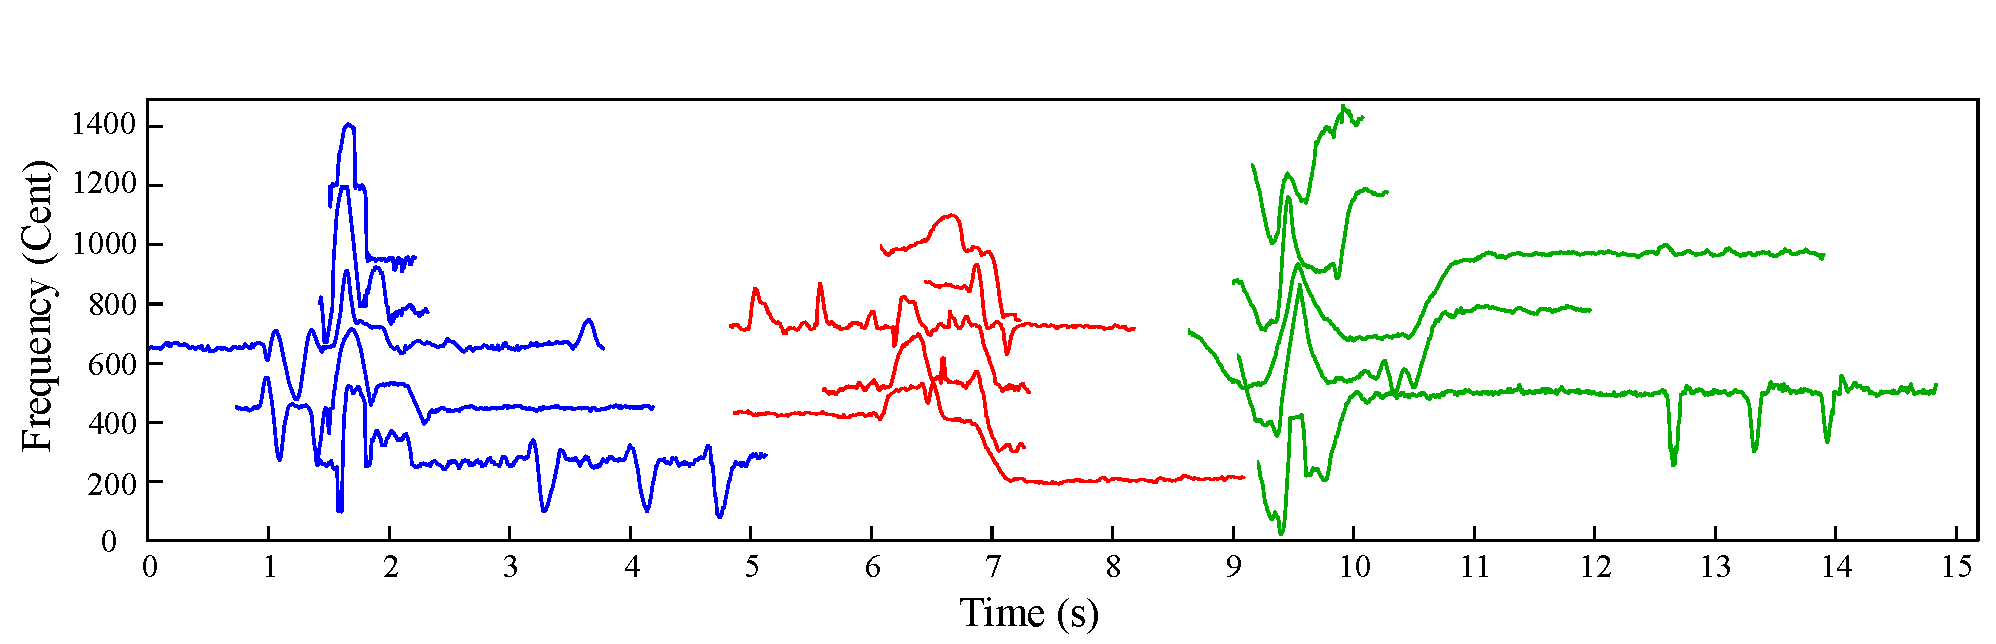
\includegraphics[width=\figSizeHundred]{ch01_introduction/figures/phraseClassesExample.pdf}
	\end{center}
	\caption{Pitch contours of occurrences of three different characteristic melodic phrases in Hindustani music. Contours are frequency transposed and time shifted for a better visualization.\TODO{diff aspect ratio?}}
	\label{fig:phraseComplexityExample_intro}
\end{figure}

An aspect that makes processing of melodies in \gls{iam} both interesting and challenging at the same time is the improvisatory nature of the music. The characteristic melodic phrases of \glspl{raga} (Section XX) act as the basis for artists to improvise, providing them with a medium to express creativity during \gls{raga} rendition. Since the essence of the music largely lies in the improvisatory aspects, artists bring in novelty through creatively transforming these melodic phrases as much as possible within the periphery defined by the \gls{raga} grammar. Therefore, the surface representation of these melodic phrases vary a lot across their occurrences. This high degree of variations in terms of the overall duration of a phrase, non-linear time warpings and the added melodic ornaments together pose a big challenge for melodic similarity computation and pattern extraction in \gls{iam}. In~\figref{phraseComplexityExample_intro} we illustrate this variability by showing the pitch contours of the different occurrences of three characteristic melodic phrases of the \gls{raga} Alaiya Bilawal. We can clearly see that the duration of a phrase across its occurrences varies a lot and the steady melodic regions are highly varied in terms of the duration and the presence of melodic ornaments. Thus, due to the improvisatory nature of the music, pattern processing in melodies of \gls{iam} becomes a challenging task. This context provides an opportunity to get deeper insights into the perception of melodic similarity and into the cultural influences on melodic similarity. 

Melodic characteristics in \gls{iam} differ significantly from a lot of other music traditions that are often the focus of studies in \gls{mir}. One peculiar characteristic of the melodies in Carnatic music (Section XX) is the meandering movement of the predominant pitch. Such melodic characteristics pose a challenge to melody transcription, a step often involved in the process of abstraction of melody. In addition, since these rapid pitch movements are characteristics aspect of melodic patterns they need to be preserved while computing melodic similarity, implying a fine grained representation of melody. Using a fine grained continuous predominant pitch representation of melody makes the task of pattern discovery further more difficult because of the computational complexity involved in the task.

%A beat level summarization of features, which is often performed in a number of tasks in \gls{MIR} to reduce the time-series dimensionality is not suited for melodies in \gls{iam}. 

%As mentioned, a composition mainly acts as a skeleton or a framework for an artist to construct a melody. In fact, typically the opening unmetered section, \gls{alap}, is not not based on any composition but is completely improvised. 

A vast majority of approaches for pattern processing in music focus on intra-opus or intra-recording pattern discovery. Since computational complexity is often one of the primary concerns in such a task, long duration of the performances in \gls{iam} pose a unique challenge. For long duration audio recordings lasting around an hour computational of self similarity becomes a computationally challenging task. To better understand the magnitude of computational complexity, consider a predominant pitch sequence of an hour long recording, sampled at 50\,Hz\footnote{a near-optimal sampling rate reported in \secref{sec:patterns_evaluation_of_similarity_measures}}. The pitch sequence comprises $1.8x10^{5}$ number of samples, which in turn amounts to nearly $3.2x10^{10}$ cells in the self similarity matrix. \XXX{S}{J}{Is this a strong point? how can we make it impressive} Thus, long performances in \gls{iam} introduce another set of challenges to this task. However, at the same time it is an opportunity as it provides a use-case to devise and test scalable approaches for pattern discovery from audio recordings. 


%Techniques that are typically employed to reduce the computational complexity in pattern processing task are; transcribe the melody to generate a symbolic score like representation and considering dimensionality reduced version of the feature, usually done through beat duration averaging. Applicability of both these techniques is questionable in the context of \gls{iam} owing the melodic characteristics. Melodic transcription is very complex and an ill defined task for melodic in \gls{iam}. And beat level summarization is musically not relevant since we are intersted in considering fine grained melodic nuances in the computation of melodic similarity. Moreover, estimation of beat locations is a  \TODO{complete it nicely}

\TODO{we are looking after really short duration patterns, that is also another challenge, please note that. Also typically beat summarization is done to reduce computational complexity, that can't be done here because 1) we wnt to present melodic nuances as the yare imp for simlarity and beat restimation is hard. Also for very small duration pattern that doesn't make sense....}


There is no standard frequency that is used as a reference for tuning instruments and voice in a music performances of \gls{iam}. The tonic pitch of the lead artist acts as the base frequency using which all the other instruments are tuned. Tonic pitch varies across artists and may vary across the different performance of an artist. In addition, an artist is free to choose any arbitrary frequency as a tonic in a performance. This aspect of music performance in \gls{iam} makes it difficult to directly compare melodies across different artists and audio recordings. 

There are many music traditions in the world where the manifestations of the seemingly transversal musical concepts such as melody and rhythm present a wide range of challenges to the current computational approaches in \gls{mir}. However, a very important factor behind selecting \gls{iam} for this analysis is the existence of musicological literature and well established music theory. \gls{iam} is an old music tradition whose origins can be traced back to the Vedas dating back to 1500 BCE. With that history, musical concepts in \gls{iam} are well studied and there exists a rich literature. This can be regarded as an opportunity, since basing the methodologies on the established music theories can speed up the advancements of computational approaches. 



%However at the same time not every computational task can directly benefit from the existing music theory. For example, the theory behind the concept of \gls{raga} in \gls{iam} elaborates WTF is happening to my mind!!!!!

%In this dissertation our focus is from an engineering perspective and solely on the computational aspects, we take established music theories for granted. Notably that is one major difference between an analysis like ours and studies in ethno-musicollogical. 


These challenges and opportunities offered by \gls{iam} sets in a unique context to develop novel methodologies for computational melodic anlaysis, and thus, improve the current state of the art in \gls{mir}. 






%
%\begin{itemize}
%	\item in general music similaity, search and discovery. Different applications and context
%	\item melodic analysis->representation of tonal content often used->melodic representaiton->difficulaty in extraction
%	\item problems which are solved by the state of the art in melody extraction for different music types
%	\item for which music types melodic anlaysis make more sense and have been done successfully.
%	\item Symbolic domain research, a lot of work.
%	\item Key detection and cover song detection.
%\end{itemize}
%
%\begin{itemize}
%	\item Music similarity focus in MIR
%	\item application and context of music similarity
%	\item how that has given rise to search and discovery in different contexts
%	\item use cases/ applications / relevant problems within similarity and search and discovery
%\end{itemize}

\section{Scope and Objectives}
\label{sec:intro_scope_context_relevance}

In this section we define the scope of our research work, clearly outline our objectives and enumerate the research questions addressed in this dissertation. 

Computational description and characterization of melodies is a broad research topic that can be approached from a number of perspectives involving different disciplines of science. In this dissertation we take a data-driven engineering approach and focus solely on the computational aspects of melodic analysis, building on top of the established music theories. Our applied research methodology, stands at an intersection of signal processing, machine learning and time-series analysis. We focus on content-based processing and the input data used in our approaches comprise audio recordings. The only exception to this is the approach described in~\secref{sec:patterns_characterization_of_melodic_patterns}, which utilize the associated editorial metadata of the recordings in addition to the audio data. The proposed approaches in this thesis are devised and evaluated on music collections in \gls{iam} that includes both Hindustani and Carnatic music. We now outline our broad objectives in this dissertation.

\begin{itemize}
%	\item To identify research tasks within computational melodic analysis that are relevant to \gls{iam}, and which can take advantage of the challenges and opportunities offered by this music tradition to improve the state of the art in \gls{mir}.
	\item To perform a critical review of the existing approaches in \gls{mir} relevant to our work in this dissertation.
	\item To build representative music corpora of \gls{iam} that comprises audio recordings and relevant editorial metadata, and use that to compile sizable and well annotated tests datasets for melodic analyses.
	\item To devise scalable pattern processing in \gls{iam}, which includes computational of melodic similarity, discovery and characterization of melodic patterns.
	\item To devise culture-aware and human interpretable approaches for automatic \gls{raga} recognition.
\end{itemize}

There are a number of research tasks within computational melodic analysis that are addressed in this dissertation, which sum up to achieve our broad objectives. Here we provide a brief description of these specific tasks, which also gives an idea about the evolution of the work done in this dissertation.

As mentioned before, tonic pitch of the lead artist in a performance is the base frequency used for tuning by other instruments. For a meaningful comparison of melodies across artists and their recordings, identification of the tonic pitch in a recording is paramount. In recent past there are a number of methods proposed for tonic identification. However, a comparative evaluation of these methods on a common set of datasets is required to reach a consensus on the best performing method. We perform an extensive comparative evaluation of seven different tonic identification methods on six diverse datasets of \gls{iam} and use the best method in our work.

Melody segmentation is a crucial step in pattern processing tasks, specifically in discovery of melodic patterns. Since \gls{nyas} \gls{svara} occurrences mark the boundaries of characteristic melodic phrases of \glspl{raga} in Hindustani music, detection of such segments becomes important for melodic segmentation. We therefore address the task of automatically segmenting \gls{nyas} \gls{svara} segments in the melodies of \gls{iam}.





\TODO{Objective of reproducible research, CompMusic philosophy}









we take an engineering perspective, MIR types approach of describing music, within and following CompMusic ideologies, culture specific in a multicultral context, applied, and micture of culture specific and 



\section{Organization and Outline of the thesis}
\label{sec:intro_organization}

\cleartorecto%!TEX root = ../thesis_a4.tex

\chapter{Literature review}
\label{sec:SOA}

\section{Introduction}

The literature review presented in this chapter is divided into two parts.
Firstly, we summarise existing work on the definition and characterisation of tagging systems.
We describe what a tagging system is, how different authors have proposed to categorize tagging systems, the motivations that users have when annotating content and the different types of tags resulting from these annotations. Additionally, we discuss problems that are typically found in tagging systems and highlight some of the solutions that are commonly proposed. 
Secondly, we focus on existing specific literature about tag recommendation systems.
We outline the different approaches that have been proposed for tag recommendation, describe how these approaches are normally evaluated, and finally summarise research about the impact that tag recommendation is expected to have on the folksonomies of tagging systems.


\section{Tagging systems}
\label{sec:SOA:tagging_systems}

Tagging systems systems have been well studied since the popularisation of tags in online sharing platforms and the social web in general.
From a broad perspective, tagging is the process of assigning tags to content resources.
Considering that this can be done manually by users or automatically by machines, tagging approaches can be divided into \emph{manual} and \emph{automatic} tagging~\citep{Wang2012}.
The focus of this thesis is on manual tagging systems.
Manual tagging systems can provide different levels of assistance during the tagging process (e.g.,~the system can suggest popular tags to the user) or provide no assistance at all, but in both cases users have the final decision on whether or not to assign a given tag to a content resource. Fig.~\ref{fig:manual_tagging_interfaces} shows the manual tagging interface of three online multimedia sharing sites.
Contrastingly, automatic tagging systems are designed to automatically add tags to resources without the need (or very little need) of human intervention. 
%Typically, these systems analyse content resources to extract low-level features, and then machine learning algorithms are trained on the basis of these features to be able to predict tags that are suitable for the resources being annotated. 
%Another common pattern for automatic tagging is the definition of a multidimensional feature space (based on the aforementioned low-level features) in which similarity measures can be defined to select content resources similar to a given target. If the similar resources have already been annotated with some tags, then these tags can be propagated to the target resource. These automatic approaches are known as model-based, and search-based automatic tagging respectively~\citep{Wang2012}. %Maybe find some references of these systems in \citep{Wang2012} section 2.2
Even though in this thesis we will not deal with automatic tagging systems, these are closely related to the tag recommendation systems that will be discussed later in this chapter, and thus we give an overview of them in Sec.~\ref{sec:soa:tag_recommendation}.


\begin{figure}[t]
  \centering
  \subbottom[]{
    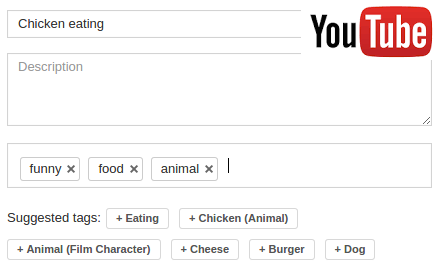
\includegraphics[width=6cm]{ch02_soa/pics/ss_youtube}}
  \hspace{0.5cm}
  \subbottom[]{
    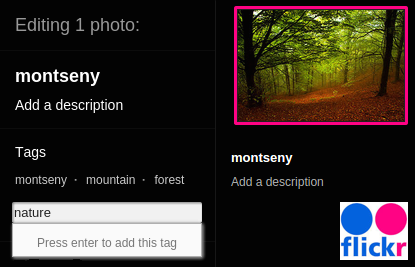
\includegraphics[width=5.65cm]{ch02_soa/pics/ss_flickr}}
  \subbottom[]{
    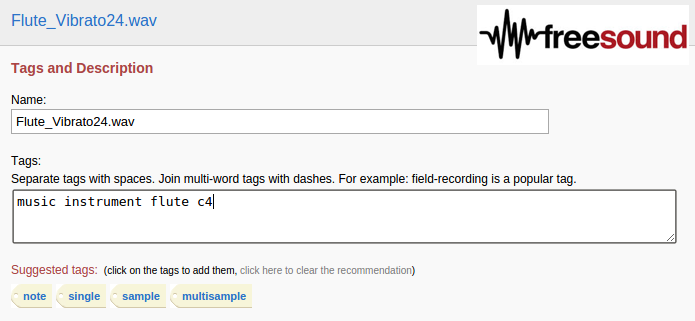
\includegraphics[width=9.47cm]{ch02_soa/pics/ss_freesound}}
  \caption[Examples of manual tagging system interfaces]{Examples of manual tagging system interfaces for (a) YouTube, (b) Flickr, and (c) Freesound. In this examples, both YouTube and Freesound annotation interfaces provide a number of suggested tags, whereas the Flickr interface does not.}
  \label{fig:manual_tagging_interfaces}
\end{figure}


In tagging systems, the individual tags that are assigned to a content resource typically represent annotations about different information dimensions or facets which, when considering the whole tagline, conform a description of the resource.
%For example, a tagline for a sound representing a recording of street ambience in Barcelona might include the following tags: \{\atag{barcelona}, \atag{street}, \atag{car}, \atag{h4n}, \atag{noisy}\}.
For example, a tagline for a sound representing a recording of the ambience in ``La Boqueria'' market in Barcelona, might include the following tags: \{\atag{coins}, \atag{barcelona}, \atag{boqueria}, \atag{atmosphere}, \atag{market}, \atag{noise}, \atag{people}\}\footnote{This example is actually taken from a sound shared in Freesound. It can be accessed in the following URL: \url{http://www.freesound.org/people/helenacm/sounds/101792/}.}.
%In that case, \atag{barcelona} indicates a specific location, \atag{street} conveys information about the generic place where the recording takes place, \atag{car} enumerats an object appearing in the recording, \atag{h4n} indicates the recording device that has been used, and \atag{noisy} describes an accoustic property of the recording.
In this case, the tags \atag{barcelona} and \atag{boqueria} indicate a specific location of the recording, \atag{market} conveys information about a generic place, \atag{people} and \atag{coins} list sound-producing elements appearing in the recording, \atag{noise} describes an acoustic property of the recording, and \atag{atmosphere} provides a possible generic classification of the type of audio. Other tags could be added, for example, to indicate the recording device used to capture the audio, or the specific time when the recording was made.
These tags are not introduced with a formal structure, and users can not indicate explicit relations among them.
The tags in the tagline, and by extension the aggregate of all distinct tags that form the folksonomy of a tagging system, are organised in a flat namespace, meaning that there is no explicit nor predefined hierarchy in which tags can be projected. 
Hence, the tagging activity is considered a categorisation process rather than a classification process, where the different tags convey information about possibly overlapping facets without formal structure~\citep{Jacob2004,halpin2006}. Conversely, formal classification systems organise items in unambiguous and exclusive concept hierarchies (or taxonomies) with a predefined and controlled vocabulary~\citep{golder2006}. %Threfore, tagging systems and their resulting folksonomies are often compared with formal classification systems and controlled vocabularies~\citep{golder2006}.
It has been argued that the use of tags instead of taxonomies with controlled vocabularies to annotate resources has two main advantages.
On the one hand, tags can better adapt to the annotation requirements of resources which might not be contemplated in controlled vocabularies. This brings a lot of flexibility as users can intuitively introduce previously non-existing tags to annotate unexpected content properties~\citep{Mathes2004,shirky2005ontology,Quintarelli2005,halpin2006,Sen,Fichter2006,Wu2006,Macgregor2004}.
On the other hand, when using tagging systems, users do not need to learn and understand the specific terms and organisation of a taxonomy, reducing the cognitive load of the annotation process and smoothing its learning curve~\citep{Quintarelli2005,shirky2005ontology,Fichter2006}. This is one of the reasons why tagging systems have become widespread in the social web and online sharing platforms in particular~\citep{Cattuto2006}.
%\citep{Cattuto2006}: ``It has been argued that the surging popularity of collaborative tagging is due to its comparatively small cognitive overhead with respect to taxonomic categorization''
However, tagging systems do exhibit significant disadvantages when compared with formal classification systems (see Sec.~\ref{soa:tagging_problems}). 


 
%%% Categorization of Tagging systems
\subsection{Types of tagging systems}
 
\cite{marlow2006} propose a categorisation for tagging systems according to seven dimensions, and discuss the implications of design choices that can be made for each dimension.
In Table~\ref{tab:tagging_systems_in_dimensions} we show some of the most popular online sharing platforms categorised according to their tagging system's characteristics and the dimensions proposed by~\cite{marlow2006}.   
The first dimension, ``tagging rights'', indicates which users of the tagging system can assign tags to resources. In some systems, only the owner of a resource can assign tags to it, while in other systems resources can be tagged by any user.
As we have seen in the introductory chapter, such a design choice leads to the emergence of either a narrow or broad folksonomy, respectively.
The second categorisation dimension, ``tagging support'', divides tagging systems according to the level of assistance given to the user during the tagging process. 
On the one hand, there are blind systems in which users are given no particular support during the tagging process. On the other hand, there are systems that feature mechanisms with different levels of complexity to suggest tags to users or guide the annotation process. Authors suggest that non-blind tagging systems reinforce the convergence of the vocabulary in the folksonomy (see Sec.~\ref{sec:soa:impact_tag_recommendation}).
The third categorisation dimension, ``aggregation model'', specifies whether the tags assigned by different users to a single resource are considered as a set of unique tags or as a union of all tags (bag of tags).
Hence, this dimension is only applicable to those tagging systems where resources can be tagged by multiple users (broad folksonomies). The different aggregation models constrain the available tagging statistics for each resource.
The fourth dimension proposed by~\cite{marlow2006} is the ``object type'', and defines the nature of the resources being tagged (e.g.,~web pages, bibliographic material, audio, video, images, etc.). The authors suggest that the type of resource has numerous implications on the resulting tags and folksonomy, hypothesising that resources without a direct textual representation (e.g.,~multimedia resources) require different kinds of annotations.
The fifth dimension, ``source of material'', separates tagging systems in those which the content to be tagged is supplied by users of the platform (typically user generated content or content from external sources like web pages), or by the platform itself. Authors suggest that the incentives that users have for tagging the content will be different depending on the source of the material.
Finally, the sixth and seventh dimensions are ``resource connectivity'' and ``social connectivity'', and indicate whether the resources or users of the system are explicitly organised in groups based on similarity, shared interests or any other aspects. \cite{marlow2006} suggest that explicit social or resource connectivity can contribute to the emergence of localised folksonomies for the defined groups, yielding particular tagging behaviours which are distinguishable from the global behaviour.
\cite{Sen} also proposed a categorisation of tagging systems that is very similar to the above described.
Although it only consists of four dimensions (``tag scope'', ``item ownership'', ``tag selection'' and ``tag sharing''), almost direct equivalences can be drawn.
%Besides Marlow's categorisation, a similar categorisation scheme for tagging systems is proposed by~\cite{Sen} which is based in four dimensions. These dimensions are very close to those proposed by~\cite{marlow2006}, and rough equivalences can be drawn: the ``tagging rights'' dimension proposed by ~\cite{marlow2006} corresponds to~\cite{Sen} ``tag scope'',  ``source of material'' by ~\cite{marlow2006} corresponds to~\cite{Sen} ``item ownership'', and finally a combination of ``tagging support'' and ``aggregation model'' dimensions find the equivalence in the ``tag selection'' and ``tag sharing'' dimensions proposed by~\cite{Sen}.
%In this thesis we mainly work with data gathered from Freesound. When analysing Freesound's tagging system characteristics with the dimensions proposed by~\cite{marlow2006} in mind, we see that Freesound features a narrow folksonomy (only the owner of a resource can annotate it) in which user-generated audio recordings are annotated. There is no explicit social connectivity among users of Freesound, but resource connectivity is sometimes present as audio recordings can be grouped into ``packs''
%Also, it worth mentioning that during the development of this thesis, a tag recommendation system was introduced in Freesound, thus altering the tagging support. 
%Furthermore, the source and type of material annotated in Freesound are user-generated audio recordings, and there is no explicit social connectivity among users of Freesound but resource connectivity is sometimes present as audio recordings can be grouped into ``packs''.
%In Table~\ref{tab:tagging_systems_in_dimensions} we show some of the most popular online sharing platforms categorised according to their tagging system's characteristics and the dimensions proposed by~\cite{marlow2006}. 
%In this thesis we mainly work with data gathered from the tagging system of Freesound. As it can be observed, Freesound features a narrow folksonomy (only the owner of a resource can annotate it) in which user-generated audio recordings are annotated. There is no explicit social connectivity among users of Freesound, but resource connectivity is sometimes present as audio recordings can be grouped into ``packs''. Furthermore, it is worth mentioning that during the development of this thesis, a tag recommendation system was introduced in Freesound. For more details on Freesound's characteristics, see Appendix~\hyperref[appendix:Freesound]{A}.


\begin{table}
\begin{threeparttable}
\centering
\ra{1.3}
\tiny
\begin{tabular}{@{}P{1.5cm}P{1.1cm}P{1.1cm}P{1.2cm}P{1.2cm}P{1.2cm}P{1.2cm}P{1.2cm}@{}}%
\toprule
%
\includegraphics[width=10cm]{ch00/pics/table_todo}
 & Flickr & YouTube & Soundcloud & Freesound & Delicious & Bibsonomy & CiteULike \\
 \midrule
\textbf{Tagging rights} & Owner & Owner & Owner & Owner & Everyone & Everyone & Everyone \\
\textbf{Tagging support} & Blind & Tag rec. & Auto-completion & Tag rec. & Tag rec. & Tag rec. & Blind \\
\textbf{Object type} & Photos & Video & Music and sounds & Sounds & Bookmarks & Biblio. ref., bookmarks & Biblio. ref. \\
\textbf{Source of material} & User-generated & User-generated & User-generated & User-generated & User-provided & User-provided, user-generated & User-provided, user-generated \\
\textbf{Resource connectivity} & Albums & Categories & Sets & Packs & - & - & - \\
\textbf{Social connectivity} & Groups, Followers & Channels, Followers & Groups, Followers & Followers & Followers & Groups & Groups, Followers \\
\bottomrule
\end{tabular}

\caption[Popular online sharing sites categorised in the dimensions defined in~\cite{marlow2006}]{Popular online sharing sites categorised in the dimensions defined in~\cite{marlow2006}. As the functionalities of some of these systems changed over time, we list here its characteristics in their state at the time of this writing. Note that the ``aggregation model'' dimension is not included in the table because it is typically not available.} 
\label{tab:tagging_systems_in_dimensions}
\end{threeparttable}
\end{table}



%%% User motivations for tagging 
\subsection{User motivations for tagging}
\label{soa:user_motivations}

\begin{table}[p]
\begin{threeparttable}
\centering
\ra{1.2}
\footnotesize
\begin{tabular}{@{}lp{9cm}@{}} \toprule
\textbf{Name} & \textbf{Description}  \\ 
\midrule 

Future Retrieval & Tags that users add to facilitate the future retrieval of the annotated resources. These tags can describe particular properties of a resource which are relevant to a broad audience and can be effectively used for indexing purposes. However, future retrieval tags can also include information which is only relevant to the user performing the annotation such as a tag like \texttt{toread}, which is typically used as a future reminder for the annotator. \\

Contribution and Sharing & These are tags that serve the purpose of categorising resources into rather common concepts and facilitate in this way future retrieval for other users of the platform. \\

Attract Attention & Some users choose to add popular tags when annotating their own resources to deliberately increase their reachability. This particular case can have a negative impact in the quality of the annotations if popular tags are chosen that have no relation with the actual content. \\

Play and Competition & Some tagging systems feature interfaces in which the annotation process is presented as an entertaining activity where users can, for instance, cooperate on annotating a resource. These systems are typically known as ``games with a purpose''~\citep{Ahn2006}. The most well known example of a game with a purpose in the tagging field is the ESP game~\citep{VonAhn2004}, in which pairs of users need to concurrently annotate a particular resource and are rewarded a number of points in accordance with their agreement in the chosen tags. \\

Self Presentation & These are tags that bear some aspect of the identity of the user that annotates a resource.~\cite{marlow2006} show, as an example of this kind of tags, the tag \texttt{seen live}, which sets a personal relation between the annotator and the resource. \\

Opinion Expression & Tags that users add with the purpose of expressing their subjective judgement or opinion about a resource. \\

Task Organisation & Similarly to some tags that could be in the future retrieval category, task organisation tags are used for organising resources through associated tasks that a particular user relates with the resource (e.g.,~\texttt{todo}, \texttt{toread}). \\

Social Signalling & Tags can be chosen to convey contextual information about a resource. For example, the name of the event in which a photo has been taken. In this case, users might be motivated by communicating their presence at that event. \\

Money & In some cases, users are being paid to annotate resources, typically through the use of platforms like the Amazon Mechanical Turk (\url{http://www.mturk.com/mturk/welcome}). \\%)$^a$. \\%\footnote{\url{http://www.mturk.com/mturk/welcome}}. \\

Technological Ease & Users can be also motivated by the ease of use of tagging systems (and sharing platforms in general) to annotate resources, so that the easier the tagging process is, the more likely users will be to annotate resources. \\
\bottomrule
\end{tabular}
\caption[Potential tagging motivations listed by~\cite{Gupta2010}]{Potential tagging motivations listed by~\cite{Gupta2010}.}
\label{tab:tagging_motivations}
%\begin{tablenotes}
%    \item[a] \url{http://www.mturk.com/mturk/welcome}.
%\end{tablenotes}
\end{threeparttable}
\end{table}

Several authors have studied the motivations or incentives that users have when tagging online resources~\citep{Mathes2004,marlow2006,golder2006,Sen,Xu2006,Ames2007,Gupta2010}.
\cite{marlow2006} propose a high-level categorisation of potential user motivations in two categories: ``organisational'' and ``social''. 
The ``organisational'' category includes tagging activities motivated by the aim of bringing a particular structure and organisation to contributed resources. In this case, users might develop particular tagging patterns and also adopt common patterns observed in other users of the tagging system. Tags under the ``organisational'' category should, in general, ease the future retrieval of the resources being tagged.
Tagging activities under the ``social'' category include the listing of user opinions and other communicative aspects that allow users to express themselves.
Besides these two broad categories,~\cite{marlow2006} also describe several more specific potential motivations for tagging resources.~\cite{Gupta2010} summarise these more specific categories along with others found in the literature~\citep{Mathes2004,golder2006,Xu2006,Sen,Ames2007}, and finally enumerate ten specific and non-exclusive categories which exemplify possible user motivations for tagging resources. Table~\ref{tab:tagging_motivations} lists these categories and provides a brief explanation for each one.
%These different motivations are tightly coupled with different kinds of tags that result of the annotation process~\cite{marlow2006}. That point is discussed below on Sec.~\ref{soa:types_of_tags}.

Besides these categorisations, of particular interest is the work by~\cite{Ames2007}, in which an empirical tagging study is carried out with participants being interviewed about their motivations when tagging pictures to be uploaded to Flickr.
In this study, the authors classify the responses provided by the interviewed participants in similar categories as those listed in Table~\ref{tab:tagging_motivations}. The observed motivations are, basically, those related to expressing user's opinions or relation with the photos to other known users of the system such as family or friends (roughly corresponding to ``self presentation'', ``opinion expression'' and ``social signalling'' categories of Table~\ref{tab:tagging_motivations}). Moreover, motivations related to the organisation of the resources (for easing future retrieval to both the owners of the photos and to other users of the system) are also repeatedly reported. Of particular relevance is the fact that, according to the interviews, participants are not aware of all potential motivations and benefits of tagging systems when annotating resources, and the decisions of which tags to choose are taken in an intuitive way rather than in an informed fashion. In relation to this, in a study by~\cite{marlow2006}, also with Flickr tagging data, authors suggest that the more resources a user has tagged, the more aware the user is about the relevance of chosen tags and annotation quality. In other words, as users learn to tag, their motivations change.




\subsection{Types of tags}
\label{soa:types_of_tags}


\begin{sidewaystable}
\begin{threeparttable}
\centering
\ra{3.0}
\footnotesize
\begin{tabular}{P{2.2cm}:L{1.8cm}:L{1.8cm}:L{1.8cm}:L{1.8cm}:L{1.8cm}:L{2.2cm}:L{1.8cm}:L{1.8cm}}
\toprule
\multicolumn{9}{l}{} \\[-1.05cm]
\textbf{\cite{Sen}} & \multicolumn{5}{c:}{Factual\tnote{a}} & Subjective & \multicolumn{2}{c}{Personal\tnote{a}} \\ %\hline
\textbf{\cite{cantador2010}} & \multicolumn{3}{c:}{Content-based} & \multicolumn{2}{c:}{Context-based} & Subjective & \multicolumn{2}{c}{Organisational} \\ %\hline
\textbf{\cite{Xu2006}} & Content-based & \multicolumn{2}{c:}{Attribute} & \multicolumn{2}{c:}{Context-based} & Subjective & \multicolumn{2}{c}{Organisational} \\ %\hline
\textbf{\cite{golder2006}} & What or who it is about & What is & Who owns it & \multicolumn{2}{c:}{Refining other categories} & Identifying qualities or characteristics & Task organisation & Self reference \\ %\hline
\textbf{\cite{Bischoff2008}} & Topic & Type & Author or owner & Time & Location & Opinions and qualities & Usage context & Self reference \\ %\hline
\textbf{\cite{Gupta2010}} & Content-based & Attribute & Ownership & \multicolumn{2}{c:}{Context} & Qualities and characteristics & Or\-ga\-ni\-sa\-tio\-nal and Purpose & Self reference\\
\multicolumn{9}{l}{} \\[-0.85cm]

\bottomrule
\end{tabular}

\begin{tablenotes}
    \item[a] These categories are also listed in \cite{Gupta2010}.
\end{tablenotes}

\caption[Types of tags, adapted and extended from the works of~\cite{cantador2010} and~\cite{Bischoff2008}]{Types of tags according to the kind of information conveyed about resources. This table is adapted and extended from the works of~\cite{cantador2010} and~\cite{Bischoff2008}.}
\label{tab:tag_types}
\end{threeparttable}
\end{sidewaystable}

In the previous section we have seen how some authors categorise tags in terms of potential user motivations or incentives. 
Another dimension in which tags can be categorised is on the basis of the kind of information that these convey about resources.
In that direction, several authors have proposed different, but highly related categorisations which are summarised in Table~\ref{tab:tag_types} and which are generic enough to be applied in tagging systems of different domains~\citep{golder2006,Sen,Xu2006,Bischoff2008,Gupta2010,cantador2010}. 
Among these categorisations featuring broader tag categories (upper rows in Table~\ref{tab:tag_types}), we find particularly meaningful the four-class categorisation proposed by~\cite{cantador2010}. Tags under ``content-based'' category describe the objects and qualities of a resource (e.g.,~content-based tags might enumerate the musical instruments that are present in an audio resource or its music genre). Tags under ``context-based'' category provide information about the context in which the resource was created (e.g.,~the location where a photo was taken or the time of the year in which a video was recorded). ``Subjective'' tags are those which express personal opinions that the tagger has about a resource at hand, such as quality judgements or mood annotations. Finally, ``organisational'' tags annotate resources with information that is, a priori, only useful for the annotator of the resource such as reminders related to the resource or self-referencing comments.
As can be seen in Table~\ref{tab:tag_types}, the other proposed broad categorisations are very similar~\citep{Sen,Xu2006}. Contrastingly, categorisations proposed by~\cite{golder2006}, \cite{Bischoff2008}, and \cite{Gupta2010}, include more fine-grained categories that can be easily understood as subdivisions of those broader categories mentioned above. 

Empirical research on the categorisation of tags has also been performed. \cite{Simons2008} analyses the Flickr tagcloud and performs a manual classification of the tags into a list of categories crafted to fit the data. By mapping these tailored categories to the broader categories proposed by~\cite{cantador2010}, it can be seen that around 66\% of tags belong to either ``content-based'' or ``context-based'' categories. The remaining 33\% can be classified as ``subjective'' or ``organisational'' tags. 
Similarly,~\cite{Bischoff2008} perform an analysis on the distribution of tags among their proposed categories using data from Delicious, Last.fm and Flickr. After a manual classification of a sample of all used tags, 55\% of the tags belong to either ``topic'', ``type'' or ``location'' categories, which are related to the broader ``content-based'' and ``context-based'' categories defined by~\cite{cantador2010}.
Furthermore, \cite{cantador2010} propose a rule-based method for automatically classifying tags into their proposed four broad categories. The method is based on the use of natural language processing techniques and YAGO\footnote{\url{http://www.mpi-inf.mpg.de/departments/databases-and-information-systems/research/yago-naga/yago/}.}, an external knowledge base. By performing a part-of-speech analysis of the tags and matching them to concepts of the YAGO knowledge base, the authors are able to determine to which category a tag belongs. Using data collected from Flickr, the authors performed the classification and found that, among those tags whose category could be predicted, 64\% are considered to be either ``content-based'' or ``context-based'' tags, while the others belong to ``subjective'' or ``organisational'' categories. As can be observed, these results are consistent with those reported by~\cite{Simons2008} and~\cite{Bischoff2008}.

By comparing Tables~\ref{tab:tagging_motivations} and~\ref{tab:tag_types}, it can be easily seen that tag types and tagging motivations are tightly coupled.
We explained before in Sec.~\ref{tab:tagging_motivations} that~\cite{Ames2007} found that users are more motivated for introducing tags expressing subjective opinions and self-references than to introduce tags describing the nature of the resources for their organisation. Considering this observation, we would expect to find more tags corresponding to the ``subjective'' and ``organisational'' categories rather than to the ``content-based'' and ``context-based'' categories, which is not what has been observed by~\cite{Simons2008},~\cite{Bischoff2008}, and~\cite{cantador2010}.
Interestingly, among the resulting types of tags and motivations, not all of them are equally suitable for generating useful metadata for indexing the content of online sharing platforms. In the case of systems featuring narrow folksonomies such as Flickr or Freesound, those tags that convey information which is meaningful not only to the owners of a resource but also to the other users of the platform, are crucial in order to successfully index content. Thus, according to the categorisation proposed by~\cite{cantador2010}, the presence of ``content-based'' and ``context-based'' tags is more desirable than ``subjective'' and ``organisational'' tag types. Conversely, in broad folksonomies such as Declious or Last.fm, ``subjective'' and ``organisational'' tags can be as important as ``content-based'' and ``context-based''. This is because in these systems users mainly tag for their self-organisation, and the used tagging conventions do not necessarily need to be meaningful to other users of the platform~\citep{DeMeo2013}.


%%% Problems of tagging systems
\subsection{Tagging systems' problems and solutions}
\label{soa:tagging_problems}

We have seen that the flexibility provided by tagging systems typically carries a number of well known problems which limit the possibilities of indexing, searching and browsing in sharing platforms~\citep{golder2006,halpin2006,Guy2006}. A very common problem is the presence of tags with typographical errors and tags formed with several concatenated words.~\cite{Guy2006} found that 40\% of Flickr tags and 28\% of Delicious tags contain misspellings or compound words that could not be mapped into a dictionary. These tags become less relevant, as a tagging system most probably treats misspelled versions of words as different tags. Moreover, word concatenation easily leads to different variations of a single concept.
In addition to that, it is very common that a single tag might have several different meanings (polysemy), and thus some users might employ it thinking of one meaning and some other users might employ it thinking of another meaning. Without a successful method for disambiguation, this results in making relations between resources which are semantically not meaningful. For example, search results might display resources related to different meanings of the query terms. Conversely, it is also quite common that several tags refer to a single concept (synonymy) and users employ them indistinctly. In that case, some relevant resources might be left out of the results of a query because systems are not generally aware of synonymy relations. Polysemy and synonymy problems have been empirically evaluated by~\cite{Spiteri2006}, analysing data of folksonomies gathered from Delicious, Furl and Technorati\footnote{Furl is a no longer existing online sharing platform. In it, users shared web bookmarks (similarly to Delicious). Technorati is currently a publisher advertising platform, but used to be a blog tracking site (\url{http://www.technorati.com/}).}, where it was found that between 12\% and 22\% of the tags potentially feature these kind of problems.

Another common problem of tagging systems is the use of tags that are only relevant for a specific user or the use of tagging conventions which are only known by particular users. These kind of tags convey information which is not generally useful to the community, and therefore their organisational value is limited. For example, a user might annotate resources using very particular tags whose meaning is not known to other users, and these annotations might appear to be totally unrelated to the resources.~\cite{Kennedy2006a} found that, given a Flickr image, only 50\% of the tags can actually be easily related to the content of the image or even to the image at all.
That can particularly become a problem in tagging systems with narrow folksonomies, in which tags that have a shared meaning for the community should be reinforced to improve indexing, searching and browsing possibilities~\citep{Guy2006}. 
Furthermore, a typical problem of tagging systems is the \emph{lack of tags}. Some studies show that user provided tags tend to be incomplete. As an example,~\cite{Sigurbjornsson2008} show that 50\% of images in Flickr have less than four tags, and~\cite{Zhao2010} show that YouTtube videos have an average of five tags, which means that annotations are not very comprehensive.

On an even higher level, different tagging styles can also create a problem for the tagging system if there are no signs of consensus.
If a common vocabulary is not shared among users, the informational value of tags is lessened and resources become less reachable (see Sec.~\ref{sec:soa:impact_tag_recommendation}). Furthermore, the co-existence of different languages in a single tagging system can also become an obvious problem~\citep{halpin2006}.
Overall, most of these issues are inherent to the vocabulary problem~\citep{Furnas1987}, caused by the lack of well defined tagging guidelines and the different rationales that users can apply during the tagging process. Nevertheless, the design and functionalities of tagging systems potentially have a big influence on the tagging behaviour when annotating resources, and this could be shaped so that typical tagging problems can be lessened~\citep{Wang2012}.

% on another level: specificity of the tags in relation to the content (eg. an hour of video, where the tag applies?). (Relate cost of tagging with batch tagging functionality in Flickr (\citep{Wang2012}), an tagging quality with tagging of specific regions in images or subclips in videos (mention that idea applies to soundcloud sets) tagging studies (search references in \citep{Wang2012}, annotation B).)

% The Structure and Form of Folksonomy Tags: The Road to the Public Library Catalog
%\citep{Spiteri2006}: analyse a month of data from delicious, furl (bookmark sharing) and technorati (blog sharing) and compare the emerging folksonomy with National information Standards Organization (NISO) guidelines for constructing controlled vocabularies.
%- most of the tags $\approx$95\% are nouns instead of adjectives and adverbs, which fits NISO recommendations
%- problems arise with inconsistent use of plural forms and ambiguous tags (compared to NISO recommendations), and that could be improved during the annotation phase

In order to mitigate some of the above mentioned tagging systems' problems, many authors have focused on approaches in which manual tagging is combined with computer algorithms to try to ``optimise'' the taglines introduced by users. Some of these approaches are meant to be used at the time when users annotate newly uploaded resources, but others are focused on improving already existing annotations.
\cite{Wang2012} introduce the concept of \emph{assistive tagging} to refer to these approaches, and propose a classification into three groups. 
The first group, ``tagging with data selection and organisation'', includes these approaches in which tagging systems automatically detect already existing resources which are poorly described and ask users to annotate them. In this case, many users can contribute to improving the annotations of a pool of selected resources, and the system can prioritise which content should be annotated first~\citep{Huang2008,Wang2011a}. % and optimise, for example, the implicit creation of training sets for machine learning algorithms that can later be used to automatically annotate other unlabelled resources~\citep{Huang2008,Wang2011a}.
A similar idea consists of the organisation of data to be annotated in clusters, which then become the smallest unit of tagging. Tags assigned to particular clusters are propagated to all resources of that cluster. This approach has been mainly applied in photo tagging, with clusters formed on the basis of face recognition algorithms~\citep{Suh2004,Cui2007,Tian2007}, or on the basis of sub regions of an image~\citep{Tang2010}. In the latter case, it is interesting that by clustering photos according to smaller regions and then annotating the regions, the tags can be applied to many photos at once. 
These methods are oriented to batch tagging of resources which, in the context of an online sharing site, does not necessarily need to be performed at upload time by the authors of the content. Instead, it can be performed in a collaborative fashion by other users of the platform.

The second group of assistive tagging strategies, ``tag processing'', includes those approaches in which existing annotated resources are post-processed in order to automatically correct or refine the descriptions. For example, in photo tagging systems, images can be segmented and machine learning algorithms can be trained to learn the mapping of introduced tags with particular regions, and then propagate the tags to other images with similar regions~\citep{Liu2010b,Feng2010,Liu2011}. Similar ideas, applied at a temporal level rather than at the region level, have been applied to video tagging~\citep{Ulges2008}. Furthermore, systems can be trained to compute a relevance score for the tags assigned to a resource based on the analysis of its content, and filter in this way tags with low scores~\citep{Liu2009,Li2009,Chen2010a,Fan2010}.
Another approach for post-processing user provided annotations is the use of knowledge bases like WordNet~\citep{Miller1995} to extend annotations with synonyms and hypernyms or filter out tags which are unrelated according to the knowledge base~\citep{Liu2010a}. % approach with topic modeling \cite{Xu2009} and matrix decomposition \cite{Zhu2010a}
Finally, the third group of assistive tagging strategies identified by~\cite{Wang2012}, ``tag recommendation'', consists of approaches in which tagging systems suggest tags to users during the annotation process, thus potentially shaping users' tagging behaviour. These systems are the main topic of the present thesis, and are discussed in the following section.



%%% Tag recommendation

\section{Tag recommendation}
\label{sec:soa:tag_recommendation}

The existing literature on tag recommendation systems is generally focused on recommendation systems for image or social bookmarking sharing sites.
However, highly related to tag recommendation systems are automatic tagging systems.
In essence, automatic tagging systems and tag recommendation systems share their main goal: generating a set of relevant tags for a given resource.
Hence, a lot of the techniques described in the literature are applicable to the two kinds of systems.
In this section, we summarise a number of approaches that, either being more focused on tag recommendation or automatic tagging, are of relevance to contextualise the work described in this thesis. Nevertheless, we put our focus on the systems designed for the task of tag recommendation.

Tag recommendation systems can be classified according to the main source of information that is used in the recommendation process.
In general, approaches can be separated in \emph{i)} systems based on the content analysis of the resources, \emph{ii)} systems based on the folksonomy of a tagging system, and \emph{iii)} systems based on contextual data~\citep{Wang2012}. 
In the following sections, we review existing literature on each one of these approaches.
Table~\ref{tab:soa_methods_comparisson} shows a summary of all approaches reviewed in these sections.


\begin{sidewaystable}
\begin{threeparttable}
\centering
\ra{1.1} %0.2
\tiny
\begin{tabular}{@{}p{3.0cm}p{1.35cm}P{2.3cm}P{1.6cm}P{2.3cm}p{1.6cm}p{1.45cm}T{1.0cm}p{2.5cm}@{}}
% HEADER
\toprule
& \textbf{Focus} & \textbf{Type of resource} & \textbf{Type of approach} & \textbf{Based on} & \textbf{Sharing platform} & \textbf{Evaluation method} & \textbf{Dataset size} & \textbf{Evaluation} \hspace{0.5cm} \textbf{measures} \\
\midrule
% ROWS
\cite{Barnard2003} & Auto Tag. & Image & CO & IF, MOD & - & Prediction & 9,000 & Increase of $\precision$ \\
\cite{barrington2007} & Auto Tag. & Sound & CO & AF, MOD & - & Search & 1,305 & $\precision$, $\recall$, $\fmeasure$ \\
\cite{jaske2007} & Tag. rec. & Bookmarks, Music & FO & CF, FK, PE & Bibsonomy, Delicious, Last.fm & Prediction & 361 74,854 1,853 & $\precision$, $\recall$, $\fmeasure$ \\
\cite{Sood2007} & Tag. rec. & Blog posts & CT & TF, SIM & Technorati & User assess. Prediction & 225 & $\precision$, $\recall$, $\fmeasure$ \\
\cite{Anderson2008} & Tag. rec. & Image & FO, CO & CC, IF, MOD & Flickr & Prediction & 924 & $MRR$, $S$, $P$ \\
\cite{Chen2008a} & Tag. rec. & Image & CO & IF, MOD & Flickr & User assess. & 930 & \tnote{a} \\
\cite{Garg2008} & Tag. rec. & Image & FO & CC, PE & Flickr & Prediction & 50M & $MRR$, $S$, $P$ \\
\cite{Li2006} & Auto Tag. & Image & CO & IF, MOD & Flickr & User assess. Prediction & 5,411 47,000 & $\precision$, $\recall$, $\fmeasure$, $S$ \\
\cite{Lipczak2008} & Tag. rec. & Bookmarks & FO & CC, PE & Bibsonomy & Prediction & 274,139 & $\precision$, $\recall$, $\fmeasure$ \\
\cite{Naaman2008} & Tag. rec. & Image & CT & GPS & Flickr & Prototype & 100,000 & \tnote{b} \\
\cite{Sigurbjornsson2008} & Tag. rec. & Image & FO & CC & Flickr & User assess. & 331 & $MRR$, $S$, $P$ \\
\cite{Song2008} & Tag. rec. & Bookmarks & FO & CC, TCL & Bibsonomy & Prediction & 32,279 & $\precision$, $\recall$, $\fmeasure$ \\
\cite{turnbull2008} & Auto Tag. & Music & CO & AF, MOD & - & Prediction & 500 & $\precision$, $\recall$, $\fmeasure$ \\
\cite{Cao2009} & Tag. rec. & Bookmarks & FO & CC, PE & Bibsonomy & Prediction & 274,139 378,378 & $\precision$, $\recall$, $\fmeasure$ \\
\cite{meo2009} & Tag. rec. & Bookmarks & FO & CC & Delicious & User assess. & 160 & $\precision$, $\recall$, $\fmeasure$ \\
\cite{Marinho2009} & Tag. rec. & Bookmarks & FO & PR, PE & Bibsonomy & Prediction & 378,378 & $\precision$, $\recall$, $\fmeasure$ \\
\cite{martinez2009} & Auto Tag. & Sound & CO & AF, SIM & Freesound & User assess. & 260 & \tnote{a} \\
\cite{Rendle2009} & Tag. rec. & Bookmarks & FO & PR, PE & Bibsonomy & Prediction & - & $\precision$, $\recall$, $\fmeasure$ \\
\cite{Wu2009} & Tag. rec. & Image & FO, CO & CC, IF, MOD & Flickr & User assess. & 500 & Variant of $\recall$ \\
\cite{Zhang2009} & Tag. rec. & Bookmarks & FO, CO & CC, SIM & Bibsonomy & Prediction & 464,930 & $\precision$, $\recall$, $\fmeasure$ \\
\cite{Ballan2010} & Tag. rec. & Video & FO, CO, CT & CC, IF, SIM & YouTube & User assess. & 56 & $P$ \\
\cite{Chen2010} & Tag. rec. & Video & CT & PK & YouTube & - & - & - \\
\cite{ivanov2010} & Tag. rec. & Image & CO & IF, SIM & Flickr, Goolge & Prediction & 3,200 & $\precision$, $\recall$, $\fmeasure$ \\
\cite{Lee2010} & Tag. rec. & Image & FO, CO & IF, SIM, PR & Flickr & Prediction & 25,000 & Variant of $S@\nRecommendedTagsInEvaluation$ \\
\cite{Liu2010a} & Auto Tag. & Image & FO, CO, CT & CC, IF, SIM & Flickr & User assess. & 50,000 & $\precision$, $\recall$, $\fmeasure$ \\
\cite{Rae2010} & Tag. rec. & Image & FO & CC, PR & Flickr & Prediction & 3,000 & $MRR$, $MAP$, $P@5$ \\
\cite{Sevil2010a} & Tag. rec. & Image & FO, CO & IF, SIM & Flickr & Prediction & 15,000 & $P@8$, $P@20$, $P@25$ \\
\cite{Toderici2010} & Tag. rec. & Video & CO & IF, VF, AF, MOD & YouTube & User assess. & 500 & $P$ \\
\cite{Lops2012} & Tag. rec. & Bookmarks & FO, CO & TF, SIM & Bibsonomy & Prediction & 378,378 & $\precision$, $\recall$, $\fmeasure$ \\
\cite{moha2012} & Auto Tag. & Music & CO & SIM & - & Prediction & 8,790 & $\precision$, $\recall$, $\fmeasure$ \\
%\cite{Font2013} & Tag. rec. & Sound, Image & FO & CC & Freesound, Flickr & Prediction & 118629, 107617 & $\precision$, $\recall$, $\fmeasure$ \\
%\cite{Font2014} & Tag. rec. & Sound & FO & CC, PR & Freesound & Prototype, Prediction & 140622 & \tnote{c} \\
\bottomrule
\end{tabular}
\begin{tablenotes}
    \item[a] Average over user judgement scores or agreement on judgement scores.
    \item[b] Percentage of taglines that contain at least one recommended tag. 
    %\item[c] Number of accepted tags and $\precision$, $\recall$, $\fmeasure$. 
    \vspace{0.20cm}
    \item[] ABBREVIATIONS: FO=folksonomy-based; CO=content-based; CT=context-based sources; IF=image features; AF=audio features; TF=text features; CC=tag co-occurrence in resources; PR=probabilistic model; CF=collaborative filtering; PK=PageRank algorithm; FK=FolkRank algorithm; SIM=resource similarity tag propagation; MOD=model-based tag prediction; GPS=geolocation data.
\end{tablenotes}
\caption[Summary of existing tag recommendation approaches]{Summary of tag recommendation and related auto tagging methods proposed in the literature. Entries in the table are sorted chronologically. For details on evaluation measures see Sec.~\ref{sec:soa:evluation_of_tag_recommendation}.}
\label{tab:soa_methods_comparisson}
\end{threeparttable}
\end{sidewaystable}


\subsection{Based on content analysis}
\label{sec:soa:tag_recommendation_content_analysis}

%These automatic approaches are known as model-based, and search-based automatic tagging respectively~\citep{Wang2012}. %Maybe find some references of these systems in \citep{Wang2012} section 2.2
Content-based tag recommendation systems take advantage of the analysis of the content of resources in order to provide a set of recommended tags.
For example, given an image, a content-based tag recommendation system leverages the pixel data to extract features like colour, texture and shape that can be used to derive a set of potentially relevant tags.
These approaches are marked with the abbreviation ``CO'' in the ``type of approach'' column of Table~\ref{tab:soa_methods_comparisson}.
One way in which relevant tags can be recommended after the extraction of low-level features is the use of machine learning techniques to build a model for every potential tag to be recommended. This typically implies to learn the joint probabilities between content features and the presence of particular tags (marked with the abbreviation ``MOD'' in the ``based on'' column of Table~\ref{tab:soa_methods_comparisson}). 
For that, we require of a training set with examples of resources for each tag that has to be modelled. Using these examples, a machine learning algorithm can learn the relations between low-level features and tags. Thus, given a new resource, the algorithm can predict whether a particular tag is potentially relevant. Examples of this approach have been proposed for recommending tags for image resources \citep{Barnard2003,Li2006,Anderson2008,Chen2008a,Wu2009}, audio resources \citep{barrington2007,turnbull2008}, and video resources \citep{Toderici2010}. 

The other common approach in content-based tag recommendation systems is the propagation of tags from resources that have already been annotated to resources that have not yet been annotated (marked with the abbreviation ``SIM'' in Table~\ref{tab:soa_methods_comparisson}). In this case, the extracted low-level features define a multi-dimensional feature space in which similarity measures can be defined. Then, given a resource, other similar resources can be retrieved. Hence, in these systems, tags can be propagated among similar resources. Examples of such content-based tag recommendation systems can be found in the image~\citep{Liu2010a,ivanov2010,Lee2010,Sevil2010a}, audio~\citep{martinez2009,moha2012}, video~\citep{Ballan2010}, and bookmark domains~\citep{Zhang2009,Lops2012}.

The main advantage of tag recommendation systems based on content analysis is that, after the training step, these can be applied to any resource, even if there is no associated metadata.
Conversely, a disadvantage is that these systems are not directly generalisable to other domains because the feature extraction and similarity definition steps are highly dependent on the type of resources for which tags are recommended. 
Similarly, even when staying in the same domain, content-based systems do not always generalise to resources which are sufficiently different from those used in the training step.
For instance, a system that learns to recommend tags for music resources and that is trained with a dataset of electronic music, will not necessarily perform well when tested on a dataset of classical music.
Moreover, the content analysis and training steps of content-based systems are, in general, computationally expensive, particularly if a model needs to be built for every potentially suggested tag.
Finally, in many cases, the training step of content-based models requires great human effort in building and validating the datasets from which the models will be learnt.


\subsection{Based on folksonomy analysis}
\label{sec:soa:tag_recommendation_folkosnomy_analysis}

An important number of works on tag recommendation systems are based on analysing the folksonomy of a tagging system in order to provide recommendations given a resource and a number of already existing tags assigned to that resource (i.e.,~the input tags).
As opposed to content-based systems, folksonomy-based systems are easily generalisable to several domains because the content of the resources is not analysed. However, in order to provide recommendations for a given resource, folksonomy-based systems require the presence of some already assigned tags.

To formally define a folksonomy, the adoption of the tripartite graph model proposed by~\cite{Mika2007a} is very common. This model is very similar to previous models proposed by~\cite{hoto2006} and~\cite{jaske2007}.
In Mika's model, the folksonomy is represented as a tripartite graph in which users, tags and resources are included as nodes, and edges establish ternary relations among them, the so called tag applications (Sec.~\ref{sec:intro_tagging_systems_and_folksonomies}).
The tripartite graph can be unfolded into a bipartite graph after discarding one of the three sets of nodes (i.e.,~users, tags or resources). In this way, it is possible to obtain a graph which relates tags and users, a graph which relates users and resources, and a graph which relates tags and resources. This last bipartite graph is the view of the folksonomy that we work with in this thesis, as it allows the derivation of relations between tags on the basis of their shared resources and vice versa.
Details on the formal definition of the model can be found in Chapter~\ref{sec:general} of this thesis (Sec.~\ref{sec:general:method}).
The graph that relates users and resources is not exploited in this thesis because it does not bring any particular information about tags. Furthermore, the graph that relates tags and users is neither used in this thesis because the tag recommendation systems we propose are not personalised to users' particular tagging styles (see below).
%Mika's model considers three finite sets of objects $\mathbf{A}$, $\mathbf{C}$ and $\mathbf{I}$ which correspond to ``actors'' (i.e.,~users), ``concepts'' (i.e.,~tags) and ``instances'' (i.e.,~resources). In this thesis, instead of the variables $\mathbf{A}$, $\mathbf{C}$ and $\mathbf{I}$ defined by ~\cite{Mika2007a}, we employ the notation $\users$, $\tags$ and $\resources$ respectively, which more closely relates to the ``users'', ``tags'' and ``resources'' terminology that we use.
%The sets of users, tags and resources are represented as nodes in the graph such that nodes $\vertices=\users\cup \tags\cup \resources$. The ternary relations between a user, a tag and a resource (i.e.,~tag applications) are then represented as the edges of the graph $\edges=\{\{\user,\tag,\resource\}| (\user,\tag,\resource)$ $\in \folksonomy\}$. Hence, the graph $\graph$ that represents a folksonomy $\folksonomy$ is finally defined as $\graph(\folksonomy)=\left\langle \vertices,\edges \right\rangle$. 
%The tripartite graph can be unfolded into a bipartite graph after discarding one of the three sets of nodes (i.e.,~$\users$, $\tags$ or $\resources$). In this way, it is possible to obtain the graph $\bipartiteGraphTagsUsers$ which relates tags and users, the graph $\bipartiteGraphUsersResources$ which relates users and resources, and the graph $\bipartiteGraphTagsResources$ which relates tags and resources. That last bipartite graph is the view of the folksonomy that we work with in this thesis, as it allows to derive relations between tags on the basis of their shared resources and vice versa.

Most of the tag recommendation methods based on folksonomy analysis take advantage of the co-occurrence of tags in resources in order to estimate a similarity or relatedness measure between pairs of tags\footnote{The words ``similar'' and ``related'' have, in fact, different meanings. Two tags can be considered similar if there is a considerable overlap in their meanings, or can be considered related if they convey complementary information. When talking about tags, in this thesis we use the term ``similar'' in a broad sense, referring to any sort of potentially relevant relation between tags.} (these methods are marked with the abbreviation ``CC'' in the ``based on'' column of Table~\ref{tab:soa_methods_comparisson}).
The general assumption is that tags that tend to appear together in the taglines of annotated resources are potentially similar. Using the bipartite graph relating tags and resources, it is thus possible to define a tag-tag similarity matrix in which every element indicates the number of resources in which two tags co-occur (i.e.,~the number of resources in which two tags appear together).
By applying a normalisation to this matrix, several similarity measures can be obtained, such as the widely adopted cosine similarity or the Jaccard index~\citep{Mika2007a,Markines2009}. For more details on the construction of this similarity matrix and the normalisation process we again refer the reader to Chapter~\ref{sec:general} of this thesis (Sec.~\ref{sec:general:step1}).

Given a tag-tag similarity matrix, it is possible to retrieve a ranked list of the most similar tags to a given target tag.
This is the basis of many folksonomy-based tag recommendation systems. Considering a set of input tags, potentially relevant tags can be obtained by retrieving the most similar tags to each input tag. %These potentially relevant tags are normally known as the candidate tags.
Then, these tags are aggregated into a single ranked list of candidate tags by taking into account the similarity scores with their respective input tag~\citep{Sigurbjornsson2008}. 
In general, the top tags of the aggregated set of candidates are selected to generate the output of the tag recommendation system.
Tag recommendation systems based on this approach have been proposed for the image~\citep{Anderson2008,Sigurbjornsson2008,Garg2008,Wu2009,Liu2010a,Rae2010}, video~\citep{Ballan2010}, and bookmark domains~\citep{Lipczak2008,Song2008,Cao2009,meo2009,Zhang2009}.
Both aggregation and selection procedures are applicable not only to folksonomy-based tag recommendation systems but also to those content-based systems based on tag propagation from similar resources.

%\cite{Anderson2008} & Tag. rec. & Image & FO, CO & CC, IF, MO & Flickr & Prediction & 924 & $MRR$, $S@\kappa$, $P@\kappa$ \\
%\cite{Garg2008} & Tag. rec. & Image & FO & CC & Flickr & Prediction & 50M & $MRR$, $S@\kappa$, $P@\kappa$ \\
%\cite{Sigurbjornsson2008} & Tag. rec. & Image & FO & CC & Flickr & User assessment & 331 & $MRR$, $S@\kappa$, $P@\kappa$ \\
%\cite{Wu2009} & Tag. rec. & Image & FO, CO & CC, IF, MO & Flickr & User assessment & 1M, 500 & $^f$ \\
%\cite{Liu2010a} & Auto T. & Image & FO, CO, EX & CC, IF, SIM & Flickr & User assessment & 50000 & $\precision$, $\recall$, $\fmeasure$$@\kappa$ \\
%\cite{Rae2010} & Tag. rec. & Image & FO & CC, PR & Flickr & Prediction & 3000 & $MRR$, $MAP$, $P@5$ \\
%\cite{Ballan2010} & Tag. rec. & Video & FO, CO, EX & CC, IF, SIM & Youtube & User assessment & 56 & $P@\kappa$ \\
%\cite{Lipczak2008} & Tag. rec. & Bookmarks & FO & CC & Bibsonomy & Prediction & 274139 & $\precision$, $\recall$, $\fmeasure$ \\
%\cite{Song2008} & Tag. rec. & Bookmarks & FO & CC, TCL & Bibsonomy & Prediction & 32279 & $\precision$, $\recall$, $\fmeasure$ \\
%\cite{Cao2009} & Tag. rec. & Bookmarks & FO & CC, PR & Bibsonomy & Prediction & 274139, 378378 & $\precision$, $\recall$, $\fmeasure$ \\
%\cite{meo2009} & Tag. rec. & Bookmarks & FO & CC & Delicious & User assessment & 160 & $\precision$, $\recall$, $\fmeasure$ \\
%\cite{Zhang2009} & Tag. rec. & Bookmarks & FO, CO & CC, SIM & Bibsonomy & Prediction & 464930 & $\precision$, $\recall$, $\fmeasure$ \\
%\cite{Font2013} & Tag. rec. & Sound, Image & FO & CC & Freesound, Flickr & Prediction & 118629, 107617 & $\precision$, $\recall$, $\fmeasure$ \\
%\cite{Font2014} & Tag. rec. & Sound & FO & CC, PR & Freesound & User assessment, Prediction & 140622 & $^g$ \\

As an alternative to the folksonomy-based recommendation methods that use tag co-occurrence information, some authors have also proposed focusing on resource similarity in order to generate sets of candidate tags (again marked with the abbreviation ``SIM'' in Table~\ref{tab:soa_methods_comparisson}). 
In this case, resource similarity can be defined on the basis of the tags shared among resources (i.e.,~the more tags two resources share, the more similar they potentially are). \cite{Sevil2010a} and~\cite{Lops2012} propose an approach that, given a number of input tags or keywords extracted from a textual description of a resource, it queries a folksonomy to retrieve the tags of other resources whose taglines include at least one of the input tags or keywords. These tags can then be used as candidates. An alternative approach also based on the concept of resource similarity is the one proposed by~\cite{Lee2010}. In this approach, given an image with some assigned tags, a subset of the main folksonomy is built by considering information from all tag applications that involve any image resource whose tagline includes at least one of the input tags. Then, given this subset of the folksonomy, a probabilistic method is used to compute the probability of each tag being relevant for the new resource.

Besides considering the relations between tags and resources, some works on folksonomy-based tag recommendation put some emphasis on the relations between tags and users. These systems focus on the personalisation of the recommendation process, and are particularly suited to promote and reinforce specific user's tagging conventions (marked with the abbreviation ``PE'' in Table~\ref{tab:soa_methods_comparisson}). 
Examples of personalised tag recommendation systems include the approaches proposed by~\cite{jaske2007}, based on collaborative filtering techniques and on FolkRank, an adaptation of the PageRank algorithm~\citep{Brin2012}. Also, \cite{Garg2008} and~\cite{Lipczak2008} propose methods in which the vocabulary of tags previously employed by the user annotating a resource is particularly promoted during the recommendation process. Furthermore, other approaches take advantage of probabilistic and machine learning techniques to learn latent interactions between users, resources and tags, instead of only resources and tags~\citep{Rendle2009, Marinho2009}, or derive tag-tag similarity matrices not only on the basis of shared resources but also on the basis of shared users~\citep{Cao2009}. 

Some authors also propose tag recommendation methods that combine folk\-so\-no\-my-based and content-based approaches.
These methods typically generate separate lists of candidate tags using any of the techniques described above and in the previous section.
Then, the lists of candidates are aggregated to create a single set of tags that can be recommended. 
Intuitively, the combination of folksonomy-based and content-based approaches allows the design of tag recommendation systems featuring the advantages of both approaches, but these systems also become more complex. To the best of our knowledge, no formal comparison of these approaches has been carried out in the tagging literature.
Methods combining both approaches have been proposed for the image~\citep{Anderson2008,Wu2009,Liu2010a,Lee2010,Sevil2010a}, video~\citep{Ballan2010}, and bookmark domains~\citep{Zhang2009,Lops2012}.

%\cite{Anderson2008} & Tag. rec. & Image & FO, CO & CC, IF, MO & Flickr & Prediction & 924 & $MRR$, $S@\kappa$, $P@\kappa$ \\
%\cite{Wu2009} & Tag. rec. & Image & FO, CO & CC, IF, MO & Flickr & User assessment & 1M, 500 & $^f$ \\
%\cite{Zhang2009} & Tag. rec. & Bookmarks & FO, CO & CC, SIM & Bibsonomy & Prediction & 464930 & $\precision$, $\recall$, $\fmeasure$ \\
%\cite{Ballan2010} & Tag. rec. & Video & FO, CO, EX & CC, IF, SIM & Youtube & User assessment & 56 & $P@\kappa$ \\
%\cite{Liu2010a} & Auto T. & Image & FO, CO, EX & CC, IF, SIM & Flickr & User assessment & 50000 & $\precision$, $\recall$, $\fmeasure$$@\kappa$ \\
%\cite{Lee2010} & Tag. rec. & Image & FO, CO & IF, MO, SIM & Flickr & Prediction & 25000 & $^c$ \\
%\cite{Sevil2010a} & Tag. rec. & Image & FO, CO & IF, SIM & Flickr & Prediction & 15000 & $P@8$, $P@20$, $P@25$ \\
%\cite{Lops2012} & Tag. rec. & Bookmarks & FO, CO & TF, SIM & Bibsonomy & Prediction & 378378 & $\precision$, $\recall$, $\fmeasure$ \\ 

As we can see, a wide variety of methods have been proposed for the task of tag recommendation.
However, it is worth mentioning that the output of most of the previously mentioned methods consists, in fact, of a ranked list of candidates from which the top tags are recommended. Very few articles give further explanations on how that number of top tags can be chosen to optimise the relevance of the final set of recommended tags. Those few articles propose rather simple heuristics like systematically recommending half of the candidate tags~\citep{Cao2009}, recommending as many tags as users employ on average~\citep{Marinho2009,Rendle2009}, or recommending those tags that are most times repeated in the lists of candidates before aggregation~\citep{martinez2009,moha2012}. \cite{Sood2007} extends this and proposes the recommendation of candidate tags whose score is above the mean score of all candidates. 
In general, existing literature does not put emphasis on the selection of the number of tags to recommend. 
To counteract the lack of methods for solving this problem, in this thesis we propose several strategies with which the selection of tags to recommend can be approached (Chapter~\ref{sec:general}). 

Furthermore, we see from the literature review that some tag recommendation methods are focused on the personalisation of recommendations to user's particular tagging conventions. 
In general, these systems are most useful in the context of broad folksonomies where users can be encouraged to tag for self-organisation purposes and, therefore, the reinforcement of particular user's tagging conventions is not necessarily a problem  but a desirable feature (see Secs.~\ref{soa:user_motivations} and \ref{soa:types_of_tags}).
However, in tagging systems featuring narrow folksonomies, a common tagging style across users is preferred so that resources are tagged more uniformly and with a common vocabulary~\citep{Lipczak2008}. In this thesis, we propose a novel approach for tag recommendation in which tag suggestions are \emph{personalised} to groups of resources instead of users. In this way, we aim to leverage tag and resource relations which are particular to specific classes of resources, and therefore reinforce a common vocabulary for each class of resources (Chapter~\ref{sec:class}).


\subsection{Based on contextual data}

Besides content-based and folksonomy-based tag recommendation, there has been some work on using contextual data retrieved from external sources (marked with the abbreviation ``CT'' in the ``type of approach'' column of Table~\ref{tab:soa_methods_comparisson}).
In general, external data is retrieved in order to complement what can be extracted from the folksonomy or from the analysis of resources' content.
However, in some cases, contextual data is the only source of information used to generate the recommendation.

\cite{Sood2007} propose a tag recommendation system for blog posts which finds posts with similar textual content by querying a blog aggregator service. Then, tags already present in these similar posts are suggested for the target post. This is the same idea we have seen for content-based and folksonomy-based systems that propagate tags from similar resources (those marked with the abbreviation ``SIM'' in Table~\ref{tab:soa_methods_comparisson}). The difference in this case is that the actual similar resources come from external sites instead of the same tagging system or online sharing platform.
In a similar vein,~\cite{Chen2010} propose a system for video tagging in which, given the title and some assigned tags, a search engine finds written textual content about that video hosted on blogs or other online sites. Then, the textual content is processed, and a number of keywords are extracted to be suggested as tags. That approach requires however that the resource being annotated is known enough so that people have written about it (e.g.,~a well known movie). Hence, a priori, it is not suitable for user generated content.
A completely different idea is proposed by~\cite{Naaman2008}, which describe a tag recommendation system for a mobile application that allows users to take pictures and upload them to Flickr. Using the geolocation data provided by the GPS signal, the recommendation system is able to query Flickr for photos taken in the same place, and use the tags of these photos as candidates for recommendation.
Finally, in the methods proposed by \cite{Liu2010a} and \cite{Ballan2010}, an external lexical database is used. 
\cite{Liu2010a} propose to expand the set of candidate tags by adding synonyms and hypernyms of the already present tags retrieved from WordNet~\citep{Miller1995}.
Similarly,~\cite{Ballan2010} propose to use WordNet in order to expand the set of tags already present to a given resource being annotated, and to be able in this way to perform a broader tag-based resource similarity search returning more candidate tags.



\subsection{Evaluation of tag recommendation strategies}
\label{sec:soa:evluation_of_tag_recommendation}

Given a set of recommended tags for a particular resource, deciding which tags are relevant and which are not is a highly subjective and difficult task.
%As it can be observed in Table~\ref{tab:soa_methods_comparisson}, there is a variety of different evaluation strategies employed in tag recommendation works.
In general, evaluation strategies are either based on a standard information retrieval prediction task or are based on user assessment of the generated recommendations (Table~\ref{tab:soa_methods_comparisson}). Also, with the exception of the Bibsonomy datasets prepared for the 2008 and 2009 ECML PKDD Discovery Challenges\footnote{European Conference on Machine Learning and Principles and Practice of Knowledge Discovery in Databases (\url{http://www.kde.cs.uni-kassel.de/ws/rsdc08/} and \url{http://www.kde.cs.uni-kassel.de/ws/dc09/}).}, there are no well established datasets for tag recommendation systems~\citep{Wang2012}. 
In general, Flickr data is used to evaluate tag recommendation systems dealing with image content, and Bibsonomy data is used in the case of recommendation systems targeted at bookmarks.
%However, Flickr popularity and ease of access through its API\footnote{\url{https://www.flickr.com/services/api/}} allowed many authors to collect their own datasets.

%\subsubsection{Evaluation strategies based on prediction task}

In prediction-based evaluation, it is standard practice to use a number of annotated resources as ground truth, which is further divided into a training set and a testing set. Tag recommendation systems are trained with all annotated resources in the training set, while the testing set is used to evaluate the ability of the recommendation system for predicting the original taglines of the resources.
Because many recommendation systems require the presence of some input tags in order to provide recommendations, the taglines of the resources in the testing set are typically divided into a set of input tags, and the set of tags that has to be predicted. 
In essence, some tags are removed from the taglines of the resources in the testing set.
Thus, the goal of the recommendation system is the prediction of the removed tags given the remaining input tags. In information retrieval terms, the removed tags become the \emph{relevant} tags that the system has to predict.

This kind of evaluation approach is very useful, as it allows a systematic assessment of recommendation systems that can be tested under different parameter settings, system configurations, and with a huge number of evaluated resources.
However, in most cases, the datasets are formed by user provided resources and the annotations are gathered from an online sharing system. Thus, these are not curated or assessed by experts. For example, annotations may include wrongly assigned or redundant tags.
Hence, both the training and the testing sets contain potentially noisy data~\citep{Doerfel2013}.
Moreover, a tag suggested by a recommender system to a given resource is only considered correct if that given resource was originally annotated with that tag (i.e.,~the tag is part of the set of removed tags).
It is a well-known problem of folksonomies that descriptions tend to be scarce and not coherent across resources (Sec.~\ref{soa:tagging_problems}). 
Thus, it can easily happen that recommended tags that are actually relevant for a given resource are not part of the set of removed tags and are not considered correct. Furthermore, the recommendation system might recommend variations of tags that are in the list of removed tags (e.g.,~plural forms or synonyms), but that are considered incorrect as are not exactly the same.
For these reasons, the results provided by these kind of evaluations are considered to be an underestimate of the real performance of the system~\citep{Garg2008}. In essence, the real performance of the system can not be accurately assessed because there is not a unique and single solution for a tagging task. Thus, the overall performance of a tag recommendation system highly depends on the evaluation criteria, and no ``gold standards'' can be defined as the maximum performance for a given system.

Following standard practice in information retrieval, prediction-based evaluation approaches tend to use precision ($\precision$), recall ($\recall$), and f-measure ($\fmeasure$) metrics averaged over all evaluated resources~\citep{Manning2008}. In the tag recommendation context, those measures are defined as follows:
\begin{equation}
  \precision = \frac{|\recommendedTags \cap \deletedTags|}{|\recommendedTags|} \text{ }, \text{ }
  \recall = \frac{|\recommendedTags \cap \deletedTags|}{|\deletedTags|} \text{ }, \text{ and }
  \fmeasure = \frac{2\precision\recall}{\precision + \recall},
\label{eq:prf_ch2}
\end{equation}
where $\recommendedTags$ is the set of tags recommended by the system and $\deletedTags$ is the set of tags removed from a resource for evaluation purposes (i.e.,~the set of relevant tags).
As most of the works on tag recommendation do not limit the number of tags to recommend, these measures are normally applied for different values of $\nRecommendedTagsInEvaluation$ recommended tags, that is to say, only considering the top $\nRecommendedTagsInEvaluation$ recommendations outputted by the system (i.e.,~$\precision@\nRecommendedTagsInEvaluation$, $\recall@\nRecommendedTagsInEvaluation$, $\fmeasure@\nRecommendedTagsInEvaluation$). 

$\precision$, $\recall$ and $\fmeasure$ are the most common measures, but other measures have been also used (Table~\ref{tab:soa_methods_comparisson}). The most important ones include the Success at rank $\nRecommendedTagsInEvaluation$, $S@\nRecommendedTagsInEvaluation$, the Mean Reciprocal Rank, $\text{MRR}$, and the Mean Average Precision, $\text{MAP}$~\citep{Manning2008}.
%$S@\nRecommendedTagsInEvaluation$ is a rather relaxed version of $\precision$ which can be defined as: 
%\[ S@\nRecommendedTagsInEvaluation = \begin{cases} 
%	1 & \text{if } |\recommendedTags \cap \deletedTags| > 0 \text{ for the first } \nRecommendedTagsInEvaluation \text{ recommended tags}\\
%	0 & \text{otherwise}
%\end{cases} \]
%In other words, $S@\nRecommendedTagsInEvaluation$ indicates the presence or absence of at least one relevant tag in the first $\nRecommendedTagsInEvaluation$ recommended tags. 
%$MRR$ considers the inverse of the position (or rank) where the first relevant tag appears in the set of recommended tags, and by definition averages it over the set of evaluation resources such that:
%\[
%  MRR = \frac{1}{|\resources_{E}|}\sum^{|\resources_{E}|}_{i=1}{\frac{1}{\text{rank}(\recommendedTags^i)}},
%\]
%where $\resources_{E}$ is the set of evaluated resources, and $\text{rank}(\recommendedTags^i)$ is the position where the first relevant tag appears in the set of recommended tags $\recommendedTags$ for the i\emph{th} evaluated resource.
%Finally, $MAP$ is a measure designed to particularly take into account the order in which the recommended tags are outputted by the system. For every evaluated resource, $MAP$ considers the set of tags that can be predicted $\deletedTags$ and the set of recommended tags $\recommendedTags$, and computes the average precision $\precision$ for values of $\nRecommendedTagsInEvaluation \in 1,...,|\deletedTags|$. Then, the mean over the average precision of every evaluated resource is computed. Therefore, $MAP$ can be defined as:
%\[
%  MAP = \frac{1}{|\resources_{E}|}\sum^{|\resources_{E}|}_{i=1}{\frac{1}{|\deletedTags^i|}\sum^{|\deletedTags^i|}_{\nRecommendedTagsInEvaluation=1}{P@\nRecommendedTagsInEvaluation}},
%\]
%where $\resources_{E}$ is the set of evaluated resources, and $\deletedTags^i$ is the set of tags removed from an evaluated resource. \COMMENT{nosaltres no fem servir ni MPR ni MAP ni S, cal que les defineixi com he fet?}
$S@\nRecommendedTagsInEvaluation$ is a relaxed version of $\precision$ which indicates the presence or absence of at least one relevant tag in the first $\nRecommendedTagsInEvaluation$ recommended tags.
$\text{MRR}$ computes the inverse of the position where the first relevant tag appears in a set of recommended tags.
Finally, $\text{MAP}$ is a measure designed to particularly take into account the order in which the recommended tags are outputted by the system.

%subsubsection{Evaluation strategies based on user assessment}

Besides evaluation strategies based on a tag prediction task, some works also evaluate tag recommendation systems through user assessment.
User-based evaluation does not allow the systematic evaluation of tagging systems, but gives a point of view which is, a priori, closer to a real-world evaluation of the system. In user-based assessment, the set of relevant tags for a given resource is not defined by tags removed from a resource ($\deletedTags$), but by user judgement over the appropriateness of recommended tags. Moreover, user-based evaluation allows the collection of qualitative user feedback that can shed some light on relevant aspects of the recommendation process. Therefore, user-based evaluation and prediction-based evaluation can be complementary strategies.

The few user-based evaluations found in the tag recommendation literature typically consist of the validation of the appropriateness of each recommended tag for a given resource. Thus, users provide a judgement of how relevant each recommended tag is for the resource at hand, typically over an $n$-point scale~\citep[see e.g.,][]{Sigurbjornsson2008, meo2009}. If more than one user judgement is performed for a particular tag application, these can be averaged and then binarised to determine whether a particular tag is relevant or not for a given resource. In this way, a set of relevant tags among the recommended tags can be determined, and the previously described evaluation measures can be applied to perform user-based evaluation.

Another approach for user-based evaluation consists of the use of a prototype with which users annotate resources. 
This evaluation mimics a real-world situation in which users annotate resources with the help of a tag recommendation system. 
Using this approach, user activity can be logged and collected for further analysis, and users implicitly select relevant tags from the list of recommendations by adding them to the tagline of the resource at hand.
To the best of our knowledge, only two works of those found in the literature perform such kind of evaluation.
\cite{Jaschke2009} perform a small evaluation based on a real-world scenario where users have to tag bookmarks in Bibsonomy. Specifically, $\precision$ and $\recall$ metrics are computed by comparing tag recommendations performed to every bookmark and the final taglines that users introduced.
Similarly,~\cite{Naaman2008} use a prototype to evaluate tag recommendations in an image tagging mobile application.
In essence, these kind of evaluations allow to identify which of the tags recommended during the annotation process are finally ``accepted'' by users in a real-world scenario. Furthermore, additional information can be obtained through qualitative feedback provided by users and through the analysis of interaction patterns, which can give insights on aspects such as the time required for users to annotate resources or the difficulty of the annotation process.
Noticeably, we are not aware of any user evaluation based on prototypes performed in the context of a large-scale and real-world tagging system.
In this thesis, we follow both prediction-based and user-based evaluation evaluation methodologies, using prototype and tag assessment strategies, in order to comprehensively assess the successfulness and impact of the tag recommendation systems we describe.


\subsection{Impact of tag recommendation}
\label{sec:soa:impact_tag_recommendation}

%Tag recommendation systems are proposed as mechanisms to mitigate some of the issues that arise in tagging systems by directly influencing in the evolution of its folksonomy.
Once a tagging system has a critical mass of users, its underlying folksonomy is supposed to reach a point in which the vocabulary and tagging patterns are mature enough to allow proper indexing, browsing and searching of the content~\citep[see Sec.~\ref{sec:intro_tagging_systems_and_folksonomies} and][]{Guy2006,Spiteri2006}. Additionally, it leverages the value of the folksonomy as a source of knowledge mining~\citep{Wagner2014}.
In the tagging literature, vocabulary maturity is understood as the point of consensus in which a certain set of tags and tagging conventions are widely adopted by most users of the system~\citep{halpin2006,Sen,Cattuto2006,Sood2007,Robu2009,Wagner2014}. 
The emergence of consensus depends on several factors. 
\cite{halpin2006} and~\cite{Robu2009} state that consensus emerges as a combination of the background knowledge that is shared by users of a tagging system, and by the way in which users annotating resources are exposed to the annotations performed by other users. 
Similarly,~\cite{Sen} suggest that users' choice of tags is influenced by their personal beliefs (background knowledge) and the tagging conventions of the community. The ``social proof'' theory supports that idea, as it states that users tend to consider as correct those annotation conventions that other users have already employed~\citep{Cialdini2001}.
Therefore, the more users are exposed to the tagging conventions of other users, the faster the consensus should emerge. 
Suggesting potentially relevant tags at annotation time can greatly contribute to user's exposure to other tagging conventions. Hence, it has been argued that tag recommendation systems can have a big impact on the convergence to consensus in a folksonomy. As stated by~\cite{marlow2006}, ``a suggestive system may help consolidate the tag usage for a resource, or in the system, much faster than a blind tagging system would. A convergent folksonomy is more likely to be generated when tagging is not blind''. %\emph{``But it is not clear that consolidation is necessarily a good thing; arguably, a suggestive model may be applied carefully so that the agreement is not too widespread''}. \TODO{comment on the last bit of marlow's statement. no research has been conducted on what happens if there is too much agreement}
This idea is also highlighted by other authors~\citep{golder2006,jaske2007,Sood2007,farooq2007,Robu2009,Wagner2014}.

Some studies have been focused on measuring the vocabulary convergence in a folksonomy.
A common way in which this aspect is measured is through the analysis of the distribution of tags' frequency of occurrence in a folksonomy. In studies analysing natural language, it has been observed that the distribution of the frequency of occurrence of words tends to follow a power law distribution~\citep{Sole2005,Cattuto2006}. Hence, some authors suggest that folksonomies whose distribution of tag frequency can be fitted by a power law, exhibit mature vocabularies~\citep{Mathes2004,Cattuto2006,halpin2006,Wagner2014}. In these kind of studies, the word ``consensus'' is typically used to indicate agreement on how different users annotate a particular resource. Therefore, those are targeted to tagging systems featuring broad folksonomies, in which a single resource can be annotated several times by distinct users. 
Several empirical studies have observed the emergence of power law distributions in the folksonomies of different tagging systems, not only in broad folksonomies like Delicious, but also in narrow folksonomies like Flickr~\citep{Cattuto2006,halpin2006,Guy2006,Sigurbjornsson2008,Robu2009,Wagner2014}. %Many of these studies however, only consider the most connected part of the folksonomy to compute this distributions.
%However, many research papers rely on the simple observation that power law distributions look like straight lines in a log-log distribution plot, thus data distributions of similar form are assumed to fit in a power law.
%\cite{halpin2006} analyse a small subset of data from Delicious and observe that the tag distribution follows a power law. Furthermore, authors use a generative model to simulate the evolution of a folksonomy, and observe that through a preferential attachment process in which for every new tag application it is more likely to reuse an existing tag than to create a new one, tag frequency distributions eventually converge to a power law, reflecting what it is observed in the real data.
% \citep{Cattuto2006}: Data from delicious. Authors perform an analysis centred on resources, and analyse the tag frequency distribution of tags applied to resources. They observe that the distribution of all tags applied to a single resource (broad folksonomy) exhibit a power law behaviour, and are able to model that frequency distribution with a simple stochastic process. Authors point out that these characteristics are commonly observed in natural languages and written text. Very similar to what was observed by \citep{halpin2006}. % when generating a new tag, has a probability of repeating an existing tag or creating a new one % Yule–Simon
%\citep{Cattuto2006}: ``Remarkably, despite the selfish nature of users’ behavior, tagging systems exhibit cooperative dynamics that eventu- ally lead to a bottom-up categorization of resources, shared throughout the user community.''


Another way to look at folksonomy vocabulary consensus is by analysing tagging behaviour and the way in which tags are shared across users.
In a study by \cite{farooq2007}, the folksonomy of CiteULike is analysed, and a number of basic metrics are proposed to quantify some of its characteristics. %\footnote{A study following similar metrics to those proposed by~\cite{farooq2007} was performed by ourselves analysing data from Freesound (see \citeauthor{Font2012}\citeyear{Font2012} and Appendix~\hyperref[appendix:Freesound]{A}).}. %~\ref{appendinx:Freesound}}
In particular, authors observe that the rate at which new tags are created maintains a high correlation with the rate at which new users start using the tagging system. This suggests that tags are not much shared among users, and that users tend to develop their own personal tag vocabularies.
Furthermore,~\cite{marlow2006} analysed data from Flickr's folksonomy focusing on how users belonging to different groups share tags in their vocabulary\footnote{In Flickr, users can explicitly be members of groups that, for example, share an interest for particular kinds of photos (Table~\ref{tab:tagging_systems_in_dimensions}).}. 
The results indicated that pairs of users belonging to a same group are much more likely to share tags than pairs of random users. That implies a stronger influence among users of the same group, probably because their shared cultural background is stronger and because they are more implicitly exposed to the tagging conventions of other users in the same group.
%\citep{marlow2006}: analysis with flickr data to illustrate various aspects of tagging system's structure. 
%They analyse tag usage on the basis of distinct tags used by each user. They realise that most users user very few distinct tag, while a small group of users use very big sets of tags. They also observe that, on average per all users, there is a linear correlation between then number of uploaded resources and the length of the tagline. This suggests that users realise about the importance of tags (and start using more tags) once they upload more and more resources. Furthermore, given that in Flickr users can be grouped in explicit communities or groups, the authors of the paper examine whether there is influence in the tagging behaviour among the people inside the group as compare to people outside the group. With a pool 2500 active tagger from Flickr, they randomly select two other users from that pool, one completely random and one that belongs to the same community of the original. Then they compute the overlap of user vocabularies between the original user and the two other users selected. Averaging this value over the 2500 users shows that users from the same community are much more likely to share tags than random users, which suggests a certain tagging influence among users of the same community. That influence is implicit, through user imitation or shared cultural background, but does not come from any tag recommendation system.
%Similar thing is observed by \cite{Sen} at the level of the whole community, being aware of how other users tagged a resource (particularly in broad folksonomies) effectively influences the tags that users choose. The ``social proof'' theory supports that idea as it states that users tend to consider as correct annotations what other users have annotated~\citep{Cialdini2001}.
As a general conclusion, both studies suggest that tag recommendation could greatly contribute in increasing and consolidating the vocabulary sharing among users of a tagging system. The same idea is shared by~\cite{golder2006}, \cite{jaske2007}, and~\cite{Sood2007}. According to~\cite{Sood2007}, by using a tag recommendation system, users can see how other users tag the resources and can then better choose when to reuse already existing tags or when to create new ones, which contributes to the stabilization of the vocabulary. Similarly,~\cite{Zangerle2011} perform a study on \emph{hashtag} recommendation for Twitter\footnote{\url{http://www.twitter.com}}, a microblogging site, and hypothesise that the use of hashtag recommendation should help homogenising hashtags.
%\cite{farooq2007}: The tagging system of CiteULike at the time of Farooq's~et~al. analysis, did have a tag recommendation system in which the previous tags employed by a particular user were suggested the next time that same user annotated a resource. This fact explains the low index of vocabulary sharing, and authors hypothesise that a different recommendation algorithm for the tagging system could lead to very different results. As a general conclusion, authors suggest that tagging interface should facilitate the reuse of tags by adding some recommendations and reinforcing tags that are informationally powerful (non obvious and discriminative).

Besides the impact expected in the vocabulary sharing and folksonomy consensus, some authors also suggest other problems of tagging systems that can be lessened by using a tag recommendation system.
\cite{Naaman2008} performed an empirical study comparing two mobile phone applications for tagging and uploading photos to Flickr where one of them featured a tag recommendation system. Authors observed that the taglines of photos uploaded using the application with the tag recommendation system had, on average, more tags than the taglines of the photos uploaded with the other system. Therefore, tagging systems can also contribute to mitigate the problem of tag scarcity or lack of tags.
% + ZoneTag experiment: using tag recommendation the average number of tags increases: \cite{Ames2007}
%The installation, distribution, usage, and supported phones of Shozu are all similar to ZoneTag. As a result, we assume relatively similar user characteristics between the two systems. A key difference between the systems is that in Shozu, if users wish to tag their images on the phone, they are required to type the tags in without the application’s aid. Even though users in both systems could always add missing tags on the web using the Flickr interface, the easier tagging mechanisms in ZoneTag result in a larger number of tags per photo overall (including web-entered tags). Based on a recent sample of Shozu images on Flickr, the average number of user-entered Flickr tags for a public Shozu photo is 0.97 (standard deviation = 2.05, n = 4087). The number of such tags for a ZoneTag public photo is 2.2 (standard deviation 2.15, n = 18417). Despite the high variance, these numbers may indicate some effect of ZoneTag’s
Similarly, J\"{a}schke et~al.~\citeyearpar{jaske2007,Jaschke2012} hypothesise that tag recommendation simplifies the process of finding good tags for the resources being described and thus increases the chances of getting resources annotated. Also,~\cite{Wang2012} hypothesise that tag recommendation can improve both the quality of tags and the efficiency of the tagging process, by clarifying the semantics of tags and reducing the manual cost of tagging.
Finally,~\cite{Sood2007} suggest that a tag recommendation system fundamentally changes the tagging process from being a generation process, where users must create tags from scratch, to being a recognition process, where users have to recognise valid tags from a list of suggestions. As a result, it can also help alleviate typical synonymy problems by suggesting specific variants of tags.

As it can be seen, there has been considerable discussion in the literature regarding the expected impact of tag recommendation systems in the folksonomies of tagging systems.
However, we are not aware of any comprehensive study performing a deep analysis of the impact of a tag recommendation system into a real-world and large-scale folksonomy.
To our knowledge, this thesis includes, in Chapter~\ref{sec:impact}, the first empirical analysis of this kind.





\cleartorecto%!TEX root = ../thesis_a4.tex

\chapter[A scheme for folksonomy-based tag recommendation][A scheme for folksonomy-based tag rec.]{A scheme for folksonomy-based tag recommendation}
\label{sec:general}

\section{Introduction}
\label{sec:general:introduction}

%Collaborative tagging has emerged as a common and successful solution for labelling and organising huge amounts of digital content, being adopted by many well-known sites such as Youtube, Flickr, Last.fm, or Delicious~\cite{marlow2006}. In collaborative tagging, users assign a number of free-form semantically-meaningful textual labels (tags) to information resources. These tags can be then used for many purposes, including retrieval, browsing and categorisation~\cite{Bischoff2008}. For instance, they can be used for matching user queries with resources tags, or for building tag clouds to navigate across resources. Such usages are of special importance for platforms that share multimedia content such as videos, images, or audio, since such contents can not be so directly and straightforwardly indexed as it would be done with textual data like books or web pages~\cite{Bischoff2008}. Because of this importance, collaborative tagging systems have been widely researched in the last few years. 
%In particular, a focus has been given to collaborative tagging dynamics and user behaviour \cite{marlow2006,halpin2006,golder2006,farooq2007} and to automatic tag classification methods based on user motivations~\cite{Bischoff2008,cantador2010}.

%Nevertheless, collaborative tagging systems suffer from a number of well-known issues~\cite{halpin2006,cantador2010}, which include tag scarcity, the use of different labels to refer to a single concept (synonymy), the ambiguity in the meaning of certain labels (polysemy), the commonness of typographical errors, the use of user-specific naming conventions, or even the use of different languages. One strategy for trying to overcome these problems, and thus to obtain more comprehensive and consistent tag assignments, is the use of tag recommendation systems to help users in the tagging process~\cite{jaske2007}. In that case, when users are labeling online resources, tag recommendation systems automatically suggest new tags that can also be meaningful or relevant for the resource being described. This way, tag recommendation serves the purpose of consolidating the tag vocabulary among users in a collaborative tagging system~\cite{jaske2007}. In addition, tag recommendation systems can be used, in an off-line mode, to extend the descriptions of information resources by automatically adding new tags.

In this chapter we describe a general scheme for tag recommendation in large-scale tagging systems. The approach we describe here is based on tag co-occurrence in folksonomies, meaning that we do not perform any content analysis of the information resources for which we produce tag recommendations. We uniquely rely on the tag co-occurrence information that can be derived from the folksonomy itself.
As the scheme we describe only relies on this information, it is rather domain-independent and could be easily adapted to other tagging systems, either alone or as a complement of perhaps more specific content-based strategies. 
Hence, our approach is highly related to those outlined in Sec.~\ref{sec:soa:tag_recommendation_folkosnomy_analysis} and, in particular, to the tag recommendation methods described by~\cite{Sigurbjornsson2008} and~\cite{Garg2008}. 
%Tag recommendation systems based on this approach have been proposed for the image~\citep{Anderson2008,Sigurbjornsson2008,Garg2008,Wu2009,Liu2010a,Rae2010}, video~\citep{Ballan2010}, and bookmark domains~\citep{Lipczak2008,Song2008,Cao2009,meo2009,Zhang2009}.

A particularly interesting aspect of our tag recommendation scheme, which differentiates it from previous works, is a step focused on automatically selecting the number of tags to recommend. That step is accomplished by considering the relative relevance scores of a set of candidate tags with respect to a set of input tags (see below). Other tag recommendation methods generally do not consider this aspect and evaluate their solutions at different numbers of $\nRecommendedTagsInEvaluation$ recommended tags (Sec.~\ref{sec:soa:tag_recommendation_folkosnomy_analysis}). 
This is an unrealistic situation as, in a real-world scenario, only a limited number of tags can be suggested to users, and an arbitrary decision of this number may yield suboptimal recommendations either missing relevant tags or suggesting too many non-relevant ones.
%We believe that a tag recommendation method such as the one we propose here can be useful to obtain more comprehensive and coherent descriptions of tagged resources, and help the emergence of less noisy and more consistent folksonomies. This can greatly benefit organisation, browsing and reuse of online content, and also leverage the value of folksonomies as reliable sources for knowledge-mining~\cite{al2007exploring, limpens2009linking}. 

We propose eight tag recommendation methods which are based on the aforementioned general scheme. The proposed methods, jointly with several baselines, are evaluated with data coming from Freesound and Flickr. For the best scoring methods, we also analyse the influence of their configurable parameters. Overall, we perform more than 100 different experiments and compute around seven million tag recommendations. 

The rest of this chapter is organized as follows. 
In Sec.~\ref{sec:general:method} we describe the different steps of our tag recommendation scheme and the strategies we propose to compute each step.
Then, in Sec.~\ref{sec:general:evaluation_methodology}, we outline the characteristics of the evaluation datasets and describe the methodology we followed to evaluate our methods and the considered baselines.
The results of our evaluation are reported in Sec.~\ref{sec:general:results}, and the chapter ends with a discussion about our findings and future work (Sec.~\ref{general:sec:discussion}). 


\section{Method}
\label{sec:general:method}

\begin{figure}[t]
  \centerline{
  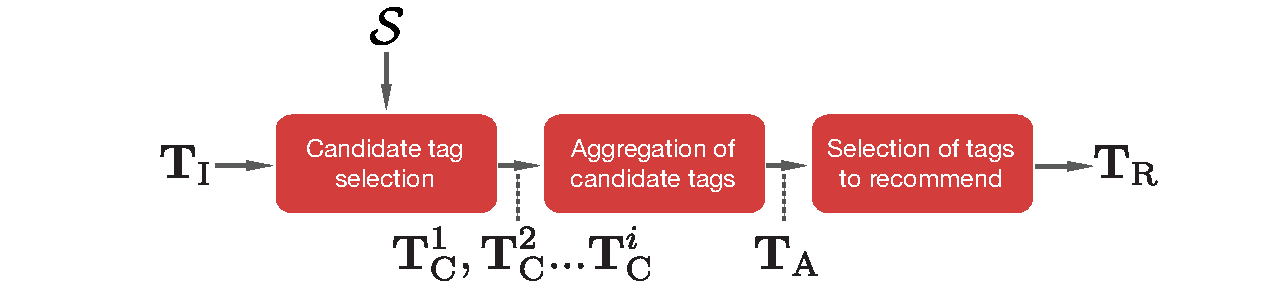
\includegraphics[width=\figSizeMax]{ch03_general/pics/00_diagram_alt.pdf}}
  \caption[Block diagram of the tag recommendation scheme]{Block diagram of the described tag recommendation scheme.}
  \label{general:fig:diagram}
\end{figure}

Given a set of input tags $\inputTags$ and a tag-tag similarity matrix $\similarityMatrix$ derived from a folksonomy $\folksonomy$, the general scheme for tag recommendation outputs a set of recommended tags $\recommendedTags$ (Fig.~\ref{general:fig:diagram}). 
%The folksonomy can be defined as a set of tag assignments $\folksonomy \subseteq \users \times \tags \times \resources$, where $\users$, $\tags$, and $\resources$ denote sets of users, tags, and resources, respectively~\cite{Mika2007a}\footnote{Mika~\citeyear{Mika2007a} uses the terminology Actor, Concept, and Instance ($A$, $C$ and $I$) to denote what we call User, Tag, and Resource ($\users$, $\tags$ and $\resources$). We adopted the latter terminology as it more closely relates with the data we are dealing with.}. 
The described scheme is composed of three independent steps: 1) Candidate tag selection, 2) Aggregation of candidate tags, and 3) Selection of tags to recommend. For Step 1, we propose three variants based on different similarity measures widely used in the literature~\citep[tag co-occurrence, cosine and Jaccard similarity;][]{halpin2006,jaske2007,Mika2007a,Sigurbjornsson2008,meo2009,Markines2009}. For Step 2, we propose two aggregation strategies (Similarity-based and Rank-based). For Step 3, we propose four selection strategies (Percentage, Statistical Test, Kernel Percentage and Linear Regression). What follows is a brief overview of these steps. In-depth descriptions are given in subsequent sections.

\begin{itemize}
  \item Step 1: Candidate tag selection. Given $\inputTags$ and a tag-tag similarity matrix $\similarityMatrix$ derived from $\folksonomy$, this step retrieves a set of $\nCandidateTagsPerInputTag$ candidate tags $\candidateTagsPerInputTag$ for each input tag $\inputTag$. %The retrieval of these candidates is based on tag-tag semantic similarity measures derived from $\folksonomy$.

  \item Step 2: Aggregation of candidate tags. This step takes the sets of candidates $\candidateTagsPerInputTag$, assigns a score value to each individual tag, and aggregates all candidates to form a single list of tags with assigned scores $\aggregatedCandidateTags$.

  \item Step 3: Selection of tags to recommend. This step automatically selects which tags to recommend given the candidate tags and score values of $\aggregatedCandidateTags$. The output of this step is the final set of recommended tags $\recommendedTags$.
\end{itemize}


\subsection{Candidate tag selection}
\label{sec:general:step1}

%Mika's model considers three finite sets of objects $\mathbf{A}$, $\mathbf{C}$ and $\mathbf{I}$ which correspond to ``actors'' (i.e.,~users), ``concepts'' (i.e.,~tags) and ``instances'' (i.e.,~resources). In this thesis, instead of the variables $\mathbf{A}$, $\mathbf{C}$ and $\mathbf{I}$ defined by ~\cite{Mika2007a}, we employ the notation $\users$, $\tags$ and $\resources$ respectively, which more closely relates to the ``users'', ``tags'' and ``resources'' terminology that we use.
%The sets of users, tags and resources are represented as nodes in the graph such that nodes $\vertices=\users\cup \tags\cup \resources$. The ternary relations between a user, a tag and a resource (i.e.,~tag applications) are then represented as the edges of the graph $\edges=\{\{\user,\tag,\resource\}| (\user,\tag,\resource)$ $\in \folksonomy\}$. Hence, the graph $\graph$ that represents a folksonomy $\folksonomy$ is finally defined as $\graph(\folksonomy)=\left\langle \vertices,\edges \right\rangle$. 
%The tripartite graph can be unfolded into a bipartite graph after discarding one of the three sets of nodes (i.e.,~$\users$, $\tags$ or $\resources$). In this way, it is possible to obtain the graph $\bipartiteGraphTagsUsers$ which relates tags and users, the graph $\bipartiteGraphUsersResources$ which relates users and resources, and the graph $\bipartiteGraphTagsResources$ which relates tags and resources. That last bipartite graph is the view of the folksonomy that we work with in this thesis, as it allows to derive relations between tags on the basis of their shared resources and vice versa.

We start the recommendation process by obtaining a number of related candidate tags to the set of input tags $\inputTags$. 
For each input tag $\inputTag$, we get a set of candidates $\candidateTagsPerInputTag$ by selecting the $\nCandidateTagsPerInputTag$ closest tags to $\inputTag$ according to a tag-tag similarity measure. For this purpose, we build a tag-tag similarity matrix $\similarityMatrix$ based on the tag assignment information contained in the folksonomy $\folksonomy$. Note that $\similarityMatrix$ is not dependent of the particular $\inputTag$ for which we are selecting candidates. Therefore, it only needs to be computed once for a given~$\folksonomy$\footnote{As is described later in Sec.~\ref{sec:general:datasets}, we filter out the least frequent tags of our folksonomy in order to reduce the computational complexity of $\similarityMatrix$.}. 

To represent the folksonomy $\folksonomy$, we use the model proposed by~\cite{Mika2007a}. Mika's model considers three finite sets of objects $\mathbf{A}$, $\mathbf{C}$ and $\mathbf{I}$, which correspond to ``actors'' (i.e.,~users), ``concepts'' (i.e.,~tags) and ``instances'' (i.e.,~resources), respectively. In this thesis, instead of the variables $\mathbf{A}$, $\mathbf{C}$ and $\mathbf{I}$ defined by ~\cite{Mika2007a}, we employ the notation $\users$, $\tags$ and $\resources$, which more closely relates to the ``users'', ``tags'' and ``resources'' terminology that we use.
The sets of users, tags and resources are represented as nodes in the graph such that the set of nodes $\vertices$ is defined as $\vertices=\users\cup \tags\cup \resources$. The ternary relations between a user, a tag and a resource (i.e.,~tag applications) are then represented as the edges of the graph $\edges=\{\{\user,\tag,\resource\}| (\user,\tag,\resource)$ $\in \folksonomy\}$. Hence, the graph $\graph$ that represents a folksonomy $\folksonomy$ is finally defined as $\graph(\folksonomy)=\left\langle \vertices,\edges \right\rangle$. 
%As we described in the previous chapter, Sec.~\ref{sec:soa:tag_recommendation_folkosnomy_analysis}, a folksonomy $\folksonomy$ can be naturally modelled as a tripartite hypergraph $\graph(\folksonomy)=\left\langle \vertices,\edges \right\rangle$, where vertices are given by three finite sets of objects, $\vertices=\users\cup \tags\cup \resources$, and each edge $\edges$ represents a tag-resource association performed by a user, $\edges=\{\{\user,\tag,\resource\}| (\user,\tag,\resource)$ $\in \folksonomy\}$ \citep{Mika2007a}. 

We unfold $\graph(\folksonomy)$ into the bipartite graph $\bipartiteGraphTagsResources$, which only reflects the associations between tags and resources. 
The bipartite graph $\bipartiteGraphTagsResources$ can be represented as a matrix $\associationMatrix = \left\{ \associationMatrixElement_{i,j} \right\}$, where $\associationMatrixElement_{i,j} = 1$ if tag $\tag_i$ has been used to label resource $\resource_j$, and $\associationMatrixElement_{i,j} = 0$ otherwise. 
We then define the matrix $\similarityMatrix$ so that
\begin{equation}
  \similarityMatrix = \associationMatrixMultiplication',
  \label{general:eq:Sim}
\end{equation}
which corresponds to a one-mode network connecting tags on the basis of shared resources~\citep{Mika2007a}. The symbol $'$ denotes matrix transposition. Elements $\similarityMatrixElement_{i,j}$ of $\similarityMatrix$ indicate the number of resources in which tags $\tag_i$ and $\tag_j$ appear together. Therefore, the diagonal of $\similarityMatrix$ represents the total number of different resources labelled with a tag $\tag_{i=j}$.

At this point, $\similarityMatrix$ can be interpreted as a tag-tag similarity matrix based on absolute co-occurrence. That is to say, the similarity between tags $\tag_i$ and $\tag_j$ is represented by the total number of times they appear together. This is the first similarity measure we use for our tag recommendation method. In order to obtain the rest of the aforementioned similarity measures, we apply different normalisation procedures to $\similarityMatrix$. Cosine similarity is defined as
\begin{equation}
  \similarityMatrixElement_{\tagb_i,\tagb_j} = \frac{\sum_{n} \associationMatrixElement_{i,n} \associationMatrixElement_{j,n} }{ \sqrt{\sum_{n} {\associationMatrixElement_{i,n}}^2} \sqrt{\sum_{n} {\associationMatrixElement_{j,n}}^2} } .
  \label{general:eq:CosineSim}
\end{equation}
Given that rows $\associationMatrixRow_i$ and $\associationMatrixRow_j$ are bit vectors (the only possible values are $0$ or $1$), $\sum_{n}{\associationMatrixElement_{i,n} \associationMatrixElement_{j,n}}$ is equivalent to the absolute co-occurrence between tags $\tag_i$ and $\tag_j$, while $\sum_{n}{\associationMatrixElement_{i,n}}^2$ and $\sum_{n}{\associationMatrixElement_{j,n}}^2$ is equivalent to the total number of occurrences of tags $\tag_i$ and $\tag_j$, respectively (the total number of resources labeled with $\tag_i$ and $\tag_j$). Therefore, cosine similarity can be obtained by dividing each element in $\similarityMatrix$ (Eq.~\ref{general:eq:Sim}) by $\sqrt{\similarityMatrixElement_{\tag_i,\tag_i} }\sqrt{\similarityMatrixElement_{\tag_j,\tag_j} }$. Similarly, the Jaccard index is defined as
\begin{equation}
  \similarityMatrixElement_{\tagb_i,\tagb_j} = \frac{\sum_{n} \associationMatrixElement_{i,n} \associationMatrixElement_{j,n} }{ \sum_{n} {\associationMatrixElement_{i,n}}^2 + \sum_{n} {\associationMatrixElement_{j,n}}^2 -  \sum_{n} \associationMatrixElement_{i,n} \associationMatrixElement_{j,n} } ,
  \label{general:eq:JacIndex}
\end{equation}
which is equivalent to dividing each element in $\similarityMatrix$ by $\similarityMatrixElement_{\tag_i,\tag_i} + \similarityMatrixElement_{\tag_j,\tag_j} - \similarityMatrixElement_{\tag_i,\tag_j}$. Independently of the similarity measure, $\similarityMatrix$ can be represented as a graph where nodes correspond to tags and edges represent the similarities between two tags (Fig.~\ref{general:fig:graph}).

Once we have a tag similarity matrix $\similarityMatrix$, we iterate over the input tags $\inputTags$ and get, for each element $\inputTag$, a set of candidates $\candidateTagsPerInputTag$. Specifically, we select the $\nCandidateTagsPerInputTag$ most similar tags to $\inputTag$ (i.e.,~the $\nCandidateTagsPerInputTag$ most similar graph neighbours of $\inputTag$) and keep these similarity values for further processing. Hence, for instance, if our method is fed with three input tags, it will get a maximum of $3\nCandidateTagsPerInputTag$ candidate tags (separated into three sets), provided that all three input tags have at least $\nCandidateTagsPerInputTag$ graph neighbours.

\begin{figure}
  \centerline{
  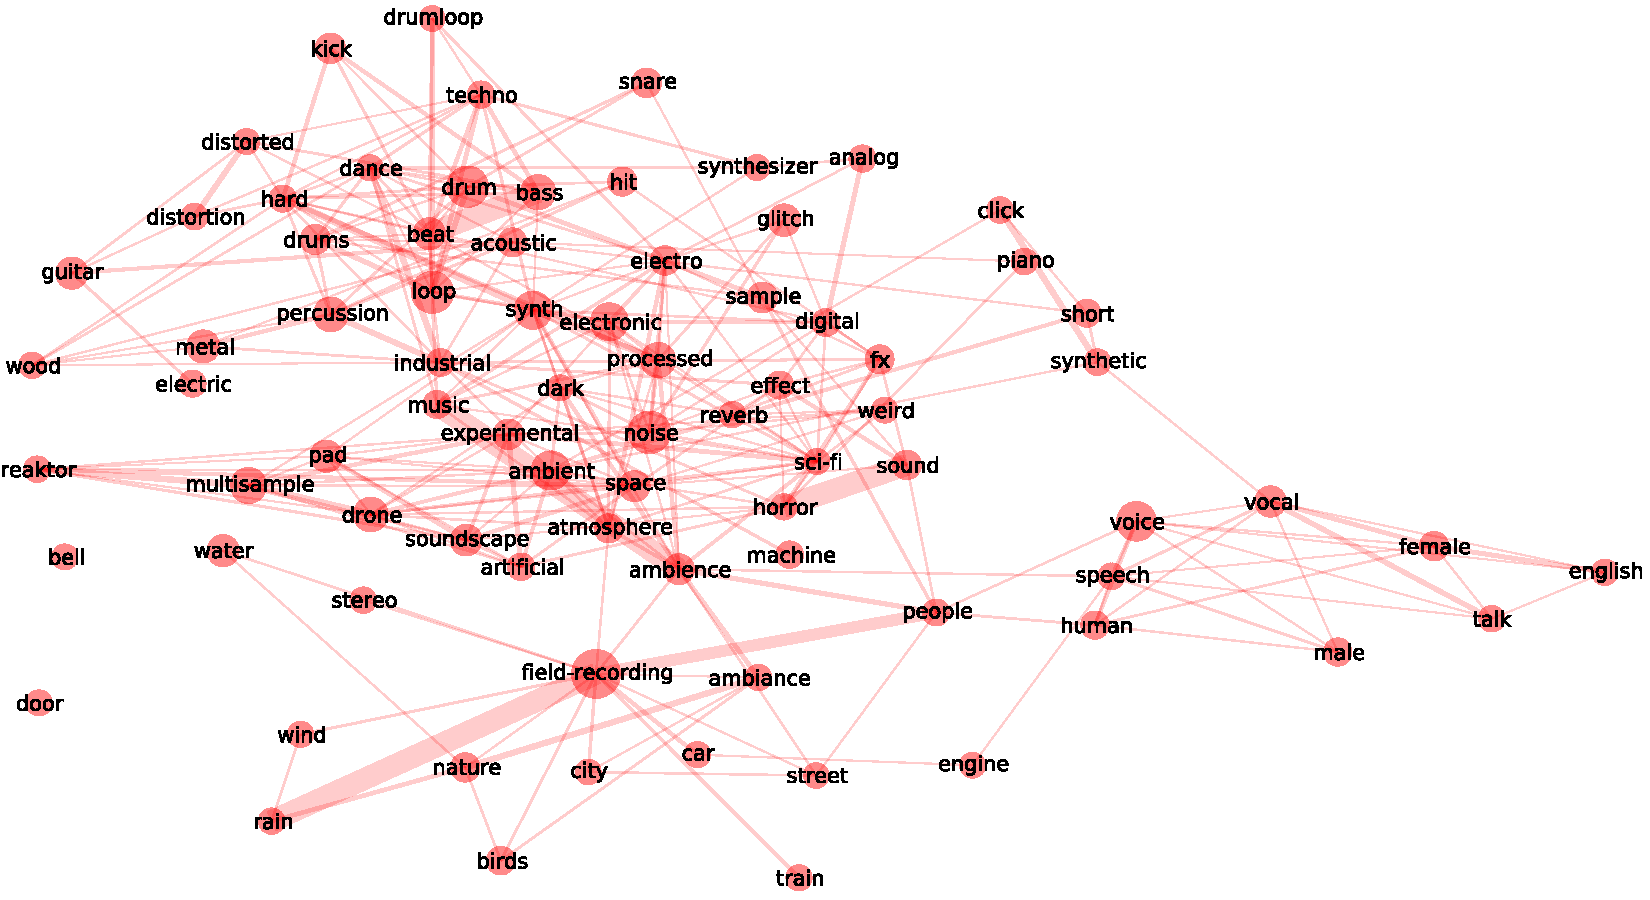
\includegraphics[width=\figSizeMax]{ch03_general/pics/01_graph_visualisation.pdf}}
  \caption[Graph visualisation of a tag-tag similarity matrix $\similarityMatrix$]{Graph visualisation of a tag-tag similarity matrix $\similarityMatrix$ built using cosine similarity and a subset of the Freesound folksonomy. Edge widths represent the cosine similarity between two tags. Tag size is a logarithmic function of the absolute tag frequency. For visualisation purposes, only edges above a certain degree of similarity and tags above a certain level of absolute frequency are shown.
  }
  \label{general:fig:graph}
\end{figure}


\subsection{Aggregation of candidate tags}
\label{sec:gen:step_2_aggregation}

The next step of our tag recommendation scheme takes all the sets of candidates $\candidateTagsPerInputTag$, assigns a score value $\scoreCandidateTag_j$ to every candidate $\candidateTag$ in $\candidateTagsPerInputTag$, and then aggregates all sets into a single list of tags with assigned scores $\aggregatedCandidateTags$. The output of this step, $\aggregatedCandidateTags$, is a list of tuples where each element contains a tag and an assigned score. To accomplish this step, we propose two different strategies:


\subsubsection{Similarity-based Strategy}

In the Similarity-based Strategy, the $j$-th candidate tag $\candidateTag$ of $\candidateTagsPerInputTag$ is assigned a score $\scoreCandidateTag_j$ that directly corresponds to the similarity value between the candidate tag and the corresponding input tag $\inputTag$, i.e.,~$\scoreCandidateTag_j = \similarityMatrixElement_{x,y}$, where $x=\candidateTag$ and $y=\inputTag$. After that, the list of tuples $\aggregatedCandidateTags$ is constructed as the union of all sets of candidates $\candidateTagsPerInputTag$ and their scores. 
If a particular tag has duplicates in $\aggregatedCandidateTags$ (which can happen if a given tag appears in several sets of candidates $\candidateTagsPerInputTag$), we only keep one occurrence and set its score to the sum of all the scores of the duplicates of that tag. This way we promote tags that are considered to be similar to more than one input tag. Moreover, as we do not want to recommend tags that are already part of $\inputTags$, we remove any occurrences of these tags in $\aggregatedCandidateTags$. 
We finally normalise the assigned scores by dividing them by the number of input tags $|\inputTags|$. 

\subsubsection{Rank-based Strategy}

The Rank-based Strategy only differs from the Similarity-based Strategy above in the way scores are assigned. Instead of directly using the similarity values from Step 1, we assign discrete ranks. For this purpose, we sort each set $\candidateTagsPerInputTag$ by similarity values in descending order, and assign scores as
$\scoreCandidateTag_j = \nCandidateTagsPerInputTag - (\positionOfCandidateTagInList -1)$, 
where $\positionOfCandidateTagInList$ is the position of the $j$-th tag in $\candidateTagsPerInputTag$ after sorting (thus $\positionOfCandidateTagInList$ ranges from 1 to $\nCandidateTagsPerInputTag$). Notice that the most similar tag to every input tag will be assigned a score of $\nCandidateTagsPerInputTag$. Even if a particular set $\candidateTagsPerInputTag$ contains less than $\nCandidateTagsPerInputTag$ tags (meaning that corresponding input tag $\inputTag$ has less than $\nCandidateTagsPerInputTag$ neighbours in the graph representation of $\similarityMatrix$), the score we assign to the most similar tag will be $\nCandidateTagsPerInputTag$. 
After score assignment, we proceed exactly as with Similarity-based aggregation: constructing $\aggregatedCandidateTags$ as the union of all sets $\candidateTagsPerInputTag$, merging duplicate tags in $\aggregatedCandidateTags$ by adding their scores, removing tags appearing in $\inputTags$, and normalising score values by $|\inputTags|$. An example comparing the result of the two aggregation strategies is shown in Table~\ref{tab:aggregation_examples}.

\begin{table}
\ra{1.1}
  \begin{center}
  \footnotesize
  \makebox[0pt]{
    \begin{tabular}{@{}l@{\hskip 1.0cm}lr@{\hskip 1.0cm}lr@{}}
      \toprule
      \multicolumn{1}{l}{}  &  \multicolumn{4}{c}{\textbf{ \textbf{Aggregated candidate tags (}$\mathbf{\aggregatedCandidateTags}$\textbf{)} }} \\ 
      \multicolumn{1}{l}{}  &  \multicolumn{2}{c}{\textbf{Similarity-based}} &  \multicolumn{2}{c}{\textbf{Rank-based}}  \\ 
      \textbf{\#} & \textbf{Tag} & $\mathbf{\scoreCandidateTag}$ & \textbf{Tag} & $\mathbf{\scoreCandidateTag}$ \\ 
      \midrule
      1 & \texttt{birds} & 0.307 & \texttt{birds} & 100.0  \\
      2 & \texttt{south-spain} & 0.244 & \texttt{ambiance} & 97.0  \\ 
      3 & \texttt{ambiance} & 0.229 & \texttt{south-spain} & 97.0  \\ 
      4 & \texttt{spring} & 0.180 & \texttt{summer} & 92.0  \\ 
      5 & \texttt{summer} & 0.169 & \texttt{spring} & 91.5  \\ 
      6 & \texttt{bird} & 0.162 & \texttt{bird} & 90.0  \\ 
      7 & \texttt{insects} & 0.157 & \texttt{thunder} & 82.5  \\
      8 & \texttt{donana} & 0.155 & \texttt{rain} & 82.0  \\ 
      9 & \texttt{ambience} & 0.151 & \texttt{ambience} & 80.0  \\ 
      10 & \texttt{forest} & 0.147 & \texttt{forest} & 79.5  \\
      11 & \texttt{thunder} & 0.145 & \texttt{weather} & 79.5  \\ 
      12 & \texttt{rain} & 0.139 & \texttt{field} & 79.0  \\ 
      13 & \texttt{marshes} & 0.139 & \texttt{water} & 77.5  \\ 
      14 & \texttt{weather} & 0.137 & \texttt{birdsong} & 75.5  \\
      15 & \texttt{water} & 0.129 & \texttt{purist} & 75.5  \\ 
      16 & \texttt{purist} & 0.129 & \texttt{donana} & 72.5  \\ 
      17 & \texttt{field} & 0.127 & \texttt{street-noise} & 71.5  \\
      18 & \texttt{birdsong} & 0.127 & \texttt{insects} & 71.5  \\ 
      19 & \texttt{street-noise} & 0.121 & \texttt{thunderstorm} & 70.0  \\
      20 & \texttt{atmos} & 0.118 & \texttt{storm} & 70.0  \\ 
      \multicolumn{1}{l}{}  &  \multicolumn{4}{c}{\rule{0pt}{3ex} \emph{+ 186 more}} \\
      \bottomrule
    \end{tabular}
    }
    \caption[Example of the output of the aggregation step]{Example of the output of the aggregation step using the Freesound folksonomy with $\inputTags=$ $\lbrace$\texttt{field-recording}, \texttt{nature}$\rbrace$ and $\nCandidateTagsPerInputTag=100$. Candidate tags are sorted by their score values. The score of $100$ for the tag \texttt{birds} in the Rank-based aggregation means that it is the most similar tag to both \texttt{field-recording} and \texttt{nature} ($100/2 + 100/2 = 100$). Notice that due to the use of different scoring methods, Similarity-based and Rank-based aggregation strategies produce different sorting of candidate tags and score distributions.}
  \label{tab:aggregation_examples}
  \end{center}
\end{table}


\subsection{Selection of tags to recommend}

Once we have computed $\aggregatedCandidateTags$, we select which of these tags should be recommended. For that, we consider four strategies that take into account the scores $\scoreCandidateTag$ of $\aggregatedCandidateTags$ to automatically determine a threshold $\scoreThreshold$.  The set of recommended tags $\recommendedTags$ is then formed by all the elements of $\aggregatedCandidateTags$ whose scores are equal to or above $\scoreThreshold$.


\subsubsection{Percentage Strategy}
\label{sec:general:percentage_strategy}

This is a straightforward strategy where $\scoreThreshold$ is determined as a percentage of the highest score in $\aggregatedCandidateTags$ by 
\begin{equation*}
  \scoreThreshold = (1-\percentageOfPercentageStrategy)\cdot \text{max}(\scoreCandidateTag) ,
\end{equation*}
where $\percentageOfPercentageStrategy$ is a percentage parameter that must be configured. Following the example shown in Table~\ref{tab:aggregation_examples}, and taking $\percentageOfPercentageStrategy=0.05$, only one tag would be recommended for the Similarity-based aggregation ($\scoreThreshold=(1-0.05)\cdot 0.307 = 0.292$; $\recommendedTags=$ $\lbrace$\texttt{birds}$\rbrace$) and three tags would be recommended for the Rank-based aggregation ($\scoreThreshold=(1-0.05)\cdot 100 = 95$; $\recommendedTags=$ $\lbrace$\texttt{birds}, \texttt{ambiance}, \texttt{south-spain}$\rbrace$).


\subsubsection{Kernel Percentage Strategy}

The Kernel Percentage Strategy has two steps. First, we estimate the probability density function $\probabilityDensityFunction$ of $\scoreCandidateTag$, the scores of $\aggregatedCandidateTags$. For that purpose, we use a kernel density estimator~\citep{silverman1986}, a fundamental data smoothing technique. The bandwidth of the kernel is automatically determined using Scott's Rule~\citep{scott2008}. Then, the threshold is defined as the $\scoreThreshold$ that satisfies
\begin{equation}
  \int_{\text{min}(\scoreCandidateTag)}^\scoreThreshold \probabilityDensityFunction(\scoreCandidateTag)\,\text{d}\scoreCandidateTag = (1 - \percentageOfKernelPercentageStrategy) \int_{\text{min}(\scoreCandidateTag)}^{\text{max}(\scoreCandidateTag)} \probabilityDensityFunction(\scoreCandidateTag)\,\text{d}\scoreCandidateTag ,
\end{equation}
where $\percentageOfKernelPercentageStrategy$ is a percentage parameter that must be configured. Therefore, $\percentageOfKernelPercentageStrategy$ determines the percentage of the area of the $\probabilityDensityFunction$ which we consider to include suitable tags for the recommendation (Fig.~\ref{general:fig:kde_percentage_example}). The bigger the parameter $\percentageOfKernelPercentageStrategy$, the smaller the threshold $\scoreThreshold$ becomes and thus the more tags are finally recommended.

The idea behind this strategy is that, understanding the scores of $\aggregatedCandidateTags$ as a sample extracted from a population of scores with an underlying distribution, the threshold $\scoreThreshold$ can be better determined by considering a percentage of the area of that underlying distribution rather than the percentage of the maximum observed score (as we propose in the Percentage Strategy above).


\subsubsection{Statistical Test Strategy}

Similarly to the previous strategy, here we also estimate the probability density function $\probabilityDensityFunction$ of $\scoreCandidateTag$ using a kernel density estimator. However, to determine the threshold $\scoreThreshold$, we follow an iterative process where, in each iteration, we select a slice of the $\probabilityDensityFunction$ and perform a statistical test for normality according to
\begin{equation}
  \label{general:eq:ad}
  \andersonDarlingTest(\probabilityDensityFunction_{\scoreThreshold : \text{max}(\scoreCandidateTag)}),
\end{equation}
where the function $\andersonDarlingTest$ is the Anderson-Darling test for normality~\citep{scho1987}, and $\probabilityDensityFunction_{\scoreThreshold : \text{max}(\scoreCandidateTag)}$ is the slice of $\probabilityDensityFunction$ that goes from $\scoreThreshold$ to $\text{max}(\scoreCandidateTag)$. 
In each iteration, $\scoreThreshold$ takes a different value such that 
\begin{equation}
  \scoreThreshold = \text{max}(\scoreCandidateTag) - i \cdot \frac{\text{max}(\scoreCandidateTag)-\text{min}(\scoreCandidateTag)}{100},
\end{equation}
where $i$ is the number of the current iteration ($i \in 1, 2, 3, ..., 100$). We stop the iterative process when the test fails for the first time (i.e.,~when the probability of having an independent normal distribution is not statistically significant). The final threshold takes the value of $\scoreThreshold$ at that iteration (Fig.~\ref{general:fig:kde_example}).

The idea behind this process is that, for a given set of candidate tags, there will be a subset of good tags for the recommendation exhibiting a normal and independent distribution, separated from the rest of candidates. The statistical test fails when it detects departures from normality and, according to our hypothesis, this will happen when non-meaningful candidate tags start affecting the $\probabilityDensityFunction$. Notice that this strategy, in practice, can be considered parameter-free as, by using the aforementioned Scott's rule, it only requires a statistical significance level from which to reject the null hypothesis of a normal distribution. We here follow common practice and take this significance level at 0.01~\citep{scho1987}. Using another common statistical significance level such as 0.05 would result in less restrictive statistical tests yielding bigger sets of recommended tags.

\begin{figure}[t]
  \centerline{
  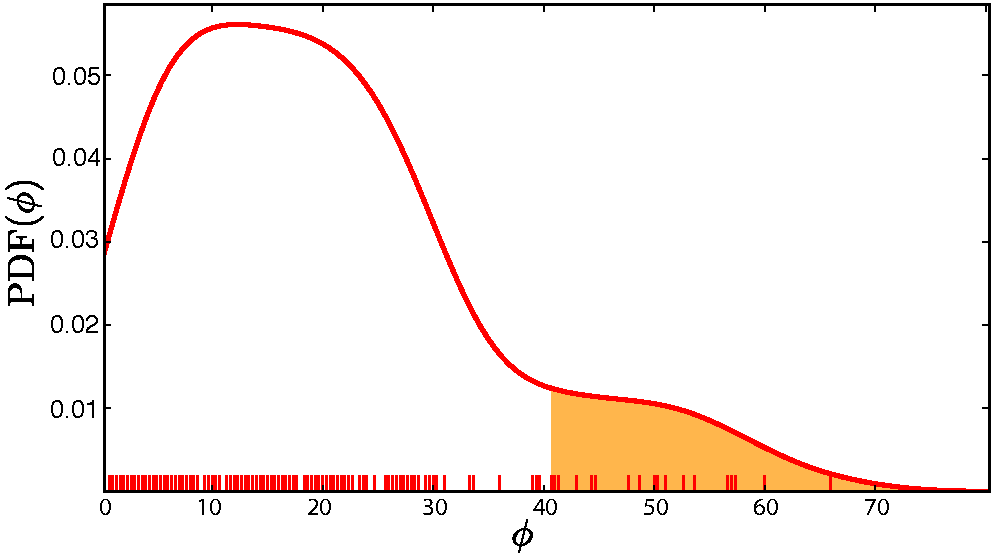
\includegraphics[width=\figSizeLarge]{ch03_general/pics/02_kernel_percentage_example.pdf}}
  \caption[Example of the Kernel Percentage Strategy for selecting which tags to recommend]{Example of the Kernel Percentage Strategy for selecting which tags to recommend (using $\percentageOfKernelPercentageStrategy = 0.05$). The curve represents the estimated $\probabilityDensityFunction$ of the scores of $\aggregatedCandidateTags$. Vertical markers on the horizontal axis show the actual positions of candidate tag scores. The shaded zone in the right of the figure corresponds to the 5\% of the total area of $\probabilityDensityFunction$. 
  Recommended tags are those under that zone.}
  \label{general:fig:kde_percentage_example}
\end{figure}

\begin{figure}
  \centerline{
  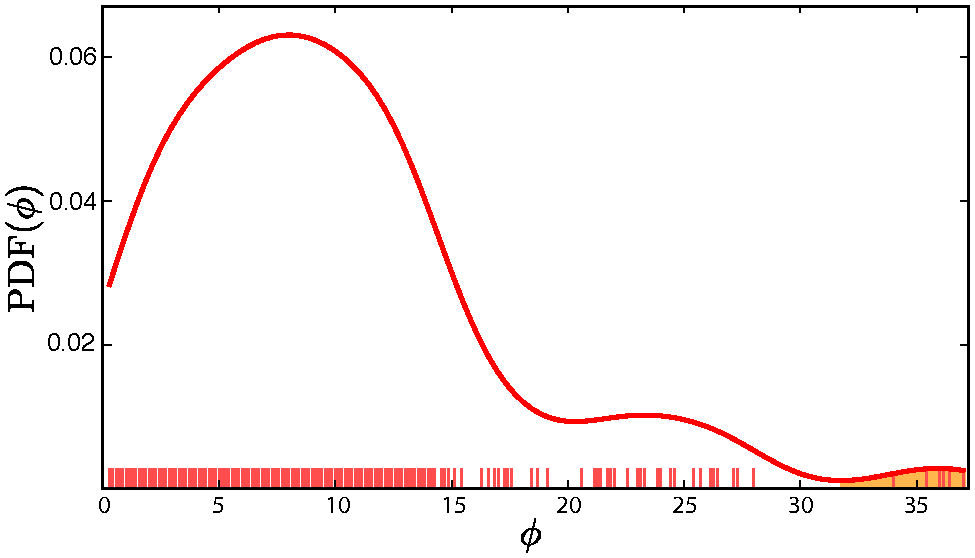
\includegraphics[width=\figSizeLarge]{ch03_general/pics/03_statistical_test_example.pdf}}
  \caption[Example of the Statistical Test Strategy for selecting which tags to recommend]{Example of the Statistical Test Strategy for selecting which tags to recommend. The curve represents the estimated $\probabilityDensityFunction$ of the scores of $\aggregatedCandidateTags$. Vertical markers on the horizontal axis show the actual positions of candidate tag scores. 
  Recommended tags are those under the shaded zone in the right. 
  In this example, the obtained threshold is $\scoreThreshold \approx 32$. Looking at the figure, it can be easily intuited that lower values of $\scoreThreshold$ would cause the statistical test of Eq.~\ref{general:eq:ad} to fail.}
  \label{general:fig:kde_example}
\end{figure}

\begin{figure}
  \centerline{
  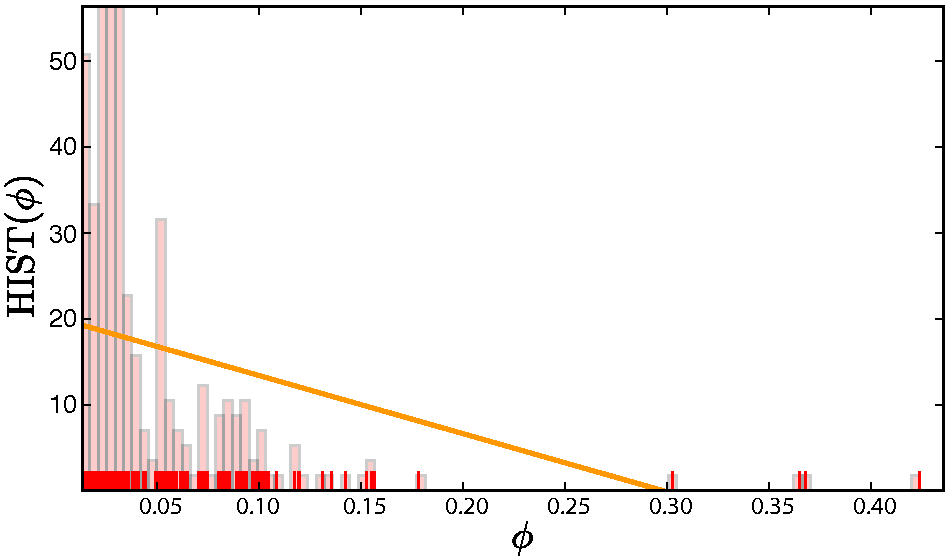
\includegraphics[width=\figSizeLarge]{ch03_general/pics/04_linear_regression_example.pdf}}
  \caption[Example of the Linear Regression Strategy for selecting which tags to recommend]{Example of the Linear Regression Strategy for selecting which tags to recommend. The straight line shows the linear regression of the histogram $\histogram$ of the scores of $\aggregatedCandidateTags$. Vertical markers on the horizontal axis show the actual positions of candidate tag scores. In this example, the obtained threshold is $\scoreThreshold \approx 0.29$, which is the point where the linear regression crosses the vertical axis. Recommended tags are those placed above 0.29.}
  \label{general:fig:polyfit_example}
\end{figure}


\subsubsection{Linear Regression Strategy}

The last strategy we propose consists in calculating the least-squares linear regression of the histogram $\histogram$ of $\scoreCandidateTag$. The threshold is set at the point where the linear regression crosses the vertical axis. 
The idea behind the Linear Regression Strategy is that, for a given $\histogram(\scoreCandidateTag)$, there will be a big concentration of candidate tags with low scores, and some outliers with bigger scores that will be separated from the rest (the most suitable tags for the recommendation). Thus, the linear regression will result in a straight line with a negative slope which will be useful to distinguish between both groups at the point where it crosses the vertical axis (Fig.~\ref{general:fig:polyfit_example}). The higher the concentration of low-scored candidates with respect to the outliers, the more pronounced the straight line will be, and the clearer the separation between both groups. 
Notice this strategy is also parameter-free.


\section{Evaluation}
\label{sec:general:evaluation_methodology}

From the combination of the different strategies above, we can define several tag recommendation methods which we evaluate through a tag prediction task (Sec.~\ref{sec:soa:evluation_of_tag_recommendation}). Essentially, what we do is to remove some tags from the resources of our datasets and then try to automatically predict them. In this section we describe the datasets and the methodology that we use for that evaluation.

\subsection{Datasets}
\label{sec:general:datasets}
We use two real-world datasets %(Table~\ref{tab:datasets}) 
collected from the tagging systems of Freesound and Flickr. In the case of Freesound, we consider all user annotations between April 2005 and September 2011, directly extracted from the Freesound database. From now on, we will refer to this dataset as \textsc{Freesound}. The Flickr data we use is a subset of photos taken in Barcelona, with user annotations performed approximately between January 2004 and December 2009. Flickr data was collected by~\cite{papadopoulos2010} and provided to us by the authors. To avoid confusion with the totality of the Flickr content, we will refer to the analysed Flickr subset as \textsc{Flickr1M}. Table~\ref{tab:datasets} shows some basic statistics about the folksonomies of both datasets.

\begin{table}
\begin{threeparttable}
\ra{1.2}
\footnotesize
  \begin{center}
    \makebox[0pt]{
    \begin{tabular}{@{}l@{\hskip 0.80cm}cc@{\hskip 0.5cm}cc@{}} %
      \toprule
      \multicolumn{1}{c}{} & \multicolumn{2}{c}{\textbf{Before filtering}} & \multicolumn{2}{c}{\textbf{After filtering}} \\ 
      \multicolumn{1}{c}{} & \textsc{Freesound} & \textsc{Flickr1M} & \textsc{Freesound} & \textsc{Flickr1M} \\ 
      \midrule
      Number of resources 		& 118,629 	& 107,617 	& 118,629 	& 107,617 \\ 
      Number of unique tags\tnote{a} 	& 33,790 	& 27,969 	& 6,232 	& 5,760 \\ 
      Number of contributor users\tnote{b} & 5,523 	& 5,463 	& 5,523 	& 5,463 \\ 
      Number of tag applications 	& 782,526	& 927,473 	& 730,417 	& 882,616 \\ 
      \bottomrule
    \end{tabular}
  }
    \begin{tablenotes}
    \item[a] Not necessarily semantically unique.
    \item[b] Users that have contributed by uploading, at least, one resource.
    \end{tablenotes}
  \caption[Basic statistics of the folksonomies of \textsc{Freesound} and \textsc{Flickr1M}]{Basic statistics of the folksonomies of \textsc{Freesound} and \textsc{Flickr1M} datasets. We see that the datasets feature comparable numbers. 
  The numbers under the ``After filtering'' column are computed by only considering tags that appear in at least 10 different resources (see below).}
  \label{tab:datasets}
  \end{center}
\end{threeparttable}
\end{table}

Freesound and Flickr have similar uploading processes in which users first provide the content (sounds and images, respectively) and then add as many tags as they feel appropriate to each resource\footnote{Since a software upgrade in 2011, Freesound requires a minimum of three tags to annotate a sound. However, the data we analyse is prior to the introduction of this requirement. In the case of Flickr, a single image can not be labeled with more than 75 tags, a large enough number not to be considered as a restriction for normal tagging behaviour.}. As opposed to other well-studied tagging systems such as Delicious or CiteULike, Freesound and Flickr feature a narrow folksonomy, meaning that resource annotations are shared among all users and, therefore, one single tag can only be assigned once to a particular resource (Sec.~\ref{sec:intro_tagging_systems_and_folksonomies}). Hence, we can not weigh the association between a particular tag and a resource by the number of times the same association has been performed by different users. 

\begin{figure}[t]
  \centerline{
  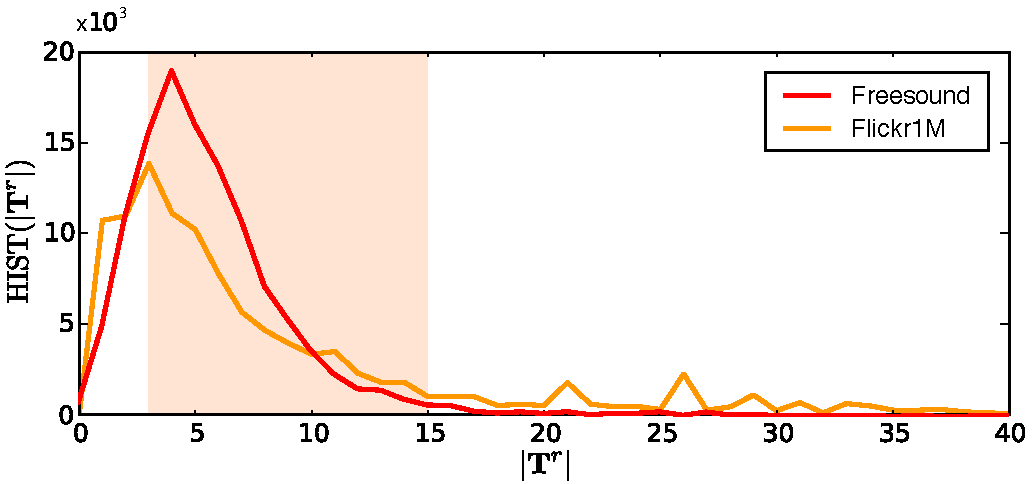
\includegraphics[width=\figSizeLarge]{ch03_general/pics/05_tag_distributions_B.pdf}}
  \caption[Histogram of the number of tags per resource in \textsc{Freesound} and \textsc{Flickr1M}]{Histogram of the number of tags per resource $|\tagsOfSoundR|$ in \textsc{Freesound} and \textsc{Flickr1M}. The average number of tags (standard deviation in parenthesis) per resource is 6.53 (6.47) and 7.50 (8.61) for \textsc{Freesound} and \textsc{Flickr1M}, respectively.}
  \label{general:fig:tag_distributions}
\end{figure}

The histogram of the number of tags per resource is qualitatively similar for the two datasets (Fig.~\ref{general:fig:tag_distributions}). We are particularly interested in recommending tags for resources that fall in the range of $|\tagsOfSoundR|=[3,15]$ tags, which are more than 80\% and 65\% of the total resources in \textsc{Freesound} and \textsc{Flickr1M}, respectively (Fig.~\ref{general:fig:tag_distributions}; shadowed zone). The reason for focusing on this range is that the tag recommendation scheme we propose takes as input the tags that have already been assigned to a resource. Thus, given the predictive nature of our evaluation (see below), we consider three tags as enough input information for our method to provide good recommendations. For resources with less than three tags, content-based strategies such as the ones outlined in Sec.~\ref{sec:soa:tag_recommendation_content_analysis} are probably more suited. On the other hand, we intuitively consider that resources with more than 15 tags are, in general, well enough described.

Among the set of all unique tags present in \textsc{Freesound} and \textsc{Flickr1M} folksonomies, we apply a threshold $\tagFrequencyThreshold=10$ to consider only the tags that have been used at least 10 times (i.e.,~tags that appear on at least 10 different resources). By this we assume that tags that have been used less than 10 times are irrelevant for our purposes. In addition, by discarding less frequent tags, we reduce the computational complexity of the calculation of $\similarityMatrix$ described in Step 1 (Sec.~\ref{sec:general:step1}). 
After applying this threshold, we are left with 6,232 unique tags in the \textsc{Freesound} folksonomy (representing approximately 20\% of the total) and with 5,760 unique tags in \textsc{Flickr1M} (also representing approximately 20\% of the total). This also means that we filter out all tag applications that do not associate any of these selected tags. Importantly, approximately 90\% of tag applications in both \textsc{Freesound} and \textsc{Flickr1M} involve one of these tags, thus we still take into account the vast majority of the original information (Table~\ref{tab:datasets}).


\subsection{Methodology}
\label{sec:general:evaluation_methodology_a}
Our evaluation methodology follows a standard information retrieval prediction task based on removing a number of tags from the resources of \textsc{Freesound} and \textsc{Flickr1M} and then trying to automatically predict them. The advantage of this approach is that it allows us to quickly evaluate the different recommendation algorithms without the need of human input. The main drawback is that tags that could be subjectively considered as good recommendations for a particular resource but are not present in the set of deleted tags, do not count as positive results. We mentioned this fact in Sec.~\ref{sec:soa:evluation_of_tag_recommendation} and further discuss it in Sec.~\ref{general:sec:discussion}.

For \textsc{Freesound} and \textsc{Flickr1M} datasets separately, we perform a 10-fold cross validation following the methodology described in~\cite{sal1997}. For each fold, we build $\similarityMatrix$ as described in Step 1, but only using the subset of the folksonomy corresponding to the training set of resources (i.e.,~only considering tag applications involving resources from the training set). For each resource in the evaluation set, we randomly delete a set of tags $\deletedTags$ from its originally assigned tags, yielding $\inputTags$, the input to our system. 
The number of tags we delete is chosen uniformly at random, with the only constraint that the length of $\inputTags$ must be maintained in the range of $|\inputTags|=[3,15]$ (see previous section). 
This constraint also implies that, in order to be able to remove at least one tag for each resource ($|\deletedTags| \geq 1$), we can only consider for evaluation resources with at least four tags. Furthermore, we add an upper limit to the number of tags and also filter out resources with more than 16 tags. We do that to avoid outliers with many tags which would result in very low recall values. 
Then, we run our tag recommendation methods using the tag similarity matrix $\similarityMatrix$ derived from the training set. 

Regarding evaluation measures, we compute $\precision$, $\recall$ and $\fmeasure$ as defined in Eq.~\ref{eq:prf_ch2} (Sec.~\ref{sec:soa:evluation_of_tag_recommendation}).
%for each individual resource according to
%\begin{equation}
%  \precision = \frac{|\recommendedTags \cap \deletedTags|}{|\recommendedTags|} \text{ }, \text{ }
%  \recall = \frac{|\recommendedTags \cap \deletedTags|}{|\deletedTags|} \text{ }, \text{ and }
%  \fmeasure = \frac{2\precision\recall}{\precision + \recall} \text{ ,}
%  \label{eq:prf_ch3}
%\end{equation}
%where $\recommendedTags$ is the set of recommended tags and $\deletedTags$ is the set of deleted tags. 
Then, global $\precision$, $\recall$ and $\fmeasure$ measures for each tag recommendation method are calculated by averaging $\precision$, $\recall$ and $\fmeasure$ across all resources evaluated with the particular recommendation method.
In addition to $\precision$, $\recall$ and $\fmeasure$, for each individual resource we also measure the number of recommended tags $|\recommendedTags|$. 
Evaluating $|\recommendedTags|$ is important because the longer the recommendation, the more comprehensive it potentially is, and the more difficult it is to maintain high precision values. We further discuss this aspect in Sec.~\ref{general:sec:discussion}. A general characterisation of the number of recommended tags per method is also obtained by averaging $|\recommendedTags|$ across all resources evaluated with a particular recommendation method.

\begin{table}
\begin{threeparttable}
  \ra{1.2}
  \begin{center}
  \footnotesize
  \makebox[0pt]{
    \begin{tabular}{@{}l@{\hskip 0.80cm}l@{\hskip 0.80cm}l@{}}
      \toprule
      \textbf{Name} & \textbf{Aggregation step} & \textbf{Selection step} \\
      \midrule
      \multicolumn{3}{c}{\emph{\rule{0pt}{4ex} Tag recommendation methods}}\\ 
      SimP@$\percentageOfPercentageStrategy$ & Similarity-based & Percentage ($\percentageOfPercentageStrategy=0.30$\tnote{a} , $\percentageOfPercentageStrategy=0.20$\tnote{b} )\\
      SimST & Similarity-based & Statistical Test \\ 
      SimKP@$\percentageOfKernelPercentageStrategy$ & Similarity-based & Kernel Percentage ($\percentageOfKernelPercentageStrategy=0.005$) \\ 
      SimLR & Similarity-based & Linear Regression\\ 
      RankP@$\percentageOfPercentageStrategy$ & Rank-based & Percentage ($\percentageOfPercentageStrategy=0.15$\tnote{a} , $\percentageOfPercentageStrategy=0.10$\tnote{b} )\\ 
      RankST & Rank-based & Statistical Test \\ 
      RankKP@$\percentageOfKernelPercentageStrategy$ & Rank-based & Kernel Percentage ($\percentageOfKernelPercentageStrategy=0.01$)\\ 
      RankLR & Rank-based & Linear Regression\\ 

      \multicolumn{3}{c}{\emph{\rule{0pt}{5ex} Baseline methods}}\\    
      BRankFIX@$\nRecommendedTagsInEvaluation$ & Rank-based & Fixed number ($\nRecommendedTagsInEvaluation \in [1,10]$) \\ 
      BSimFIX@$\nRecommendedTagsInEvaluation$ & Similarity-based & Fixed number ($\nRecommendedTagsInEvaluation \in [1,10]$) \\ %\cline{2-3}
      BRepeated@$\nRepeatedCandidateTags$ & \multicolumn{2}{c}{Repeated tags in all sets ${\candidateTagsPerInputTag}$($\nRepeatedCandidateTags \in [2,10]$)} \\ 
      BRandom & \multicolumn{2}{c}{Random replacement of $\recommendedTags$.} \\ 
      
      \multicolumn{3}{c}{\emph{\rule{0pt}{5ex} State of the art baseline methods}}\\ 
      GW@$\nRecommendedTagsInEvaluation$ & \cite{Garg2008} & Fixed number ($\nRecommendedTagsInEvaluation \in [1,10]$) \\ 
      SZ@$\nRecommendedTagsInEvaluation$ & \cite{Sigurbjornsson2008} & Fixed number ($\nRecommendedTagsInEvaluation \in [1,10]$) \\
      \bottomrule
    \end{tabular}
  }
  \begin{tablenotes}
    \item[a] Parameter settings for \textsc{Freesound} estimated in preliminary experiments. \item[b] Parameter settings for \textsc{Flickr1M} estimated in preliminary experiments.
  \end{tablenotes}
  \caption[List of evaluated tag recommendation methods]{Evaluated tag recommendation methods. All methods are evaluated using cosine similarity and $\nCandidateTagsPerInputTag=100$.}
  \label{tab:algorithms}
  \end{center}
\end{threeparttable}
\end{table}

Table~\ref{tab:algorithms} summarises all tag recommendation methods we evaluate. The first group of methods (Tag recommendation methods) are the eight possible combinations of aggregation and selection strategies that we propose. To avoid an intractable number of possible combinations, all methods are evaluated using only cosine similarity for Step 1, and setting $\nCandidateTagsPerInputTag=100$ (getting a maximum of 100 candidates for each input tag). 
We choose cosine similarity as default because of its widespread usage in the literature, and $\nCandidateTagsPerInputTag=100$ as an intuitively big enough number of candidates per input tag. 
We later study the influence of the chosen similarity measure and $\nCandidateTagsPerInputTag$, using only the highest performing methods of the main evaluation. For the methods that require the configuration of a percentage parameter (SimP@$\percentageOfPercentageStrategy$, SimKP@$\percentageOfKernelPercentageStrategy$, RankP@$\percentageOfPercentageStrategy$ and RankKP@$\percentageOfKernelPercentageStrategy$), we performed preliminary experiments with a subset of 10,000 resources from the main evaluation to determine the values of $\percentageOfPercentageStrategy$ and $\percentageOfKernelPercentageStrategy$ that reported higher average $\fmeasure$, and only consider these values in the main evaluation. 

Methods under the second group (Baseline methods, Table~\ref{tab:algorithms}) are simpler versions of the proposed methods that we use for comparative purposes. 
On the one hand, we compare with two methods that implement a very simple strategy for selecting which tags to recommend (Step 3) and always recommend the first $\nRecommendedTagsInEvaluation$ tags from $\aggregatedCandidateTags$, sorted by their scores (BRankFIX@$\nRecommendedTagsInEvaluation$ and BSimFIX@$\nRecommendedTagsInEvaluation$). We run these algorithms for values of $\nRecommendedTagsInEvaluation$ ranging from 1 to 10 and report only the best accuracy. 
Hence, the results reported for these methods constitute an upper bound of the accuracies that can be achieved when fixing the number of tags to recommend.
In preliminary experiments, we qualitatively observed a clear decrease of performance for values of $\nRecommendedTagsInEvaluation$ close to 10, therefore values $\nRecommendedTagsInEvaluation > 10$ are not considered (this also applies to other methods that have $\nRecommendedTagsInEvaluation$ as a parameter, see below).
On the other hand, we compare with an even simpler method (BRepeated@$\nRepeatedCandidateTags$) which, considering the union of all sets of candidates ${\candidateTagsPerInputTagOne}, {\candidateTagsPerInputTagTwo}, \text{... } \candidateTagsPerInputTag$ for a given resource, only recommends tags that are repeated more than $\nRepeatedCandidateTags$ times (independently of their scores). We run this algorithm for values of $\nRepeatedCandidateTags$ ranging from 2 to 10 and, as above, report only the best result found. 

We also compute a random baseline (BRandom) by replacing the set of $\recommendedTags$ with a random selection (of the same length) taken from $\aggregatedCandidateTags$. For each resource for which we recommend tags using any of the proposed methods above, we generate a random recommendation of the same length of $\recommendedTags$. Hence, for each proposed method, we also generate a randomised version of it. We take as the general random baseline the randomised version of all the proposed methods that reports higher $\fmeasure$.
Notice however, that these recommendations are not totally random: recommended tags are chosen from $\aggregatedCandidateTags$, not from the set of all possible tags in \textsc{Freesound} or \textsc{Flickr1M}. Moreover, by making a recommendation of the same length as the recommendation of the non-randomised version of the method, we preserve the distribution of the number of recommended tags for each method.

Finally, methods under the third group (State of the art methods, Table~\ref{tab:algorithms}) correspond to our implementations of the tag recommendation methods described by~\cite{Garg2008} and~\cite{Sigurbjornsson2008}, which we denote as GW and SZ, respectively. As these methods do not implement any selection step, we evaluate them for fixed values of $\nRecommendedTagsInEvaluation$ recommended tags ranging from 1 to 10 (and only report the best result found). \cite{Garg2008} describe several methods which contain different degrees of user personalisation. We implemented the ``global'' method which is not personalised and thus can be meaningfully compared to our methods. We implemented GW and SZ following the original references and set their parameters accordingly. 

\section{Results}
\label{sec:general:results}

\subsection{Recommendation accuracy}

From the average $\precision$, $\recall$ and $\fmeasure$ values for each one of the evaluated methods using the \textsc{Freesound} and \textsc{Flickr1M} datasets, we observe that Rank-based methods generally report higher $\fmeasure$ than Similarity-based methods (Tables~\ref{tab:results_freesound} and~\ref{tab:results_flickr}). Comparing the $\fmeasure$ values of each Rank-based method with its Similarity-based counterpart, we observe an average increase of 0.102 and 0.049 for \textsc{Freesound} and \textsc{Flickr1M}, respectively. We have assessed the statistical significance of this increase by performing pairwise Kruskal-Wallis tests~\citep{Corder2009} between the results of each Rank-based method and its Similarity-based counterpart, and all have shown to be statistically significant\footnote{In the rest of this chapter, in any comparison of $\fmeasure$ we indicate the results of the statistical significance tests as the maximum of the $\pvalue$-values of all pairwise comparisons.}, with a $\pvalue$-value several orders of magnitude below 0.01 (denoted as $\pvalue\ll0.01$). These results indicate that Step 2 (Aggregation of candidate tags) is better accomplished using the Rank-based Strategy.
% NOTE: statistical test was previously cited as wallis1952

Regarding the results of the different strategies for Step 3 (Selection of tags to recommend), we observe a very similar behaviour in \textsc{Freesound} and \textsc{Flickr\-1M} (Tables~\ref{tab:results_freesound} and~\ref{tab:results_flickr}, respectively). %That partially supports the generalisation of the proposed strategies to different kinds of data. 
In both datasets, methods using the Kernel Percentage Strategy (either with Rank-based or Similarity-based aggregation) perform significantly worse than the others, with an average $\fmeasure$ decrease of 0.036 for \textsc{Freesound} ($\pvalue\ll0.01$), and 0.048 for \textsc{Flickr1M} ($\pvalue\ll0.01$). Statistical Test, Linear Regression, and Percentage strategies report very similar $\fmeasure$, both in \textsc{Freesound} and \textsc{Flickr1M}, and specially in the case of Similarity-based aggregation. Nevertheless, the Percentage Strategy in combination with Rank-based aggregation provides the best obtained results in both datasets. When compared to the other selection strategies with Rank-based aggregation, it reports an average $\fmeasure$ increase of 0.025 for \textsc{Freesound} ($\pvalue\ll0.01$), and 0.039 for \textsc{Flickr1M} ($\pvalue\ll0.01$).
The similar results observed with \textsc{Freesound} and \textsc{Flickr1M} partially support the idea that the proposed methods are generalisable to different kinds of data.

\begin{table}[p] 
\ra{1.2}
\footnotesize
  \begin{center}
    \makebox[0pt]{
      \begin{tabular}{@{}lccc@{}}
      \toprule
  \multicolumn{4}{c}{\textsc{Freesound}} \\ 
  \textbf{Method} & \textbf{Precision} & \textbf{Recall} & \textbf{F-measure} \\ 
  \midrule
  RankP@0.15 & 0.444 & 0.532 & 0.437 \\ 
  RankST & 0.443 & 0.537 & 0.433 \\ 
  RankLR & 0.393 & 0.563 & 0.418 \\ 
  \textit{BRankFIX@2} & \textit{0.397} & \textit{0.468} & \textit{0.393} \\ 
  RankKP@0.01 & 0.352 & 0.524 & 0.383 \\ 
  \textit{GW@2} & \textit{0.375} & \textit{0.443} & \textit{0.371} \\ 
  SimLR & 0.347 & 0.397 & 0.324 \\
  SimP@0.30 & 0.344 & 0.414 & 0.323 \\ 
  SimST & 0.382 & 0.333 & 0.318 \\ 
  SimKP@0.005 & 0.356 & 0.294 & 0.294 \\ 
  \textit{BSimFIX@2} & \textit{0.303} & \textit{0.344} & \textit{0.293} \\ 
  \textit{SZ@2} & \textit{0.286} & \textit{0.334} & \textit{0.281} \\ 
  \textit{BRepeated@3} & \textit{0.176} & \textit{0.678} & \textit{0.235} \\ 
  \textit{BRandom (best)} & \textit{0.006} & \textit{0.033} & \textit{0.011} \\ 
  \bottomrule    
      \end{tabular}
    }  
    \caption[Average precision, recall and f-measure for tag recommendation methods using the \textsc{Freesound} dataset]{Average precision $\precision$, recall $\recall$ and f-measure $\fmeasure$ for tag recommendation methods using the \textsc{Freesound} dataset, sorted by f-measure. Baseline methods are marked in italics. For the sake of readability, we only show the results of baseline methods for the values of $\nRecommendedTagsInEvaluation$ and $\nRepeatedCandidateTags$ that reported higher f-measure.}
  \label{tab:results_freesound}
  \end{center}
\end{table}

\begin{table}[p] 
\ra{1.2}
\footnotesize
  \begin{center}
    \makebox[0pt]{
      \begin{tabular}{@{}lccc@{}}
      \toprule
  \multicolumn{4}{c}{\textsc{Flickr1M}} \\ 
  \textbf{Method} & \textbf{Precision} & \textbf{Recall} & \textbf{F-measure} \\ 
  \midrule
  RankP@0.10 & 0.503 & 0.513 & 0.452 \\ 
  \textit{GW@2} & \textit{0.480} & \textit{0.517} & \textit{0.442} \\ 
  \textit{BRankFIX@2} & \textit{0.475} & \textit{0.511} & \textit{0.441} \\ 
  RankST & 0.459 & 0.556 & 0.437 \\ 
  RankLR & 0.384 & 0.597 & 0.414 \\ 
  SimP@0.20 & 0.462 & 0.422 & 0.394 \\ 
  RankKP@0.01 & 0.389 & 0.483 & 0.388 \\ 
  SimST & 0.475 & 0.340 & 0.384 \\ 
  SimLR & 0.412 & 0.461 & 0.384 \\ 
  \textit{BSimFIX@2} & \textit{0.417} & \textit{0.440} & \textit{0.382} \\ 
  \textit{SZ@2} & \textit{0.384} & \textit{0.410} & \textit{0.353} \\ 
  SimKP@0.005 & 0.430 & 0.325 & 0.339 \\ 
  \textit{BRepeated@3} & \textit{0.163} & \textit{0.715} & \textit{0.219} \\ 
  \textit{BRandom  (best)} & \textit{0.007} & \textit{0.045} & \textit{0.020} \\    \bottomrule
      \end{tabular}
    }
    \caption[Average precision, recall and f-measure for tag recommendation methods using the \textsc{Flickr1M} dataset]{Average precision $\precision$, recall $\recall$ and f-measure $\fmeasure$ for tag recommendation methods using the \textsc{Flickr1M} dataset, sorted by f-measure. Baseline methods are marked in italics. For the sake of readability, we only show the results of baseline methods for the values of $\nRecommendedTagsInEvaluation$ and $\nRepeatedCandidateTags$ that reported higher f-measure.}
  \label{tab:results_flickr}
  \end{center} 
\end{table}

Having a look at the results of the baseline methods based on recommending a fixed number of tags (BRankFIX@$2$ and BSimFIX@$2$) we can see that, in terms of $\fmeasure$, they perform very similarly to the other proposed methods, and in some cases even outperform them (especially in the \textsc{Flickr1M} dataset). Importantly, we have to take into account that these baseline methods only vary from our proposed methods in the last step of the recommendation process, and that their reported results correspond to the upper bound of their performance (Sec.~\ref{sec:general:evaluation_methodology_a}). 
That good performance thus points out the effectiveness of the first two steps of the method in promoting the most relevant tags on the first positions of the list of candidates. If we compare these baseline methods with the state of the art implementations (GW@$2$ and SZ@$2$), we can see that our baselines get nearly equal or significantly higher $\fmeasure$ than those.
Regarding the other baselines, BRepeated@$\nRepeatedCandidateTags$ reports very low results both in \textsc{Freesound} and \textsc{Flickr1M} datasets, and BRandom baseline remains significantly below all the other methods.


\subsection{Number of recommended tags}

Another aspect to evaluate from the tag recommendation methods is the number of tags that they recommend $|\recommendedTags|$. 
Table~\ref{tab:number_of_recommended_tags} shows the average $|\recommendedTags|$ for the evaluated methods using the \textsc{Freesound} and \textsc{Flickr1M} datasets. We consider that methods which recommend higher number of tags and maintain overall high precision values are the most valuable for our purposes, as they provide both comprehensive and appropriate tag recommendations (i.e.,~relevant tags for the particular resource). 
In general we see that the best scoring methods, corresponding to the first positions of the table, recommend more tags than BRankFIX@2 and GW@2 (Table~\ref{tab:number_of_recommended_tags}), and at the same time report higher (or very similar) precision values and overall f-measure (see Tables~\ref{tab:results_freesound} and~\ref{tab:results_flickr}). If we look at the evaluation results obtained with BRankFIX@$\nRecommendedTagsInEvaluation$ methods when recommending more than two tags, we observe significant drops in precision ($\precision=0.323$ for $\nRecommendedTagsInEvaluation=3$ and $\precision=0.272$ for $\nRecommendedTagsInEvaluation=4$ in \textsc{Freesound}, and $\precision=0.391$ for $\nRecommendedTagsInEvaluation=3$ and $\precision=0.333$ for $\nRecommendedTagsInEvaluation=4$ in \textsc{Flickr1M}). Similar precision drops are observed in GW@$\nRecommendedTagsInEvaluation$ ($\precision=0.306$ for $\nRecommendedTagsInEvaluation=3$ and $\precision=0.257$ for $\nRecommendedTagsInEvaluation=4$ in \textsc{Freesound}, and $\precision=0.396$ for $\nRecommendedTagsInEvaluation=3$ and $\precision=0.340$ for $\nRecommendedTagsInEvaluation=4$ in \textsc{Flickr1M}).
This further highlights the superiority of our proposed methods over the baselines.

It is also interesting to see that the number of recommended tags is not only driven by the selection strategy of Step 3, but also depends on the type of aggregation used in Step 2. Both in \textsc{Freesound} and \textsc{Flickr1M}, we observe that when using Rank-based aggregation, highest $|\recommendedTags|$ is obtained using the strategy of Linear Regression for selecting which tags to recommend (followed by Statistical Test, Percentage and Kernel Percentage strategies). 
However, when using Similarity-based aggregation, the highest $|\recommendedTags|$ is obtained with the Percentage Strategy, followed by Linear Regression, Statistical Test and Kernel Percentage strategies  (Table~\ref{tab:number_of_recommended_tags}). This shows that the selection strategies behave differently if the scores of $\aggregatedCandidateTags$ are ranks or similarity values. In general, Rank-based methods recommend more tags than their Similarity-based counterparts, with an average $|\recommendedTags|$ increase of 0.38 for \textsc{Freesound} ($\pvalue\ll0.01$), and 0.86 for \textsc{Flickr1M} ($\pvalue\ll0.01$).
Given that Rank-based aggregation methods also report higher $\fmeasure$, this reinforces the aforementioned observation that Step 2 is better accomplished using the Rank-based Strategy.

\begin{table} \footnotesize
  \begin{center}
  \ra{1.2}
    \makebox[0pt]{
      \begin{tabular}{@{}lc@{\hskip 1cm}lc@{}}
      \toprule
  \multicolumn{2}{c}{\textsc{Freesound}} & \multicolumn{2}{c}{\textsc{Flickr1M}} \\ 
  \textbf{Method} & \textbf{$|\recommendedTags|$} & \textbf{Method} & \textbf{$|\recommendedTags|$} \\ 
  \midrule
  RankP@0.15 & 3.03 (2.60) & RankP@0.10 & 2.68 (1.96) \\ 
  RankST &  3.36 (3.30) & \emph{GW@2} &  \emph{2.00 (0.00)} \\ 
  RankLR &  3.55 (7.14) & \emph{BRankFIX@2} & \emph{2.00 (0.00)} \\ 
  \emph{BRankFIX@2} & \emph{2.00 (0.00)} & RankST & 3.96 (3.64) \\ 
  RankKP@0.01 & 2.89 (1.29) & RankLR & 4.64 (4.25) \\ 
  \emph{GW@2} &  \emph{2.00 (0.00)} & SimP@0.20 & 3.97 (1.64) \\    
  SimLR & 3.42 (2.36) & RankKP@0.01 & 2.60 (1.47) \\ 
  SimP@0.30 & 4.06 (3.10) & SimST & 1.98 (1.70) \\ 
  SimST & 2.35 (2.17) & SimLR & 3.15 (2.16) \\  
  SimKP@0.05 & 1.47 (0.70) & \emph{BSimFIX@2} & \emph{2.00 (0.00)} \\   
  \emph{BSimFIX@2} & \emph{2.00 (0.00)} & \emph{SZ@2} &  \emph{2.00 (0.00)} \\ 
  \emph{SZ@2} &  \emph{2.00 (0.00)} & SimKP@0.05 & 1.35 (0.73) \\ 
  \emph{BRepeated@3} & \emph{5.17 (8.17)} & \emph{BRepeated@3} & \emph{4.27 (3.11)} \\ 
  \emph{BRandom (best)} & \emph{5.17 (8.17)} & \emph{BRandom (best)} & \emph{4.27 (3.11)} \\ 
  \bottomrule
      \end{tabular}
    } 

    \caption[Average number of recommended tags per tag recommendation method]{Average number of recommended tags $|\recommendedTags|$ for tag recommendation methods using the \textsc{Freesound} and \textsc{Flickr1M} datasets (standard deviation into parentheses). Methods are displayed and sorted according to the $\fmeasure$ values of Tables~\ref{tab:results_freesound} and ~\ref{tab:results_flickr}. Baseline methods are marked in italics. } 
    %\vspace{0.8cm}
  
  \label{tab:number_of_recommended_tags} 
  \end{center}
\end{table}


\begin{figure}[t]
  \centering
  \subbottom[]{
    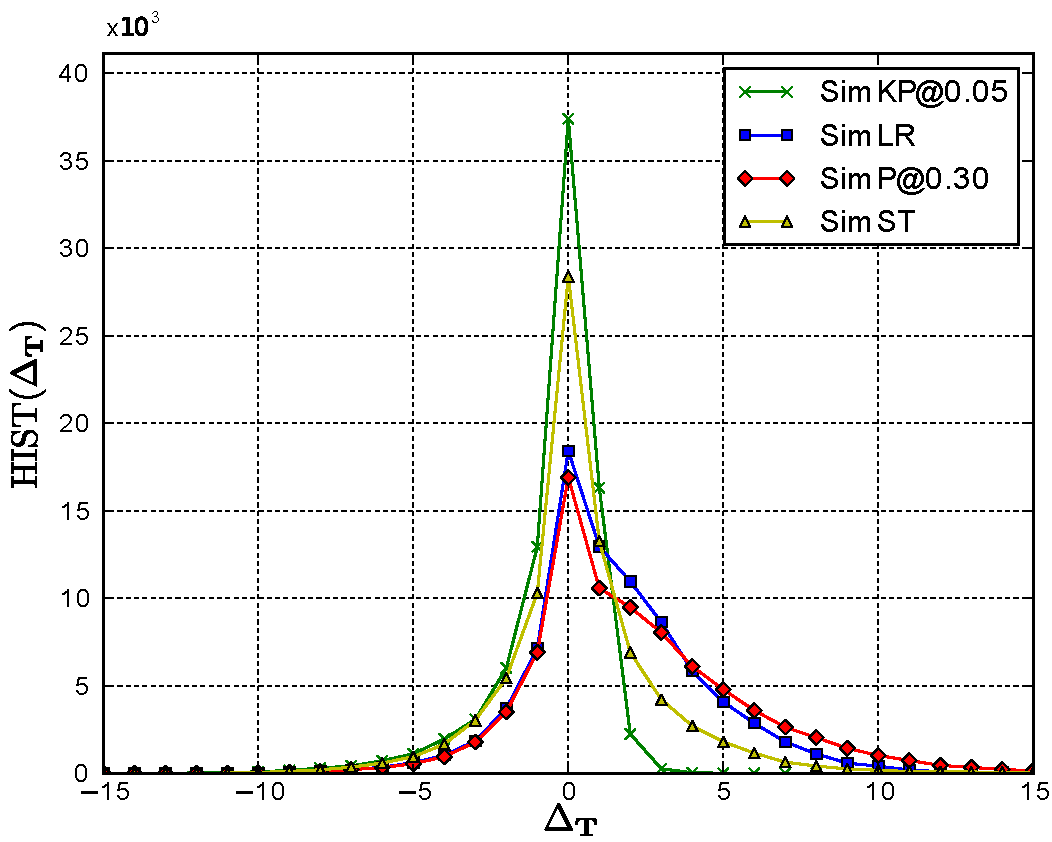
\includegraphics[width=\figSizeMid]{ch03_general/pics/06_similarity_based_hist2.pdf}}
  \subbottom[]{
    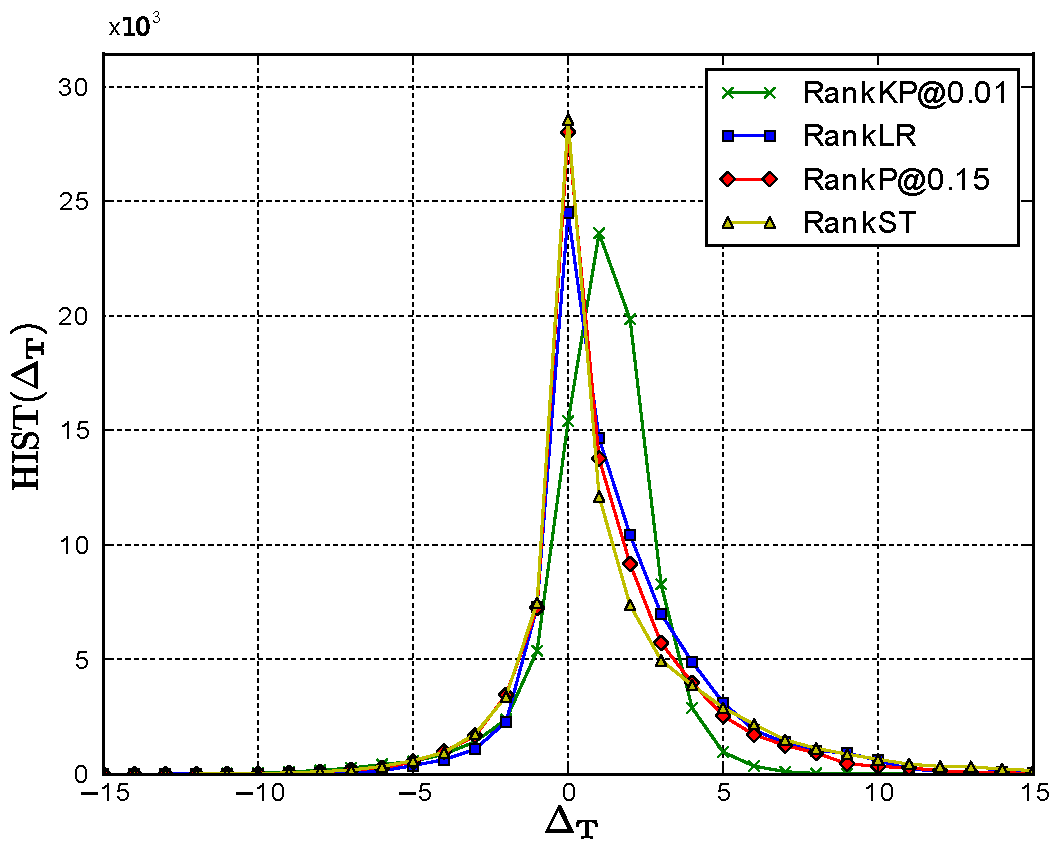
\includegraphics[width=\figSizeMid]{ch03_general/pics/07_rank_based_hist2.pdf}}
  \caption[Histogram of the difference between the number of recommended tags and the number of deleted tags]{Histogram of the difference between the number of recommended tags and the number of deleted tags $\differenceNRecTagsAndNDelTags$ for Similarity-based (a) and Rank-based (b) tag recommendation methods using \textsc{Freesound} dataset. Qualitatively similar results were obtained with \textsc{Flickr1M}.}
  \label{general:fig:hist}
\end{figure}

Furthermore, we also looked at the difference between the number of recommended tags and the number of tags that are deleted for each resource ($\differenceNRecTagsAndNDelTags = |\recommendedTags| - |\deletedTags|$). 
In Fig.~\ref{general:fig:hist} we show the histogram of $\differenceNRecTagsAndNDelTags$ for our proposed methods. We observe that most of our proposed methods report the maximum peak of the histogram at $\differenceNRecTagsAndNDelTags = 0$ (Fig.~\ref{general:fig:hist}). This suggests that these methods have a certain tendency to recommend as many tags as have been removed. 
Although it is not the goal of the tag recommendation methods to recommend the exact number of tags that have been removed (actually, this measure only makes sense under our tag prediction task-based evaluation), the results shown here are an interesting indicator that our proposed methods are able to indirectly estimate the number of deleted tags given only a set of input tags and the information embedded in the folksonomy. A plot of the average number of recommended tags as a function of the number of input tags and the number of deleted tags further supports this conclusion (Fig.~\ref{general:fig:added}). We can qualitatively observe how $|\recommendedTags|$ grows along with $|\deletedTags|$, specially for low $|\inputTags|$. 
It can also be observed that there is a tendency of $|\recommendedTags|$ increasing when $|\inputTags|$ decreases, meaning that the smaller the number of input tags, the more tags are recommended. 
Similar plots can be obtained with the other proposed recommendation methods, specially for RankLR and RankP (both in \textsc{Freesound} and \textsc{Flickr1M} datasets).


\subsection{Other relevant aspects}

In order to better understand the behaviour of the proposed tag recommendation methods, we have carried out further analyses on the influence of particular aspects of the methods. To avoid very intensive computation we have only focused on the three methods that report best average $\fmeasure$ both in \textsc{Freesound} and \textsc{Flickr1M}, that is to say, RankST, RankLR and RankP@$\percentageOfPercentageStrategy$ (with $\percentageOfPercentageStrategy$ being 0.15 for \textsc{Freesound} and 0.10 for \textsc{Flickr1M} as shown in Table \ref{tab:algorithms}). In the following sections we report experiments concerning these aspects.

\begin{figure}
  \centerline{
  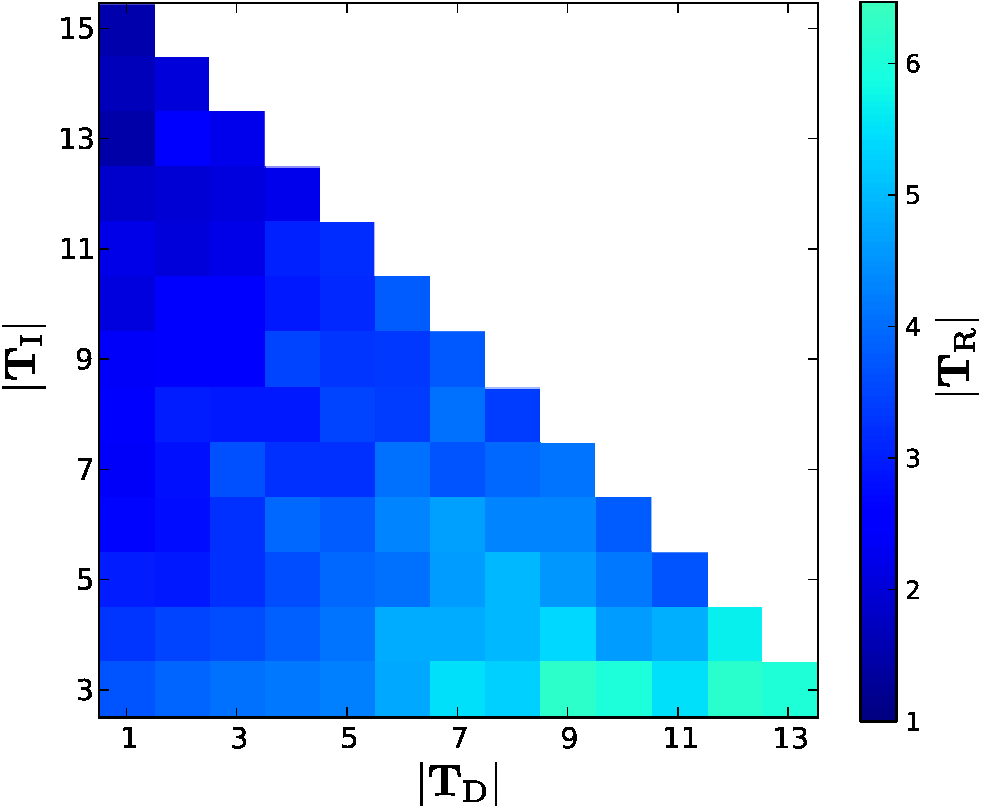
\includegraphics[width=\figSizeMid]{ch03_general/pics/08_recommended_tags_statistical_test.pdf}} 
  \caption[Average number of recommended tags as a function of the number of input tags and the number of deleted tags]{Average number of recommended tags $|\recommendedTags|$ as a function of  the number of input tags $|\inputTags|$ and the number of deleted tags $|\deletedTags|$, for method RankST and \textsc{Freesound} dataset.}
  \label{general:fig:added}
\end{figure}

\subsubsection{Limiting the minimum number of input tags}

To assess the influence of limiting the number of input tags, we now repeat the main experiments but include resources evaluated with less than three input tags. 
As it could be expected, we obtain lower $\fmeasure$ scores (Table \ref{tab:results_no_filt}).
On average, all methods have a decrease in $\fmeasure$  of 0.154 ($\pvalue\ll0.01$) and 0.141 ($\pvalue\ll0.01$) for \textsc{Freesound} and \textsc{Flickr1M} datasets, respectively. This confirms our initial observation that content-based methods might be more suited to recommend tags to scarcely labeled resources. In Fig.~\ref{general:fig:3d} we have plotted average $\fmeasure$ as a function of the number of input tags and the number of deleted tags for the RankP@0.15 method (using the \textsc{Freesound} dataset). This plot is useful to understand in which range of the number of input tags and number of deleted tags the recommendation performs better.  As it can be observed, the optimum conditions for high $\fmeasure$ are found with 5 or more input tags and 6 or less deleted tags, meaning that the recommendation needs a few input tags to effectively aggregate and select candidates and not many tags to predict.
Nevertheless, the fact that $\fmeasure$ is way above the random baseline of Tables~\ref{tab:results_freesound} and~\ref{tab:results_flickr} emphasizes that, even outside the optimum conditions, the proposed methods are still useful to some extent.


\begin{table} \footnotesize
\ra{1.2}
  \begin{center}
    \makebox[0pt]{
      \begin{tabular}{@{}lccc@{}}
      \toprule
	\textbf{Method} & \textbf{Precision} & \textbf{Recall} & \textbf{F-measure} \\  
	\midrule
  \multicolumn{4}{c}{\rule{0pt}{3ex}\textsc{Freesound}} \\ 
  
	RankP@0.15 & 0.323 & 0.375 & 0.297 \\  
	RankST & 0.337 & 0.326 & 0.285 \\  
	RankLR & 0.252 & 0.336 & 0.244 \\ 
	\multicolumn{4}{c}{\rule{0pt}{3ex}\textsc{Flickr1M}} \\ 
	RankST & 0.394 & 0.377 & 0.326 \\  
	RankP@0.10 & 0.329 & 0.434 & 0.309 \\  
	RankLR & 0.244 & 0.352 & 0.243 \\ 
  \bottomrule
      \end{tabular}
    }
    \caption[Average precision, recall and f-measure for the best scoring methods without filtering the number of input tags]{Average precision $\precision$, recall $\recall$ and f-measure $\fmeasure$ for the best scoring methods in \textsc{Freesound} and \textsc{Flickr1M} without filtering the number of input tags. Results are sorted in descending $\fmeasure$. }
    \label{tab:results_no_filt}
  \end{center}
\end{table}

\begin{figure}
  \centering
  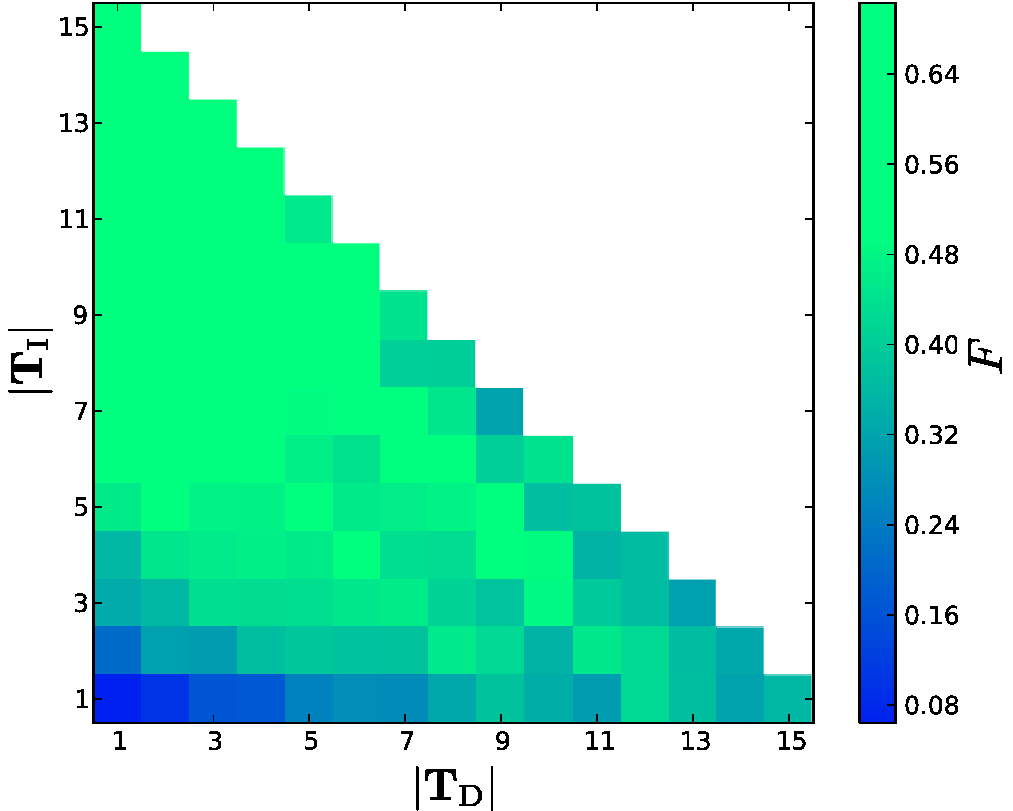
\includegraphics[width=\figSizeMid]{ch03_general/pics/09_fmeasure_percentage.pdf} 
  \caption[Average f-measure as a function of  the number of input tags and the number of deleted tags]{
  Average f-measure $\fmeasure$ as a function of  the number of input tags $|\inputTags|$ and the number of deleted tags $|\deletedTags|$ for method  RankP@0.15 and \textsc{Freesound} dataset. This plot includes the results of resources evaluated with fewer than three input tags.}
  \label{general:fig:3d}
\end{figure}


\subsubsection{Using alternative similarity measures}

As has been explained in the evaluation methodology, all previously reported experiments have been performed using cosine similarity as the similarity measure for Step 1. 
In this subsection we repeat the evaluation for the best scoring methods but now using Jaccard and tag co-occurrence as similarity measures (Table~\ref{tab:sims}). In both datasets and for all methods, cosine similarity is the metric that obtains higher $\fmeasure$, with an average increase of 0.009 ($\pvalue\ll0.01$, \textsc{Freesound}) and 0.053 ($\pvalue\ll0.01$, \textsc{Flickr1M}) respect to Jaccard, and 0.086 ($\pvalue\ll0.01$, \textsc{Freesound}) and 0.108 ($\pvalue\ll0.01$, \textsc{Flickr1M}) respect to tag co-occurrence. In the case of \textsc{Freesound}, we observe that the difference between cosine and Jaccard similarity is very small, and could be due to a marginal increase in the average number of recommended tags, thus lowering precision and getting a higher number of wrong recommendations. In \textsc{Flickr1M} the increase in the average number of recommended tags is more prominent, and so is the decrease in $\fmeasure$ for the methods using Jaccard distance.
We have observed that performing the same experiment with the Similarity-based counterparts of these methods (SimP@$\percentageOfPercentageStrategy$, SimST and SimLR) also leads to very similar results, with cosine similarity obtaining the highest $\fmeasure$ followed by Jaccard and tag co-occurrence. However, $\fmeasure$ differences among the different similarity measures tend to be slightly larger than these obtained with Rank-based methods.


\begin{table} \footnotesize
\ra{1.1}
  \begin{center}
  \makebox[0pt]{
    \begin{tabular}{@{}lcccc@{}}
    \toprule
      \textbf{Method} & \textbf{Precision} & \textbf{Recall} & \textbf{F-measure} & \textbf{$|\recommendedTags|$} \\ 
      \midrule
      \multicolumn{5}{c}{\rule{0pt}{4ex}\textsc{Freesound}} \\ 
      \multicolumn{5}{c}{\rule{0pt}{2ex} \emph{Cosine similarity}} \\ 
      RankP@0.15 & 0.444 & 0.532 & \textbf{0.437} & 3.03 \\ 
      RankST & 0.443 & 0.537 & 0.433 & 3.36 \\ 
      RankLR & 0.393 & 0.563 & 0.418 & \textbf{3.55} \\ 

      \multicolumn{5}{c}{\rule{0pt}{2ex} \emph{Jaccard similarity}} \\ 
      RankP@0.15 & 0.425 & 0.543 & \textbf{0.431} & 3.28 \\ 
      RankST & 0.421 & 0.552 & 0.423 & \textbf{3.91} \\ 
      RankLR & 0.370 & 0.570 & 0.405 & 3.84 \\ 

      \multicolumn{5}{c}{\rule{0pt}{2ex} \emph{Tag co-ocurrence}} \\ 
      RankP@0.15 & 0.339 & 0.483 & \textbf{0.352} & 3.37 \\ 
      RankST & 0.336 & 0.492 & 0.348 & 3.85 \\ 
      RankLR & 0.284 & 0.541 & 0.330 & \textbf{4.65} \\ 

      \multicolumn{5}{c}{\rule{0pt}{4ex}\textsc{Flickr1M}} \\ 
      \multicolumn{5}{c}{\rule{0pt}{2ex} \emph{Cosine similarity}} \\ 
      RankP@0.10 & 0.503 & 0.513 & \textbf{0.452} & 2.68 \\ 
      RankST & 0.459 & 0.556 & 0.437 & 3.96 \\ 
      RankLR & 0.384 & 0.597 & 0.414 & \textbf{4.64} \\ 

      \multicolumn{5}{c}{\rule{0pt}{2ex} \emph{Jaccard similarity}} \\ 
      RankP@0.10 & 0.417 & 0.491 & \textbf{0.397} & 3.46 \\ 
      RankST & 0.374 & 0.555 & 0.378 & \textbf{5.97} \\ 
      RankLR & 0.336 & 0.561 & 0.369 & 5.35 \\ 

      \multicolumn{5}{c}{\rule{0pt}{2ex} \emph{Tag co-ocurrence}} \\ 
      RankP@0.10 & 0.346 & 0.458 & \textbf{0.337} & 3.77 \\ 
      RankST & 0.320 & 0.505 & 0.329 & 5.43 \\ 
      RankLR & 0.269 & 0.542 & 0.311 & \textbf{6.12} \\ 
      \bottomrule
    \end{tabular}
  }
  \caption[Average precision, recall, f-measure and number of recommended tags using different similarity measures]{Average precision $\precision$, recall $\recall$, f-measure $\fmeasure$ and number of recommended tags $|\recommendedTags|$, using different similarity measures.}
  \label{tab:sims}
  \end{center}
\end{table}


\subsubsection{Number of candidate tags per input tag}

In order to understand the effect of the number of candidates per input tag $\nCandidateTagsPerInputTag$ (Step 1), we have performed a series of experiments with the best scoring methods. Similar to the main experiments described in Sec.~\ref{sec:general:evaluation_methodology_a}, we have performed 10-fold cross validations for each one of the best scoring methods, giving different values to $\nCandidateTagsPerInputTag$. To speed up computation time, we limited the number of resources of each experiment to 10,000. The rest of the parameters have remained constant (input tags in the range of $[3,15]$, using cosine similarity, and $\percentageOfPercentageStrategy=0.15$ or $0.10$ for \textsc{Freesound} and \textsc{Flickr1M}, respectively). The results show that most of the methods achieve a local maxima in the range of $\nCandidateTagsPerInputTag=[75,150]$, and then show a very slow decaying tendency (Fig.~\ref{general:fig:ns}). In \textsc{Freesound}, RankP@0.15 and RankST are shown to be more constant, without a 
noticeable decay (standard deviation of 0.005 for both RankST and RankP in the range of $\nCandidateTagsPerInputTag=[125,400]$). These results suggest that after selecting a sufficient amount of $\nCandidateTagsPerInputTag$ candidates for each input tag, the most relevant tags have already been selected, and increasing $\nCandidateTagsPerInputTag$ does not have a relevant impact on the output of the recommendation as score values for the ``extra'' candidates are generally low. 
According to Fig.~\ref{general:fig:ns}, for most of the methods, highest $\fmeasure$ is obtained with $\nCandidateTagsPerInputTag\approx 125$, which is slightly higher than the value we used for our main experiments ($\nCandidateTagsPerInputTag=100$). However, the average $\fmeasure$ increase is less than 1\%, and significance tests fail with $\pvalue \approx 0.10$ when comparing the methods configurations with $\nCandidateTagsPerInputTag=100$ and $\nCandidateTagsPerInputTag=125$.

\begin{figure}[t]
  \centerline{
  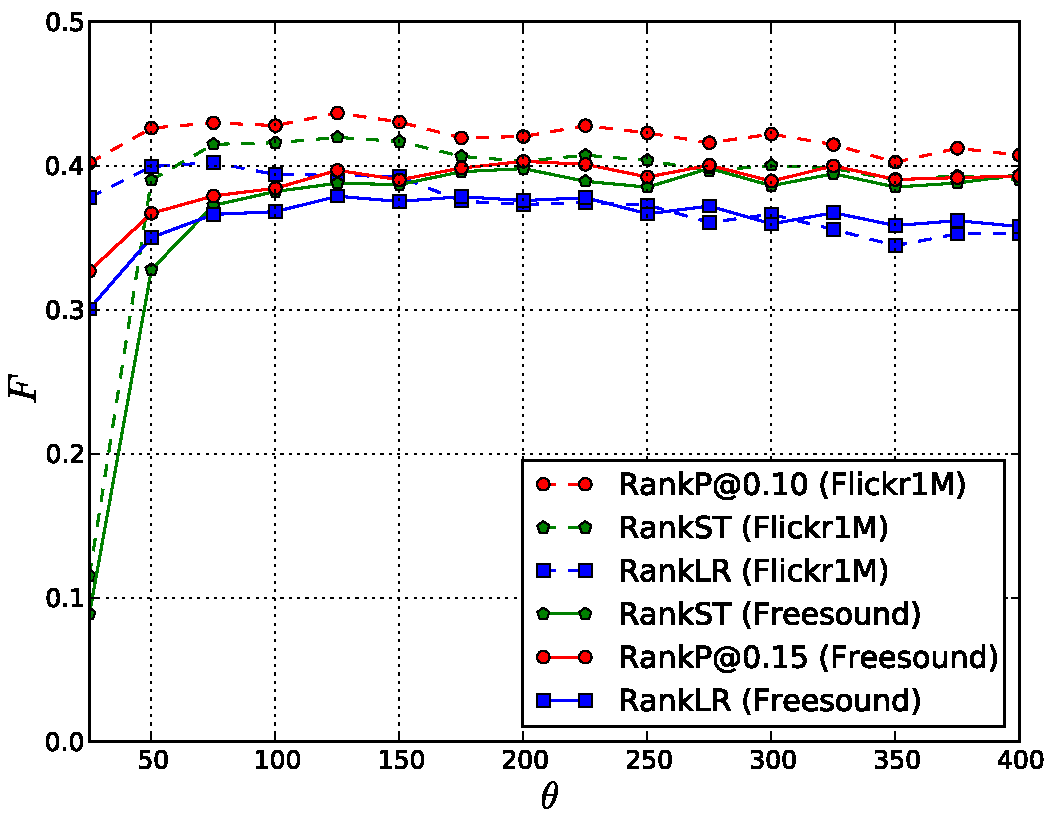
\includegraphics[width=\figSizeMid]{ch03_general/pics/10_fmeasure_per_N.pdf}}
  \caption[Average f-measure for different numbers of candidate tags per input tag]{Average f-measure $\fmeasure$ with different values of $\nCandidateTagsPerInputTag$ for the best scoring recommendation methods in \textsc{Freesound} and \textsc{Flickr1M} (each experiment performed with 10,000 resources).}
  \label{general:fig:ns}
\end{figure}

\subsubsection{Contribution of each step of the recommendation scheme}

To finish our analysis, we perform several experiments to evaluate the contribution of each step of the proposed tag recommendation scheme. For the best scoring methods, we have repeated the 10-fold cross validations of the main experiments three times, replacing in each run one step of the recommendation system by a randomised version of itself.
In the first run, we have replaced Step 1 by a random version that, for each input tag, selects $\nCandidateTagsPerInputTag$ random candidates from the whole vocabulary of the folksonomy (using $\nCandidateTagsPerInputTag=100$). 
In the second run we have maintained Step 1 as in the original setting, but have replaced Step 2 by an alternative version that, after performing a Rank-based aggregation, detaches the score values from each candidate in $\aggregatedCandidateTags$, and randomly re-assigns them among the candidates. 
Finally, in the third run of the experiments, we have maintained Steps 1 and 2 as in the original setting, but replaced the selection step by an alternative version that recommends the first $\nRecommendedTagsInEvaluation$ tags from $\aggregatedCandidateTags$ (sorted by the scores of candidates). In that case, $\nRecommendedTagsInEvaluation$ is determined by a random number generator with a normal distribution with the same mean ($\gaussianMean$) and standard deviation ($\gaussianStDev$) as that observed for the number of deleted tags in the main experiments ($\gaussianMean = 1.92$ and $\gaussianStDev = 1.58$ for \textsc{Freesound}, and $\gaussianMean = 2.32$ and $\gaussianStDev = 2.01$ for \textsc{Flickr1M}). By applying the distribution of the number of deleted tags to the number of recommended tags, we optimize $\fmeasure$ scores as precision and recall errors are minimised when $\differenceNRecTagsAndNDelTags \approx 0$.

Runs 1 and 2 report very low $\fmeasure$ in both datasets (Table~\ref{tab:random}). Run 3 obtains quite acceptable results, but with an average $\fmeasure$ decrease of 0.1270 ($\pvalue\ll0.01$, \textsc{Freesound}) and 0.1214 ($\pvalue\ll0.01$, \textsc{Flickr1M}) with respect to the normally working methods (without any randomisation). Hence, run 3 is still far from the optimum recommendation of normally working methods (Table~\ref{tab:random}). Given that Steps 1 and 2 are tightly coupled, failing in any of them has a very important impact on the final results. In the case of randomising Step 1, further steps can not effectively recommend tags as the original candidates are not relevant. When randomising Step 2, although candidate tags obtained in Step 1 are relevant, the aggregation can not assign meaningful scores to the candidates and thus the selection step fails in selecting which tags to recommend. Finally, when randomising Step 3, although a meaningful list of candidates can be sorted with meaningful score 
values, the number of tags that is recommended for each resource is selected in a completely unrelated way with respect to the score distribution of the candidates, thus not considering the possible relevance of each candidate given the other candidates. Overall, this demonstrates the usefulness of each of the three proposed steps in our tag recommendation scheme.

\begin{table} \footnotesize
\ra{1.2}
  \begin{center}
  \makebox[0pt]{
    \begin{tabular}{@{}l@{\hskip 1.0cm}cccc@{}}
    \toprule
      \multicolumn{1}{l}{\textbf{Method}} & \textbf{Run 1} & \textbf{Run 2} & \textbf{Run 3} & \textbf{No rand.} \\  %\textbf{No randomisation} \\ 
      \midrule
      \multicolumn{5}{c}{\rule{0pt}{3ex} \textsc{Freesound}} \\ 
      RankP@0.15 & $<$ 0.001 & 0.012 & 0.303 & 0.437 \\ 
      RankST & $<$ 0.001 & 0.006 & 0.302 & 0.433 \\ 
      RankLR & $<$ 0.001 & 0.007 & 0.302 & 0.418 \\ 
      \multicolumn{5}{c}{\rule{0pt}{3ex} \textsc{Flickr1M}} \\ 
      RankP@0.10 & $<$ 0.001 & 0.018 & 0.313 & 0.452 \\ 
      RankST & $<$ 0.001 & 0.010 & 0.313 & 0.437 \\ 
      RankLR & $<$ 0.001 & 0.011 & 0.312 & 0.414 \\ 
      \bottomrule
    \end{tabular}
  }
  \caption[Average f-measures after randomising steps of the best scoring tag recommendation methods]{Average f-measures $\fmeasure$ after randomising steps 1, 2 and 3 of the best scoring tag recommendation methods in \textsc{Freesound} and \textsc{Flickr1M}. The ``No rand.'' column shows the performance of the recommendation methods when no steps are randomised.}
  \label{tab:random}
  \end{center}
\end{table}

\section{Conclusion and discussion}
\label{general:sec:discussion}

In this chapter we have presented a general scheme for tag recommendation systems based on tag co-occurrence in folksonomies. This scheme is composed of three steps for which we have proposed different strategies. Step 1, Candidate tag selection, selects a number of candidate tags for every input tag based on a tag-tag similarity matrix derived from a folksonomy. Three variants of this step are given by the usage of alternative similarity measures. Step 2, Aggregation of candidate tags, assigns scores to the candidates from Step 1 and merges them all in a single list of candidate tags. For this step, we have proposed two strategies which differ in the way scores are assigned. Finally, Step 3, Selection of tags to recommend, automatically selects the candidates that will be part of the final recommendation by determining a threshold and filtering out those candidates whose score is below the threshold. For that last step we have described four strategies of different complexity levels. 

From the combination of these strategies, we have proposed eight tag recommendation methods and deeply evaluated them with two real-world datasets coming from two different online sharing platforms.
The main bottleneck in terms of scalability lies in the computation of the tag-tag similarity matrix that informs the candidate selection step. However, this matrix can be computed offline, and its size can be easily reduced by raising the threshold $\tagFrequencyThreshold$ during the construction of the association matrix. This means that the described recommendation methods can scale well to even bigger amounts of data, as the number of unique tags above the threshold $\tagFrequencyThreshold$ grows much more slowly than the number of resources.
Hence, the simplicity of the described methods makes them suitable for dealing with large-scale datasets such as the ones we have used here.
Moreover, the described tag recommendation methods are easily adaptable to any other tagging system featuring a narrow folksonomy, as recommendation is solely based on tag co-occurrence information regardless of the type of resources for which tags are being recommended. Evidence for supporting this statement can be directly extracted from the qualitatively similar results achieved with the two distinct datasets employed here.
We also compared our methods with simpler baselines and two state of the art methods described in the literature, and analysed the effects of several parameter configurations. Our exhaustive evaluation shows that the proposed methods can effectively recommend relevant tags given a set of input tags and a folksonomy embedding tag co-occurrence information.

An interesting aspect of the proposed tag recommendation scheme is the step focused on automatically selecting which tags to recommend given a list of candidates. 
Among the four strategies we have proposed, three of them  have been shown to effectively choose relevant tags for the recommendation and significantly improve the results (Percentage Strategy, Statistical Test Strategy and Linear Regression Strategy). These three strategies reported qualitatively similar results, though the good performance of the Statistical Test and the Linear Regression strategies is of special relevance as both can be considered parameter-free. We have also shown that scoring candidate tags using ranks instead of raw tag similarities significantly increases the accuracy of the recommendations.

Much of the evaluation we have conducted is based on analysing the f-measure obtained after a tag prediction task. Although such systematic approach allows us to compare the different tag recommendation methods using a large number of resources, the results in terms of f-measure are probably much worse than what a user-based evaluation could have reported~\citep{Garg2008}. To exemplify this observation, Table~\ref{tab:examples} shows a few examples of tag recommendations performed using the RankST method in the \textsc{Freesound} dataset. We have bolded the tags that are considered good recommendations under our evaluation framework. Notice however that many of the recommended tags which are not bolded could also be judged as meaningful recommendations if we actually listen to the sounds. Moreover, our systematic evaluation does not take into account other aspects of the recommended tags such as their semantic context or their informational value in the folksonomy. 
%We think that future research should consider these kind of aspects, and tag recommendation systems should include domain-specific knowledge to provide more meaningful recommendations. 

%Constructing better tag recommendation systems yielding more useful tag descriptions of online resources would allow improved organisation, browsing and reuse of online content.
%But not only that. In the literature on social and semantic web there have been many discussions regarding the relevance and value of folksonomies compared to ontologies and vice versa \cite{shirky2005ontology,Mika2007a,gruber2007ontology,al2007exploring}. In some cases, both concepts appear as opposed approaches for bottom-up (folksonomies) or top-down (ontologies) knowledge sharing. However, many authors coincide in that both approaches can coexist and reciprocally benefit from each other. In this direction, many studies have been performed around the idea of extracting structured knowledge from folksonomies \cite{limpens2009linking}. We too believe that folksonomies are a powerful tool from which relevant structured knowledge can be gathered, and that they have to play a very important role in the semantic web. By using approaches such as the one we have presented here, more coherent and less noisy folksonomies can emerge and we can help leveraging their value as reliable sources for knowledge-mining and ontology-induction.

Overall, the work we have carried out shows that the proposed scheme for folksonomy-based tag recommendation can successfully be used for recommending tags to online resources.
In the following chapter, we propose an improvement for the best-scoring recommendation method described here, and carry out an evaluation based on user assessment of the recommended tags.

\begin{table} \footnotesize
  \ra{1.2}
  \begin{center}
  \makebox[0pt]{
    \begin{tabular}{@{}lP{3.3cm}p{2.4cm}p{3.6cm}l@{}}
    \toprule
      \textbf{Sound id} & \textbf{Input tags} & \textbf{Deleted tags} & \textbf{Recommended tags} & $\fmeasure$ \\ 
      \midrule
      8780 & analog, glitch, warped & lofi & noise, electronic & 0.0 \\ 
      124021 & \raggedright newspaper, reading, paper, page, news & read & magazine & 0.0 \\ 
      38006 & hit, glass, oneshot & percussion & \raggedright singlehit, singlebeat, single, tap, hits, house, \textbf{percussion}, place, thuds, drum, plock &  0.17 \\ 
      54374 & \raggedright spring, nightingale, nature, bird & \raggedright field-recording, birdsong, binaural & \raggedright birds, \textbf{field-recording}, forest, \textbf{birdsong} & 0.5 \\ 
      78282 & \raggedright metal, medium-loud, interaction & impact & \textbf{impact}, wood & 0.67 \\    
      \bottomrule
    \end{tabular}
  }
  \caption[Example tag recommendations performed in \textsc{Freesound}]{Example of tag recommendations in \textsc{Freesound} using the RankST method. Corresponding sounds can be listened at the following url: \url{http://www.freesound.org/search?q=}[Sound id].}
  \label{tab:examples}
  \vspace{13cm}
  \end{center}
\end{table}




\cleartorecto%!TEX root = ../thesis_a4.tex

\chapter[An enhancement: class-based tag recommendation][An enhancement: class-based tag rec.]{An enhancement: class-based tag recommendation}
\label{sec:class}

\section{Introduction}
\label{sec:class:introduction}

%Free-form semantically-meaningful textual labels, called tags, are extensively used in online sharing platforms for describing and annotating contents. Systems that provide the functionality for making these annotations are normally referred to as collaborative tagging systems. Several problems arise when users annotate shared and/or online resources~\citep{halpin2006}. The most typical ones are tag scarcity, the use of different tags to refer to a single concept (synonymy), the ambiguity in the meaning of certain tags (polysemy), the commonness of typographical errors, the use of user-specific naming conventions, or the use of different languages. To minimise some of these problems, tag recommendation systems can be employed to suggest potentially relevant tags during the annotation process~\citep{jaske2007}. As users are exposed to the suggestions of the system, the annotation process partially shifts from the creation of textual labels to the recognition of tags in a list~\citep{Sood2007}, and thus all users receive a certain common influence from the system. Hence, tag recommendation serves the purpose of consolidating the vocabulary of collaborative tagging systems~\citep{Jaschke2009}.

%In general, tag recommendations are either based on content analysis of online resources or in the other tags that users introduce during the annotation process. In the case of content-based recommendations, a typical approach consists in, given a resource to be described, defining a neighbourhood of other resources (based on some similarity measure) and then recommending tags that are used to annotate resources in this neighbourhood~\citep{ivanov2010, moha2012}. Another approach is the use of machine learning techniques to learn mappings between tags and content features~\citep{Li2006, turnbull2008, Toderici2010}. On the other side, there are tag recommendation strategies which are based on the tags that users introduce during the annotation process itself, prior to the moment of the recommendation. 
%Disadvantages of these strategies compared to content-based recommendation methods are that they require the existence of at least one tag to provide recommendations, whereas content-based recommendation systems can provide recommendations to resources with no associated tags or other metadata.
%Nevertheless, tag recommendation methods based on the tags that users introduce during the annotation process have the advantage of not requiring any specific processing of the content of the resources being annotated, thus being typically less expensive in terms of computation resources and being more easily generalisable to other multimedia domains.
%These methods usually consider the \emph{folksonomy} (i.e.,~the set of associations between tags, users and content resources) of a collaborative tagging system to estimate tag similarity from their resource co-occurrence. In this way, candidate tags can be selected according to their similarity to the introduced tags, and a sorting algorithm can rank them in terms of estimated relevance~\citep{jaske2007, Sigurbjornsson2008, Garg2008, DeMeo2009}. In previous work, we described and evaluated a general scheme for folksonomy-based tag recommendation in collaborative tagging systems~\citep{Font2013}. Out of that scheme, eight particular methods were proposed which form the basis of the method presented in this work.

%Besides content-based and folksonomy-based tag recommendation systems, other approaches have been described in the literature. Anderson et~al.~\citep{Anderson2008} describe a tag recommendation system for Flickr\footnote{\texttt{www.flickr.com}}, a well known photo sharing site, which combines both content-based recommendations (by training a predictive model that learns the mapping between tags and extracted content image features) with folksonomy-based recommendations (following an strategy very similar to~\citep{Sigurbjornsson2008}). Naaman and Nair\citep{Naaman2008} describe another tag recommendation system for Flickr, which takes advantage of the geolocation metadata attached to images and recommends tags that other users employed in close areas. Chen et~al.~\citep{Chen2010} describe a tag recommendation system for video resources which crawls the web for information about these videos and identifies keywords to recommend as tags.

%Although it is quite common to personalise tag recommendation systems to the tagging behaviour of particular users by promoting, for example, tags that users introduced in past annotations~\citep{jaske2007, Garg2008, Lipczak2008, Rendle2009, Marinho2009, Cao2009}, most of the current systems do not introduce direct user feedback in the evaluation loop. Thus recommendations are generally evaluated using traditional information retrieval approaches based on the comparison of tag rankings produced by different methods, or using precision and recall metrics computed after a tag prediction task~\citep{Garg2008, Lipczak2008, Rendle2009, Cao2009, Marinho2009, Font2013}. 
%To the best of our knowledge, only three studies perform some kind of user-based evaluation. Sigurbj\"{o}rnsson and Zwol~\cite{Sigurbjornsson2008} automatically generate tag recommendations for several images from a Flickr dataset and then ask users to rate, in a four-point scale, whether the recommendations are appropriate to a given image. 
%Similarly, De Meo et~al.~\cite{DeMeo2009} extend the annotations of Delicious' bookmarks\footnote{\texttt{www.delicious.com}} and then ask users to evaluate the relevance of every tag/resource association. 
%J\"{a}schke et~al.~\cite{Jaschke2009} perform a small evaluation based on a real-world scenario where users have to tag bookmarks in BibSonomy\footnote{\texttt{www.bibsonomy.org}}. Specifically, precision and recall metrics are computed by comparing tag recommendations performed to every bookmark and the final taglines that users introduced. Due to its subjectiveness and many different ways to be accomplished, tag recommendation is not an easy task to evaluate, and some advantages and disadvantages can be found in both user-based and information retrieval evaluation approaches~\citep{Garg2008}.
%However, there is a clear lack of user-based evaluation in previous work, and we believe that every recommendation system should be validated at some point using both evaluation strategies. Proper user feedback should be helpful not only to compare tag recommendation methods but also to better understand the nature of the task and learn how can systems be improved.

In this chapter we build on the tag recommendation methods described in the previous chapter and extend them. Furthermore, we perform an evaluation of the extended recommendation system through an online experiment with real users. Hence, the contribution of the present chapter is twofold. 
Firstly, we propose an extended version of the best performing tag recommendation method described in Chapter~\ref{sec:general} (RankP@$\percentageOfPercentageStrategy$). The main idea behind this extended method is to exploit the automatic classification of the resources to be annotated into a number of predefined classes to further adapt the tag suggestions to the context of these classes. This classification is based on the tags that users start introducing during the annotation process. In this way, instead of personalising recommendations for particular users, we ``personalise'' them to particular classes of resources, and the extended tag recommendation system incorporates some domain-specific knowledge in the form of resource categories.
We evaluate the automatic classification process separately from the rest of the tag recommendation system.

Secondly, we perform a comprehensive user-based evaluation through an online experiment. In it, participants are presented with some resources which have to be annotated with the help of the tag recommendation system. 
These kinds of user-based evaluations are very costly, and we have seen that they are not very common in the tag recommendation literature (Sec.~\ref{sec:soa:evluation_of_tag_recommendation}). In our evaluation, we compare the recommendation method we proposed in previous work and the extended version we describe here along with two random baselines. Moreover, we perform a complementary evaluation based on a tag prediction task such as the one described in the previous chapter (Sec.~\ref{sec:general:evaluation_methodology}, also see Sec.~\ref{sec:soa:evluation_of_tag_recommendation}). 
%In Chapter~\ref{sec:general}, we evaluated our proposed tag recommendation methods through a tag prediction task, and compared them favourably against four baselines and two state of the art methods~\citep{Sigurbjornsson2008,Garg2008}. For this comparison, we used data from the folksonomies of Freesound and Flickr. Therefore, the recommendation methods were tested in the audio and image domains. Similar results were obtained in both scenarios.
In the previous chapter, we evaluated the tag recommendation methods in the audio and image domains (i.e.,~using data from Freesound and Flickr), and obtained similar results in both scenarios. In this chapter, due to the extended recommendation method being based on the automatic classification of resources, evaluations are solely carried out in the context of Freesound. 

%Results show that the newly proposed recommendation method brings a statistically significant improvement over the previous method, according to both user-based and prediction-based evaluations. Analysing user-based evaluation results we find that participants which are experienced in working with sound libraries tend to better appreciate the improvements of the new tag recommendation method. Moreover, we see that the more familiarised the users are with Freesound, the more the number of tag suggestions they accept as valid annotations. User feedback reveals that tag recommendation methods tend to be more useful when recommending broad tags (i.e.,~referring to generic concepts). Participants also recognise sound annotation as a particularly difficult task, specially if the resources being annotated are not authored by themselves.

The rest of this chapter is organised as follows. 
First, in Sec.~\ref{class:sec:methods}, we describe the extended tag recommendation method based on the classification of input tags. 
Then, we evaluate the classifier that we use in the recommendation process of the extended method (Sec.~\ref{class:sec:evaluation_classifier}).
In Sec.~\ref{class:sec:evaluation}, we describe our main evaluation methodology based on the online experiment, and report its results in Sec.~\ref{class:sec:results}.
The complementary prediction-based evaluation of the recommendation methods is performed in Sec.~\ref{class:sec:pb_evaluation}. 
Finally, we conclude the chapter with a discussion about our findings and future work (Sec.~\ref{class:sec:discussion}).


\section{Methods}
\label{class:sec:methods}

Similar to the tag recommendation methods described in the previous chapter, the tag recommendation method described here is entirely based on tag-tag similarities derived from the folksonomy of Freesound. 
%Given a set of input tags $\inputTags$, the methods output a set of recommended tags $\recommendedTags$.
We begin by summarising the steps of the best performing tag recommendation method described in the previous chapter (RankP@$\percentageOfPercentageStrategy$, with $\percentageOfPercentageStrategy=0.15$ for \textsc{Freesound} dataset). %(RankP@$\percentageOfPercentageStrategy$). 
We refer to this method as the ``general'' method or \textsc{Gen} for short. Then, we describe the extended parts of the new method, which mainly include a class detection step, and the computation of tag-tag similarity matrices based on that classification. We refer to the extended method as ``class-based'' or \textsc{Cla} for short.

\subsection{General tag recommendation}
\label{class:sec:Gen}

Given a set of input tags $\inputTags$ and a tag-tag similarity matrix $\similarityMatrix$, the \textsc{Gen} method can generate a sorted list of recommended tags $\recommendedTags$. 
It consists of the three steps depicted in the top of Fig.~\ref{class:fig:diagrams}:
%Given that this method does not take into account any audio-specific information such as content features, it is general enough to be applied to other kinds of multimedia domains. 
%Example applications for audio and images, as well as more detailed explanations, are provided in~\citep{Font2013}.

\begin{figure}
  \centering
  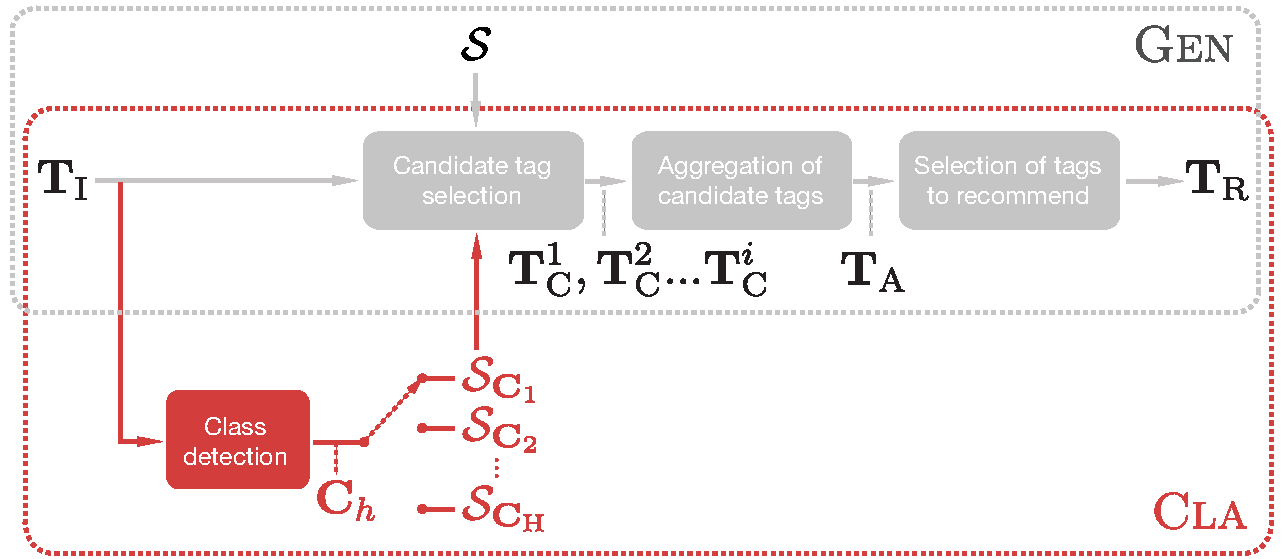
\includegraphics[width=1.0\columnwidth]{ch04_class/pics/fig_both_diagrams.pdf}
  \caption[Block diagram of the general and class-based tag recommendation methods]{Block diagram of the general (\textsc{Gen}) and class-based (\textsc{Cla}) tag recommendation methods.}
  \label{class:fig:diagrams}
\end{figure}

\begin{enumerate}
\item Candidate tag selection: Given a set of input tags $\inputTags$, this step uses a tag-tag similarity matrix $\similarityMatrix$ derived from the Freesound folksonomy to select a set of $\nCandidateTagsPerInputTag$ candidate tags $\candidateTagsPerInputTag$ for each input tag $\inputTag$. The tag-tag similarity matrix $\similarityMatrix$ is constructed by computing the association matrix $\associationMatrix = \left\{ \associationMatrixElement_{i,j} \right\}$, which represents the associations between tags and sounds in the Freesound folksonomy ($\associationMatrixElement_{i,j} = 1$ if sound $\audioClip_i$ is labeled with tag $\tagb_j$, and $\associationMatrixElement_{i,j} = 0$ otherwise). %Hence, $\associationMatrix$ is a sparse matrix that has as many columns as sounds in Freesound and as many rows as the set of distinct tags being used to label these sounds.%\footnote{In order to reduce the computational cost of the operations performed in this step and to get rid of potentially noisy tags, when building the association matrix we only consider tags whose frequency of occurrence is higher than a threshold $\tagFrequencyThreshold=10$ (i.e.,~we only consider tags that are used at least 10 times in the Freesound folksonomy). In this way the number of rows of the association matrix is reduced by $\approx$80\%, with only around $\approx$10\% of the associations between tags and sounds being actually ignored (Sec.~\ref{sec:general:datasets}).}. 
Given $\associationMatrix$, the tag-tag similarity matrix is obtained as $\similarityMatrix = \associationMatrixMultiplication'$, and we apply a simple normalisation to the elements $\left\{ \similarityMatrixElement_{\tagb_i,\tagb_j} \right\}$ of $\similarityMatrix$ so that $\similarityMatrixElement_{\tagb_i,\tagb_j}$ corresponds to the cosine similarity between tags $\tagb_i$ and $\tagb_j$ on the basis of their co-occurrence in sounds. Tags in $\candidateTagsPerInputTag$ are selected as the $\nCandidateTagsPerInputTag=100$ most similar tags to a given input tag $\inputTag$.

\item Aggregation of candidate tags: Given the sets $\candidateTagsPerInputTag$ from the first step, candidate tags are assigned a score $\scoreCandidateTag$ and aggregated into a single list of tags with scores $\aggregatedCandidateTags$. Such a score is determined by the candidate similarity-based ranking so that $\scoreCandidateTag=1$ for the most dissimilar candidate to a given input tag and $\scoreCandidateTag=\nCandidateTagsPerInputTag$ for the most similar one. The scores of tags that are present in different sets of candidates $\candidateTagsPerInputTag$ are added when aggregated in the final set $\aggregatedCandidateTags$.

\item Selection of tags to recommend: Considering the scores in $\aggregatedCandidateTags$, this step determines a threshold $\scoreThreshold$ to select the tags that are finally recommended. Here we use the strategy of determining the threshold $\scoreThreshold$ as a percentage of the maximum score in $\aggregatedCandidateTags$, and use a percentage parameter of $\percentageOfPercentageStrategy=0.15$ (Sec.~\ref{sec:general:percentage_strategy}). Tags in $\aggregatedCandidateTags$ are sorted by their score and those that satisfy $\scoreCandidateTag \geq \scoreThreshold$ are outputted as $\recommendedTags$, the final set of recommended tags.
\end{enumerate}

\subsection{Class-based tag recommendation}
\label{class:sec:class_based_tag_rec_ref}

The proposed class-based tag recommendation method is a variation of \textsc{Gen} based on the classification of the input tags $\inputTags$ into a set of $\nAudioClasses$ predefined audio classes\footnote{When referring to audio classes, we may use the terms ``class'' or ``category'' indistinctly.}. For every class $\audioClass$ ($\audioClass \in \audioClasses$, where $\audioClasses$ is the set of defined audio classes), a tag-tag similarity matrix $\similarityMatrixOfClassH$ is built in the same way as in the \textsc{Gen} method, except that in this case only the information of tag applications involving the sounds of the current class is considered (see below). As a result, a different tag-tag similarity matrix can be computed for every audio class, and the matrix $\similarityMatrixOfClassH$ that is used in the candidate tag selection step of the recommendation process depends on the classification of the input tags $\inputTags$ (Fig. \ref{class:fig:diagrams}).
Once the candidates are selected, the other two steps (Aggregation of candidate tags and Selection of tags to recommend) are computed in exactly the same way as in \textsc{Gen}.
We now describe the classification system that we use in the class detection step, and then explain the computation of the tag-tag similarity matrices.


\subsubsection{Classification system}
\label{class:sec:classification_system}

In order to classify a set of input tags $\inputTags$ of a sound $\resource$ into one of the audio classes, we make use of standard machine learning techniques. The structure of the classification system is very similar to what can be found in the existing literature on the classification of sound effects~\citep{Kuo1999,Casey2002,Sundaram2008,Roma2010}, musical instruments~\citep{Herrera2003,Livshin2003,Cano2004}, or music genre and mood~\citep{laurier2008,Bischoff2009,Chen2009,Tao2010}.
In these works, a set of low-level audio features is typically extracted from sounds in a given collection, yielding a feature vector representation of every sound. Also, sounds are manually annotated using the concepts of a taxonomy representing the particular classification domain (e.g.,~a taxonomy of musical instruments or sound effects). These taxonomies tend to be rather small, typically including less than 20 concepts. Then, supervised learning is performed using a classifier trained with the feature vectors corresponding to annotated sounds. 
%Some of these studies also make use of use of textual data such as lyrics and social tags at some point in the classification process but, to the best of our knowledge, no audio classification systems have been researched that only use information coming from tagging systems.

The classification we perform here only differs from this scheme in that we do not extract audio features from the sounds we classify, but use instead their existing associated tags (i.e.,~taglines) as feature vectors to train the classifier.
To do this, we follow a bag-of-words approach where each sound is represented as a vector whose elements indicate the presence or absence of a particular tag. 
Feature vectors contain all possible tags in the collection, thus their dimensionality is very high. 
Here we do not carry on any dimensionality reduction step to lower the size of the feature vectors. Instead, in order to keep them in manageable sizes, we apply the same threshold $\tagFrequencyThreshold=10$ described in Secs.~\ref{sec:general:datasets} and~\ref{class:sec:Gen}, removing all tags that are used less than 10 times.
The resulting feature vectors are very sparse, which makes the problem similar to what is normally found in text classification, where high dimensionality and sparseness are commonplace~\citep{Sebastiani2002}.
We experiment with a support vector machine (SVM) and a naive Bayes (NB) classifier, as these have been shown to be well suited for high dimensional and sparse classification tasks such as the one we are facing here~\citep{Bennett2000,Sebastiani2002}\footnote{We implement the classifiers using the  ``scikit-learn'' Python package (\url{http://scikit-learn.org}). We use the classes \texttt{LinearSVC} and \texttt{BernoulliNB} for SVM and NB, respectively, with default parameters. \texttt{LinearSVC} follows the ``one versus all'' approach for multiclass classification.}.
By not including extracted audio features in the classification system, we maintain a certain degree of generalisability for the class-based tag recommendation method, as the methodology remains applicable to other domains without further modifications. Nevertheless, what necessarily changes from domain to domain is the definition of classes.

\begin{table}
\ra{1.4}
\begin{center}
\footnotesize
\begin{tabular}{lp{9cm}}
\toprule
\multicolumn{1}{l}{\textbf{Class name}}	& \textbf{Description and examples} \\
\midrule
\textsc{SoundFX} & Sound effects (including \emph{foley}), footsteps, opening and closing doors, alarm sounds, cars passing by, animals and all kinds of noises or artificially created glitches.\\
\textsc{Soundscape} & Environmental recordings, street ambiances or artificially constructed complex soundscapes. \\
\textsc{Sample} & Instrument samples including single notes, chords and percussive hits (e.g.,~single notes of a piano recorded one by one and uploaded as different sounds, or samples from a complete drum set). \\
\textsc{Music} & Musical fragments such as melodies, chord progressions, and drum loops. This class is to \textsc{Sample} what \textsc{Soundscape} is to \textsc{SoundFX}. \\
\textsc{Voice} & Various voice-related sounds such as text reading, single words or recordings of text-to-speech processors. \\ 
\bottomrule
\end{tabular}
\end{center}
\caption[Name and descriptions of the audio classes]{Name and descriptions of the audio classes we defined.}
\label{tab:audio_classes}
\end{table}

Given the heterogeneity of the audio content in Freesound, we define the audio categories that we want to detect in a way that these can virtually include the whole range of sounds that can be found in Freesound.  
Hence, we define a total of $\nAudioClasses=5$ audio categories in which sounds can be classified. The resulting categories, shown in Table~\ref{tab:audio_classes}, are quite general and are in line with other sound categorisations reported in the literature~\citep{Casey2002, Roma2010}.
In order to create a dataset for the supervised learning process, we manually assigned one of the above categories to a number of sounds from Freesound. To do this, we followed an iterative process in which  we were presented with randomly chosen sounds from Freesound, and assigned them to one of the five categories. As it can be imagined, these categories are not completely orthogonal, and there were sounds for which the decision was not straightforward just by listening to the audio. In these cases, we also relied on provided textual descriptions of the sounds (i.e.,~their textual descriptions in Freesound). The crafted dataset includes a minimum of 2,088 sounds per category (corresponding to the case of \textsc{Speech}) and a maximum of 6,341 (for the case of \textsc{Samples}). Comparing the totality of Freesound sounds and the manually annotated subset, we observe qualitatively similar relative distributions of tag occurrences and number of tags per sound. 
Fig.~\ref{fig:tagclouds} shows the most commonly used tags for the five defined audio categories.
Using the manually crafted ground truth and the vector representations of sounds according to their taglines, we can train a classifier which, given a set of input tags $\inputTags$, can predict which category $\audioClass$ better fits the input.
In Sec.~\ref{class:sec:evaluation_classifier} we evaluate the classifier and report the results in terms of classification accuracy.

\begin{figure}
	\centering
		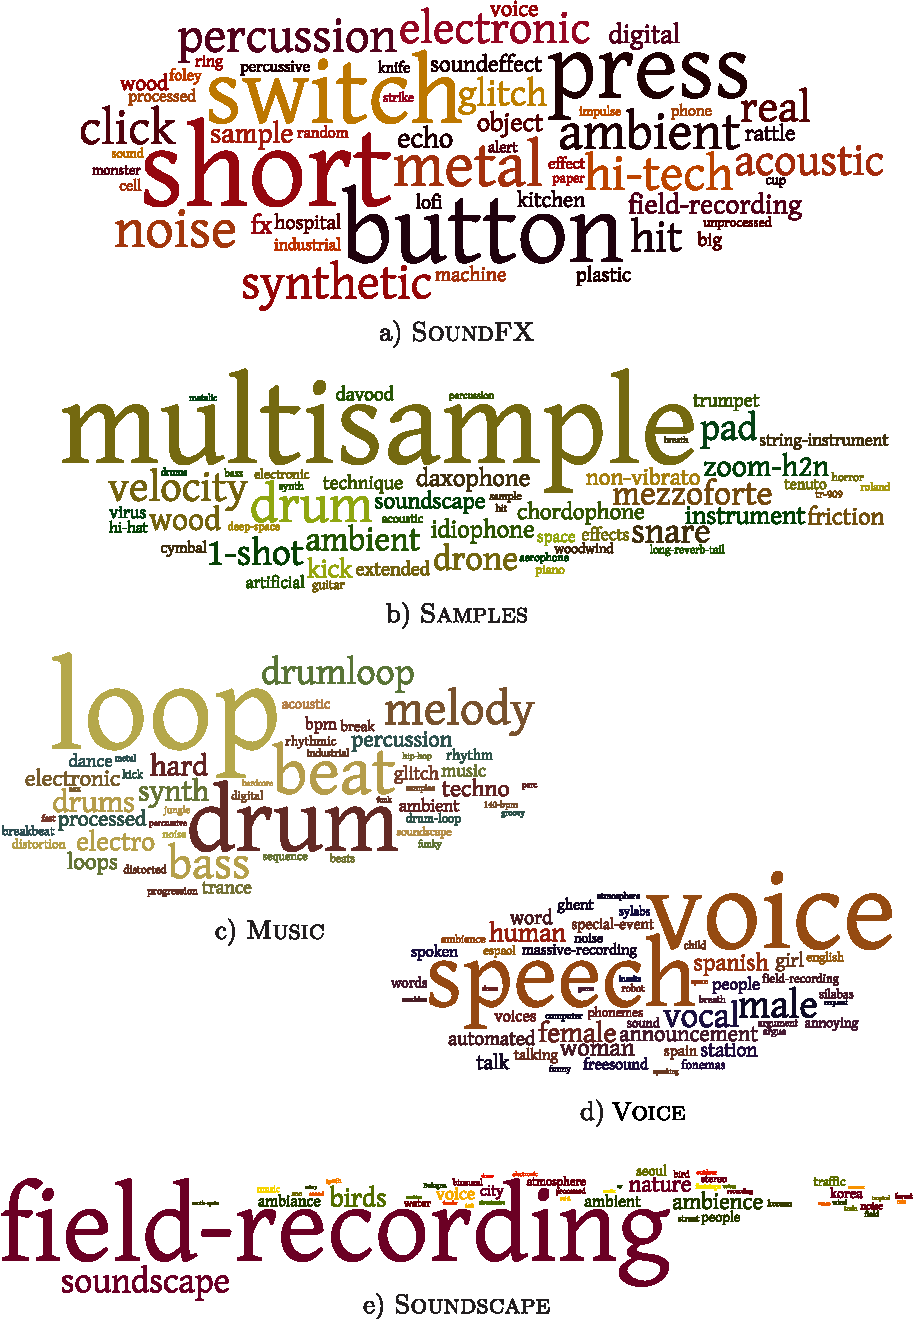
\includegraphics[width=0.95\columnwidth]{ch04_class/pics/tagclouds2.pdf}
	\caption[Tagclouds of the 50 most used tags in the five defined audio categories]{Tagclouds of the 50 most used tags in the five defined audio categories. The size of the tags is proportional to the frequency of occurrence among all sounds annotated under each category. For building these tagclouds, we only considered the set of sounds manually annotated as ground truth. Tagclouds were generated with the online tool available at \url{www.wordle.net}.}
	\label{fig:tagclouds}
\end{figure}


\subsubsection{Computation of tag-tag similarity matrices} 
\label{class:sec:similarity_matrix_computation}

As mentioned, the process of building the tag-tag similarity matrices $\similarityMatrixOfClassH$ is the same as the one for building $\similarityMatrix$, except that for every matrix $\similarityMatrixOfClassH$ we only consider information about tag applications from sounds belonging to $\audioClass$. 
For doing that, we reuse the classification system described above and classify all sounds of Freesound into one of the five audio classes, using as input tags the original taglines of the sounds in Freesound.  
Then, matrices $\similarityMatrixOfClassH$ can be built by only considering the columns of $\associationMatrix$ corresponding to the sounds of $\audioClass$. Hence, $\similarityMatrixOfClassH = \associationMatrixOfClassH\associationMatrixOfClassH'$, where $\associationMatrixOfClassH$ is a subset of $\associationMatrix$ in which the columns corresponding to sounds not in $\audioClass$ are removed.
Each matrix $\similarityMatrixOfClassH$ is normalised using the same process we use for $\similarityMatrix$ to obtain cosine similarity (Secs.~\ref{sec:general:step1} and~\ref{class:sec:Gen}). 

Notice that the similarity value between two tags $\tagb_i$ and $\tagb_j$ will be different in every matrix $\similarityMatrixOfClassH$ and in $\similarityMatrix$, with $\similarityMatrixOfClassH$ being tailored to the particular context of the $h$-th class. Note also that the number of distinct tags resulting from considering all sounds belonging to $\audioClass$ will be smaller than the total number of distinct tags resulting from considering all sounds from all classes (the size of the \emph{class vocabulary} will be smaller than the size of the \emph{general vocabulary}). Therefore, there will be some ``all-zeros'' rows in $\similarityMatrixOfClassH$, corresponding to the tags that are not used in the context of the particular class $\audioClass$. These tags are thus never recommended when using $\similarityMatrixOfClassH$.

\section[Results and evaluation of the classification system][Results and eval. of the classification system]{Results and evaluation of the classification system}
\label{class:sec:evaluation_classifier}

\subsection{Methodology}
\label{class:sec:evaluation_classifier_method}

To evaluate the classification system we follow a random sub-sampling cross-validation strategy where we split the aforementioned ground truth (i.e.,~the dataset) into training and testing sets. We then compute the out-of-sample accuracy as the percentage of well-classified instances from the testing set when using the fit from the training set. This process is repeated 100 times for each classifier and parameter configuration that we test (see below), and overall accuracy is obtained by averaging over the results of all repetitions. In each repetition, our dataset is composed of a random selection of 1,000 sounds from every category, adding up to a total of 5,000. This way we maintain a balance in the number of sounds per category. In addition, to avoid potential bias of our classifier to the tagging conventions of a particular user, we impose the limit of not getting more than 50 sounds of the same category uploaded by the same Freesound user. %We do that to avoid what could potentially be an equivalent of the \emph{album effect} that is known to happen in automatic music artist recognition~\citep{Whitman2001}. 
In each repetition, the testing set is selected as a random subset representing 10\% of the data, and being equally-distributed among categories (i.e.,~100 sounds per category). 

As mentioned in Sec.~\ref{class:sec:classification_system}, we test our method using SVM and NB classifiers. We also add a random classifier to serve as a baseline.
Given that for the class-based tag recommendation method the classification step is extensively used in situations with few input tags (i.e.,~when users start introducing tags), we are specially interested in evaluating the accuracy of the classification system in conditions of tag scarcity (i.e.,~low $|\inputTags|$).
Hence, we introduce a limitation to the testing set consisting of randomly removing tags from sounds prior to classification, only leaving a particular number of $N$ input tags per sound. We consider values of $N$ ranging from 1 to 5. This obviously adds another constraint to the selection of the testing set, which is to make sure that selected sounds have at least $N$ tags. The whole evaluation process is performed for all different values of $N$ and for both SVM and NB classifiers, yielding a total of 10 evaluated experiment combinations.

\subsection{Results}
\label{class:sec:evaluation_classifier_results}

\begin{figure}
	\centering
		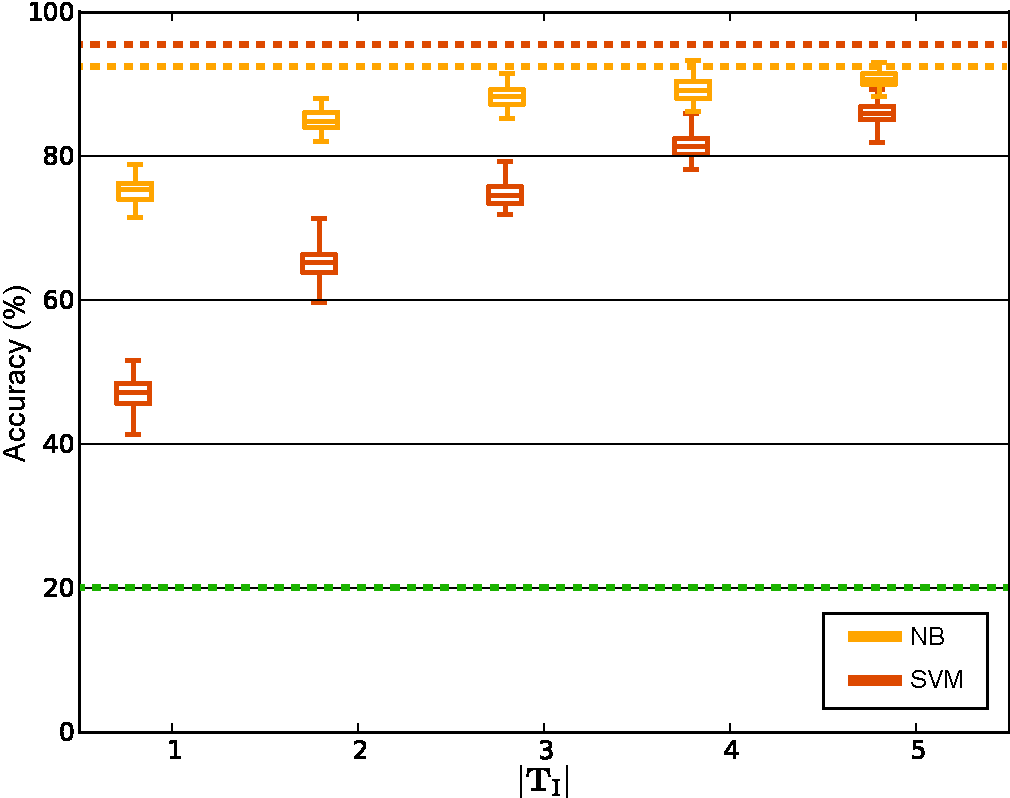
\includegraphics[width=\figSizeMid]{ch04_class/pics/classifier_results.pdf}
	\caption[Classification accuracy of the audio class detection step using SVM and NB classifiers]{Classification accuracy using SVM and NB classifiers. The dashed line at 20\% accuracy corresponds to the random baseline. The dashed lines around 95\% (SVM) and 90\% (NB) correspond to the accuracy achieved when no restriction on the number of tags for the testing set is performed, which can be considered as an upper bound limit.  
}
	\label{fig:classification_main_results}
\end{figure}

Fig.~\ref{fig:classification_main_results} shows the accuracies of our classification method for the experiment combinations described above. %(Sec.~\ref{class:sec:evaluation_classifier_method}). 
Note that all combinations are far above the random classifier accuracy of 20\%. The NB classifier reports overall a higher accuracy than the SVM, with a statistically significant average accuracy increase of 10\% ($p<10^{-12}$). Statistical significance is assessed by considering the maximum $p$-value across pairwise comparisons between experiment combinations and using the Wilcoxon signed-rank test with a significance level of 0.01~\citep{Corder2009}.
Overall, using the NB classifier, the classification system is able to successfully classify sounds among five generic categories inside the audio domain, with accuracies ranging from 75\% to 90\% depending on the number of input tags available for classification. 
As expected, the lowest accuracy is obtained when $|\inputTags| = 1$ (i.e.,~only one tag is given to the classifier). For $|\inputTags| \geq 4$, the classification accuracy reaches values close to 90\%. 

To complement these results, we performed additional experiments with different training set sizes (i.e.,~using less than than 90\% of sounds for training). The results we obtained are consistent with those reported above with little variation on accuracy for training set percentages higher than 50\%. This reinforces the validity of the classification results as the use of smaller training sets does not heavily affect classification accuracy. Furthermore, we also tested different values for the imposed maximum of 50 sounds uploaded by the same user in the same audio category. Our results show that the accuracy is not significantly influenced by such limit, thus asserting that the classifier is not biased to the tagging conventions of a particular user.% and questioning the existence of the aforementioned \textit{album effect} in our dataset. 
%\ref{class:sec:evaluation_classifier_method}


\section{Evaluation of the tag recommendation methods}
\label{class:sec:evaluation}

To evaluate the class-based tag recommendation method we designed an online experiment where participants had to tag a set of sounds from Freesound. 
The experiment was online for 15 days during June 2013, and was publicised in the Freesound front page. The goal of this experiment was twofold. 
First, we wanted to assess the usefulness of the \textsc{Cla} method with respect to the previous \textsc{Gen} method. 
Second, we wanted to get qualitative user feedback to better understand the strengths and weaknesses of the considered tag recommendation systems and, in a further stage, to understand the potential strengths and weaknesses of tag recommendation processes in general. 
%As mentioned in Sec.~\ref{sec:class:introduction}, this is yet an under-explored area.

Along with \textsc{Gen} and \textsc{Cla}, in the experiment we also evaluated two random variants of them, named \textsc{RGen} and \textsc{RCla}, respectively. These differ from the original variants in that, in the final step of the recommendation process, the set of recommended tags $\recommendedTags$ is replaced with an alternative set of the same length containing randomly selected tags either from the general vocabulary (\textsc{RGen}) or from the corresponding particular class vocabulary (\textsc{RCla}). Notice that the general vocabulary is always bigger than any of the individual classes' vocabulary. Hence, the random selection in \textsc{RGen} is performed over a bigger and more diverse pool of tags. Participants were not aware of the particular recommendation method underlying tag suggestions nor knew about the five audio classes in which we classify all annotated sounds. The dataset we used for the evaluation comprises Freesound data gathered between April 2005 and May 2012. % (Tables~\ref{tab:freesound_stats} and~\ref{tab:freesound_stats_sim_matrix}). 
Tables~\ref{tab:freesound_stats} and~\ref{tab:freesound_stats_sim_matrix} show basic statistics of the dataset and the resulting tag-tag similarity matrices that we built with this dataset.
%It includes tag applications which relate tags, sounds and users, and it is used to build the tag-tag similarity matrices $\similarityMatrix$ and $\similarityMatrixOfClassH$, as explained in Sec.~\ref{class:sec:similarity_matrix_computation}.
The online-experiment proceeded as follows:

\begin{table}
\begin{center}
\begin{threeparttable}
\ra{1.2}
\footnotesize
\begin{tabular}{p{8cm}r}
\toprule
\multicolumn{2}{c}{\textbf{Freesound dataset}} \\
\midrule
Number of sounds & 140,622  \\ 
Number of unique tags\tnote{a}  & 43,696  \\ 
Number of contributor users\tnote{b}  & 6,948  \\ 
Number of tag applications & 990,574  \\ 
Average tags per sound (tagline length) & 7.04  \\
\bottomrule
\end{tabular}
\begin{tablenotes}
    \item[a] Not necessarily semantically unique.
    \item[b] Users that have contributed by uploading, at least, one resource.
    \end{tablenotes}
  \caption[Basic statistics of the Freesound dataset]{Basic statistics of the Freesound dataset (including data collected between April 2005 and May 2012).}
\label{tab:freesound_stats}
\end{threeparttable}
\end{center}
\end{table}

\begin{table}
\ra{1.2}
\footnotesize
  \begin{center}
\begin{tabular}{lcc}
\toprule
\multicolumn{3}{c}{\textbf{Tag-tag similarity matrices}} \\  
& \textbf{Num. sounds} & \textbf{Vocabulary size} \\ 
\midrule

General matrix ($\similarityMatrix$) & 140,622 & 7,710 \\ 
Matrix for class \textsc{SoundFX} & 29,725 & 4,584 \\
Matrix for class \textsc{Soundscape} & 38,001 & 5,768 \\ 
Matrix for class \textsc{Sample} & 26,452 & 3,280 \\ 
Matrix for class \textsc{Music} & 34,139 & 4,303 \\ 
Matrix for class \textsc{Voice} & 15,305 & 3,557 \\
\bottomrule
\end{tabular}
  \caption[Basic statistics of the tag-tag similarity matrices]{Basic statistics of the resulting tag-tag similarity matrices.}
\label{tab:freesound_stats_sim_matrix}
  \end{center}
\end{table}


\begin{description}
  \item \textbf{Instructions page}: First, participants were presented with an introduction page displaying detailed instructions for the experiment (Fig.~\ref{class:fig:ss0_introduction}). Participants were told they would have to annotate 20 sounds from Freesound, using as many tags as they felt appropriate for every sound (we suggested participants to use five or more tags, but it was not mandatory). Participants were also told that as soon as they started typing tags, a list of tag suggestions would appear and that they could choose tags from this list if they felt the suggestions were appropriate. We also recommended participants to use headphones for better listening conditions.

\begin{figure}
  \centering
  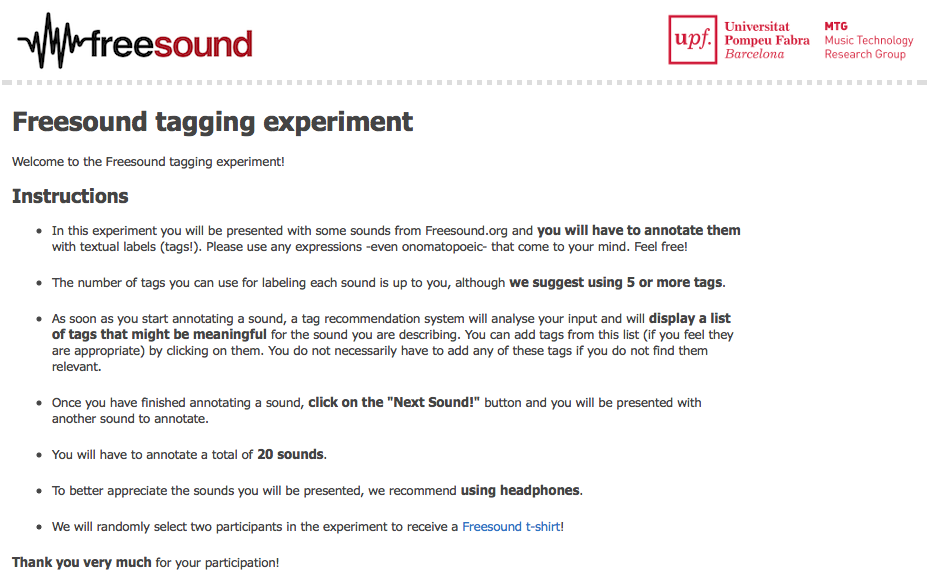
\includegraphics[width=1.0\columnwidth]{ch04_class/pics/fig_ss0_instructions.png}
  \caption[Screenshot of the instructions page]{Screenshot of the instructions page.}
  \label{class:fig:ss0_introduction}
\end{figure}

  \begin{figure}
  \centering
  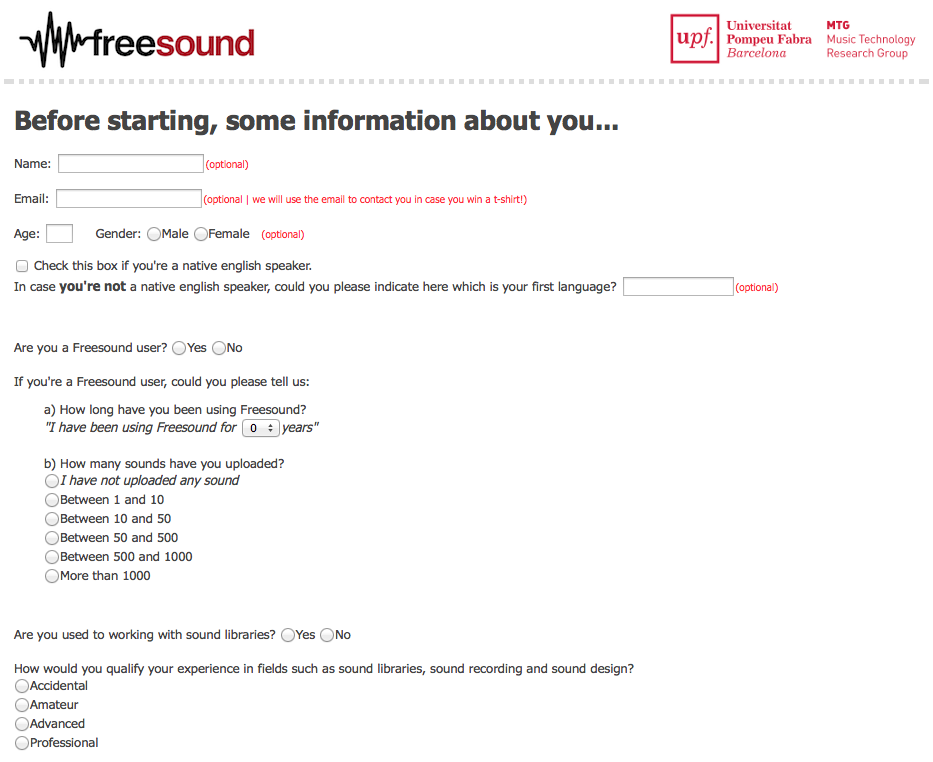
\includegraphics[width=1.0\columnwidth]{ch04_class/pics/fig_ss1_questionnaire.png}
  \caption[Screenshot of the questionnaire page]{Screenshot of the questionnaire page.}
  \label{class:fig:ss1_questionnaire}
\end{figure}

   \begin{figure}
  \centering
  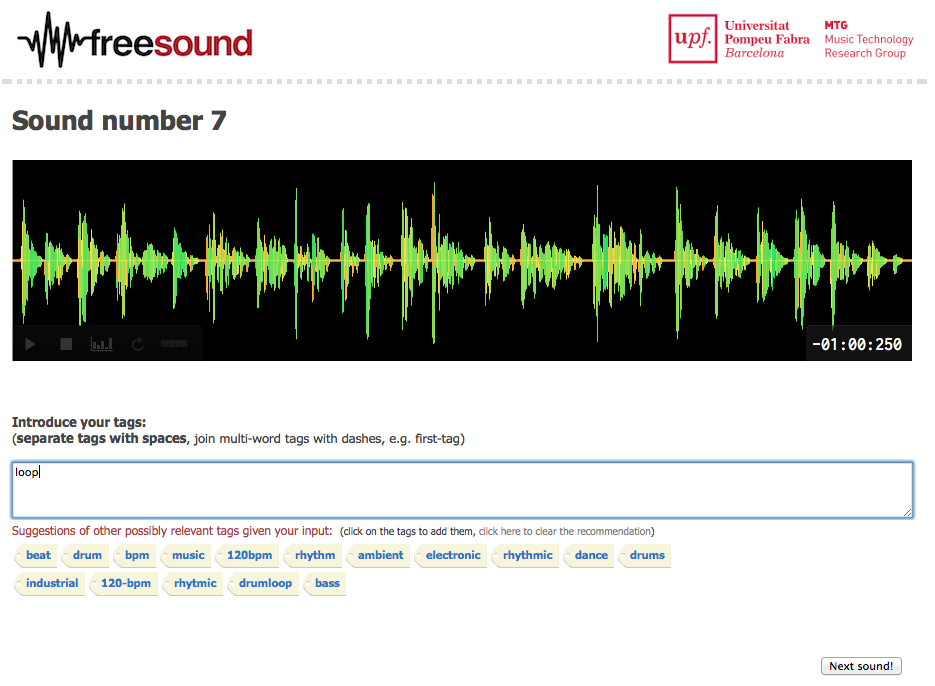
\includegraphics[width=1.0\columnwidth]{ch04_class/pics/fig_ss2_sound.png}
  \caption[Screenshot of the sound annotation page]{Screenshot of the sound annotation page.}
  \label{class:fig:ss2_sound}
\end{figure}

  \item \textbf{Questionnaire}: After the introduction, a short questionnaire (Fig.~\ref{class:fig:ss1_questionnaire}) was presented to collect some basic user data and information about their experience in working with sound libraries, their experience using Freesound (including the number of uploaded sounds) and their native language (in particular to be able to differentiate between native and non-native English speakers).

  \item \textbf{Sound annotation}: Once the questionnaire was completed, participants started annotating sounds. From the ground truth we defined when designing the recommendation system (Sec.~\ref{class:sec:classification_system}), we manually selected 50 sounds per class\footnote{The sounds we selected for the annotation phase of the online experiment (a total of 250, 50 per class) were removed from the ground truth and thus were not used to train the classifier described in section \ref{class:sec:classification_system}.}. These sounds were selected trying to cover a certain variety of sounds and avoiding those that would presumably be very hard to annotate. From this pool of 250 sounds, every participant was assigned a random selection of four sounds per class. Then, each of the four sounds was assigned a different tag recommendation method that would be used when the participant annotated the sound. In this way, every participant was assigned a total 20 sounds, equally distributed among audio classes and recommendation methods. Participants were presented with the first sound and had to annotate it by typing tags in a text box. The sound could be reproduced using a web player that also showed a visualisation of the waveform and the spectrogram of the sound (Fig.~\ref{class:fig:ss2_sound}). As soon as the participant started typing, a list of suggested tags appeared below the text box. This list was computed using the tag recommendation method assigned to the currently annotated sound, and was being updated every time a new tag was written in the text box. Similar to the Freesound upload system, tags had to be separated by spaces and multi-words joined with hyphens. Hence, the recommendation was primarily updated every time a blank space was introduced. Users could click over the tags shown in the list to automatically append them in the text box (Fig.~\ref{class:fig:ss2_sound}). Once a participant considered a sound was fully annotated, she could click on the ``Next sound'' button and be presented with the following sound. Participants were also provided an URL that they could save for later resuming the experiment in case they did not want to annotate all sounds in one go. Noticeably, we logged information about all the keystrokes and mouse clicks that participants performed with the corresponding timestamps.

  \item \textbf{Feedback page}: After annotating the 20 sounds, participants were presented with a page thanking their participation and offering some space in a text box to give some feedback about the experiment. Alternatively, they were also offered to write the feedback in a particular thread of the Freesound forums.

\end{description}

Considering the logs gathered during the experiment, we define a simple measure for evaluating the ``usefulness'' of every tag recommendation method in the tagging process. The measure consists of counting, for every set of tags assigned to a sound by a particular participant, the number of these tags that were recommended by the system during the annotation process (i.e.,~the number of recommended tags that were \emph{correctly predicted} by the system or, what is the same, \emph{accepted} by the participant). Then, this number can be averaged over all sounds annotated with each recommendation method, and obtain in this way a general characterisation of the method.
Let $\resources$ be a set of resources, let $\tagsOfSoundR$ be the set of tags that a participant used to annotate a particular sound $\resource$, and let $\nthRecommendedTagsInSession$ be one of the sets of recommended tags that were presented to the user in the successive $\numberOfTagRecommendationsInSession$ tag recommendations during the tagging process of that particular sound $\resource$. Then, we can define $\nAcceptedTags$, the number of correctly predicted tags (or accepted tags), as
\begin{equation}
\nAcceptedTags = \frac{1}{|\resources|} \sum\limits_{\resource\in \resources}{\left\vert \tagsOfSoundR \cap \left( \bigcup^{\numberOfTagRecommendationsInSession}_{\recommendationsInSessionIndex=1} \nthRecommendedTagsInSession \right) \right\vert} .
\label{class:eq:n_accepted_tags}
\end{equation}
Notice that $\nAcceptedTags$ is roughly equivalent to a standard recall measure (without the normalization term). We employ this measure instead of standard precision and recall (e.g.,~as done in~\citeauthor{Jaschke2009}~\citeyear{Jaschke2009}) because the nature of our evaluation has some particularities which make such metrics less useful. As described above, several tag recommendations are performed during the annotation of a single sound (i.e.,~every time that a new tag is introduced the recommendation is recomputed). As a result, the total number of recommended tags for every sound is much larger than the final number of assigned tags. If we computed precision and recall by comparing the whole set of recommended tags for every sound with the final taglines assigned by users, we would obtain very low precision values which, in our opinion, are not as representative as $\nAcceptedTags$. In our evaluation (and in a real-world tag recommendation scenario), users are the ones who finally decide which of the recommended tags are relevant for a particular resource. Therefore, the length of the recommendation is not as important as the fact that it contains meaningful suggestions (i.e.,~recall is arguably more important than precision).


\section{Results of the tag recommendation methods}
\label{class:sec:results}

During the two weeks the experiment was online, we gathered a total 201 experiment logs from 190 unique participants (a few participants decided to repeat the experiment more than once). Among all these experiment logs, 80 correspond to unfinished experiments (i.e.,~with less than 20 sounds annotated) which we do not consider in the analysis. In addition, we apply a filter to discard logs from experiments that were finished very quickly and with very few calls to the recommendation methods. More specifically, we discard logs from experiments completed in less than 10 minutes (average of 30 seconds per sound) and from experiments not reporting a minimum of three calls to the recommendation system for every annotated sound. We discard these logs as we consider that participants did not pay enough attention when annotating sounds and thus contain potentially noisy data. After filtering, we are left with 70 logs that we consider as sufficiently reliable data for analysis. In the following sections we report the results of the different aspects of the online experiment that we analyse.

\subsection{Correctly predicted tags per recommendation method}
\label{class:sec:accepted_tags_results}

First, we report the basic accuracy of the considered tag recommendation methods (Table~\ref{tab:results_general_ub}, leftmost column).
We observe that random methods \textsc{RCla} and \textsc{RGen} report considerably lower average $\nAcceptedTags$ than \textsc{Cla} and \textsc{Gen}. Thus, our methods generate much more meaningful recommendations than the random baselines. Interestingly, we also observe that both class-based methods \textsc{Cla} and \textsc{RCla} report higher averages than their general counterparts \textsc{Gen} and \textsc{RGen}. This suggests that tag recommendations improve when using class-based methods. However, the differences are found not to be statistically significant. In the following comparisons, and if not stated otherwise, statistical significance is assessed by performing pairwise comparisons using the Mann-Whitney U test with a significance level of 0.05~\citep{Corder2009}. 

\begin{table}
\ra{1.2}
\footnotesize
  \begin{center}
\footnotesize
\begin{tabular}{lc@{\hskip 0.65cm}cc@{\hskip 0.65cm}cc}
\toprule
	 %& \multicolumn{5}{c}{\textbf{Average number of correctly predicted tags}} \\
	 &  \textbf{All} & \textbf{Expert} & \textbf{Non-expert} & \textbf{Native} & \textbf{Non-native} \\ 
	 \midrule
 	\textsc{Cla} 	& 2.414 (2.775) 	&  2.547 (2.988) 	&  2.179 (2.224) 	&  2.950 (3.382) &  1.963 (2.027) \\ 
	\textsc{Gen} 	& 2.154 (2.526) 	&  2.163 (2.663)	&  2.147 (2.229) 	&  2.656 (3.006) &  1.732 (1.938) \\ 
	\textsc{RCla} 	& 0.260 (0.671) 	&  0.278 (0.680) 	&  0.211 (0.663) 	&  0.300 (0.705) &  0.226 (0.638) \\ 
	\textsc{RGen} 	& 0.166 (0.455) 	&  0.139 (0.458) 	&  0.253 (0.458) 	&  0.194 (0.518) &  0.142 (0.392) \\
	\bottomrule
\end{tabular}
\end{center}
\caption[Average number of correctly predicted tags per recommendation method]{Average number of correctly predicted tags $\nAcceptedTags$ (standard deviation in parenthesis) of the user-based evaluation approach for the different groups of participants.}
\label{tab:results_general_ub}
\end{table}

Next, we repeat the same analysis but considering different groups of experiment logs according to the questionnaire that participants had to fill at the beginning of the experiment (Table~\ref{tab:results_general_ub}). In particular, we compute $\nAcceptedTags$ for each recommendation method considering groups of logs corresponding to experienced participants (i.e.,~participants that checked the box marked with the question ``Are you used to working with sound libraries?'' in the questionnaire; second column in Table~\ref{tab:results_general_ub}), non-experienced participants (third column),  native English speakers (fourth column), and non-native speakers (fifth column). We again observe that \textsc{Cla} reports higher averages than \textsc{Gen}, which further supports the idea that class-based recommendations bring some improvements over the general method. Interestingly, in the case of experienced participants, the difference between \textsc{Cla} and \textsc{Gen} increases with respect to the same comparison when considering all participants. In this case we get a statistically significant increase of 0.38 ($\pvalue < 2.91\cdot 10^{-2}$). Furthermore, the difference between \textsc{RCla} and \textsc{RGen} also increases for the expert group (with respect to all participants) and becomes statistically significant ($\pvalue < 2.47\cdot 10^{-3}$). This suggests that expert participants clearly appreciate a difference between \textsc{Cla} and \textsc{Gen} methods (even for the random versions) and find class-based recommenders to be more useful. On the other hand, we observe that when analysing the non-experienced participants group, the differences between class-based and general methods gets blurred, with almost no difference between the two types of recommendation methods. Thus, non-experienced participants are not able to tell the difference between class-based and general recommendations. Overall, these results indicate that the usefulness of class-based tag recommendations compared to general recommendations is slightly higher, especially prominent in the case of experienced participants.

Considering the last two groups of participants (native and non-native English speakers), we observe that the differences between class-based and general recommendation systems are quite similar to those obtained when considering all participants. Class-based systems report higher $\nAcceptedTags$, but the increments are practically the same for both native and non-native groups (there is no statistically significant difference between the increments). Thus, we do not see a direct general implication of language in method preference. Nevertheless, there is a significant difference in the absolute number of correctly predicted tags among the native and non-native participant groups (Table~\ref{tab:results_general_ub}). Native English speakers tend to accept an average of 0.96 tags more than non-native ones ($\pvalue = 4.61\cdot 10^{-3}$). Furthermore, we observe that native English speaking participants tend to annotate sounds with an average of 0.32 tags more than non-native ones ($\pvalue = 3.24\cdot 10^{-6}$). This suggests that, in these experiments, native speakers use more tags for describing sounds than non-native speakers, and tend to accept more recommendations.  
%To the best of our knowledge, this is the first time evidence is reported with regard to the comparison of native's and non-native's tagging behaviour. 
%Our results suggest that native speakers use more tags when describing online resources than non-native participants. 
%Hence, this is an interesting aspect that should not be overlooked in future user-based evaluations and studies involving user participation. 
Overall, we see that both native and non-native speakers prefer \textsc{Cla} over \textsc{Gen} (and \textsc{RCla} over \textsc{RGen}), but that this preference is not stronger than in any of the other user groups.

\subsection{Correctly predicted tags per audio class}
\label{class:sec:accepted_tags_audio_class_results}

To gain insight into how recommendation methods work for the different audio classes defined above (Table~\ref{tab:audio_classes}), we group annotated sounds by their class and recommendation method, and computed the average number of correctly predicted tags $\nAcceptedTags$ for each group (Fig.~\ref{class:fig:accepted_tags_per_category_per_method}). In general, sounds under \textsc{Soundscape} and \textsc{Voice} classes report higher $\nAcceptedTags$ than sounds under the other classes. This is probably because there are some tags such as \texttt{field-recording}, \texttt{nature} or \texttt{voice} which are very common in these classes and are very generic (i.e.,~could be used to annotate almost any sound in \textsc{Soundscape} or \textsc{Voice} classes). 

\begin{figure}
  \centering
  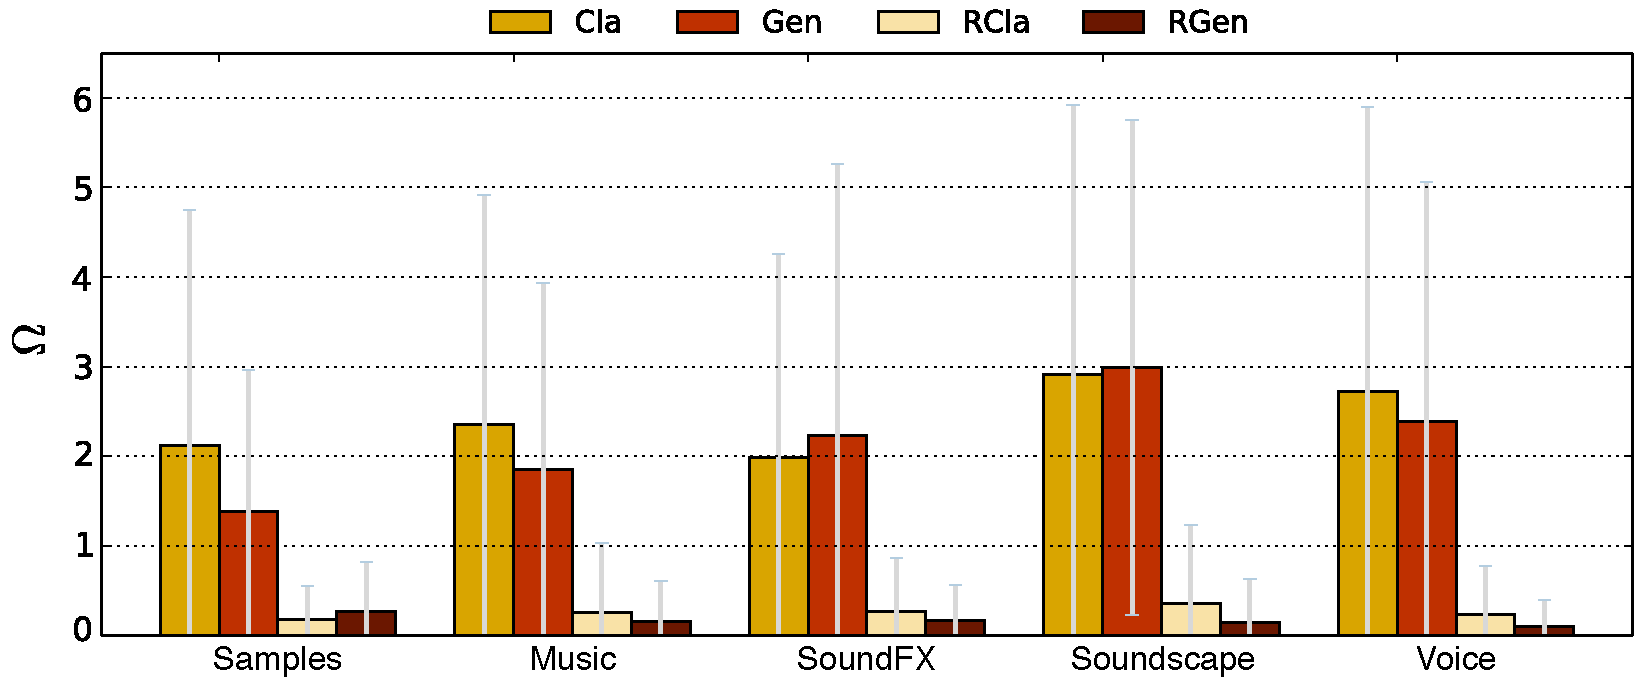
\includegraphics[width=0.85\textwidth]{ch04_class/pics/fig_AT_per_sound_category_per_method.pdf}
  \caption[Average number of correctly predicted tags per audio class and recommendation method]{Average number of correctly predicted tags $\nAcceptedTags$ per audio class and recommendation method.}
  \label{class:fig:accepted_tags_per_category_per_method}
\end{figure}

It can also be observed that not all audio classes feature higher $\nAcceptedTags$ for the \textsc{Cla} method when compared to the \textsc{Gen} method. \textsc{Soundscape} sounds report higher $\nAcceptedTags$ for \textsc{Gen} than for \textsc{Cla}, although the difference of 0.07 is not statistically significant ($\pvalue = 4.56\cdot 10^{-1}$). \textsc{SoundFX} sounds also report higher $\nAcceptedTags$ for the \textsc{Gen} method and, although the difference is still not statistically significant ($\pvalue = 3.80\cdot 10^{-1}$), the increase of 0.25 is this time larger. \textsc{Sample}, \textsc{Music} and \textsc{Voice} classes report higher $\nAcceptedTags$ for \textsc{Cla} recommendations, with larger $\nAcceptedTags$ increases and closer to statistical significance. This suggests that the adaptation to audio categories that the \textsc{Cla} method performs is better exploited in \textsc{Voice}, \textsc{Music} and \textsc{Sample} classes than in \textsc{Soundscape} or \textsc{SoundFX}. We hypothesise that the vocabulary needed to accurately describe sounds from the former classes is more reduced than the vocabulary needed for other sounds. 
Therefore, the class-based method can easily adapt to the class context and produce better recommendations.
These recommendations probably include tags which have a narrower semantic meaning than the tags recommended with the general method.
On the other hand, sounds under \textsc{Soundscape} and \textsc{SoundFX} classes cover a wider range of sounds and need a larger vocabulary to be well-described. In this situation, the \textsc{Cla} method does not adapt well and does not improve the  \textsc{Gen} results. Our hypothesis is partially supported by looking at the actual size of the resulting class vocabularies after computing the tag-tag similarity matrix per class ($\similarityMatrixOfClassH$, Table~\ref{tab:freesound_stats_sim_matrix}). \textsc{Voice}, \textsc{Music} and \textsc{Sample} produce smaller similarity matrices, with less tags in the vocabulary, than \textsc{Soundscape} and \textsc{SoundFX}.

\subsection{Correlation between number of uploaded sounds and the number of correctly predicted tags}
\label{class:sec:n_uploaded_sounds_at_correlation}

All participants in our experiment were Freesound users. However, not all of them had experience in uploading and tagging sounds in Freesound. In order to get some insight in how being used to tagging sounds affects $\nAcceptedTags$, we compute the correlation between the number of uploaded sounds and the number of accepted tags, grouping sounds into the four evaluated recommendation methods (Table~\ref{tab:correlation_uploaded_sounds_at}). To measure that correlation, we employ the Spearman's rank correlation coefficient~\citep{Corder2009}, with $\spearmanCorrelationCoefficient$ denoting the correlation coefficient and $\pvalue$ the $\pvalue$-value associated with it.

We find the strongest correlation for the \textsc{Cla} method ($\spearmanCorrelationCoefficient=0.276$, $\pvalue<3.76\cdot 10^{-7}$). Thus, in this case, $\nAcceptedTags$ tends to grow along with the number of uploaded sounds. A less significant correlation is reported for the \textsc{Gen} method ($\spearmanCorrelationCoefficient=0.105$, $\pvalue<5.61\cdot 10^{-3}$). \textsc{RCla} and \textsc{RGen} present no significant correlations ($\spearmanCorrelationCoefficient=0.087$, $\pvalue<1.13\cdot 10^{-1}$ and $\spearmanCorrelationCoefficient=0.063$, $\pvalue<2.55\cdot 10^{-1}$, respectively). This finding suggests that the more familiar the participants are with the Freesound uploading and tagging processes, the more recommended tags they tend to accept, especially when recommendations are generated with the \textsc{Cla} method. This result is consistent with the previous observation that experienced participants tend to accept more tags than non-experienced ones when recommendations are generated by \textsc{Cla} (Sec.~\ref{class:sec:accepted_tags_results}). Again, we are not aware of any study considering user familiarity in the context of resource tagging. Therefore, our results represent a novel and original contribution with regard to this aspect.
% the rank correlation coefficient was previously cited as hogg1995

\begin{table}
\ra{1.2}
\footnotesize
  \begin{center}
\footnotesize
\begin{tabular}{l@{\hskip 1.0cm}cccc}
	\toprule
	 %&  \multicolumn{4}{c}{\textbf{Average number of correctly predicted tags}}  \\
	 \textbf{Num. of uploaded sounds}	&  \textsc{Cla} & \textsc{Gen} & \textsc{RCla} & \textsc{RGem}  \\ 
	 \midrule
	  0 & 2.105 & 2.036 & 0.221 & 0.126 \\
	  1 to 10 & 1.823 & 2.027 & 0.293 & 0.133 \\
	  11 to 50 & 2.580 & 1.820 & 0.220 & 0.240 \\
	  51 to 500 & 2.289 & 2.222 & 0.311 & 0.133 \\
	  501 to 1000 & 4.160 & 2.035 & 0.380 & 0.300 \\ 
	  \bottomrule

\end{tabular}
\end{center}
\caption[Average number of correctly predicted tags per number of uploaded sounds and recommendation method]{Average number of correctly predicted tags $\nAcceptedTags$ per number of uploaded sounds and recommendation method. The ranges in the number of uploaded sounds are determined by the questionnaire that participants had to fill at the beginning of the experiment (Fig.~\ref{class:fig:ss1_questionnaire}).}
\label{tab:correlation_uploaded_sounds_at}
\end{table}


\subsection{Timing aspects}
\label{class:sec:timing_results}

Timing is also an often unconsidered aspect when evaluating tag recommendation systems. However, it is interesting because it can reveal some insights about the annotation process. In our experiments, we measured the average time invested for annotating a sound and observed that there exists a significant correlation between the length of the sounds and the time invested to annotate them, shorter sounds being the fastest to be annotated ($\spearmanCorrelationCoefficient=0.24$, $\pvalue<5.68\cdot 10^{-19}$). This could be expected, as shorter sounds tend to be less complex and need less time for listening to them. Consistently, sounds belonging to the \textsc{Soundscape} class need an average of 15 extra seconds to be described when compared to sounds belonging to other classes ($\pvalue< 8.12\cdot 10^{-3}$). On the other hand, \textsc{Sample} sounds need less time than the rest ($\pvalue < 3.15\cdot 10^{-2}$). This can be explained because \textsc{Soundscape} sounds are generally longer than sounds from other classes, while \textsc{Sample} sounds 
tend to be shorter. Nevertheless, when comparing the four different recommendation methods, we have not observed any statistically significant differences in the average time invested for annotating sounds. Therefore, in our particular comparison, the choice of a recommendation method does not seem to affect the time needed to annotate sounds.

\subsection{User feedback}
\label{class:sec:user_feedback}

In the last phase of the online experiment, participants were provided the opportunity to give some feedback in the form of textual comments (Sec.~\ref{class:sec:evaluation}). Looking at these comments, we observe some recurring opinions that,  if extrapolated, bring also valuable insights into recommendation processes in general. First of all, participants agree in that the process of annotating sounds (and by extension the process of recommending tags) is a very hard task, and that recommendations are a generally useful tool but not always needed or used. In fact, approximately 29\% of all tag annotations performed during the experiment were suggested by the recommendation systems\footnote{This percentage is computed without taking into account tag recommendations performed with random methods, which obviously did not provide meaningful recommendations.} (i.e.,~were correctly predicted), but the other tags were created by users.

A lot of participants point out that annotation is especially hard when the sound being described is not recorded/created by the person annotating it (which was always the case in our experiment). In these cases, there is a lot of meaningful information about the sound which most of the times can not be determined without the knowledge of how the sound was created (e.g.,~software used, recording device, location of a recording, etc.). Some participants also point out that in order to perfectly annotate musical sounds such as drum loops or instrument notes, a lot of time needs to be invested in determining properties such as beats per minute or the pitch of a note. These issues are particularly relevant in our context, where participants had to annotate sounds not created by themselves. Finally, another repeated comment is that tag suggestions are more useful for ``nature'' and ``human-related'' sounds, whereas ``abstract'' and ``synthetic'' sounds require more tags to be manually introduced 
before some meaningful suggestions are made. These comments are somehow aligned with the results reported in Fig.~\ref{class:fig:accepted_tags_per_category_per_method}, where we see that \textsc{Soundscape} and \textsc{Voice} classes are the ones that report higher $\nAcceptedTags$.


\subsection{Tag analysis}
\label{class:sec:tag_examples}

Here we have a closer look at the experiment logs in order to get some insight into the type of tags that are recommended and in which cases these are correctly predicted. We observe several interesting patterns that we believe also help comprehend in more detail tag recommendation processes in general. First of all, there are some tags which are recommended and accepted many times in the online experiment. These tags correspond to very generic concepts such as \texttt{field-recording}, \texttt{voice}, \texttt{electronic}, \texttt{loop}, \texttt{nature} or \texttt{percussion}. These recommendations are useful in providing some kind of general categorization to annotated sounds, but sounds only tagged with these kind of tags do clearly lack specificity in the annotations. We observe that another recommendation pattern consists of tags that are suggested many times but are rarely accepted. This is the case of tags such as \texttt{sound} or \texttt{recording}, for which we hypothesise that the meaning is too obvious to be considered as relevant information for participants. This is also the case of tags like \texttt{soundscape}, \texttt{percussion-loop}, \texttt{drum-loop} or \texttt{natural-reverb}, which can typically be represented with alternative tags, compound-tags or pairs of tags such as \texttt{field-recording} (instead of \texttt{soundscape}), \texttt{loop}, \texttt{percussion}, \texttt{drum}, \texttt{natural} or \texttt{reverb}.

We also observe that there are some tags whose low acceptance can be explained because of its subjective meaning (e.g.,~\texttt{groovy}, \texttt{threatening}) or because participants can not assess its correctness because they are not the authors of the annotated sounds (e.g.,~\texttt{multi-sample}, \texttt{improvised}). Obviously there are also some suggested tags which are not accepted because they are simply not appropriate for the sounds being described. This is the case of tags like \texttt{piano}, \texttt{guitar} or \texttt{pad}, which are sometimes recommended to sounds that clearly do not contain piano, guitar or pad-like sounds. Finally, we observe a last group of suggestions which correspond to tags not usually suggested but normally accepted such as \texttt{annoucement}, \texttt{syn\-the\-sizer}, \texttt{footsteps} or \texttt{airplane}. We consider these as being very good recommendations as they correspond to not-so-general concepts and are apparently recommended only when they are needed. Overall, recommendations provided by our methods tend to be useful when recommending general tags, referring to concepts that can be used as a broad categorisations of the sounds. However, recommendations are not as useful when they refer to more detailed aspects of the sounds being annotated.


\section[Complementary results and evaluation of the tag recommendation methods][Comp. res. and eval. of the tag rec. methods]{Complementary results and evaluation of the tag recommendation methods}
\label{class:sec:pb_evaluation}

In order to complement the user-based evaluation, we also consider a systematic assessment of the different tag recommendation methods (\textsc{Cla}, \textsc{Gen}, \textsc{RCla} and \textsc{RGen}) following the methodology we described in Chapter~\ref{sec:general}. This complementary assessment follows a setup based on a tag prediction task which we now describe.

\subsection{Methodology}

For this evaluation we consider sounds and annotations of the same Freesound dataset described in Sec.~\ref{class:sec:evaluation}. 
The process we follow is very similar to that described in Chapter~\ref{sec:general} (Sec.~\ref{sec:general:evaluation_methodology_a}).
However, for each fold of the 10-fold cross-validation, we now have to follow two extra steps to set up the system for producing tag recommendations.
The first step consists of training a classifier that allows the classification of the input tags into one of the five defined audio classes. We train the classifier as described in Sec.~\ref{class:sec:classification_system}, but feeding the classifier only with these sounds that are present both in the training set of the current fold and in the ground truth we built when designing the system (i.e.,~we only use sounds from the training set that we know to which audio category they belong to).

The second step of the training phase consists of building the general tag-tag similarity matrix $\similarityMatrix$ and the matrices $\similarityMatrixOfClassH$ for every class $\audioClass$. For this we use information from all the sounds in the training set. Notice that building $\similarityMatrixOfClassH$ requires the classification of all sounds of the training set into one of the five defined categories (Sec.~\ref{class:sec:similarity_matrix_computation}). We perform that classification using the same classifier trained in the first step of the training phase. Hence, this classifier is not only used during the recommendation process to automatically detect the audio class of a set of input tags $\inputTags$, but it is also used to build the different tag-tag similarity-matrices $\similarityMatrixOfClassH$ corresponding to each audio class.

Similarly to Sec.~\ref{class:sec:classification_system}, after the training phase we pick every sound in the evaluation set and randomly delete a set of tags $\deletedTags$ from its originally assigned tags, yielding $\inputTags$, the input to our recommendation system. The number of tags we delete is chosen uniformly at random, with only the constraint of leaving a minimum number of input tags of $|\inputTags| \geq 3$ so that there is presumably enough information for the recommender systems to provide good recommendations (see Sec.~\ref{sec:general:datasets}). This constraint also implies that, in order to be able to remove at least one tag for each sound ($|\deletedTags| \geq 1$), we can only consider for evaluation the sounds that have at least four tags\footnote{This filtering is done before the whole evaluation process starts, therefore we evaluate the same number of sounds in each fold.}. After we remove some tags, we run the four tag recommendation methods using $\inputTags$ as input and the similarity matrices we computed in the training phase. 
%As evaluation measures we compute standard precision ($\precision_\audioClipEvaluatedInComplementaryEvaluation$), recall ($\recall_\audioClipEvaluatedInComplementaryEvaluation$), and f-measure ($\fmeasure_\audioClipEvaluatedInComplementaryEvaluation$) for each individual sound $\audioClipEvaluatedInComplementaryEvaluation$ according to
As evaluation measures we compute standard precision, recall, and f-measure ($\precision$, $\recall$, and $\fmeasure$, respectively) for each evaluated sound (Eq.~\ref{eq:prf_ch2}).
%\begin{equation*}
%\precision_\audioClipEvaluatedInComplementaryEvaluation = \frac{|\recommendedTags \cap \deletedTags|}{|\recommendedTags|} \text{ }, \text{ }
%\recall_\audioClipEvaluatedInComplementaryEvaluation = \frac{|\recommendedTags \cap \deletedTags|}{|\deletedTags|} \text{ }, \text{ and }
%\fmeasure_\audioClipEvaluatedInComplementaryEvaluation = \frac{2 \precision_\audioClipEvaluatedInComplementaryEvaluation \recall_\audioClipEvaluatedInComplementaryEvaluation}{\precision_\audioClipEvaluatedInComplementaryEvaluation + \recall_\audioClipEvaluatedInComplementaryEvaluation},
%\end{equation*}
%where $\recommendedTags$ is the set of recommended tags and $\deletedTags$ is the set of deleted tags. 
Global $\precision$, $\recall$ and $\fmeasure$ measures for each tag recommendation method are calculated by averaging precision, recall and f-measure across all sounds evaluated with the chosen recommendation method.
Because of the nature of the tag prediction task, and as mentioned in Secs.~\ref{sec:soa:evluation_of_tag_recommendation},~\ref{sec:general:evaluation_methodology_a} and~\ref{general:sec:discussion}, tag recommendations in this evaluation are only considered as being ``correct'' recommendations if they contain tags originally assigned by the authors of the sounds. As a result, tags that could be subjectively considered as good recommendations for a particular sound but are not present in the original annotations do not count as correct predictions. Hence, the results provided by this evaluation are considered to be an underestimate of the real performance of the system.

%The prediction-based evaluation approach is interesting as it allows us to evaluate the different recommendation methods in a systematic way and using a lot of sounds. In the previous chapter, we used this evaluation methodology to exhaustively compare eight variations of the \textsc{Gen} recommendation method (using different sets of parameters for each one of the recommendation steps) against four baselines and two state of the art folksonomy-based tag recommendation methods, and using data from the folksonomies of Freesound and Flickr. 
%That number of methods could have not been comprehensively compared through a user-based evaluation approach such as the one presented in this chapter. However, prediction-based evaluation has an important limitation which is that we need an extensive ground truth to evaluate whether our predictions are correct or not. In our case, this ground truth is composed by the original taglines of sounds in Freesound. This means that the recommendations we evaluate will only be considered as ``correct'' recommendations if they contain tags that the original author of the sound used to annotate it. As a result, tags that could be subjectively considered as good recommendations for a particular sound but are not present in the original annotations do not count as correct predictions (see Secs.~\ref{sec:general:evaluation_methodology_a} and ~\ref{general:sec:discussion}). Moreover, prediction-based evaluation does not allow the collection of qualitative user feedback that, as we have seen before, can shed some light on relevant aspects of the recommendation process. For that reason, we state that the prediction-based evaluation approach may be taken as a complement to the results already described in the previous sections, allowing us to further test our previous findings.


\subsection{Results}

Results for the four evaluated tag recommendation methods (Table~\ref{tab:results_general_pb}) are very similar to those observed in the user study (Table~\ref{tab:results_general_ub}). We can see that \textsc{Cla} outperforms \textsc{Gen} by a small but statistically significant difference of 0.011 ($\pvalue < 6.51\cdot 10^{-8}$). This difference suggests that \textsc{Cla} can successfully take advantage of the classification step and the knowledge derived from the ground truth to slightly improve the recommendations of the system. As expected, random methods \textsc{RCla} and \textsc{RGen} score much lower $\fmeasure$ than \textsc{Cla} and \textsc{Gen}. Nevertheless, it is interesting to note that \textsc{RCla} also features a statistically significant increase in $\fmeasure$ with respect to \textsc{RGen} ($\pvalue < 1.57\cdot 10^{-24}$). This increase can be explained by recalling that the pool of tags from which the random selection is performed in \textsc{RCla} is different in every audio class and it always contains fewer tags than the pool in \textsc{RGen} (Sec.~\ref{class:sec:similarity_matrix_computation}). Hence, these results suggest that at least some tags which are not relevant for a particular audio class are effectively removed when building the similarity matrices $\similarityMatrixOfClassH$. We also observe that \textsc{Cla} and \textsc{Gen} feature a very similar number of recommended tags $\vert \recommendedTags \vert$, with an average of 3.99 and 3.88 tags, respectively.

\begin{table}
\ra{1.2}
\begin{center}
\footnotesize
\begin{tabular}{l@{\hskip 1cm}cccc}
\toprule
	  \textbf{Method} & \textbf{Precision} & \textbf{Recall} & \textbf{F-measure} \\ 
	  \midrule
	\textsc{Cla}  & 0.476 (0.428) 		&  0.488 (0.424) 		&  0.440 (0.389) \\ 
	\textsc{Gen}  & 0.486 (0.429) 		&  0.467 (0.408) 		&  0.429 (0.372) \\ 
	\textsc{RCla} & 0.003 (0.031) 		&  0.003 (0.038) 		&  0.002 (0.025) \\ 
	\textsc{RGen} & 0.002 (0.024) 		&  0.002 (0.031) 		&  0.001 (0.019) \\ 
\bottomrule
\end{tabular}
\end{center}
\caption[Average precision, recall and f-measure per recommendation method]{Average precision $\precision$, recall $\recall$ and f-measure $\fmeasure$ (standard deviation in parenthesis) for the prediction-based evaluation approach. Results are sorted by f-measure.}
\label{tab:results_general_pb}
\end{table}

If we analyse $\fmeasure$ as a function of the number of input tags $|\inputTags|$ and the number of recommended tags $|\recommendedTags|$, we can get more insight on the behaviour of the considered recommendation methods (Fig.~\ref{class:fig:f_measure_pb_evaluation}). For instance, we see that both \textsc{Cla} and \textsc{Gen} have a tendency of increasing $\fmeasure$ as the number of input tags also increases (Fig.~\ref{class:fig:f_measure_pb_evaluation}a).
Note that, as we have seen in Sec.~\ref{class:sec:evaluation_classifier_results}, the accuracy of the classifier also increases for larger $|\inputTags|$, which is consistent with these results.
Overall, we see that the recommendation system is able to provide better recommendations when it is fed with more input tags. The opposite happens with the number of recommended tags (Fig.~\ref{class:fig:f_measure_pb_evaluation}b). This can be explained as bigger numbers of recommended tags imply lower precision values because more non-relevant tags are recommended. Nevertheless, it is interesting to observe that the increase in $\fmeasure$ of \textsc{Cla} over \textsc{Gen} is specially notorious for large numbers of recommended tags ($\vert \recommendedTags \vert > 8$, Fig.~\ref{class:fig:f_measure_pb_evaluation}b). 
This highlights the superiority of \textsc{Cla} over \textsc{Gen} when larger number of tags are recommended, and suggests that \textsc{Cla} is able to provide more comprehensive and relevant recommendations.

\begin{figure}
  \centering
      \subbottom[]{
      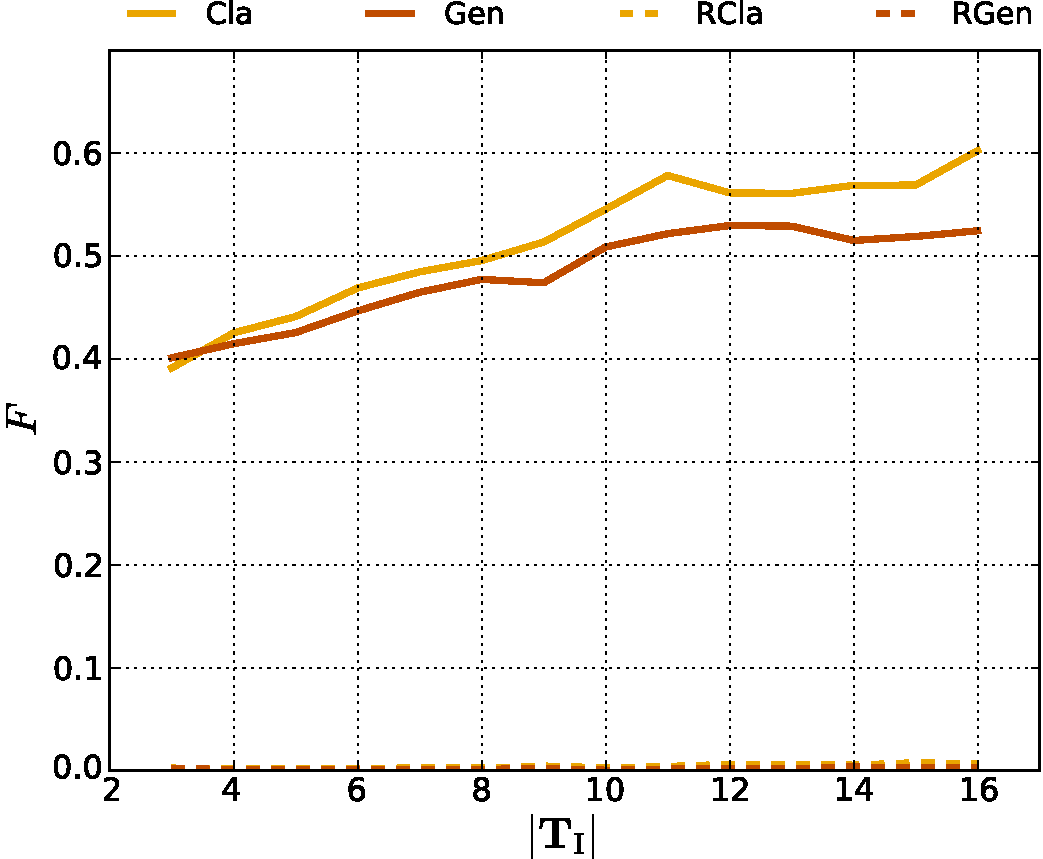
\includegraphics[width=\figSizeMid] {ch04_class/pics/fig_pb_evaluation_f_vs_input_tags.pdf}
      }
      \subbottom[]{
	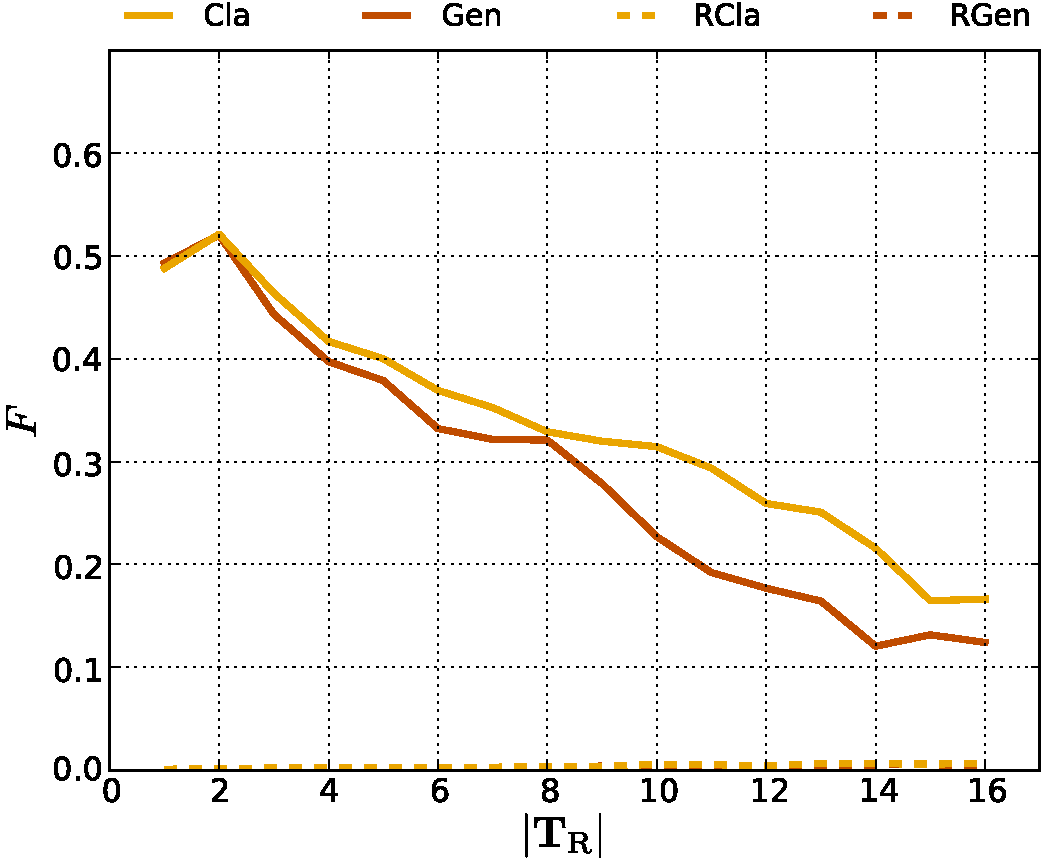
\includegraphics[width=\figSizeMid] {ch04_class/pics/fig_pb_evaluation_f_vs_added_tags.pdf}
      }
     \caption[Average f-measure as a function of the number of input tags and the number of recommended tags]{Average f-measure $\fmeasure$ as a function of the number of input tags $|\inputTags|$ (a) and the number of recommended tags $|\recommendedTags|$ (b).}
  \label{class:fig:f_measure_pb_evaluation}
\end{figure}


\section{Conclusion and discussion}
\label{class:sec:discussion}

In this chapter we have described an extension of the best performing tag recommendation method described in Chapter~\ref{sec:general}, and thoroughly evaluated it.
The method we described here extends the former in two main aspects: it automatically determines to which class a sound belongs, and it produces specific recommendations for different audio classes. 
As both tag recommendation methods (\textsc{Gen} and \textsc{Cla}) are folksonomy-based, they are easily generalisable to other multimedia domains. However, the \textsc{Cla} method requires the definition of a number of classes of resources in the particular domain, and the construction of a ground truth to train the classifier needed to perform recommendations. 

%The main bottleneck in terms of scalability lies in the computation of the tag-tag similarity matrices that inform the candidate selection step. However, these matrices can be computed offline, and their size can be easily reduced by raising the threshold $\tagFrequencyThreshold$ during the construction of the association matrix. This will discard those tags whose frequency of occurrence is below that threshold (Sec.~\ref{class:sec:Gen}). That means that our recommendation methods can scale well to even bigger amounts of data, as the number of tags above the threshold $\tagFrequencyThreshold$ will grow much more slowly than the number of resources.

%A limitation of the proposed recommendation methods is that they can suffer the \emph{cold-start} problem if deployed to collaborative tagging systems which have not enough data to derive reliable tag-tag similarity matrices. 
%Although our recommendation methods have not been designed for collaborative tagging systems with scarce data, it would be interesting to evaluate how fast the methods could acquire enough data from user annotations in order to provide meaningful recommendations. 
%In other words, it would be interesting to investigate how big the folksonomy of a collaborative tagging system should be to enable our tag recommendation methods to provide meaningful recommendations. 
%We hypothesise that, on a first step of the implementation of the system, tag-tag similarity matrices would need to be recomputed very often as relatively small changes in the folksonomy could have a big impact on the resulting similarity matrix. In that case, the system would quickly learn from user tagging behaviour and recommendations would quickly start to become more diverse. Besides the similarity matrices, the \textsc{Cla} method also needs annotation data to train the classifier. However, a collaborative tagging system could start using the \textsc{Gen} method until enough data would be collected to build the ground truth and train the classifier.

We performed a user-based evaluation through an online experiment. In it, participants had to annotate several sounds with the help of the different tag recommendation strategies. We logged the activity of the participants and analysed these logs with the goal of comparing the considered methods and, in addition, getting more insight into the positive and negative aspects of tag recommendation systems in general. To the best of our knowledge, this is one of the very few user-based evaluations carried out for a tag recommendation task. Finally, as a further contribution, we complement the user-based evaluation with a prediction-based evaluation, following a well-established methodology.

In general, we have seen that class-based recommendation reports statistically significantly better scores than general recommendation, both in the user-based and prediction-based evaluations. The difference in scoring is, in absolute terms, more prominent for the user-based evaluation. Moreover, it further improves when considering only expert users. This suggests that the class-based method does indeed bring some improvements in the recommendations compared to the general method, and that these improvements are more noticeable to expert users.

Among all annotations that participants performed during the online experiment, approximately one third of them correspond to tags recommended by the system (for both \textsc{Gen} and \textsc{Cla} methods). That by itself brings evidence with regard to the general utility of tag recommendation systems. However, the found results also indicate that tag suggestions referring to generic concepts or sound classes tend to be more useful than recommendations of very concrete tags describing specific sound characteristics. Participants found tag suggestions more useful for sounds under \textsc{Soundscape} and \textsc{Voice} categories. We hypothesise that this happens because these categories are more suited to the use of generic tags. \textsc{Music} and \textsc{Sample} audio classes require of annotations describing very specific musical concepts such as pitch, tonality or beats per minute. Participants had difficulties in annotating such concepts, as they are problematic to annotate without having a certain knowledge of the recording context (i.e.,~without being the author of the sound) and because tag recommenders tend to produce less meaningful suggestions in these cases. %All these often overlooked qualitative evaluation aspects also represent a valuable contribution of the present article.

Summarising, here we continued with the research described in the previous chapter by proposing an extended tag recommendation method that incorporates basic knowledge of the audio domain, and by comparing, with an online experiment, the extended method with the best scoring method of the previous tag recommendation scheme.
In the next chapter (Chapter~\ref{sec:impact}), we further investigate on tag recommendation by analysing the impact of the class-based method in a large-scale experiment on the real-world tagging system of Freesound.


% I REMOVED THIS BIT AS WE ALREADY COMNMENT ON THAT AT THE CONCLUSION OF THE NEXT CHAPTER
%Leaving aside the potential impact of tag recommendation in a real-world tagging system, we believe that in order to build better tag recommendation systems, those must be more aware of the particular contexts of the resources being described and must extensively exploit all available knowledge. To generate tag suggestions describing more concrete aspects of sound characteristics we need systems that know about the specifics of the audio domain, such as which are the most relevant properties of sounds for different audio categories, and how to automatically estimate some of these properties. In Chapter~\ref{sec:ontology}, we explore this perspective by proposing an extension of the tag recommendation method described here which takes advantage of a domain-specific ontology to drive the recommendation process.


%For that reason, we believe that future tag recommenders should take advantage of knowledge representation mechanisms such as ontologies to be able to include tags describing the audio domain in some structured representation, and to be able to produce informed recommendations based on reasoning and users' input. Such a system should contribute in greatly improving online resource descriptions and thus facilitating and providing new opportunities for content reuse.

% We have not investigated the use of more precise categories as our current goal is the classification of audio sounds in Freesound in broad categories that allow further tailored treatment, and not the classification of these audio sounds into a more specific taxonomy that could be used as an interface for browsing Freesound content. 

% We have also defined such categories so that they can, in a near future, allow us to apply meaningful different treatments tailored to different types of audio sounds
\cleartorecto%!TEX root = ../thesis_a4.tex

\chapter[Impact of a tag recommendation system][Impact of a tag rec. system]{Impact of a tag recommendation system}
\label{sec:impact}

\section{Introduction}
\label{impact:sec:introduction}


%Online sharing platforms make extensive use of semantically-meaningful textual labels, called tags, to describe and annotate its contents. The use of these tags provides a means for searching, browsing and organising the resources of the platform. Systems that provide the functionality for making these annotations are normally referred to as collaborative tagging systems. In collaborative tagging systems, users of the online platform have the responsibility of annotating the content. Every relation between a tag and a content resource performed by a user of the system can be identified as a tag application~\cite{Sen}, and we refer to the set of all distinct tags that are assigned to a particular resource as a \textit{tagline}. The aggregate of all tag applications, which relate tags, resources and users of an online sharing platform, is normally known as the folksonomy~\cite{Wal2007Folksonomy}.

%In general, tags introduced using collaborative tagging systems are not restricted in its form, and users can freely create new tags at any time~\cite{marlow2006,Sen,Wagner2014}. This provides a great flexibility to collaborative tagging systems as opposed to other systems that make use of pre-defined vocabularies and that do not allow users to annotate content using non-existing terms in these vocabularies~\cite{Robu2009,Wagner2014}. Using such non-restricted vocabularies, users introduce new tags when the annotation of a particular resource requires it. Hence, they easily adapt to the evolution of the platform's content. Furthermore, it has been suggested that users feel more comfortable during the annotation process when they are not restricted to the use of a pre-defined vocabulary~\cite{Robu2009}. 

%Collaborative tagging systems suffer from a number of well-known problems including tag scarcity, the use of different tags to refer to a single concept (synonymy), the ambiguity in the meaning of certain tags (polysemy), typographical errors, the use of user-specific naming conventions, or the use of different languages~\cite{halpin2006}. It is often discussed whether the folksonomy of a collaborative tagging system, after a certain time of being in use, reaches a point of implicit consensus where the vocabulary converges to a certain set of tags and tagging conventions that are widely adopted by all users of the system~\cite{halpin2006,Sen,Sood2007,Robu2009,Wagner2014}. Such a consensus implies more coherent resource annotations and better opportunities for searching, browsing and content organisation~\cite{Spiteri2006}. Additionally, it leverages the value of the folksonomy as a source of knowledge mining~\cite{Wagner2014}. Some studies have analysed this aspect, and the emergence of consensus has been highlighted in several occasions~\cite{Robu2009,Wagner2014}. 

%According to these studies, the emergence of consensus depends on several factors, one of them being the way in which users are exposed to the annotations performed by other users. In general, the more users are exposed to the tagging conventions of other users, the fastest should the consensus emerge. In order to try to overcome some of the issues of collaborative tagging systems, tag recommendation systems can be employed to suggest potentially relevant tags during the annotation process of a resource~\cite{jaske2007}. These systems are generally based on the analysis of the content of the resources being annotated, or in the folksonomy of a collaborative tagging system. Former systems normally use feature extraction techniques to analyse content resources, and further training of machine learning models that can predict tags based on the extracted features (e.g.,~\cite{Li2006,turnbull2008,Toderici2010}). Folksonomy-based systems normally take advantage of tag co-occurrence information in previously annotated resources in order to provide relevant tag recommendations for newly annotated resources (e.g.,~\cite{Sigurbjornsson2008,Garg2008,DeMeo2009,ivanov2010,Font2013}).

%It can be intuitively hypothesized that a tag recommendation system, independently of its nature, should have an impact on the folksonomy of a collaborative tagging system. In fact, this has been suggested by many authors. \cite{golder2006} hypothesize that a tag recommendation system should help consolidating the tag vocabulary across users. The same idea is suggesed by J\"{a}schke et~al.~\cite{jaske2007} and Marlow et~al.~\cite{marlow2006}. J\"{a}schke et~al.~\cite{jaske2007,Jaschke2012} also hypothesize that tag recommendation should simplify the process of finding good tags for the resources being described and thus increase the chances of getting resources annotated.
%Similarly, Sood et~al.~\cite{Sood2007} hypothesize that by using a tag recommendation system, users can see how other users tag resources and better choose when to reuse already existing tags or when to create new ones. Therefore, tag recommendation should help alleviate synonymy problems and help vocabulary convergence~\cite{Sood2007}. These authors also hypothesize that the use of a tag recommendation system fundamentally changes the tagging process from being a generation process, where users must create tags from scratch, to being a recognition process, where users have to recognise valid tags from a list of suggestions. Zangerle et~al.~\cite{Zangerle2011} perform a study on \emph{hashtag} recommendation for Twitter\footnote{http://www.twitter.com}, a microblogging site, and hypothesize that the use of hashtag recommendation should help homogenising hashtags. Finally, Wang et~al.~\cite{Wang2012} hypothesize that tag recommendation can improve both the quality of tags and the efficiency of the tagging process, by clarifying the semantics of tags and reducing the manual cost of tagging.

In the previous chapters we have described a number of tag recommendation methods and evaluated them from different perspectives. In this chapter, we perform a large-scale experiment in which we analyse the impact of a tag recommendation system in the real-world folksonomy of Freesound. More specifically, we introduce the best performing recommendation method described in Chapter~\ref{sec:general} (RankP@$\percentageOfPercentageStrategy$, with$\percentageOfPercentageStrategy=0.15$) to the tagging system of Freesound with the classification extension described in Chapter~\ref{sec:class}, and analyse its impact on the site.

As we have seen in the literature review, many authors have hypothesised about the potential impact of tag recommendation in the folksonomies of online sharing sites (Sec.~\ref{sec:soa:impact_tag_recommendation}). Taking this into consideration, we can summarise the expected impact into the following three hypotheses:
\begin{enumerate}
\item \textit{Vocabulary convergence.} A tag recommendation system should contribute to the convergence and consolidation of a shared vocabulary across the users of a tagging system~\citep{golder2006,marlow2006,jaske2007,Sood2007,Zangerle2011}.
\item \textit{Quality of annotations.} A tag recommendation system should improve the quality of resource annotations in an online sharing platform~\citep{Naaman2008,Jaschke2012,Wang2012}.
\item \textit{Cost of the annotation process.} A tag recommendation system should reduce the cost of tagging, changing from a tag generation process to a tag recognition process~\citep{Sood2007,jaske2007,Wang2012}.
\end{enumerate}

Although there seems to be a consensus on the hypotheses, we are not aware of any study performing a deep analysis of the impact of a tag recommendation system into a real-world and large-scale folksonomy. Furthermore, even though several studies have focused on analysing aspects such as tagging behaviour or vocabulary convergence in tagging systems (Chapter~\ref{sec:SOA}), there is not a clearly defined set of evaluation metrics or methodology to carry out these analyses~\citep{farooq2007}.

In this chapter, we define a series of metrics to illustrate each of the three summarised hypotheses. Then, we compute the defined metrics for an extensive period of time comprising 2.5 years of Freesound analysis data, including three months after the introduction of tag recommendation. We put a special emphasis on analysing the changes observed before and after the introduction of tag recommendation. Our results give, for the first time, empirical and quantitative evidence of the validity of some of the previous hypotheses.
Specifically, our results show that tag recommendation effectively contributes to vocabulary convergence, partially contributes to an improvement of the annotation quality, but does not seem to significantly reduce the cost of the annotation process. 
%In closing, some suggestions are made regarding how could tag recommendation systems be improved to further increase the impact on some of the analysed aspects such as the quality of the annotations. 
Notice that both the definition of the metrics and the analysis of its results are relevant contributions of the present chapter.

The rest of this chapter is organised as follows. 
In Sec.~\ref{impact:sec:methodology}, we briefly summarise the components of the tag recommendation system that we implemented, and describe the evaluation metrics and analysis methodology. The results for all evaluated metrics, along with discussions about their implications, are reported in Sec.~\ref{impact:sec:results}. 
%In Sec.~\ref{impact:sec:discussion} we summarise our findings and discuss about the limitations of our analysis.
We end in Sec.~\ref{impact:sec:conclusion} with a discussion about our findings and future directions.


%%%%%%%%%%%%%%%%%%%%%%%%%%%%%%%%%%%%%%%%%%%%%%%%%%%%%%%%%%%%%%%%%%%%%%%%%%%%%%%%%%%%%%%%%%%%%%%%%%%%%%%%%%%%%
\section{Methods}
\label{impact:sec:methodology}


%%%%%%%%%%%%
\subsection{Tag recommendation algorithm}
\label{impact:sec:tag_recommendation_system}

As mentioned, the recommendation method implemented in the tagging system of Freesound corresponds to the class-based approach described in Chapter~\ref{sec:class}.
In summary, it is composed of the three main steps described in Chapter~\ref{sec:general} plus the class detection step added in Chapter~\ref{sec:class} (see Fig.~\ref{impact:fig:diagram}).
Given a set of input tags $\inputTags$, the recommendation method is able to generate several lists of candidate tags $\candidateTagsPerInputTag$ taking advantage of a tag-tag similarity matrix $\similarityMatrixOfClassH$ which is, in turn, derived from the analysis of a folksonomy $\folksonomy$. 
A particular similarity matrix $\similarityMatrixOfClassH$ is chosen after a class detection step in which the system predicts the audio class $\audioClass$ that better fits $\inputTags$.
%Several similarity matrices $\similarityMatrixOfClassH$ are precomputed which are tailored to particular audio classes $\audioClass$. 
%In the class detection step, the recommendation method can predict which audio class $\audioClass$ better fits $\inputTags$, and then use the corresponding similarity matrix. 
The different sets of candidates $\candidateTagsPerInputTag$ are then aggregated into a single set of tags with scores $\aggregatedCandidateTags$.
Finally, a simple heuristic is applied to decide which of the tags in $\aggregatedCandidateTags$ are relevant enough to form the set of recommended tags $\recommendedTags$ outputted by the recommendation method.

\begin{figure}
\centerline{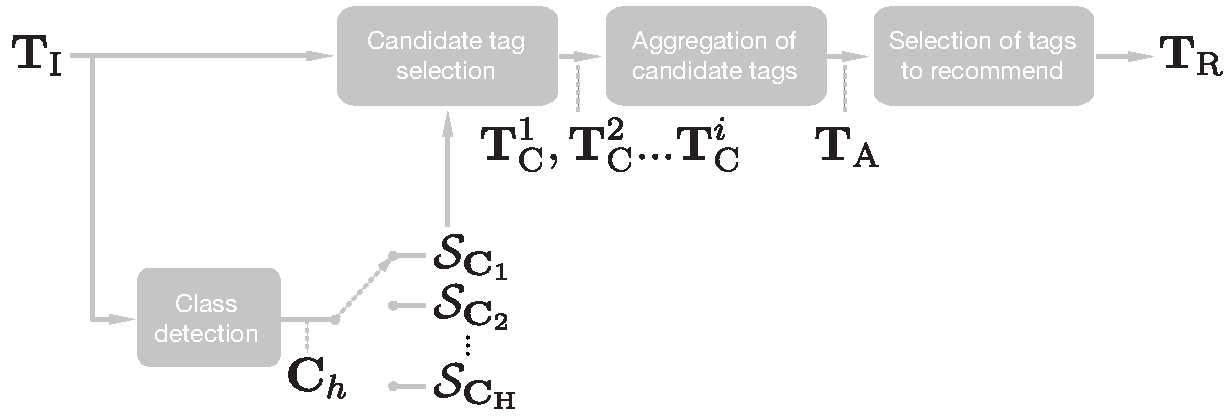
\includegraphics[width=\figSizeMidLarge]{ch05_impact/pics/fig01_diagram}}
\caption[Block diagram of the tag recommendation method implemented in Freesound]{Block diagram of the tag recommendation method implemented in the tagging system of Freesound.} 
\label{impact:fig:diagram}
\end{figure}

%\begin{enumerate}
%\item Class detection: The first step consists in the classification of the input tags $\inputTags$ into a set of $\nAudioClasses$ predefined audio classes. We defined $\nAudioClasses=5$ audio classes (\emph{SoundFX}, \emph{Soundscape}, \emph{Sample}, \emph{Music} and \emph{Speech}), and built a ground truth by manually annotating 1,200 Freesound sounds per class~\cite{Font2013a}. Using this ground truth, we trained a multivariate Bernoulli naive Bayes classifier, feeding it with the taglines of the sounds. Then, given a set of input tags $\inputTags$, the classifier can predict which category $\audioClass$ better fits the input.  Accuracies range between 75 and 95\%, depending on the length of $\inputTags$.

%\item Candidate tag selection: Given the set of input tags $\inputTags$, this step selects a pool of candidate tags $\candidateTagsPerInputTag$ for each input tag $\inputTag$. We do so by choosing the top 100 most similar tags according to a tag-tag similarity matrix $\similarityMatrix_{\audioClass}$, which depends on the predicted class $\audioClass$ of the previous step. Matrices $\similarityMatrix_{\audioClass}$ are computed offline and considering a model of the folksonomy of Freesound $\folksonomy$, which is represented as a tripartite hypergraph $\graph(\folksonomy)=\left\langle \vertices,\edges \right\rangle$~\cite{Mika2007a,Font2013}. In this model, vertices are given by three finite sets of objects, $\vertices=\users\cup \tags\cup \resources$ (users, tags and resources, respectively), and each edge $\edges=\{\{\user,\tagb,\resource\}| (\user,\tagb,\resource)$ $\in \folksonomy\}$ represents a tag application, embedding a relation between a tag $\tagb$, a resource $\resource$ (a sound), and the user $\user$ that performed that tag application. Given this model, we derive a sparse association matrix $\associationMatrix = \left\{ \associationMatrix_{i,j} \right\}$, $i=1,\dots |\resources|$, $j=1,\dots |\tags|$, which represents the associations between the $|\resources|$ sounds and the $|\tags|$ distinct tags available in Freesound ($\associationMatrixElement_{i,j} = 1$ if sound $\resource_i$ is labeled with tag $\tagb_j$, and $\associationMatrixElement_{i,j} = 0$ otherwise). 
%We use the same classifier used in the class detection step to predict the class of all sounds in the association matrix given their tag associations. Then, given $\associationMatrix$ and the list of sounds we predicted for every class $\audioClass$, we can compute the different tag-tag similarity matrices by filtering out all columns from $\associationMatrix$ corresponding to sounds which do not belong to a particular class and then performing a matrix multiplication so that $\similarityMatrix_{\audioClass} = \associationMatrixMultiplication'$, where $'$ indicates matrix transposition. Applying a simple normalisation to the elements of $\similarityMatrix_{\audioClass}$, we obtain a matrix whose elements $\left\{ \similarityMatrix_{\tagb_i,\tagb_j} \right\}$ correspond to the cosine similarity between tags $\tagb_i$ and $\tagb_j$ on the context of a particular audio class $\audioClass$~\cite{Font2013,Font2014}.

%\item Aggregation of candidate tags: Given the sets $\candidateTagsPerInputTag$ from the first step, candidates are assigned a score $\scoreCandidateTag$ and aggregated into a single list of tags with scores $\aggregatedCandidateTags$. Such score is determined by the candidate similarity-based ranking so that $\scoreCandidateTag=1$ for the most dissimilar candidate to a given input tag and $\scoreCandidateTag=N$ for the most similar one. The scores of tags that are present in different sets of candidates $\candidateTagsPerInputTag$ are added when aggregated to the final set $\aggregatedCandidateTags$~\cite{Font2013}.

%\item Selection of tags to recommend: Considering the scores in $\aggregatedCandidateTags$, this step determines a threshold $\scoreThreshold$ to select the tags that are finally recommended. The threshold $\scoreThreshold$ is set to be the 85\% of the maximum score in $\aggregatedCandidateTags$. Tags in $\aggregatedCandidateTags$ are sorted by their score and those that satisfy $\scoreCandidateTag \geq \scoreThreshold$ are outputted as $\recommendedTags$, the final set of recommended tags~\cite{Font2013}.
%\end{enumerate}

%%%%%%%%%%%%
\subsection{Tag recommendation interface}
\label{impact:sec:tag_rec_interface}

Fig.~\ref{impact:fig:screenshot_system} shows a screenshot of the interface for the tag recommendation system implemented in Freesound. In it, we can see the set of input tags $\inputTags=$\{\texttt{river}, \texttt{water}\} and the set of recommended tags $\recommendedTags=$\{\texttt{stream}, \texttt{creek}, \texttt{brook}, \texttt{flow}, \texttt{liquid}, \texttt{waterfall}, \texttt{trickle}\}. The list of suggested tags appears at the bottom of the text area that users use to type their tags, and it is automatically refreshed each time that users type a new tag (i.e.,~every time that there is a change in $\inputTags$). 
This means that during the annotation process of a particular sound, several lists of recommended tags are presented to the user. To introduce tags from the list of recommendations, users can either click on the elements of the list or type them manually (as they would do to introduce other tags that are not in the list). When manually typing tags, no autocomplete functionality is provided. 

\begin{figure}
\centerline{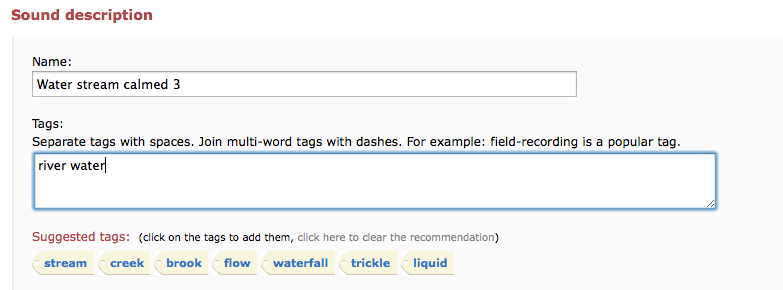
\includegraphics[width=1.0\columnwidth]{ch05_impact/pics/fig02_screenshot_system}}
\caption[Screenshot of the tagging interface of Freesound]{Screenshot of the tagging interface of Freesound after introducing the tag recommendation method. The previous interface (before the introduction of the tag recommendation), was exactly the same without the list of tag suggestions at the bottom.} 
\label{impact:fig:screenshot_system}
\end{figure}


%%%%%%%%%%%%
\subsection{Analysis metrics}
\label{impact:sec:definition_of_metrics}

To assess the impact that the tag recommendation system has on the folksonomy of Freesound, we define a series of metrics which are meant to illustrate the three hypotheses summarised in the introductory section of this chapter (Sec.~\ref{impact:sec:introduction}). 
Rather than the observation of a single metric being affected after the introduction of the tag recommendation system, we believe the relevance of the analysis particularly remains on the observation of changes simultaneously happening in several metrics. Hence, we illustrate each hypothesis with more than one metric.
Table~\ref{tab:hypothesis_metrics} shows a list of the defined metrics, along with the changes we expect to observe when comparing data before and after the introduction of the tag recommendation system. Formal metric definitions subsequently follow, grouped by hypothesis. 


\begin{table}
\ra{1.2}
\begin{center}
\footnotesize
	\begin{tabular}{p{3.7cm}P{4.8cm}P{3cm}}
	\toprule
	\textbf{Hypothesis} & \textbf{Metric} & \textbf{Expectation} \\
	\midrule
	\multirow{4}{3.7cm}{Vocabulary convergence}
	       & Percentage of new tags & Decrease \\
	 
	       & Average user vocabulary size & Increase \\ 
       	       & User vocabulary sharing & Increase \\ 
	       & Sound vocabulary sharing & Increase \\ 
	\\
	\multirow{5}{3.7cm}{Quality of annotations}
	       & Average tagline length & Increase  \\
	       & Percentage of misspelled tag applications & \multirow{2}{3cm}{Decrease}  \\ 
	       & Tag frequency distribution & Even (see caption)  \\ 
	       & Subjective annotation quality & Increase \\
	\\
	\multirow{3}{3.7cm}{Cost of the annotation process}
	       & Average tag application time & Decrease  \\
    	   & Average number of correctly predicted tags & \multirow{2}{3cm}{Similar to Sec.~\ref{class:sec:accepted_tags_results}}  \\
    \bottomrule
	\end{tabular}
\end{center}
\caption[Proposed metrics and expected observations]{Proposed metrics and expected observations to evaluate the hypotheses. In the case the tag frequency distribution, we expect a more even distribution across the frequency range after the introduction of tag recommendation.}
\label{tab:hypothesis_metrics}
\end{table}


\subsubsection{Vocabulary convergence}

\begin{itemize}
	\item \textit{Percentage of new tags}: This metric represents the percentage of the tag applications that were performed during a given day of our analysis period, and that had never been used before in the folksonomy (i.e.,~tag applications that introduce previously nonexistent tags in the folksonomy). Thus, this metric is computed on a daily basis (see Sec.~\ref{impact:sec:analysis_methodology}). Considering the folksonomy model defined in Sec.~\ref{sec:general:step1}, the percentage of new tags can be defined as
\begin{equation} \metricVocabularyConvergence(n) = 100 \cdot \frac{|\setOfNewTagsInDay|}{|\setOfTagApplicationsInADay|}, \label{impact:eq:percentage_of_new_tags} \end{equation}
where $\setOfNewTagsInDay$ is the set of tags that appeared for the first time in the $n$-th day of our analysis data, and $\setOfTagApplicationsInADay$ is the set of all tag applications performed during that same day. Note that $\setOfNewTagsInDay$ can not contain duplicates (i.e.,~a particular tag can not be considered as being ``new'' more than once). High values of $\metricVocabularyConvergence$ indicate that many new tags are being created and that, therefore, the vocabulary is not converging to a finite set of terms. Our expectation is that $\metricVocabularyConvergence$ will decrease after the introduction of tag recommendation, as users will tend to reuse tags from the list of suggestions rather than creating new ones.
		
	\item \textit{Average user vocabulary size}: This metric is also computed on a daily basis, and we define it as the total number of tag applications involving distinct tags that a user performed during a given day (i.e.,~the number of unique tags that a user assigned during a given day). Considering the folksonomy model defined in Sec.~\ref{sec:general:step1}, the average vocabulary size can thus be expressed as
\begin{equation} \metricAverageVocabularySize({n}) =  \frac{1}{|\setOfUsersPerformingTagApplicationInDay|}\sum\limits_{\user\in \setOfUsersPerformingTagApplicationInDay}{|\setOfTapplicationsDistinctTagsPerUserAndDay|}, \label{impact:eq:user_vocabulary_size} \end{equation}
where $\setOfTapplicationsDistinctTagsPerUserAndDay$ is the set of tag applications involving distinct tags that user $\user$ has performed during the $n$-th day of our analysis data, and $\setOfUsersPerformingTagApplicationInDay$ is the set of users that performed at least one tag application during that same day. High values of $\metricAverageVocabularySize$ indicate that users employ a wide variety of tags for annotating their sounds, whereas low values indicate that users tend to employ a restricted vocabulary of tags. We believe that when using the tag recommendation system users will be exposed to a wider variety of tags than the ones that they would have initially thought of. Hence, we expect to observe an $\metricAverageVocabularySize$ increase after the introduction of tag recommendation.

	\item \textit{User vocabulary sharing}: This metric quantifies to which extent users employ tags that have also been employed by other users. To analyse this aspect, we build a weighted network $\usersNetwork$ where nodes represent users and edges represent the amount of tags shared between two users. Edge weights $\edgeWeight$ between nodes $i$ and $j$ of $\usersNetwork$ are normalised using standard Jaccard similarity. Thus, given an arbitrary period of time $k$ for which a network $\usersNetwork_k$ can be constructed, the weight between two nodes can be computed as
\begin{equation}\edgeWeight_{ij} = \frac{ \left\vert \setOfDistincTagsPerUserAndPeriod \cap \setOfDistincTagsPerUserAndPeriodJ \right\vert }{ \left\vert \setOfDistincTagsPerUserAndPeriod \cup \setOfDistincTagsPerUserAndPeriodJ \right\vert }, \label{impact:eq:weight_vocabulary_sharing} \end{equation}
where $\setOfDistincTagsPerUserAndPeriod$ is the set of distinct tags that the user corresponding to the $i$-th node has annotated during the time period comprised in $k$ (similarly for $\setOfDistincTagsPerUserAndPeriodJ$ and node $j$). 
In such a network, two users will be strongly connected if they use the same tags when annotating their sounds. Notice that, according to the definition above, every node in $\usersNetwork_k$ has a self-loop, i.e.,~for $i=j$ we have $\edgeWeight_{i,j}=1$. Having defined $\usersNetwork_k$, node strength~\citep{Barrat2004} acts as a basic indicator of the level of vocabulary sharing across users. The more strength the nodes have, the more tags users are sharing. 
Let $\nNodes$ be the total number of nodes in $\usersNetwork_k$, and $\nodeStrength_i$ be the node strength for the $i$-th node of $\usersNetwork_k$ such that
\begin{equation} \nodeStrength_i = \sum\limits_{j=1}^{L}{w_{ij}}. \end{equation}
We define user vocabulary sharing $\metricUserVocabularySharing$ as the average node strength over the network so that
\begin{equation} \metricUserVocabularySharing(\usersNetwork_k) = \frac{1}{\nNodes}\sum\limits_{i=1}^{\nNodes}{\nodeStrength_i}. \label{impact:eq:user_vocabulary_sharing} \end{equation}

In our analysis, we build two networks $\usersNetwork_k$ as defined above, one considering all the data after the introduction of tag recommendation and the other considering data from a reference time window before the introduction of tag recommendation (see below). We compare these two networks by computing the difference between user vocabulary sharing (average node strength) in both networks. We asses the statistical significance of that comparison by taking the series of node strengths of both networks (i.e.,~without computing the average) and using the Kolmogorov-Smirnov two-sample test~\citep{Corder2009} for evaluating the null hypothesis that both node strength samples belong to the same distribution (we use a significance level of 0.01). After the introduction of tag recommendation, we expect to observe an increase in $\metricUserVocabularySharing$, as users will be highly exposed to the influence of tags used by other users, and therefore more links will be created in $\usersNetwork$.

	\item \textit{Sound vocabulary sharing}: Similar to the previous metric, we can also study the vocabulary sharing across sounds instead of users. In this way, sound vocabulary sharing represents the tags that sounds have in common. To analyse sound vocabulary sharing, we build a weighted network $\soundsNetwork$ where nodes represent sounds and edges represent the number of tags that are common in the two sounds linked by the edge. As in $\usersNetwork$, edge weights are normalised using the Jaccard similarity. Hence, the weight $\edgeWeight$ between nodes $i$ and $j$ of a network $\soundsNetwork_k$ computed with data from a time period $k$, can be defined as
\begin{equation} \edgeWeight_{ij} = \frac{ \left\vert \tagsAssignedToSoundI \cap \tagsAssignedToSoundJ \right\vert }{ \left\vert \tagsAssignedToSoundI \cup \tagsAssignedToSoundJ \right\vert }, \label{impact:eq:weight_sound_sharing} \end{equation}
where $\tagsAssignedToSoundI$ is the set of tags assigned to the sound represented by the $i$-th node (similarly for $\tagsAssignedToSoundJ$ and node $j$). Notice that, in this case, the definition of $\edgeWeight_{ij}$ does not include the time period $k$ in any of its terms. This is because all tag applications for a given sound are done at once. Therefore, if the sound was uploaded in the time period $k$ (and thus is represented by a node in the network $\soundsNetwork_k$), all its tag applications will have also been performed during that time period $k$. In $\soundsNetwork_k$, two sounds will be strongly connected if they are annotated with the same tags, and we consider node strength as a basic indicator of the vocabulary sharing across sounds. 
Thus, we can define sound vocabulary sharing $\metricSoundVocabularySharing$ for a network $\soundsNetwork_k$ as the average node strength over that network, and compute it in the same way as described for user vocabulary sharing.

%Therefore, we can define sound vocabulary sharing as the average node strength over a network $\soundsNetwork_k$ with $\nNodes$ nodes, so that
%\begin{equation} \metricSoundVocabularySharing(\soundsNetwork_k) = \frac{1}{\nNodes}\sum\limits_{i=1}^{\nNodes}{\sum\limits_{j=1}^{\nNodes}{\edgeWeight_{ij}}}. \label{impact:eq:sound_vocabulary_sharing} \end{equation}

For analysis purposes, we again build two networks with data before and after the introduction of tag recommendation. The two networks are compared in terms of their node strength following the same process described above for analysing user vocabulary sharing. After the introduction of tag recommendation, we expect to observe an increase in $\metricSoundVocabularySharing$, as users will be highly exposed to the influence of tags used by other users. Therefore, sound annotations will include these tags and more links will be created in the network $\soundsNetwork$.

\end{itemize}


\subsubsection{Quality of annotations}
\label{impact:sec:methods_quality_of_annotations}

\begin{itemize}

	\item \textit{Average tagline length}: This metric is computed on a daily basis, and we define it as the average number of tags assigned to sounds uploaded during a given day of our analysis period. Considering the folksonomy model defined in Sec.~\ref{sec:general:step1}, the average tagline length can be expressed as
\begin{equation} \metricAverageTaglineLength(n) =  \frac{1}{|\soundsUploadedInDay|}\sum\limits_{\resource\in \soundsUploadedInDay}{|\tagsOfSoundR|}, \label{impact:eq:average_tagline_length} \end{equation}
where $\tagsOfSoundR$ is the set of tags assigned to a resource $\resource$ and $\soundsUploadedInDay$ is the set of sounds uploaded and annotated during the $n$-th day of our analysis. High values of $\metricAverageTaglineLength$ indicate that sounds are being annotated with many tags, with potentially more comprehensive descriptions. Our expectation for this metric is to observe an increase after the introduction of tag recommendation, as the provided list of recommendations will help users to add more tags during the annotation process. In fact, even if recommendations are not appropriate, they may serve as a guide for users, and convey which kinds of information should be annotated about the sounds being described. For instance, the recommendation system could suggest a tag like \texttt{120bpm} to a sound sample corresponding to a music loop of different tempo. However, this tag might suggest to the user that she could describe tempo information, and help in this way to generate a longer tagline. %~\cite{Font2014}.
Hence, we expect $\metricAverageTaglineLength$ to be increased after the introduction of tag recommendation.


	\item \textit{Percentage of misspelled tag applications}: This metric represents the percentage of tag applications that contain tags with misspellings or typographical errors and that were performed during a given day of our analysis period. Considering the folksonomy model defined in Sec.~\ref{sec:general:step1}, the percentage of misspelled tag applications can be defined as
\begin{equation} \metricMispellings(n) = 100 \cdot \frac{|\setOfTagApplicationsInADayWithMisspellings|}{|\setOfTagApplicationsInADay|}, \end{equation}
where $\setOfTagApplicationsInADay$ is the set of all tag applications performed during the $n$-th day of our analysis data, and $\setOfTagApplicationsInADayWithMisspellings$ is the set of tag applications performed during that same day which involve misspelled tags.
In order to estimate $\setOfTagApplicationsInADayWithMisspellings$, we use a straightforward approach in which we check, for each individual tag, whether if it exists or not in an English dictionary. For that purpose we use the open-source Enchant spellchecking library, with British English and American English dictionaries\footnote{\url{http://www.abisource.com/projects/enchant/}.} \citep[similarly to][]{Guy2006}. 
We consider that the tags which do not appear in the English dictionary contain misspellings or typographical errors.
Using such a simple approach, tags consisting of proper nouns, compound words, or tags written in other languages, are most likely considered to be misspellings. However, we assume that the presence of these kind of tags is not affected by the introduction of the tag recommendation system, and thus our defined metric is meaningful enough for comparison purposes.
High values of $\metricMispellings$ indicate that many of the tags assigned to sounds contain misspellings. 
Our expectation is that $\metricMispellings$ should decrease after the introduction of tag recommendation, as users will manually type fewer tags and choose them from the list of recommendations instead.


	\item \textit{Tag frequency distribution}: One useful indicator of the impact of the tag recommendation system is the observation of changes in the frequency distribution of existing tags. 
Intuitively, tags that are very popular (i.e.,~that have a high frequency) tend to correspond to broader semantic concepts, while less popular tags usually correspond to narrower ones. Looking at the tag frequency distribution we can thus have an idea of users' tagging behaviour and observe if it is influenced by the tag recommendation system.
To do that, we compute the frequency of tags over a period of time $k$ such that the frequency $\tagFrequency$ of a tag $\tagb$ is expressed as
\begin{equation} \tagFrequency(\tagb,k) = |\tagApplicatonsPerTagT|, \label{impact:eq:tag_frequency} \end{equation}
where $\tagApplicatonsPerTagT$ is the set of all tag applications involving tag $\tagb$ during the time period $k$. We consider two time periods, one with data before the introduction of tag recommendation and the other with data after tag recommendation, and compute the complementary cumulative distribution of tag frequencies over the two periods. These kind of plots are common within the tagging literature~\citep{Bischoff2008,Robu2009}, and indicate the probability that the number of occurrences of a particular tag is above a certain level. By qualitatively comparing the resulting distribution over the two periods of time, we can have an idea of which frequency ranges are more affected by the tag recommendation system. We believe that the tag recommendation system will have a bigger impact on the tags with mid frequency of occurrence, in which the agreement in not as clear as in the tags with high frequencies. Therefore, our expectation for this metric is that we will observe a more even tag frequency distribution after the introduction of tag recommendation.

Additionally, we compare the distribution of tag frequencies before and after the introduction of tag recommendation in terms of their fit into a power law distribution. As mentioned, it has been suggested that folksonomies whose distribution of tag frequencies can be fitted by a power law exhibit mature vocabularies leading to better quality descriptions (Sec.~\ref{sec:soa:impact_tag_recommendation}). %~\citep{Mathes2004,Cattuto2006,halpin2006,Wagner2014}. 
Hence, we check if we observe any difference regarding this matter after the introduction of tag recommendation. %\ref{sec:soa:impact_tag_recommendation}
To check whether a distribution is well fitted by a power law we use the method proposed by~\cite{Clauset2007}\footnote{We use the open source implementation described in~\cite{Alstott2014}.}.
This analysis is also directly related with the hypothesis that tag recommendation should contribute to the convergence and consolidation of the vocabulary.

	\item \textit{Subjective annotation quality}: We are interested in analysing whether the tag recommendation system has an impact on the quality of sound annotations. To avoid having to define an objective metric for quality, we opt for measuring quality in relative terms, by comparing the subjective quality of a set of annotations before and after the introduction of tag recommendation. To do so, we set up a small online experiment where participants were presented with pairs of sounds from Freesound along with their taglines, and had to judge which sound was, in their opinion, better annotated. Every pair of sounds consisted of one sound uploaded after the introduction of tag recommendation and another sound uploaded before that. Sounds were labeled as ``Sound A'' and ``Sound B'', without providing any links to the original sounds in Freesound and without giving any hint of which sound was uploaded before and after the introduction of tag recommendation (Fig.~\ref{impact:fig:screenshot_experiment}). For every participant, sound pairs were presented in random order, and the assignment of each sound as being ``Sound A'' or ``Sound B'', was also randomised. For every pair of sounds, participants could either answer that ``Sound A'' was better annotated than ``Sound B'', that ``Sound B'' was better annotated than ``Sound A'', or indicate that they did not think that one sound was better annotated than the other (``No preference''). If participants wanted to give further explanations for their answers, they also had the option to introduce a textual comment for every comparison.
	
\begin{figure}
\centerline{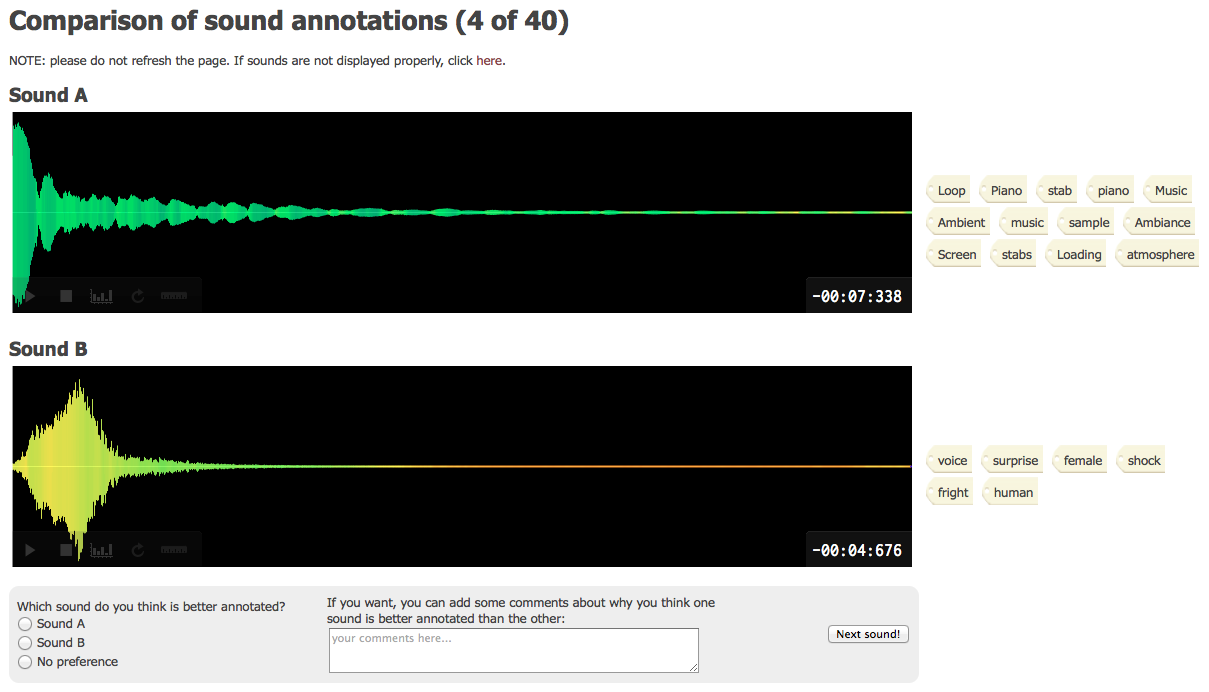
\includegraphics[width=1.00\columnwidth]{ch05_impact/pics/fig03_screenshot_experiment}}
\caption[Screenshot of the online experiment interface to judge the quality of annotations]{Screenshot of the online experiment interface to judge the quality of annotations.} 
\label{impact:fig:screenshot_experiment}
\end{figure}

Participants had to compare the annotation quality of a total of 40 sound pairs. To select the sounds for the experiment, we first randomly chose a set $\subjectiveEvaluationSetX$ of 40 sounds among those uploaded after the introduction of tag recommendation. The random selection was only constrained in such a way that all selected sounds had to be uploaded by different users. Then, we built another set $\subjectiveEvaluationSetY$ of 40 sounds uploaded before the introduction of tag recommendation. In order to build $\subjectiveEvaluationSetY$ and make it as similar as possible to $\subjectiveEvaluationSetX$ (i.e.,~containing similar kinds of recordings), we used the ``similarity search'' functionality of Freesound. For each sound $\subjectiveEvaluationSetX_i$, we retrieved a list of candidate similar sounds taking into account their acoustic properties represented by low-level audio descriptors\footnote{Low-level audio descriptors mainly include spectral features such as \emph{spectral centroid} and \emph{MFCC}. Note that the similarity search functionality does not take into account any metadata like tags or textual descriptions.}. Then, we pruned the lists of candidates by removing those sounds that were uploaded after the introduction of tag recommendation and by not allowing to have more than one sound uploaded by the same user. Finally, for each sound $\subjectiveEvaluationSetX_i$, we manually listened to the remaining candidates and selected the candidate that, in our opinion, was more acoustically similar to $\subjectiveEvaluationSetX_i$. %Set $\subjectiveEvaluationSetY$ was thus constructed with all  selected candidates. 
Having the sets $\subjectiveEvaluationSetX$ and $\subjectiveEvaluationSetY$, we formed the final pairs of sounds used in the experiment by iteratively selecting a random sound from each set until we got the 40 pairs determined. 

We asked the team of Freesound moderators\footnote{All sounds that are uploaded to Freesound are manually moderated by a small team of people (all of them long-term Freesound users) that ensure the appropriateness of the uploaded sounds. Hence, Freesound moderators are very familiarised with Freesound content and tagging particularities.} to participate in the experiment, and collected data from a total of seven participants (i.e.,~obtaining a total seven judgements for every sound pair). 	
Considering the collected data, we assign numerical values to the $i$-th quality judgement $\qualityJudgement_i$ performed by every participant such that
\begin{equation} \qualityJudgement_i = \begin{cases} 
	1 & \text{if } \subjectiveEvaluationSetX_i \text{ is better than } \subjectiveEvaluationSetY_i \\
	-1 & \text{if } \subjectiveEvaluationSetY_i \text{ is better than } \subjectiveEvaluationSetX_i \\
	0 & \text{if no preference.}
\end{cases} \label{impact:eq:quality_judgement_cases} \end{equation}
Then, qualitative annotation quality $\metricQualitativeAnnotationQuality$ is computed as the average over the union of all quality judgements $\qualityJudgement_i$ performed by all participants in the experiment. Let $\unionOfQualityJudgements$ be the union of all quality judgements $\qualityJudgement_i$. Then
\begin{equation} \metricQualitativeAnnotationQuality = \frac{1}{|\unionOfQualityJudgements|}\sum\limits_{j \in \unionOfQualityJudgements}{\unionOfQualityJudgements_j}. \label{impact:eq:quality_judgement_metric} \end{equation}
Note that a value of $\metricQualitativeAnnotationQuality$ close to $1$ indicates a preference for the annotations of sounds from $\subjectiveEvaluationSetX$ (i.e.,~sounds uploaded after the introduction of tag recommendation), while a value close to $-1$ indicates a preference for sounds from $\subjectiveEvaluationSetY$ (i.e.,~sounds uploaded before tag recommendation). A value close to $0$ indicates no preference. Our expectation for this metric is to obtain a positive value, indicating a tendency of considering sounds uploaded after tag recommendation as being better annotated than sounds uploaded before tag recommendation. This would suggest an increase in annotation quality.

\end{itemize}


\subsubsection{Cost of the annotation process}
\label{impact:sec:methods_cost_of_annotation}

\begin{itemize}

	\item \textit{Average tag application time}: An important indicator of how difficult it is for users to annotate sounds is the observation of the time they spend annotating them~\citep{Wang2012}. For that purpose, we define the average time per tag application as
\begin{equation} \metricAverageTagApplicationTime(\annotationSessions) =  \frac{1}{|\annotationSessions|}\sum\limits_{\annotationSession \in \annotationSessions}{\frac{\durationOfAnnotationSession}{|\tagApplicationsOfAnnotationSession|}}, \label{impact:eq:averae_tag_application_time} \end{equation}
where $\durationOfAnnotationSession$ is the duration of an annotation session $\annotationSession$ (in seconds), $\tagApplicationsOfAnnotationSession$ is the set of tag applications performed during an annotation session $\annotationSession$, and $\annotationSessions$ is a set of annotation sessions. Low $\metricAverageTagApplicationTime$ values indicate that users do not need much time to add a single tag, therefore it is presumably easy for them to describe sounds.

Unfortunately, Freesound did not log information about the duration of annotation sessions before the introduction of tag recommendation. Therefore, no data was available for most of the analysed time period. To overcome that issue, during a period of time that lasted two weeks between 24 March 2014 and 7 April 2014, we altered the tag recommendation system so that it only provided recommendations to half of the annotation sessions (but logged the annotation process in both cases). Therefore, our analysis of $\metricAverageTagApplicationTime$ is carried out with data gathered only during that extra analysis period. This data includes annotation sessions for 562 sounds, one half of them annotated using tag recommendation and the other half annotated without tag recommendation. Note that this new analysis period does not overlap with the period of the main analysis (see below).

We divide the annotation session data we gathered into two sets: one containing data from sessions were tag recommendations were not provided ($\annotationSessions^-$) and the other containing data from sessions with recommendations ($\annotationSessions^+$). Next, we compare the average $\metricAverageTagApplicationTime$ for both sets of annotation sessions and asses the statistical significance of the difference by performing the Mann-Whitney U test with a significance level of 0.01~\citep{Corder2009}. Our expectation for this metric is that sessions which provided tag recommendations will exhibit lower values of $\metricAverageTagApplicationTime$, as users will add some tags by clicking on the tag suggestions and this will make the annotation process faster.

	\item \textit{Average number of correctly predicted tags}: This is the main metric that we used in the user-based evaluation carried out in the previous chapter (Sec.~\ref{class:sec:evaluation}). It quantifies how many of the tags assigned to a sound during an annotation process were actually suggested by the recommendation system (thus correctly predicted). We follow the definition of Eq.~\ref{class:eq:n_accepted_tags}. However, here we define it on a daily basis such that
\begin{equation} 
%\metricPercentageOfCorrectlyPredictedTags(n) = \frac{1}{|\soundsUploadedInDay|}\sum\limits_{\resource\in \soundsUploadedInDay}{| \tagsOfSoundR \cap \setOfTagsSuggestedToSoundR |},
\nAcceptedTags(n) = \frac{1}{|\soundsUploadedInDay|} \sum\limits_{\resource\in \soundsUploadedInDay}{\left\vert \tagsOfSoundR \cap \left( \bigcup^{\numberOfTagRecommendationsInSession}_{\recommendationsInSessionIndex=1} \nthRecommendedTagsInSession \right) \right\vert}, 
\label{impact:eq:percentage_of_correctly_predicted_tags} \end{equation}
where $\tagsOfSoundR$ is the set of tags assigned to sound $\resource$, 
$\nthRecommendedTagsInSession$ is one of the sets of recommended tags that were presented to the user in the successive $\numberOfTagRecommendationsInSession$ recommendations during the tagging process of $\resource$, and $\soundsUploadedInDay$ is the set of sounds uploaded and annotated during the $n$-th day of our analysis data. Note that we can not compute $\metricPercentageOfCorrectlyPredictedTags$ for data before the introduction of tag recommendation. 

The average number of correctly predicted tags is an indicator of the usefulness of the tag recommendation system during the annotation process. High values of $\metricPercentageOfCorrectlyPredictedTags$ indicate that many of the tags that are recommended are actually used to annotate the sounds they are recommended for, and suggest that the annotation process is less costly as tags are taken from the list of suggestions. Our expectation for this metric is to obtain similar results as in the user-based evaluation of Chapter~\ref{sec:class} (Table ~\ref{tab:results_general_ub}). %In that case, the average number of correctly predicted tags was found to be 2.414 for the class-based tag recommendation method (Table ~\ref{tab:results_general_ub}).


\end{itemize}


%%%%%%%%%%%%
\subsection{Analysis methodology}
\label{impact:sec:analysis_methodology}

The impact of the tag recommendation system is analysed by looking at the evolution of the Freesound folksonomy (gathering data directly from the Freesound database) and the logs we create every time a user annotates a new sound. Our analysis comprises data between the 21 September 2011 and 28 February 2014. The tag recommendation system was introduced on 20 November 2013. The metrics defined in the previous section are either computed on a daily basis (using data from a particular day of our analysis), or over bigger periods of time (using data data gathered from several days of our analysis). To represent daily time periods, let $\mathbf{\daysVector}$ be a vector of time periods where $\daysVector_{n}$ corresponds to the time period of the $n$-th day since the beginning of our analysis data. In that vector, $\daysVector_{0}$ corresponds to the time period of the first day in our analysis data (21 September 2011), and $\daysVector_{N}$ corresponds to the time period of the last day for which we have analysis data (28 February 2014). 

In addition to what precedes, to represent larger periods of time, we define a series of analysis windows which include data from several days of our analysis. On the one hand, let $\windowOfInterest$ be our analysis window of interest, which represents a time period including all the data after the introduction of tag recommendation (i.e.,~a total of 100 days from 20 November 2013 to 28 February 2014). On the other hand, let $\referenceWindowsVector$ be a vector of reference analysis windows where each element $\referenceWindowsVector_{m}$ corresponds to a time period of the same length as $\windowOfInterest$ (100 days), drawn from data before the introduction of tag recommendation. The window $\referenceWindowsVector_{0}$ corresponds to the last 100 days before the introduction of tag recommendation (from the 12 August 2013, to 19 November 2013), and the $m$-th analysis window corresponds to a time period shifted backwards in time $50m$ days. Figure~\ref{impact:fig:analysis_windows} shows a graphical representation of $\mathbf{\daysVector}$ and $\referenceWindowsVector$, and the analysis window of interest $\windowOfInterest$. Notice that $\windowOfInterest$, as well as each element of $\referenceWindowsVector$, includes a particular range of $\daysVector$ time periods (e.g.,~$\windowOfInterest$ corresponds to $\daysVector_{N-100:N}$).

\begin{figure}
\centerline{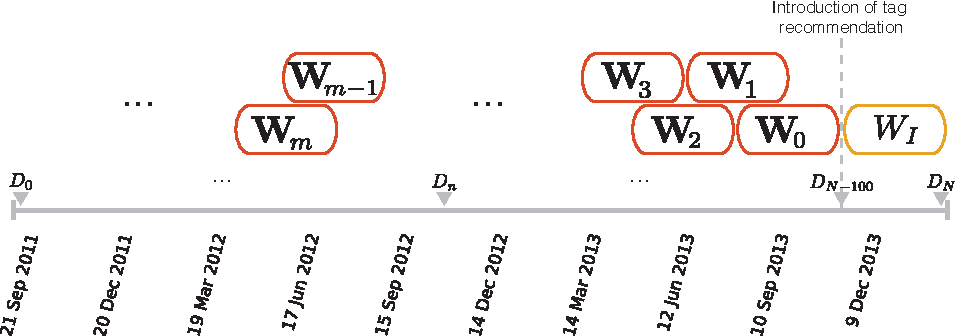
\includegraphics[width=1.0\columnwidth]{ch05_impact/pics/fig04_analysis_windows}}
\caption[Time period vectors and analysis windows]{Time period vectors $\daysVector$ and $\referenceWindowsVector$, and the analysis window of interest $\windowOfInterest$.}
\label{impact:fig:analysis_windows}
\end{figure}

As mentioned, we are interested in comparing the results of the defined metrics for time periods \emph{before} and \emph{after} the introduction of tag recommendation. In the case of metrics that are computed on a daily basis, we perform the comparison by computing the average of each metric over the range of days in $\mathbf{\daysVector}$ included in the window of interest $\windowOfInterest$ and in each reference window $\referenceWindowsVector_{m}$. Then, the average obtained from $\windowOfInterest$ is compared with the average obtained for each time period $\referenceWindowsVector_{m}$. This results in a total of $M$ comparisons per metric. In our results section, and unless stated otherwise, we always report the results of the comparison between $\windowOfInterest$ and the $\referenceWindowsVector_{m}$ that yields the minimum difference. Hence, our results only show the case in which the tag recommendation system has the least impact. For each one of these comparisons, we assess statistical significance by taking the daily results of the metric corresponding to the compared time periods $\windowOfInterest$ and $\referenceWindowsVector_{m}$ and performing the Mann-Whitney U test with a significance level of 0.01. For the case of metrics that are not computed on a daily basis, we follow different approaches for comparing and assessing statistical significance. These approaches  have been described for every particular metric in corresponding subsections of Sec.~\ref{impact:sec:definition_of_metrics}.

Our analysis data includes annotations for sounds of very different natures and from users with very different levels of expertise. During the analysis period, some users uploaded only one sound, while others uploaded thousands, with the average being on 12.7 uploaded sounds per user. % min:1, max:5655, avg: 12.69, med: 2, 75th perc: 7
A final point to note is that, although we do not perform any cleaning of the considered Freesound data, we remove from our consideration all tag applications performed by a specific user that, during a narrow time period within $\windowOfInterest$ (from 17 January 2014 to 27 January 2014), intensively uploaded and annotated sounds using three times more tags per sound than the average. We considered this user as being a clear outlier that could potentially bias the results of our analysis magnifying the observed impact of tag recommendation. %by significantly increasing the average tagline length after the introduction of tag recommendation.


%%%%%%%%%%%%%%%%%%%%%%%%%%%%%%%%%%%%%%%%%%%%%%%%%%%%%%%%%%%%%%%%%%%%%%%%%%%%%%%%%%%%%%%%%%%%%%%%%%%%%%%%%%%%%
\section{Results and discussion}
\label{impact:sec:results}


%%%%%%%%%%%%
\subsection{Vocabulary convergence}
\label{impact:sec:results_vocabulary_convergence}


\subsubsection{Percentage of new tags}
\label{impact:sec:percentage_of_new_tags_results}

\begin{figure}
\centerline{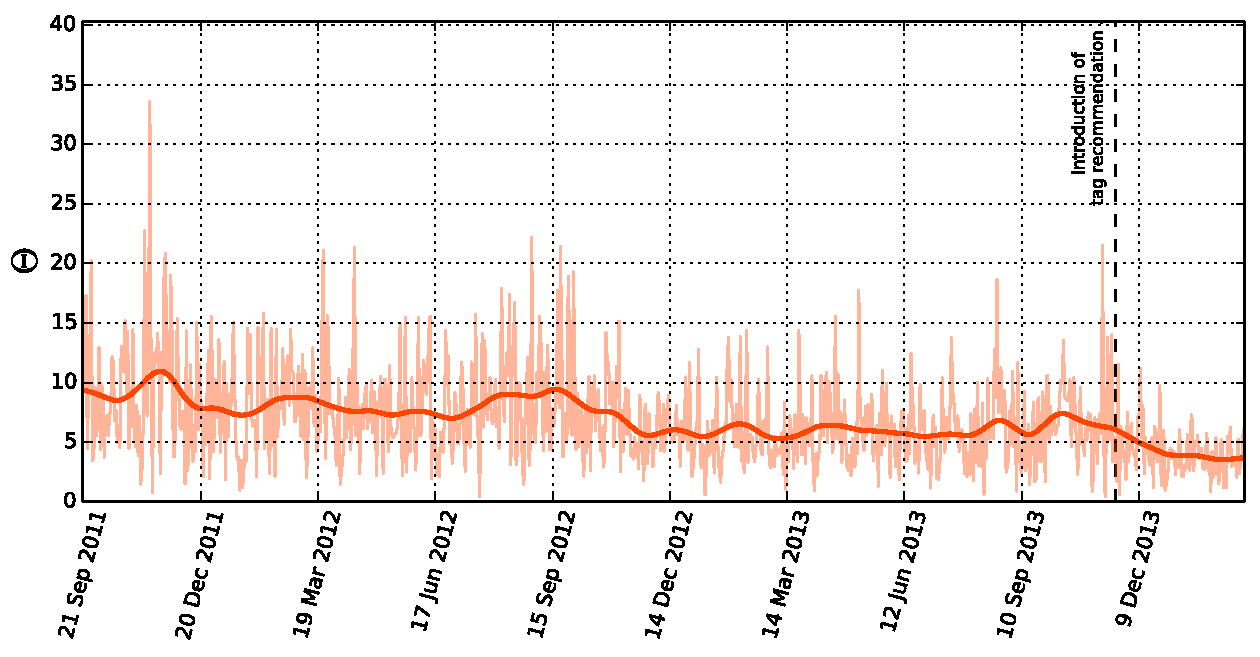
\includegraphics[width=\figSizeMax]{ch05_impact/pics/fig05_percentage_new_tags}}
\caption[Evolution of the percentage of new tags]{Evolution of the percentage of new tags $\metricVocabularyConvergence$. The thinner line corresponds to computed $\metricVocabularyConvergence$. The bold line corresponds to a smoothed version of $\metricVocabularyConvergence$. Smoothing is performed by convolution over a moving Hann window of 51 days. That particular number of days has been arbitrarily chosen to generate an informative yet visually appealing figure. Unless stated otherwise, the same smoothing strategy is applied in the other figures in this chapter.} 
\label{impact:fig:percentage_new_tags}
\end{figure}

Fig.~\ref{impact:fig:percentage_new_tags} shows the evolution of the percentage of new tags $\metricVocabularyConvergence$ over the considered time period. We see that, as expected, it qualitatively decreases after the introduction of tag recommendation. The minimum difference we observe between $\windowOfInterest$ and all $\referenceWindowsVector_m$ is a decrease of 1.7\%, which is found to be statistically significant ($\pvalue = 4.01\cdot 10^{-6}$). The maximum difference we observe is a decrease of 5\% ($\pvalue = 1.26 \cdot 10^{-15}$). 

The depicted evolution suggests an influence of the tag recommendation system on the percentage of new tags. However, looking at Fig.~\ref{impact:fig:percentage_new_tags}, a decreasing global trend can be qualitatively observed, even before the introduction of tag recommendation.
To compensate for the existence of such a trend, we perform an extra analysis in which we apply a correction to the $\metricVocabularyConvergence$ data points obtained from $\windowOfInterest$. The correction consists in computing a linear regression with all data points before the introduction of tag recommendation and then subtracting the linear projection of that trend to the data after the introduction of tag recommendation. Once we apply the correction to $\metricVocabularyConvergence$ over the window $\windowOfInterest$, we repeat the comparisons with all reference windows $\referenceWindowsVector_m$ and observe, this time, a minimum $\metricVocabularyConvergence$ decrease of 1.5\% which still remains statistically significant ($\pvalue = 5.68\cdot 10^{-5}$).
The observed global decreasing trend might be explained by a vocabulary consolidation process inherent to the tagging system, which is later accelerated with the introduction of tag recommendation.

It could be further argued that during the time period between 15 September 2012 and 14 December 2012 a localised decreasing pattern can also be observed with a similar strength to the one we observe after the introduction of tag recommendation. 
This decreasing pattern might be explained by the apparent local increase that can be observed in the previous months, which might be provoked by a particular user uploading a significant number of sounds with many new tags. Importantly, no relevant patterns can be observed in the other studied metrics during that particular period of time (see below). Moreover, just by simple observation of Fig.~\ref{impact:fig:percentage_new_tags}, it can be spotted that the variance of $\metricVocabularyConvergence$ is smaller after the introduction of tag recommendation, thus giving more relevance to the observed decreasing pattern during $\windowOfInterest$. 
As mentioned, it is the consideration of similar results from several different metrics that allows us to draw conclusions regarding the formulated hypotheses. 




\subsubsection{Average user vocabulary size}
Fig.~\ref{impact:fig:user_vocabulary_size} shows the evolution of the average user vocabulary size $\metricAverageVocabularySize$. In it, a clear impact of the tag recommendation system can be observed, as $\metricAverageVocabularySize$ consistently increases after the introduction of tag recommendation. When comparing results for the analysis window $\windowOfInterest$ and the other reference windows $\referenceWindowsVector_m$, we found a minimum $\metricAverageVocabularySize$ increase of 3.46 tags per user ($\pvalue = 2.303\cdot 10^{-11}$). 
This demonstrates that, after the introduction of tag recommendation, users tend to use a wider variety of tags as their vocabulary size is significantly increased.


\begin{figure}
\centerline{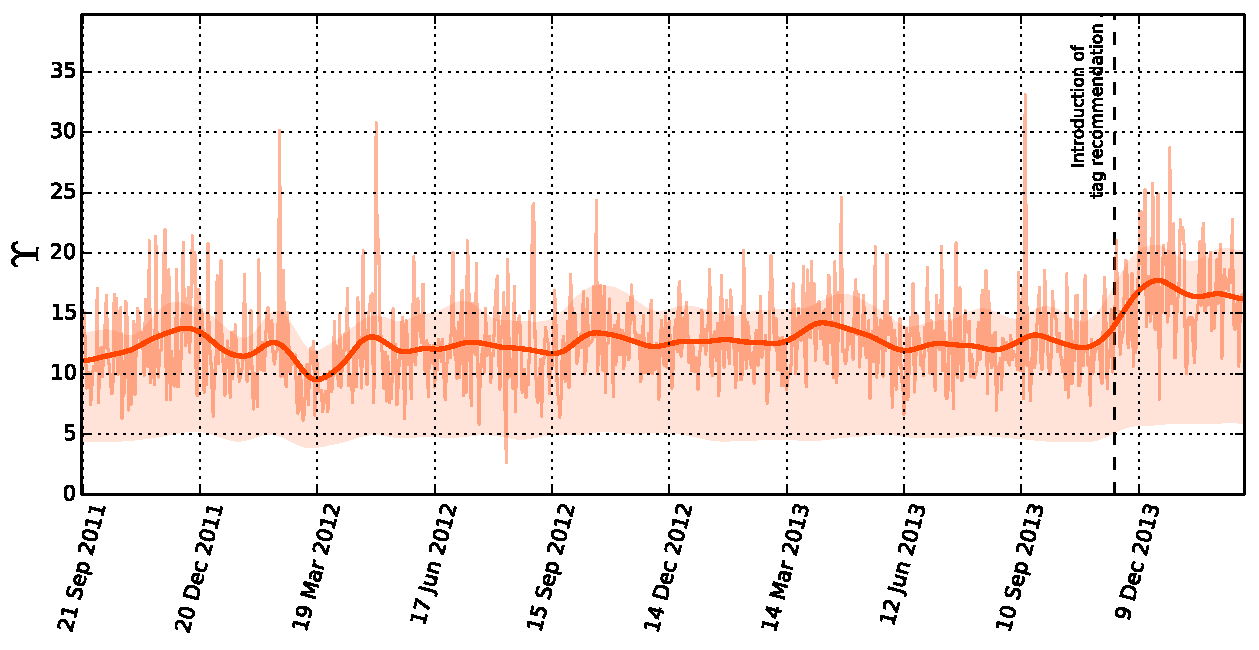
\includegraphics[width=\figSizeMax]{ch05_impact/pics/fig06_user_vocabulary_size}}
\caption[Evolution of average user vocabulary size]{Evolution of average user vocabulary size $\metricAverageVocabularySize$. The thinner line corresponds to computed $\metricAverageVocabularySize$. The bold line corresponds to a smoothed version of $\metricAverageVocabularySize$. The filled area shows the range between the lower and upper quartiles of the original data. 
}
\label{impact:fig:user_vocabulary_size}
\end{figure}


\subsubsection{User vocabulary sharing}
\label{impact:sec:vocabulary_sharing_users}
% 73240/1148 = 63.79
% 122474/1335 = 91.74
As described in Sec.~\ref{impact:sec:definition_of_metrics}, to analyse user vocabulary sharing ($\metricUserVocabularySharing$) we built two networks using data before and after the introduction of tag recommendation.
In particular, we use data from the analysis windows $\referenceWindowsVector_0$ and $\windowOfInterest$, respectively. The resulting network built with data from $\referenceWindowsVector_0$ has a total of 1,148 nodes (i.e.,~users) and 73,240 edges (yielding a ratio of 63.79 edges per node), whereas the network built with data from $\windowOfInterest$ features 1,335 nodes and 122,474 edges (91.74 edges per node). Just by looking at these numbers, it can already be seen that users in the $\windowOfInterest$ network are much more connected among them. Fig.~\ref{impact:fig:users_graph_strength} shows the complementary cumulative node strength distribution of the two networks. The distribution shows that, for a given probability, the network after the introduction of tag recommendation features nodes with a higher strength. Comparing the two distributions yields a statistically significant $\metricUserVocabularySharing$ increase of 2.12 ($\pvalue = 8.652\cdot 10^{-17}$). 
These observations highlight that the tag recommendation system effectively favours tags sharing among users. 

\begin{figure}
\centerline{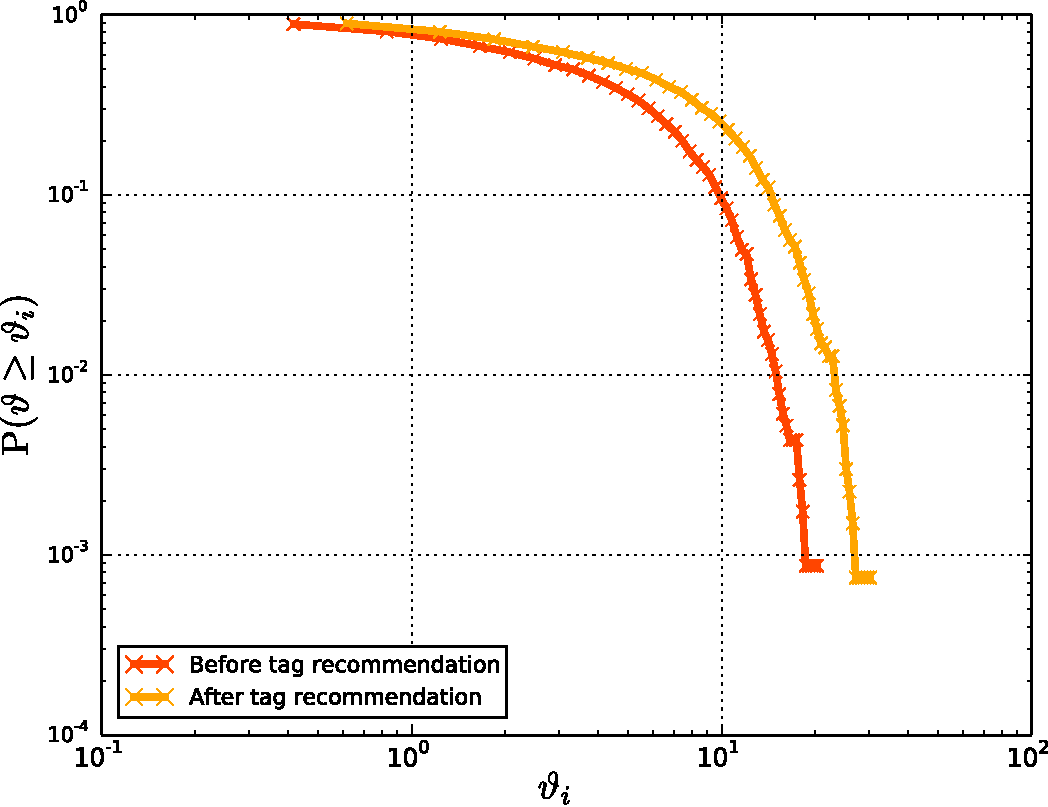
\includegraphics[width=0.66\columnwidth]{ch05_impact/pics/fig07_users_graph_strength}}
\caption[Complementary cumulative node strength distribution of user-user network]{
Complementary cumulative node strength $\nodeStrength$ distribution of user-user network $\usersNetwork$ before and after the introduction of tag recommendation. Networks are build with data from analysis windows $\referenceWindowsVector_0$ and $\windowOfInterest$ respectively.}
\label{impact:fig:users_graph_strength}
\end{figure}


\subsubsection{Sound vocabulary sharing}
% 3414449/9898 = 344.97 abans
% 7405037/12946 = 571.99 dps
The analysis of sound vocabulary sharing $\metricSoundVocabularySharing$ reports similar results to those of user vocabulary sharing. The resulting network built with data from $\referenceWindowsVector_0$ has a total of 9,898 nodes (i.e.,~sounds) and 3,414,449 edges (yielding a ratio of 344.97 edges per node), whereas the network built with data from $\windowOfInterest$ features 12,946 nodes and 7,405,037 edges (571.99 edges per node). Again, it can already be observed that the network after tag recommendation is much more connected. Fig.~\ref{impact:fig:sounds_graph_strength} shows the complementary cumulative node strength distribution of the two networks. In this case, we also observe an statistically significant overall increase of node strengths after the introduction of tag recommendation. Interestingly, this is somewhat more relevant in the range of sounds that used to be less connected in the network (roughly for $\nodeStrength < 200$). The average $\metricSoundVocabularySharing$ increase is of 34.26 ($\pvalue = 2.606\cdot 10^{-231}$). This result is consistent with what we find in the case of user vocabulary sharing.

\begin{figure}
\centerline{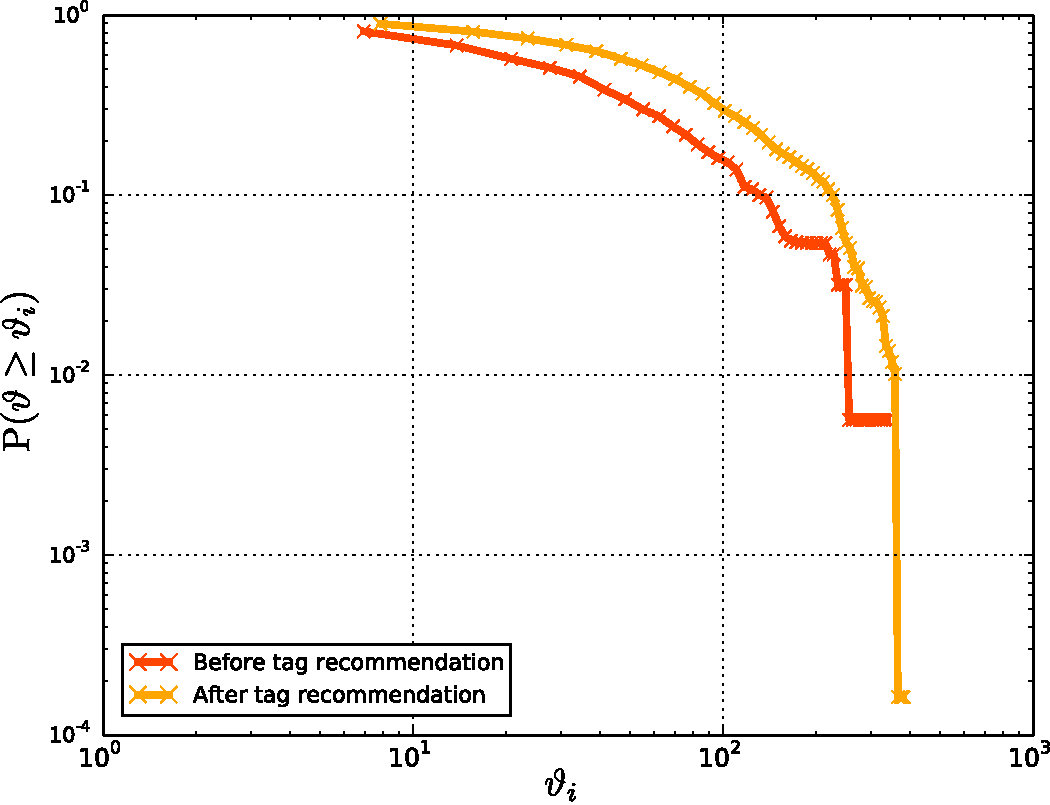
\includegraphics[width=0.66\columnwidth]{ch05_impact/pics/fig08_sounds_graph_strength}}
\caption[Complementary cumulative node strength distribution of sound-sound network]{
Complementary cumulative node strength $\nodeStrength$ distribution of sound-sound network $\soundsNetwork$ before and after the introduction of tag recommendation. Networks are build with data from analysis windows $\referenceWindowsVector_0$ and $\windowOfInterest$ respectively.}
\label{impact:fig:sounds_graph_strength}
\end{figure}


\subsubsection{Discussion}

We have seen that the tag recommendation system lessens the invention of new tags and that, at the same time, it increases the size of users' vocabulary and the number of tags that are shared among users and sounds. Thus, we can conclude that all users annotating sounds receive a common influence that positively affects the convergence of the vocabulary in the folksonomy by leveraging the reuse of tags, reducing the generation of new ones, and increasing the number of distinct tags in users' personal vocabulary.

We have also found that both user and sound vocabulary sharing are increased after the introduction of tag recommendation. This observation, combined with the increase in users' vocabulary size, leverages the value of sound annotations. It reveals a better agreement on the vocabulary of tags used to annotate sounds and also an increase of its size. Therefore, sounds are described using a more coherent and complete vocabulary.


%%%%%%%%%%%%
\subsection{Quality of annotations}
\label{impact:sec:results_quality_annotations}


\subsubsection{Average tagline length}
\label{impact:sec:length_of_tagline}

Fig.~\ref{impact:fig:length_of_tagline} shows the evolution of the average tagline length $\metricAverageTaglineLength$. We observe a clear increase after the introduction of tag recommendation. Comparing results for the analysis window $\windowOfInterest$ and reference windows $\referenceWindowsVector_m$, we observe a minimum $\metricAverageTaglineLength$ increase of 1.32 tags per sound ($\pvalue = 7.553\cdot 10^{-6}$). 
Similarly to what we noted in Sec.~\ref{impact:sec:percentage_of_new_tags_results}, Fig.~\ref{impact:fig:length_of_tagline} seems to show a global increasing tendency already before the introduction of tag recommendation. We repeated the same extra analysis of that section (i.e.,~computing the linear regression of data before the introduction of tag recommendation and correcting $\metricAverageTaglineLength$ in $\windowOfInterest$ with the linear projection of the trend) and still observed a statistically significant minimum $\metricAverageTaglineLength$ increase of 1.22 tags per sound ($\pvalue = 3.65\cdot 10^{-5}$). Considering the average tagline length for the time periods before and after the introduction of tag recommendation, the observed increase means that sounds are annotated with approximately 20\% more tags when users are influenced by the tag recommendation system. This observation is also supported by looking at the histogram of tagline lengths before and after the introduction of tag recommendation (Fig.~\ref{impact:fig:length_of_tagline_distribution}). The increase of the average tagline length suggests that annotations performed using the recommendation system are more comprehensive and, presumably, of better quality than annotations performed without the recommendation system. 

\begin{figure}
\centerline{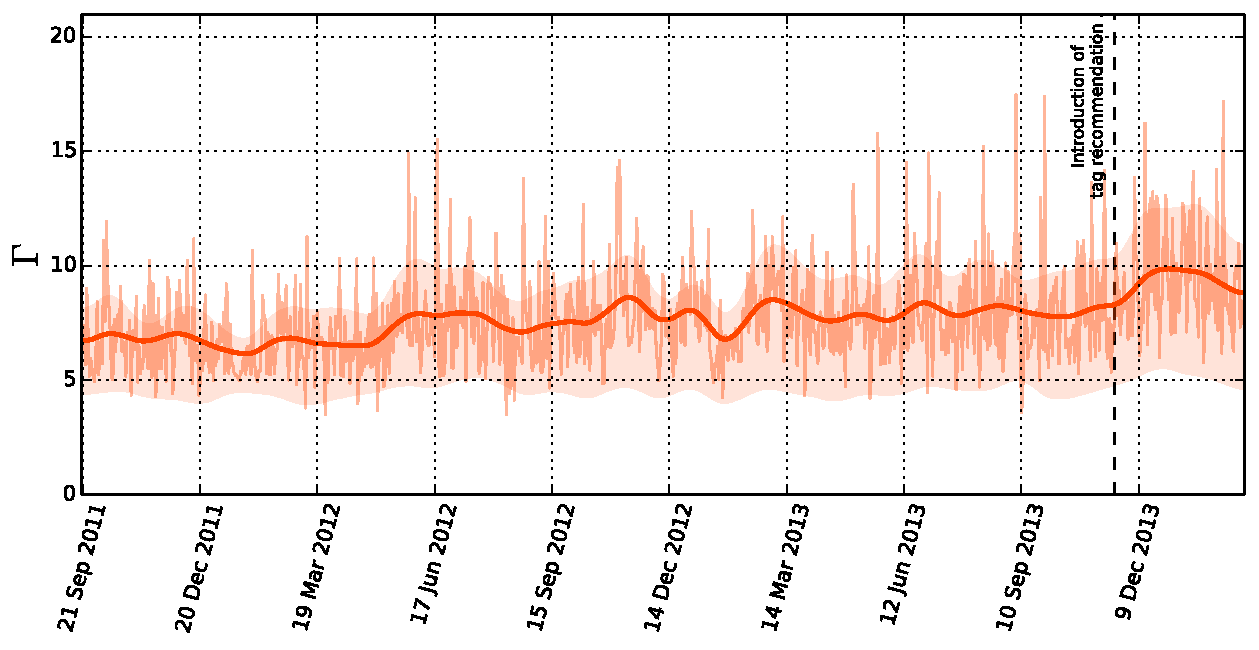
\includegraphics[width=\figSizeMax]{ch05_impact/pics/fig09_length_of_tagline}}
\caption[Evolution of average tagline length]{Evolution of average tagline length $\metricAverageTaglineLength$. The thinner line corresponds to computed $\metricAverageTaglineLength$. The bold line corresponds to a smoothed version of $\metricAverageTaglineLength$. Filled area shows the range between the lower and upper quartiles of the original data.}
\vspace{0.8cm}
\label{impact:fig:length_of_tagline}
\end{figure}

\begin{figure}
\centerline{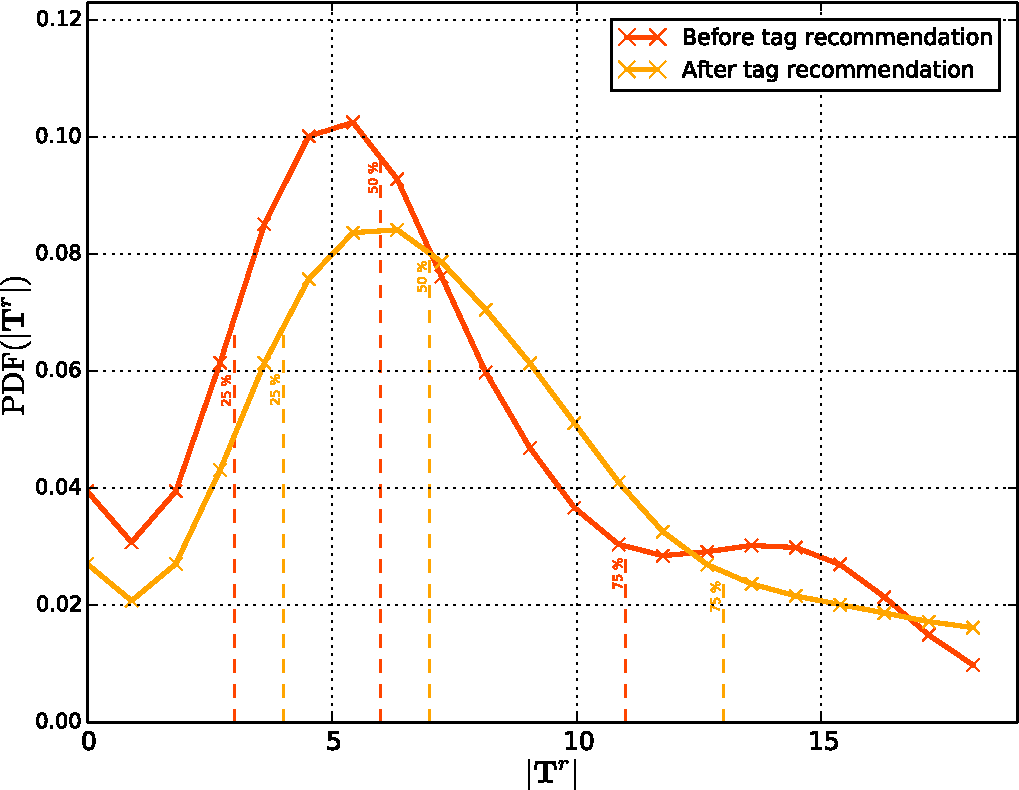
\includegraphics[width=0.7\columnwidth]{ch05_impact/pics/fig10_length_of_tagline_histogram}}
\caption[Probability density function of tagline lengths]{Probability density function of tagline lengths $|\tagsOfSoundR|$ before and after the introduction of tag recommendation. Data is drawn from the analysis windows $\referenceWindowsVector_0$ and $\windowOfInterest$, respectively. Smoothing is performed using an arbitrarily chosen Hann window of 11 points. Dashed vertical lines with attached percentage values indicate the percentage of sounds whose tagline length is less than or equal to what is indicated in the corresponding line position.}
\label{impact:fig:length_of_tagline_distribution}
\end{figure}


\subsubsection{Percentage of misspelled tag applications}
\label{impact:sec:misspelled_tag_applications}

Fig.~\ref{impact:fig:misspelled_tag_applications} shows the evolution of misspelled tag applications $\metricMispellings$. 
As expected, we observe a slight decreasing tendency in $\metricMispellings$ after the introduction of tag recommendation
When comparing results for the analysis window $\windowOfInterest$ and the other reference windows $\referenceWindowsVector_m$, we find a minimum $\metricMispellings$ decrease of 1.4\% (not statistically significant), and a maximum decrease of 5\% (statistically significant, with $p = 4.775\cdot 10^{-5}$). 
Hence, this shows that the introduction of tag recommendation has a moderate impact on misspelled tags, helping users to generate up to 5\% less tags with misspellings.

\begin{figure}
\centerline{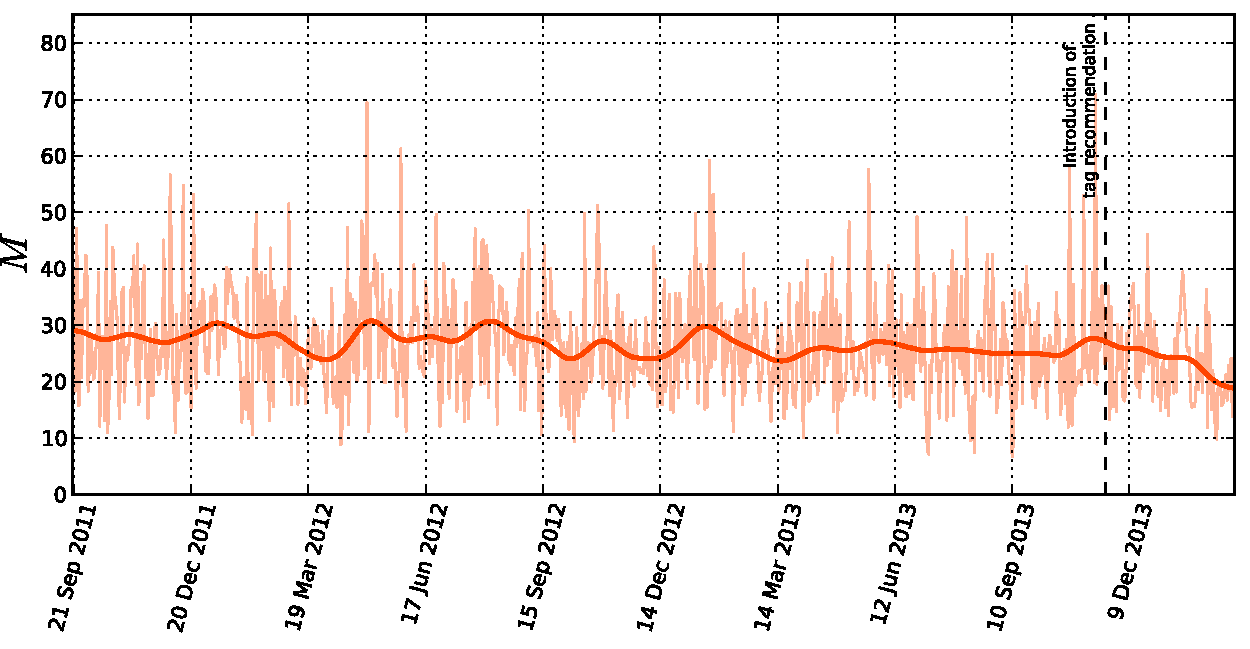
\includegraphics[width=\figSizeMax]{ch05_impact/pics/fig99_misspelled_tag_applications}}
\caption[Evolution of the percentage of misspelled tag applications]{Evolution of the percentage of misspelled tag applications $\metricMispellings$. Similarly to the previous figures, the thinner line corresponds to computed $\metricMispellings$. The bold line corresponds to a smoothed version of $\metricMispellings$.
}
\label{impact:fig:misspelled_tag_applications}
\end{figure}



\subsubsection{Tag frequency distribution} 

Fig.~\ref{impact:fig:tag_frequency_distribution} shows the complementary cumulative tag frequency distribution before and after the introduction of tag recommendation. It can be observed that the distribution after the introduction of tag recommendation tends to be more even, particularly reinforcing the usage of tags in the low and mid frequency ranges (tags with less than 800 occurrences). This means that less popular tags gain importance after the introduction of tag recommendation. Less popular tags typically correspond to narrower semantic concepts, which are used to bring more details to sound annotations. Again, this observation is consistent with previous observations regarding vocabulary convergence. It reflects an increase in both user and sound vocabulary sharing, as tags with less frequency gain importance and start being more widely used. It also suggests that annotations after the introduction of tag recommendation are more detailed as the usage of tags in the low and mid frequency ranges is reinforced.

To complement these results, we evaluated how well tag frequency distributions corresponding for the analysis windows $\referenceWindowsVector_0$ and $\windowOfInterest$ fit into a power law distribution. In both cases, the analysis shows a better fit for a log-normal distribution rather than a power law distribution. However, the tag frequency distribution after the introduction of tag recommendation shows a better fit for the power law than the distribution before tag recommendation, which may also suggest the presence of a better converging vocabulary yielding more meaningful descriptions (Sec.~\ref{impact:sec:methods_quality_of_annotations}).%\citep{Mathes2004,Cattuto2006,halpin2006,Wagner2014}.


\begin{figure}
\centerline{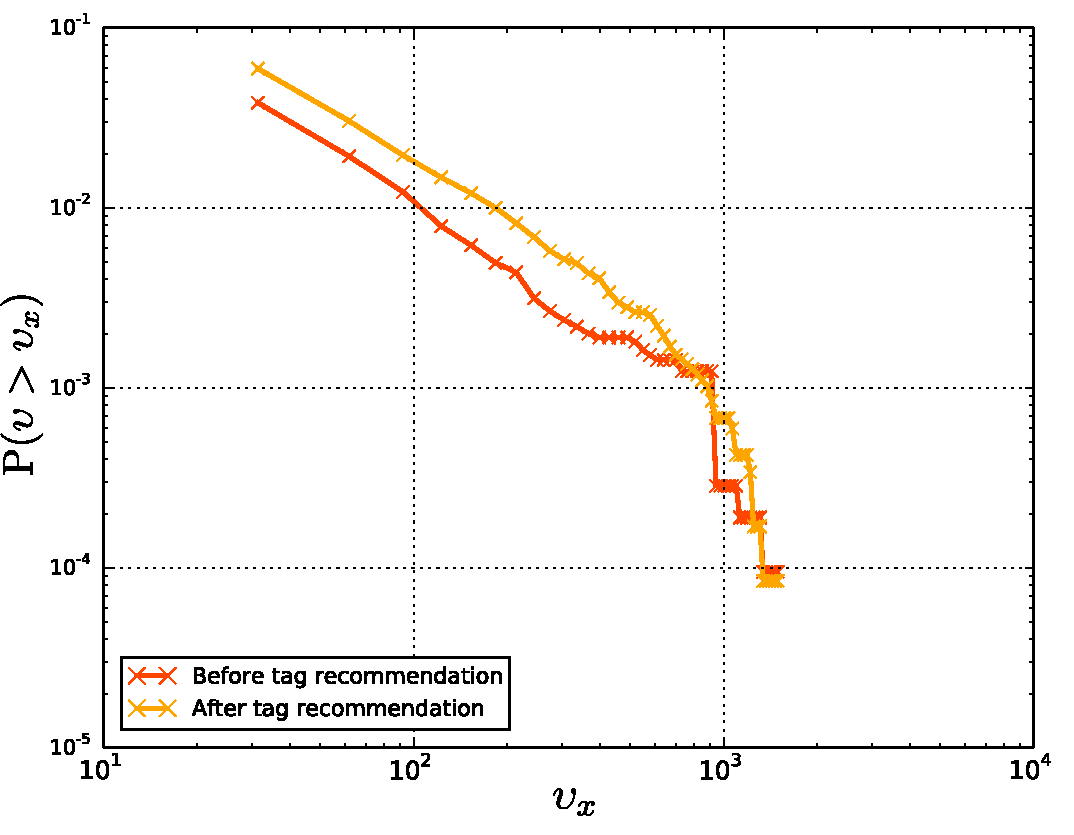
\includegraphics[width=0.7\columnwidth]{ch05_impact/pics/fig11_tag_frequency_distribution}}
\caption[Complementary cumulative tag frequency distribution]{Complementary cumulative tag frequency $\tagFrequency$ distribution before and after the introduction of tag recommendation. Data is drawn from the analysis windows $\referenceWindowsVector_0$ and $\windowOfInterest$, respectively. }
\vspace{0.8cm}
\label{impact:fig:tag_frequency_distribution}
\end{figure}


\subsubsection{Subjective annotation quality} 
We analyse the results of the online experiment described in Sec.~\ref{impact:sec:methods_quality_of_annotations} and observe a subjective annotation quality of $\metricQualitativeAnnotationQuality=0.075$ (0.81 standard deviation). One third of the quality judgements performed by the participants correspond to ``No preference'' judgements ($\unionOfQualityJudgements_j=0$). If we discard these judgements, the subjective annotation quality is increased to $\metricQualitativeAnnotationQuality=0.114$ (0.99 standard deviation), meaning that in 55\% of the judgements the sounds described using the tag recommendation system are considered to be better annotated. These results indicate that participants in the experiment have a slight tendency to consider annotations of sounds described using the tag recommendation system as being better than annotations of sounds made without the tag recommendation system.
To further validate these results, we computed Cohen's kappa coefficient to measure the agreement among the quality judgements performed by the participants in the experiment~\citep{carletta1996assessing}. 
After all possible pairwise comparisons between the different participants in the experiment, we observe an average kappa coefficient of 0.22. Thus, participants in the experiment tend to agree in their judgements. This reinforces our previous observations.

During the experiment, participants also provided textual comments about some of their quality judgements. In general, participants used comments to explain the reason why they considered sounds to be badly annotated. Among these reasons, the most common ones are the presence of misleading or uncompleted annotations, the presence of tags not related to the sound being annotated, and the presence of tags with typographical errors. In the participants' sample, all these reasons are reported evenly for sounds uploaded before and after the introduction of tag recommendation.


\subsubsection{Discussion}
We have seen that the average number of tags used to annotate a sound is larger after the introduction of tag recommendation. 
A similar observation is made in a study by~\cite{Ames2007}, in which two mobile phone applications for uploading photos to Flickr are compared. One of the applications features a tag recommendation system to aid users in the tagging process, and an increase in the average tagline length is observed for those photos uploaded with that application.

The fact that the average tagline length increases after the introduction of tag recommendation also reinforces the previously discussed observations regarding vocabulary convergence. Tag recommendation yields more tag applications and potentially more comprehensive sound annotations, and yet fewer new tags are created while vocabulary sharing is increased. Hence, our results indicate that sound annotations after the introduction of tag recommendation are done using a more coherent and complete vocabulary of tags. This fact seems to be further confirmed by the results of the online experiment we set up to analyse qualitative annotation quality, as participants on this experiment preferred annotations of sounds uploaded after the introduction of tag recommendation.

The tag frequency distribution we observe after the introduction of tag recommendation also supports the increase in the convergence of the vocabulary. 
In this case, a better agreement is reached specially for those tags with lower frequencies of occurrence. Thus, we could say that there is a better agreement on the tags users choose to annotate specific concepts, which leverages the value (and thus the quality) of the annotations.

Finally, we also observed that tag recommendation helps users in slightly reducing misspellings in the tags they introduce. This also supposes an improvement in the quality of annotations. However, the impact we observe is rather limited, which may be explained by several factors. Firstly, the way in which we estimate misspelled tags is not perfectly accurate and thus some noise is present in the metric (see Sec.~\ref{impact:sec:methods_quality_of_annotations}). Secondly, the nature of the tag recommendation system does not prevent itself from actually recommending tags with misspellings. Hence, even if it is intuitively less likely that misspelled tags will feature a strong similarity with any of the input tags, it is still possible that these are recommended. 
Finally, we can only expect tag recommendation to effectively help in reducing misspellings for the tags that are actually suggested by the system and correctly predicted. As we describe below in Sec.~\ref{impact:sec:percentage_correcly_predicted_tags_results}, approximately 19\% of the tags of a tagline are correctly predicted, and this can be taken as a rough estimate of an upper bound for the decrease in the percentage of misspelled tag applications. Furthermore, even when relevant tags are recommended by the system and are correctly predicted, many users still prefer to manually type them instead of clicking on the list of suggestions, which may still lead to misspellings (see Sec.~\ref{impact:sec:percentage_correcly_predicted_tags_results}).
That being said, overall results regarding the quality of annotations suggest that the introduction of tag recommendation has a moderate yet positive impact on this aspect.


%%%%%%%%%%%%
\subsection{Cost of the annotation process}
\label{impact:sec:cost_annotations}


\subsubsection{Average tag application time}

Fig.~\ref{impact:fig:tag_time} shows the probability density function of the average time per tag application $\metricAverageTagApplicationTime$ with and without the use of the tag recommendation system. Even though we observe a small average decrease in $\metricAverageTagApplicationTime$ for annotation sessions using the tag recommendation system, it is found to be not statistically significant ($\pvalue = 0.83$). This means that no substantial difference on the time needed to perform a tag application can be reported. However, if we look at the total amount of time invested in annotating every sound (instead of every tag), we do observe a statistically significant average increase of roughly 35 seconds per sound after the introduction of tag recommendations ($\pvalue = 6.2\cdot 10^{-3}$), which represents an increase of approximately 20\%. This is consistent with the 20\% increase of the tagline length we observed in Sec.~\ref{impact:sec:length_of_tagline}. Thus, in general, we could say that users need at least the same amount of time to perform a single tag application as they needed before using the system. However, annotations are longer and therefore users spend more time annotating sounds.

\begin{figure}
\centerline{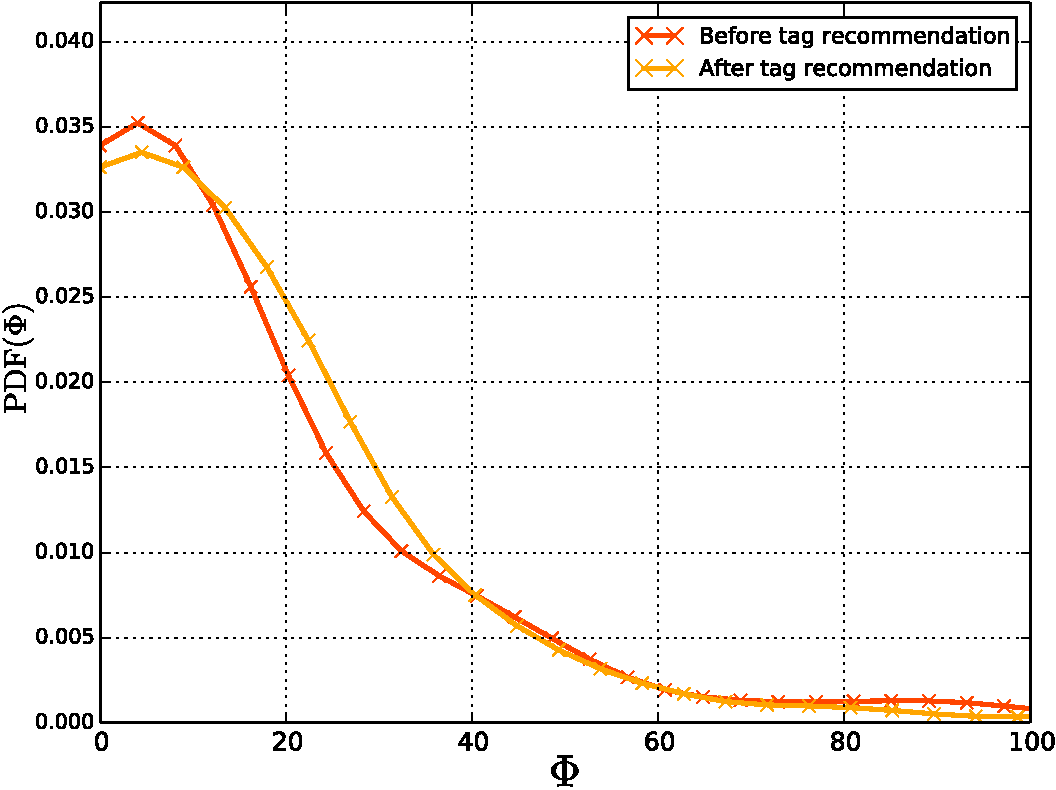
\includegraphics[width=0.7\columnwidth]{ch05_impact/pics/fig12_time_pdf}}
\caption[Probability density function of the average tag application time]{Probability density function of the average tag application time $\metricAverageTagApplicationTime$ with and without the tag recommendation system. Curves are smoothed using a Hann window of 11 points.}
\label{impact:fig:tag_time}
\end{figure}


\subsubsection{Average number of correctly predicted tags}
\label{impact:sec:percentage_correcly_predicted_tags_results}

As explained in Sec.~\ref{impact:sec:definition_of_metrics}, the average number of correctly predicted tags $\metricPercentageOfCorrectlyPredictedTags$ can only be computed with data drawn from $\windowOfInterest$. Computing it on a daily basis shows that an average of 2.10 tags (from those finally assigned to sounds) were suggested by the recommendation system. This corresponds to approximately 19\% of tags in a tagline. This is similar to what we found in Chapter~\ref{sec:class} (Table ~\ref{tab:results_general_ub}), in which an average of 2.41 tags were correctly predicted by the class-based tag recommendation method (corresponding to approximately 29\% of the tags in a tagline). 
%The bigger difference between both numbers of correctly predicted tags when expressed as a percentage can be explained because the average tagline length was lower in the experiment performed in Chapter~\ref{sec:class} as compared to the current experiment.%7.4
Hence, according to these results, the tag recommendation system behaves similarly both in the real-world and in a controlled environment, with a certain tendency of users accepting fewer tags in the real world.

Among the correctly predicted tags, we make a distinction between those that are added to the tagline by users clicking on the corresponding tag in the list of suggestions, and those that are manually typed by users. If we only consider the tags that are added to the tagline by users actively clicking on the suggestion, we observe an average number of 1.58 correctly predicted tags, corresponding to approximately 13\% of the tags in a tagline. This suggests that, in many occasions, users still prefer to manually type the tags instead of switching to the mouse and clicking on the list of suggestions.
In general, these results show that, even though an important part of the final tagline for a sound can be constructed using tags suggested by the recommendation system, the majority of these tags have to be generated by users themselves, and are not necessarily related with those suggested by the system.
%This also partially explains why the impact on the average time per tag application we reported above is rather minimal, although in any case it is not clear whether the act of clicking on the list of suggestions would require less time than manually typing the tag.


\subsubsection{Discussion}
\label{impact:sec:cost_annotation_process_discussion}
Contrary to what we expected, we have observed that the tag recommendation system does not seem to have a significant impact on the cost of the annotation process. 
Although we have seen that users need significantly more time to annotate individual sounds when using the tag recommendation system, we have also seen that this increase can be attributed to the proportional increase of the average tagline length. Hence, the actual time required for every individual tag application does not significantly change.
Furthermore, we observed that most of the tags assigned to sounds are not drawn from the list of recommended tags, meaning that most of the annotation process still consists of a generation process where users create tags from scratch rather than a recognition process where users validate tags from a list of suggestions.
 
There are several potential reasons why we do not observe the expected impact on the cost of the annotation process.
On the one hand, we observed that only 13\% of the tags in taglines are added from the list of suggestions by actually clicking on them. Hence, assuming that it is faster to click on tags rather than to manually type them (which is probably not always true), the impact we can expect on the time required for introducing tags should be lower than that 13\%.
Also, it seems intuitively plausible that users need more time to generate the tags (or recognise them from a list) than to actually introduce them. Hence, the potential impact of lessening the time required for introducing tags is further reduced.
On the other hand, the impact of the recommendation system is again limited by the fact that most of the introduced tags are not drawn from system recommendations, and thus an important part of the annotation process does not significantly change after the introduction of tag recommendation. In fact, our results might be suggesting that the cost of the recognition process is not actually lower than the cost of the generation process. This also seems reasonable, as the union of all recommended tags for a given sound is much larger than the length of the actual tagline (i.e., new tags are recommended every time that a tag is added to the tagline, see Sec.~\ref{impact:sec:tag_rec_interface}). Therefore, the recognition process must operate over a large set of tags. 

Finally, we believe that our metrics regarding the cost of the annotation process are highly dependent on the particular interface of the recommendation system. Also, the recommendation interface can have different impacts according to how users adapt to it.
Unfortunately, our analysis does not contain data to be compared coming from other recommendation interfaces. 
However, to get some more insight into that aspect, we repeated the calculations of the average tag application time but this time considering experienced and non-experienced users separately. We divided users according to the number of sounds they uploaded during our analysis period. In particular, we set the threshold at the third quartile of the distribution of uploaded sounds per user, which corresponds to 7 uploaded sounds. What we observe is that the average tag application time after the introduction of tag recommendation increases for non-experienced users and decreases for experienced users by a similar amount of about 3 seconds per tag application ($p = 2.15\cdot 10^{-3}$ and $p = 3.65\cdot 10^{-3}$, respectively). 
This shows that experienced users were able to take advantage of the recommendation interface and generate annotations slightly faster, but it also shows that the interface had a negative impact on non-experienced users, apparently increasing the cost of the annotation process.
This could be explained because experienced users probably have a better understanding of the tagging process and can easily interpret and take advantage of tag recommendation.
Nevertheless, we think that to draw more consistent conclusions regarding the impact of tag recommendation on the cost of the annotation process, further research should be carried out.


%%%%%%%%%%%%%%%%%%%%%%%%%%%%%%%%%%%%%%%%%%%%%%%%%%%%%%%%%%%%%%%%%%%%%%%%%%%%%%%%%%%%%%%%%%%%%%%%%%%%%%%%%%%%%

\section{Conclusion}
\label{impact:sec:conclusion}

In this chapter we have analysed the impact of a state of the art tag recommendation system into the real-world folksonomy of a large-scale sound sharing platform, Freesound. After a the review of current related work done in Chapter~\ref{sec:SOA} (Sec.~\ref{sec:soa:impact_tag_recommendation}), we have identified three main hypotheses regarding the impact that such a system should have when introduced into a tagging system, and we have defined several reusable metrics to evaluate that impact. We have analysed data comprising of a period from 21 September 2011 to 28 February 2014, the last three months of which correspond to data after the introduction of tag recommendation. To the best of our knowledge, these kind of quantitative analyses have not been done before using large-scale data from a real-world folksonomy. Hence, no empirical assessment of the three identified hypotheses was available to date. %The definition of several necessary metrics to assess the three hypotheses is also a further contribution of this chapter.

Our results show a significant impact of tag recommendation into most of the metrics we defined. However, the result of a single metric in isolation is probably not entirely relevant in our analysis. Instead, the fact that we observe how the changes on several metrics can be explained by some of the outlined hypotheses gives a particular value to our analysis. Overall we observe that the first hypothesis (regarding vocabulary convergence) is clearly validated, that the second one (regarding the quality of annotations) only seems to be partially validated, and the third one (regarding the cost of the annotation process) does not seem to be validated.  However, we believe the latter is particularly dependent on the annotation interface, and that its impact could be greatly improved by designing an interface specifically focused on reducing the cost of the annotation process.

Although in this work we only analyse data in the context of Freesound, we believe that our results are, to some extent, indicative of the impact that tag recommendation can potentially have in other tagging systems.
However, tagging systems of different nature may react differently to the introduction of a tag recommendation system.
An important aspect here is to take into account the motivations that users have for tagging their resources.
In narrow folksonomies such as Freesound and Flickr, users typically tag their content so that other users (and also themselves) can easily find it in the future. However, resources are only annotated once, and therefore the tags added by the uploader of a resource should also be meaningful to other users of the platform. Contrarily, in broad folksonomies such as Delicious and CiteULike, resources are tagged multiple times by several users, and thus the main motivation for tagging is users' self organisation of the content, without necessarily considering the global context of the sharing platform (Secs.~\ref{soa:user_motivations} and~\ref{soa:types_of_tags}). 
As a result, very different tagging styles can arise because of the particularities of these two kinds of tagging systems.
The tag recommendation system that we use here is designed for narrow folksonomies. It does not try to personalise recommendations to particular users' tagging behaviours, but instead it learns from parts of the folksonomy on the basis of five audio classes (Sec.~\ref{class:sec:class_based_tag_rec_ref}).
Hence, we expect it to have a bigger impact in tagging systems featuring narrow folksonomies, where the more uniform across users a tagging style is, the better the platform becomes in providing content to other users.

Importantly, the metrics and analysis methodology described here are applicable to other collaborative platforms either featuring broad or narrow folksonomies. To further assess the validity of our results, an analysis with data coming from other tagging systems and tag recommendation systems should be performed. The main obstacle for carrying out this analysis is the limited availability of comprehensive tagging data, including annotations performed \emph{with} and \emph{without} the use of a tag recommendation system, and that comprise user activity for as long a period of time as the the one we analysed.

There are several aspects of the data we already collected that could be further researched to gain more insight into the impact of the tag recommendation system. 
Firstly, we do not perform any study of the generated taglines at the semantic level. By applying techniques for mapping tags to semantic concepts or categories~\citep[e.g.,][]{cantador2010}, we could analyse the impact of the recommendation system at the semantic level, and see if it effectively shapes tagging behaviour to a more extensive usage of particular kinds of tags such as content-related or self-organisational tags. Similarly, it could be further studied if other typical problems of tagging systems such as synonymy or polysemy are in fact affected by the use of a recommendation system.
Secondly, in the current work we just introduced the concept of user experience when analysing our results in Sec.~\ref{impact:sec:cost_annotation_process_discussion}. It would be interesting to further investigate this aspect by analysing the impact of the recommendation system to other evaluation metrics when considering users with different levels of expertise.
Thirdly, another way in which the current analysis could be further developed would be with the use of network analysis techniques to inspect the user-user and sound-sound networks built on the basis of shared tags. Using such analysis, it would be interesting to evaluate the existence of community structure in those networks and to see how potential communities in both networks might be related. For example, we could investigate if there are strongly connected communities of users that annotate sounds with a particular tagging style, and then see how the introduction of tag recommendation would affect those communities.

In our opinion, the biggest future challenge in tag recommendation is the design of systems that have a bigger impact on the quality of annotations. Annotations are very subjective and difficult to evaluate. However, a recommendation system could be designed to particularly focus on that issue by driving recommendations at higher semantic levels, for example being able to select candidate tags for recommendation in terms of variety and coverage of different semantic facets. 
In order for tag recommendation systems to have a deeper impact in the tagging behaviour and in the quality of annotations, we probably need to evolve the basic tag recommendation methods into \emph{assistive} processes where we can better guide users during the annotation process. % by having more knowledge about the semantics of our tags and the particular domain we are recommending tags for. 
%We foresee that one interesting research direction is the use of ontologies to drive future tag recommendation/assistive tagging systems. Such ontologies should embed knowledge about the domain for which we are recommending tags, including relations between tags and even organising tags into different categories regarding the kind of semantic information they are describing about the resources being annotated.
In the following chapter (Chapter~\ref{sec:ontology}), we explore this perspective by proposing an extension of the current class-based tag recommendation method which takes advantage of a domain-specific ontology to drive the recommendation process.



\cleartorecto%!TEX root = ../thesis_a4.tex

\chapter[A new perspective: ontology-based tag recommendation][A new pers.: ontology-based tag rec.]{A new perspective: ontology-based tag recommendation}
\label{sec:ontology}

\section{Introduction}
\label{sec:ontology:introduction}
%It is important to clarify that the focus of our exploratory research is not that much in the design and definition of the ontology, as its application in a tag recommendation system.

In this chapter we present a new perspective on tag recommendation systems and explore how can it tackle some of the tagging issues that have been identified in the previous chapters. 
The goal is to design a tag recommendation system that further improves the quality of resource annotations. 
In particular, the recommendation system is focused on helping users to generate more comprehensive, coherent and semantically meaningful resource annotations.
%For this purpose, we incorporate several ideas proposed by different authors in the tagging literature. 

A particularity of the folksonomies emerging from tagging systems is that tags are organised in a flat hierarchy, typically detached from a uniquely identifiable semantic meaning~\citep{golder2006,halpin2006}. Hence, tags are not restricted to a predefined set of concepts or a fixed vocabulary.
We have seen that this has the advantage of enabling a certain flexibility and ease of use from the users' point of view (Sec.~\ref{sec:SOA:tagging_systems}).
This is one of the reasons why  tagging systems have succeeded as a popular organisation system in online sharing platforms~\citep{shirky2005ontology,halpin2006,Cattuto2006}. 
However, we have also seen that this approach presents some disadvantages because different tagging conventions may coexist in a single folksonomy, and because the semantic meaning of tags can not be unambiguously determined (Sec.~\ref{soa:tagging_problems}).

The flexibility of user-generated folksonomies is often opposed to the accurateness and rigidity of \emph{ontologies}, which are designed by domain experts.
Ontologies provide, for a given domain, an unambiguous formalisation of its concepts, entities and their relations. 
Hence, where folksonomies feature free-form textual labels with no predefined semantic meaning, ontologies feature detailed concept hierarchies interlinked with semantically meaningful relations.
%These concepts are defined as a hierarchy of classes in the ontology, with object properties that define possible relations between instances (or individuals) of these classes.

Although folksonomies and ontologies appear to be opposed ways in which knowledge can be represented, some authors suggest that these are, in fact, complementary approaches that can be combined. %~\citep{Mika2007a}. 
For instance, some authors propose techniques for analysing folksonomies and automatically generating tag hierarchies or identifying simple semantic relations between tags~\citep{Merholz2004,halpin2006,Heymann2006a,Mika2007a,Hwang2007}. These automatically derived hierarchies and semantic relations can be used to aid ontology creation processes.
Other authors propose to enhance the semantic value of folksonomies by establishing unambiguous relations between tags and concepts defined in an ontology~\citep{Good2007,Passant2007a}.
Similarly, other authors suggest to model folksonomies through the use of ontologies, enabling the inclusion of semantically structured content in folksonomies. In this direction, several \emph{tagging ontologies} have been proposed which conceptualise the different agents involved in a tagging process~\citep{Newman2005,Limpens2007,Echarte2007,Passant2008a,Kim2010,Ding2010a}.
The use of tagging ontologies allows the definition of semantic relations between tags that can be used, for example, to tackle synonymy and ambiguity problems. Furthermore, tagging ontologies allow the interoperability of folksonomies among different sharing platforms by unifying the way in which tagging information is modelled.
%In this chapter, we explore an approach of tag recommendation which is based on the use of a tagging ontology extended.
A comprehensive literature review of works combining folksonomies and ontologies can be found in~\cite{limpens2009linking}.

In this chapter, we explore the idea of combining folkosnomies and ontologies to improve the tag recommendation system described in the previous chapters.
For this purpose, we define an ontology which extends a previously existing tagging ontology (see below).
The ontology that we use, besides formalising tagging concepts, allows the categorisation of tags and resources into semantically meaningful categories.
More specifically, it can categorise tags into a number of information facets which are particularly relevant in the audio domain. 
For example, the ontology specifies that tags like \atag{guitar} and \atag{violin} annotate musical instruments, and that tags like \atag{english} or \atag{german} describe the spoken language of a sound. 
Furthermore, the ontology defines a number of broad audio categories and relates them to the aforementioned tag categories. In this way, we are able to specify which information facets are relevant for every audio category. Following the previous example, the ontology can specify that tags describing musical instruments are typically relevant for music recordings, while tags indicating a spoken language are most relevant for voice recordings.
Taking advantage of this knowledge, we propose an ontology-based tag recommendation system that is able to implement two features which clearly distinguish it from previous approaches. 
On the one hand, tags recommended by the system are not presented to users as a single list of suggestions, but grouped into the different information facets defined by tag categories in the ontology. 
On the other hand, the system can predict which information facets are relevant for a given sound, and then suggest users to add tags that cover these facets. In this way, the tag recommendation system assists users not only by recommending tags, but also by helping them in choosing which kind of information is relevant for describing a particular sound.

Little research has been carried out on using ontologies to drive tag recommendation systems, and the followed approaches are conceptually different from the one we take here.
In the works by~\cite{Adrian2007} and~\cite{Prokofyev2012}, a tag recommendation system is described for textual resources in which natural language processing techniques are used to identify relevant keywords in a resource. Then, these keywords are matched against ontology concepts of external knowledge bases to retrieve other related concepts to be presented as tag recommendations. Hence, in these cases, the ontologies are not used to guide the recommendation process nor embed domain-specific knowledge relevant for the annotation process.
\cite{Guy2006} introduced an idea which is similar to that of guiding the recommendation process. In particular, they suggested that tagging can be improved by ``providing users with a set of helpful heuristics that promote good tag selection, such as a checklist of questions that could be applied to the object being tagged, in order to direct the tagger to various salient characteristics'', but no further research was carried out.
\cite{Chen2008a}, describe a tag recommendation system for images in which tags are presented to users organised in a number of predefined categories. The categories defined by~\cite{Chen2008a} are, in fact, resource categories which group images into broad categories such as ``portrait'', ``animal'' or ``architecture''. Given an image to annotate, the recommendation system can estimate the most relevant categories by computing content-based similarity measures with already categorised images in a ground truth. Then, the system can recommend the most popular tags for each of the estimated relevant categories.
Conversely, our approach is focused on taking advantage of the combination of tag categories and resources categories, and makes use of an ontology that formalises these categories and that allows us establish further semantic relations.

The interface of the ontology-based tag recommendation system described in this chapter allows users to introduce tags in an ``attribute:value'' fashion, in which the ``attribute'' represents a tag category and the ``value'' is the actual tag\footnote{To clarify further explanations, we will refer to those tags that are introduced with a tag category as \emph{attribute-tags}.}. For example, an hypothetical attribute-tag like \atag{instrument:guitar} has the attribute ``instrument'' and the value ``guitar''. The attribute clarifies the semantic context of the actual tag, specifying in this case that ``guitar'' is an ``instrument''.
Users can select a tag category, and then the system provides specific tag recommendations tailored to that category. However, besides choosing tags from the list of recommendations, users can also type their own, therefore creating new tags for a given tag category. 
In this way, users are able to contextualise tags in a particular tag category, making their semantic meaning more explicit.
In a sense, the concept of tag categories included in the tag recommendation system is extended to the whole tagging interface. 
Tag categories are therefore not only useful to guide the annotation process and provide tag recommendations, but also to allow the introduction of tags with less ambiguous semantic meaning by explicitly indicating their semantic facets~\citep{halpin2006}.
%- Also proposed in \cite{Toderici2010}, learn relations between tags and video features, mine web pages to derive categories common to the tags, then predict categories for new uploads (work with 9000 categories, not designed by experts nor thought as a simple thing for users) - YOUTUBE
This is similar to the idea of \emph{triple-tags} introduced by~\cite{Catt2006}, which was later used in the Flickr API\footnote{\url{http://www.flickr.com/groups/api/discuss/72157594497877875/}} under the name of \emph{machine-tags}. Triple-tags are normal tags formatted with a specific syntax that allows the precise specification of the meaning of a tag. By using a syntax such as ``namespace:attribute=value'', tags can be used, for example, to precisely specify geolocations (e.g.,~\{\atag{geo:lat=53.1234}, \atag{geo:long=-2.5678}\}). Hence, as far as tags contain a known namespace and attribute, their meaning can be easily interpreted. Using triple-tags, the Flickr API can respond to complex queries that operate on the namespace, attribute and value of the tags.
However, to our knowledge, triple-tags can only be used through the Flickr API, and no user interfaces nor recommendation systems have been developed for them.

To evaluate the tag recommendation system described here, we perform an online experiment with more than 200 participants. We then compare the ontology-based tag recommendation system with our previous class-based recommendation system described in Chapter~\ref{sec:class}. In this online experiment, a group of participants annotate a pool of sounds using the ontology-based system, while another group annotate the same sounds using the class-based system. Then, we define a number of metrics (some of them already used in the previous chapters) to compare both systems. Furthermore, to complement the results of that experiment, we perform a second experiment in which the ontology-based interface is deployed in Freesound. With this second experiment, we collect real-world data usage of the interface that we analyse and compare with the results from the first experiment. In general, our results show that the ontology-based tag recommendation system can effectively help in improving sound annotations in those cases where users spend enough time and give enough importance to the annotation process.

The rest of the chapter is organised as follows. First, we describe in detail the ontology-based tag recommendation system, including the design and population of its ontology, and the user interface (Sec.~\ref{sec:ontology:method}). Then, we describe the online experiments and metrics that we used to evaluate the system (Sec.~\ref{sec:ontology:evaluation_method}). Evaluation results are reported in Sec.~\ref{sec:ontology:results}, and the chapter ends with a discussion about our findings  (Sec.~\ref{sec:ontology:conclusion}).


\section{Method}
\label{sec:ontology:method}
\subsection{Ontology design}
\label{sec:ontology:design}
The ontology that we use to drive our tag recommendation system is an extension of the Modular Unified Tagging Ontology, or MUTO\footnote{MUTO: Modular Unified Tagging Ontology. \url{http://muto.socialtagging.org/core/v1.html}.} for short~\citep{Lohmann2011}.
The MUTO ontology builds on top of previously existing tagging ontologies, and it was originally proposed to unify them. 
For this reason, we use it as a starting point for our ontology. 
In the core of the MUTO ontology, the \atag{muto:Tagging} class is defined along with several object properties\footnote{In ontologies, object properties are used to relate instances (individuals) of particular classes. For example, using object properties it can be specified that a particular instance of a class \texttt{:ClassA}, is \texttt{:similarTo} an instance of \texttt{:ClassB}. In that case, \texttt{:similarTo} is an object property with a particular semantic meaning that must be defined in the ontology. Object properties can impose restrictions on the types of instances that can be related (i.e.,~on the class of instances). This is done by defining a \emph{domain} and \emph{range} for an object property.} to indicate, among others, a resource that is tagged (\atag{muto:hasResource} of type \atag{rdfs:Resource}), the tag assigned to the resource (\atag{muto:hasTag} of type \atag{muto:Tag}), and the user that made the tag assignment (\atag{muto:hasCreator} of type \atag{sioc:UserAccount}). Particular users, tags and resources are modelled as instances of the classes \atag{sioc:UserAccount}, \atag{muto:Tag} and \atag{rdfs:Resource} respectively.
Using such an ontology, it is possible to model the contents of a folksonomy in a structured manner.
However, the MUTO ontology (together with the other existing tagging ontologies) is focused on the representation of the tagging process, but does not a priori incorporate other kinds of knowledge which may be specific to the particular domain of a tagging system.
To overcome that limitation, we propose a simple extension of the MUTO ontology which meets the requirements of our ontology-based tag recommendation system. 

We extend the tagging ontology in several ways. First, we add a number of subclasses to the \atag{muto:Tag} class.
These subclasses are used instead of~\atag{muto:Tag}, and therefore the tags in our ontology are modelled as instances of these subclasses (right side of Fig.~\ref{fig:ontology_concept}).
In our ontology, \atag{muto:Tag} subclasses conceptualise a number of tag categories according to different kinds of information facets conveyed by tags. 
Hence, a tag category groups a set of tags that share some semantic meaning in the audio domain.
For example, we define tag categories\footnote{Similarly to the audio classes introduced in Chapter~\ref{sec:class}, to refer to tag classes we may use the terms ``class'' or ``category'' indistinctly.} such as \atag{fso:InstrumentTag} or \atag{fso:MicrophoneTag}, which include tags that convey information about the musical instruments present in a recoding, or about the microphones that were used\footnote{In this chapter we use the prefix \texttt{fso:} to denote the classes and other definitions of our ontology. The prefix \texttt{fso:} stands for ``Freesound ontology''. However, this is just a convenient name we use to make our explanations more clear.}.
A complete list of the different tag categories defined in the ontology is given in Table~\ref{tab:ontology_tag_categories}. 
More details on the definition of tag categories and on how we populate them with tag instances are given in Sec.~\ref{sec:ontology:population}.

\begin{figure}[t]
  \centering
  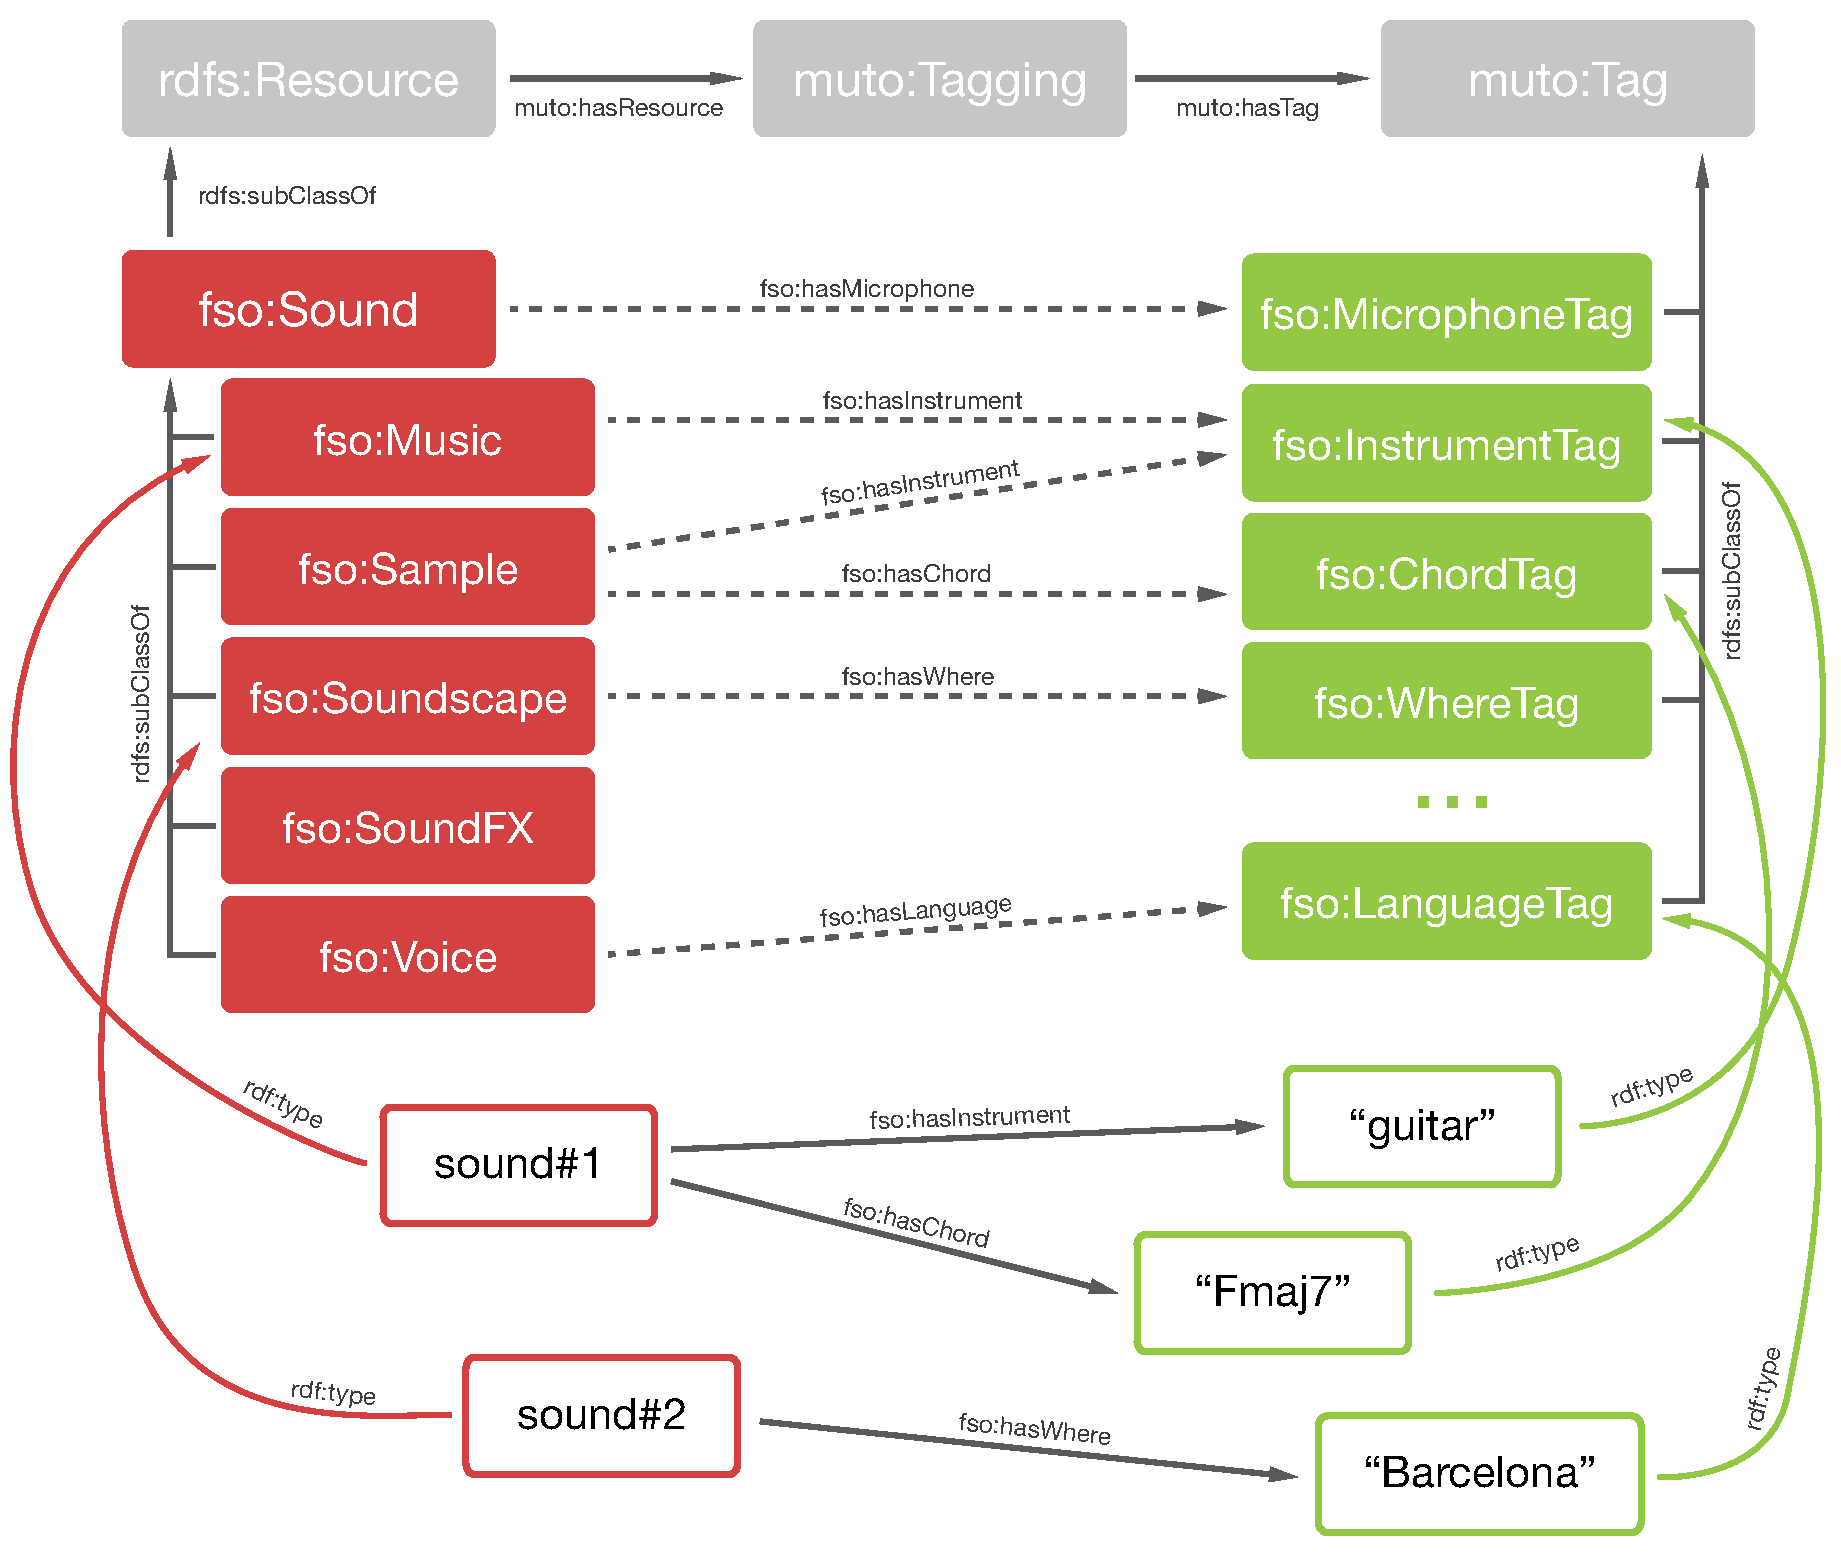
\includegraphics[width=1.0\textwidth]{ch06_ontology/pics/diagram_ontology_model}
  \caption[Conceptual diagram of the extension of the MUTO ontology]{Conceptual diagram of the extension of the MUTO ontology that drives the tag recommendation system. Solid boxes represent the classes of the ontology, while arrows indicate object properties. Dashed arrows represent the definitions of the object properties that relate audio categories with tag categories. The boxes at the bottom exemplify tag and resource instances. For the sake of clarity, only a small subset of \texttt{muto:Tag} subclasses are displayed in this figure. A complete list can be found in Table~\ref{tab:ontology_tag_categories}.}
  \label{fig:ontology_concept}
\end{figure}


Following the same idea of tag categories, we also extend the MUTO ontology by incorporating \atag{rdfs:Resource} subclasses that allow the grouping of resources into a number of audio categories (left side of Fig.~\ref{fig:ontology_concept}). 
%In the specific use case of our tag recommendation system, and given that we recommend tags for sounds, 
We define a generic \atag{fso:Sound} subclass for \atag{rdfs:Resource}, and five subclasses for the \atag{fso:Sound} class which correspond to the audio classes that we have already defined in our previous version of the tag recommendation system (Sec~\ref{class:sec:classification_system}). 
As it can be seen in Fig.~\ref{fig:ontology_concept}, the five subclasses of \atag{fso:Sound} are named in accordance with their corresponding audio class names.%\footnote{
%\texttt{fso:SoundFX} for \textsc{SoundFX}, 
%\texttt{fso:Soundscape} for \textsc{Soundscape}, 
%\texttt{fso:Sample} for \textsc{Sample}, 
%\texttt{fso:Music} for \textsc{Music} and 
%\texttt{fso:Voice} for \textsc{Voice}.}.

Finally, we also extend the tagging ontology by defining a number semantic relations in the form of object properties.
The purpose of these object properties is to represent relations between tag and resource instances (dashed lines in Fig.~\ref{fig:ontology_concept}).
Every included object property defines, as its range, a particular \atag{muto:Tag} subclass, and as its domain, at least one of the \atag{rdfs:Resource} subclasses. Therefore, we define as many object properties as tag categories. These object properties are named according to their ranged tag category. 
For example, the property \atag{fso:hasInstrument} ranges instances of \atag{fso:InstrumentTag}, and its domain includes instances of \atag{fso:Sample} and \atag{fso:Music} audio categories.
Therefore, \atag{fso:hasInstrument} can relate sounds belonging to either the \atag{fso:Sample} or \atag{fso:Music} classes, with tag instances of the type \atag{fso:Ins\-tru\-ment\-Tag}.
By inspecting the domains and ranges of these object properties, our ontology can determine which tag categories are relevant when describing a resource of a given audio category. 
For instance, and following the previous example, the ontology can determine that \atag{fso:InstrumentTag} tags, are relevant when annotating sounds of the \atag{fso:Music} or \atag{fso:Sample} audio categories, but that are not so relevant when annotating sounds of other categories such as \atag{fso:Soundscape}.
Object properties can be defined with multiple domains, meaning that a particular tag category can be considered relevant to more than one audio category.
In Table~\ref{tab:ontology_tag_categories} we show, for every tag category, its corresponding object property range, name and domain.

\begin{sidewaystable}
\ra{1.1}
\tiny
\begin{center}
\footnotesize
\begin{tabular}{@{}p{3.4cm}lp{4.6cm}l@{}}
\toprule
\textbf{Tag category/Object property range} & \textbf{Object property name} & \textbf{Object property domain} & \textbf{Information facet description} \\ 
\midrule 
\texttt{fso:ActionTag} & \texttt{fso:hasAction} & \texttt{fso:SoundFX}, \texttt{fso:Soundscape} & Physical activities captured in the recording \\
\texttt{fso:AgeTag} & \texttt{fso:hasAge} & \texttt{fso:Voice} & Age of the speaker or speakers \\
\texttt{fso:ArticulationTag} & \texttt{fso:hasArticulation} & \texttt{fso:Music}, \texttt{fso:Sample} & Performance or playing technique \\
\texttt{fso:ChordTag} & \texttt{fso:hasChord} & \texttt{fso:Music} & Music chords present in the recording \\
\texttt{fso:DynamicsTag} & \texttt{fso:hasDynamics} & \texttt{fso:Music}, \texttt{fso:Sample} & General loudness characteristics \\
\texttt{fso:EnvelopeTag} & \texttt{fso:hasEnvelope} & \texttt{fso:Sample} & Envelope of a sound at the note level \\
\texttt{fso:GearTag} & \texttt{fso:hasGear} & \texttt{fso:Sound} & Gear used to generate the sound \\
\texttt{fso:GenderTag} & \texttt{fso:hasGender} & \texttt{fso:Voice} & Gender of the speaker or speakers \\
\texttt{fso:GenreTag} & \texttt{fso:hasGenre} & \texttt{fso:Music}, \texttt{fso:Sample} & Music genre \\
\texttt{fso:InstrumentTag} & \texttt{fso:hasInstrument} & \texttt{fso:Music}, \texttt{fso:Sample} & Instrument names, brands or types \\
\texttt{fso:KeyTag} & \texttt{fso:hasKey} & \texttt{fso:Music} &  Music tonality of the recording  \\
\texttt{fso:LanguageTag} & \texttt{fso:hasLanguage} & \texttt{fso:Voice} & Languages present in the sound \\
\texttt{fso:MaterialTag} & \texttt{fso:hasMaterial} & \texttt{fso:SoundFX} & Material of sound sources present in the recording \\
\texttt{fso:MeterTag} & \texttt{fso:hasMeter} & \texttt{fso:Music} &  Music time signature information \\
\texttt{fso:MicrophoneTag} & \texttt{fso:hasMicrophone} & \texttt{fso:Sound} & Microphone names, brands and types \\
\texttt{fso:MoodTag} & \texttt{fso:hasMood} & \texttt{fso:Sound} & Moods and emotions conveyed by the sound \\
\texttt{fso:NoteTag} & \texttt{fso:hasNote} & \texttt{fso:Sample} & Music note present in the recording \\
\texttt{fso:OnomatopeiaTag} & \texttt{fso:hasOnomatopeia} & \texttt{fso:SoundFX} & Phonetic imitations of the sound \\
\texttt{fso:ProcessingTag} & \texttt{fso:hasProcessing} & \texttt{fso:Sound} & Techniques used to process the recording \\
\texttt{fso:RecordingTag} & \texttt{fso:hasRecording} & \texttt{fso:Sound} & Recording techniques used to produce the sound \\
\texttt{fso:SoftwareTag} & \texttt{fso:hasSoftware} & \texttt{fso:Sound} & Software names, brands or types \\
\texttt{fso:TempoTag} & \texttt{fso:hasTempo} & \texttt{fso:Music} & Tempo information \\
\texttt{fso:TypeTag} & \texttt{fso:hasType} & \texttt{fso:Sound} & Generic classification of a sound \\
\texttt{fso:WhatTag} & \texttt{fso:hasWhat} & \texttt{fso:SoundFX}, \texttt{fso:Soundscape} & Sound sources present in the recording \\
\texttt{fso:WhenTag} & \texttt{fso:hasWhen} & \texttt{fso:Soundscape} & Indication of the moment when the sound was recorded  \\
\texttt{fso:WhereTag} & \texttt{fso:hasWhere} & \texttt{fso:Soundscape} & Indication of the place where the sound was recorded \\
\bottomrule
\end{tabular}
\caption[Tag categories defined in the proposed ontology and their corresponding object properties]{Tag categories defined in the proposed ontology and their corresponding object properties.}
\label{tab:ontology_tag_categories}
\end{center}
\end{sidewaystable}

Using this ontology, it is possible to structure the information embedded in a folksonomy, and also to incorporate some meaningful semantic relations that will be used by our tag recommendation system. 
The ontology is specifically designed to fit the requirements of our use case, but it could be further extended to be capable of representing more classes of resources, tags and other semantic relations.
In fact, because the tag categories we define are of type \atag{muto:Tag}, and \atag{muto:Tag} inherits from SKOS\footnote{SKOS: Simple Knowledge Organisation System ontology. \url{http://www.w3.org/TR/skos-reference}.} class \atag{skos:Concept}, semantic relations between tag instances to represent, for example, synonymy and polysemy, could be easily included~\citep{Echarte2007,Lohmann2011}. An ontology-based tag recommendation system could then take advantage of these relations to refine tag suggestions. Furthermore, semantic relations between resources could also be defined by making resource subclasses inherit from \atag{skos:Concept}. 
However, the exploration of these possibilities is out of the scope of the work presented in this chapter.
Instead, we here show a simple approach in which tag recommendation can be driven by a domain-specific ontology.


\subsection{Ontology population}
\label{sec:ontology:population}

So far we have introduced the definition of the ontology that we use to drive our tag recommendation system.
We have seen that in using this ontology we are able to determine a number of tag categories that are considered relevant for a given audio category.
Using this information, the recommendation system could guide the annotation process by suggesting potentially relevant information facets to users.
However, our tag recommendation system also relies on the ontology for displaying the suggested tags grouped into tag categories.
At this point, the defined ontology does not yet contain any knowledge about the categorisation of particular tags into tag categories. Hence, it can not be used to meet the latter requirement. 
To overcome that limitation, we populate the ontology with a number of tag instances for the different tag categories.
In this way, and only for the tag instances that we populate, the ontology is able to tell to which tag category these belong, and the recommendation system can group them accordingly.

The population of the ontology was performed manually, and in parallel with the definition of the different tag categories of the ontology.
For the first stage, we selected the 500 most used tags in the folksonomy of Freesound, and built an interface in which we were presented with these tags one by one.
The interface allowed us to classify every tag into an existing tag category, or to create a new tag category if no existing categories fitted the tag at hand.
We started the process with no predefined tag categories.
The consideration of whether a given tag needed a new tag category or not is highly subjective. In general, the goal was to generate broad tag categories that could be easily understood by users in Freesound. We put a special emphasis on tags describing musical properties. Hence, some narrower tag categories were created for this domain (see below).  
After classifying all tags, we obtained a number of tag categories representative of the 500 most used tags in Freesound, and a number of tags classified under each category.
For the second stage, we manually reorganised some of these categories (combining or splitting them into new categories), and also added other categories that we considered were relevant and missing from the resulting list. 
Then, we were presented again with the 500 most used tags in Freesound, and classified them into the refined set of categories. 
Because of the ambiguity and unclear meaning of some tags, their classification into tag categories was not a straightforward task.
Furthermore, this problem was accentuated because tags were presented one by one and outside of the context of the sounds they were originally assigned to.
In some cases, tags were classified to more than one tag category. For example, the tag \atag{piano} can be considered as a tag describing the dynamics of a music recording (\atag{fso:DynamicsTag}), or as a tag describing the name of an instrument (\atag{fso:InstrumentTag}). Tags whose meaning was not clear or did not fit any of the refined tag categories were discarded.

As a result of the whole process, we obtained the set of 26 tag categories shown above in Table~\ref{tab:ontology_tag_categories}, and 413 of the 500 most used tags in Freesound classified into these categories. 
For each of the 413 tags, we populated the ontology with a tag instance of the corresponding tag category.
Therefore, after the population process, the ontology includes knowledge about the tag category (or categories) to which each one of these 413 tags belongs.
Although 413 tags represents less than 1\% of the total number of distinct tags in Freesound, these tags appear in 86\% of sound annotations, and are present in 51\% of tag applications. Therefore, we can estimate that the populated ontology is able to tell the tag category of roughly one out of two tags introduced by users when annotating sounds.
% n classified tags = 413
% n total tags = 66023 (2 november 2014)
% n associations that contain one of 413 tags: 803277 (50,63% of total 1586413)
% % of sounds that have at least one of the 413 tags: 86,47%

We mentioned that some of the tag categories we defined are designed with a narrower scope than other categories.
In particular, we define a number of very specific tag categories that describe musical properties such as \atag{fso:ChordTag} or \atag{fso:TempoTag}.
These categories can not be widely populated following the process described above because, in general, there are only a few tags among the 500 most used tags in Freesound that fit into these categories. This partially happens because there is not a clear agreement in the folksnomy of Freesound on how to annotate this kind of information. For example, in annotating tempo information, it is very common for some users to employ a tag such as \atag{120bpm}, whereas other users indicate the same information with the pair of tags \{\atag{120}, \atag{bpm}\}, or with a compound tag \atag{120-bpm}.
For these particular tag categories, which we refer to as ``narrow tag categories'', we performed an extra step of population in which we manually produced a list of invented tags (not necessarily chosen from existing tags in the Freesound folksonomy) and added them to the ontology. Hence, for some of the defined tag categories, we created a list of ``post-populated tags''.
Details on the importance of post-populated tags and how are they treated differently in the tag recommendation process are given in Sec.~\ref{sec:ontology:tag_recommendation}.
Besides post-populating narrow tag categories, we applied the same strategy to the \atag{fso:TypeTag} category. 
As shown in Table~\ref{tab:ontology_tag_categories}, \atag{fso:TypeTag} tags are intended to classify sounds into general categories. During the population process we classified several tags into this category.
Because of their nature, we consider that \atag{fso:TypeTag} tags are particularly important in the annotation of sounds. Hence, for trying to reinforce the agreement in the tags used under this category (see below), we post-populated \atag{fso:TypeTag} with a hand-crafted list of tags. This list includes some of the tags obtained with the normal population process, and some others that were added to create a more complete and coherent list of generic sound type tags.
In Table~\ref{tab:ontology_tag_categories_most_popular_tags} we show, for every tag category, the tags that have been post-populated (if any), and up to the 10th most used tags coming from the normal population process.

\begin{table}
\ra{1.2}
\begin{center}
\footnotesize
\begin{tabular}{@{}lp{10cm}@{}}
\toprule
\textbf{Tag category} & \textbf{Post-populated and normally-populated tags}  \\ 
\midrule 
\texttt{fso:ActionTag} & click, announcement, close, open, walking, drop, squeak, talking, crash, singing \\
\texttt{fso:AgeTag} & woman, girl, child, baby, children, boy, kids \\
\texttt{fso:ArticulationTag} & \textbf{vibrato}, \textbf{tenuto}, \textbf{staccato}, \textbf{legato}, \textbf{extended}, non-vibrato, extended, vibrato \\
\texttt{fso:ChordTag} & \textbf{A}, \textbf{C7}, \textbf{Fmaj7}, \textbf{Am9}, \textbf{Em}, \textbf{Gm7}, \textbf{Asus4}, \textbf{FSharp}, \textbf{DSharp7}, \textbf{FSharpm}, \textbf{Bb}, \textbf{Eb7}, \textbf{G/A} \\
\texttt{fso:DynamicsTag} & \textbf{pianissimo}, \textbf{piano}, \textbf{mezzo-piano}, \textbf{mezzo-forte}, \textbf{forte}, \textbf{fortissimo}, \textbf{midi-velocity-30}, \textbf{midi-velocity-64}, \textbf{midi-velocity-120}, piano, mezzoforte \\
\texttt{fso:EnvelopeTag} & \textbf{slow-attack}, \textbf{fast-attack}, \textbf{medium-attack}, \textbf{slow-release}, \textbf{fast-release}, \textbf{medium-release} \\
\texttt{fso:GearTag} & computer, tape, vinyl, zoom-h2n, zoom, roland, korg, waldorf, virus, atari \\
\texttt{fso:GenderTag} & male, female, woman, girl, man \\
\texttt{fso:GenreTag} & ambient, electronic, metal, electro, industrial, techno, house, trance, dance, dubstep \\
\texttt{fso:InstrumentTag} & drum, synth, electronic, percussion, bass, snare, guitar, kick, acoustic, digital \\
\texttt{fso:KeyTag} & \textbf{A}, \textbf{Cmaj}, \textbf{Emin}, \textbf{FSharpmin} \\
\texttt{fso:LanguageTag} & english, american, spanish, portuguese, accent \\
\texttt{fso:MaterialTag} & water, metal, wood, metallic, glass, plastic, paper, air, gas, steel \\
\texttt{fso:MeterTag} & \textbf{4-4}, \textbf{3-4}, \textbf{6-8}, \textbf{9-8} \\
\texttt{fso:MicrophoneTag} & neumann \\ %\textbf{sm58}, \textbf{rode}, \textbf{condenser}, \textbf{shotgun}, neumann \\
\texttt{fso:MoodTag} & horror, scary, funny, suspense, fun, dream, dramatic, tension \\
\texttt{fso:NoteTag} & \textbf{A}, \textbf{CSharp}, \textbf{Gb}, \textbf{A4}, \textbf{E3}, \textbf{FSharp4}, \textbf{Eb5}, \textbf{midi-note-35}, \textbf{midi-note-40}, \textbf{midi-note-64}, \textbf{midi-note-80}, \textbf{midi-note-127} \\
\texttt{fso:OnomatopeiaTag} & click, beep, rumble, ring, tone, bang, pop, buzz, bleep, rattle \\
\texttt{fso:ProcessingTag} & processed, reverb, distortion, echo, remix, unprocessed, filter, synthesis, delay, raw \\
\texttt{fso:RecordingTag} & stereo, binaural, mono, studio, xy \\
\texttt{fso:SoftwareTag} & reaktor, vst \\
\texttt{fso:TempoTag} & \textbf{120bpm}, \textbf{140bpm}, \textbf{60bpm}, 120bpm, 140bpm \\
\texttt{fso:TypeTag} & \textbf{field-recording}, \textbf{fx}, \textbf{soundscape}, \textbf{voice}, \textbf{multisample}, \textbf{single-note}, \textbf{percussive-hit}, \textbf{loop}, \textbf{music}, \textbf{chord}, \textbf{chord-progression}, \textbf{melody}, \textbf{rhythm}, field-recording, loop, 1-shot, drone, soundscape, beat, vocal, glitch, pad, hit \\
\texttt{fso:WhatTag} & noise, voice, water, birds, machine, wind, people, human, door, ambiance \\
\texttt{fso:WhenTag} & spring, night, summer, morning, winter \\
\texttt{fso:WhereTag} & space, nature, industrial, city, street, kitchen, field, station, forest, sea \\
\bottomrule
\end{tabular}
\caption[Examples of tags populated per tag category]{Examples of tags populated per tag category. Tags in bold correspond to those tags that were introduced in the post-population step (post-populated tags), while the other tags show up to the 10th most used tags coming from the normal population process (normally-populated tags).}
\label{tab:ontology_tag_categories_most_popular_tags}
\end{center}
\end{table}

%With the ontology defined and populated, we can perform queries such as: which are the relevant tag categories for a particular resource class, or which are the tags classified under a particular tag category, which is what is useful in our tag recommendation use case
%Note that in our particular use case we do not need to populate the ontology with sound instances, as the tag recommendation system only uses the ontology for grouping recommended tags into the defined tag categories and for determining relevant tag categories given an audio category (see below).


\subsection{Ontology-based tag recommendation}
\label{sec:ontology:tag_recommendation}

The ontology-based tag recommendation system we describe here is built upon the class-based tag recommendation described in Chapter~\ref{sec:class}.
In Fig.~\ref{ontology:fig:diagram}, we show a block diagram of the recommendation system and highlight the components that are added or modified with respect to the class-based recommendation system. 
We now summarise these additions. 
In the following sections, we describe in depth the new components of the ontology-based tag recommendation system as well as its implementation in terms of user interface.

\begin{figure}
  \centering
  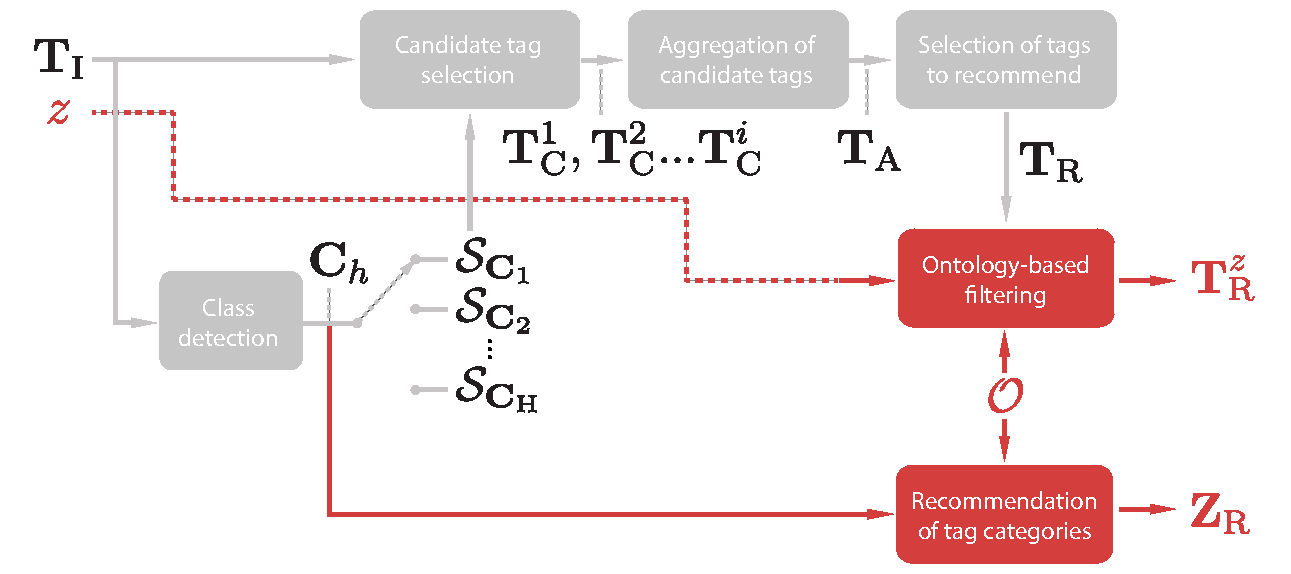
\includegraphics[width=1.0\columnwidth]{ch06_ontology/pics/recommendation_diagram.pdf}
  \caption[Block diagram of the ontology-based tag recommendation system]{Block diagram of the ontology-based tag recommendation system. Note that the ontology-based filtering step takes as input a tag category $\tagCategory$, and outputs a set of recommended tags $\recommendedTagsPerTagCategory$ which depends on $\tagCategory$. Also, further note that for generating $\recommendedTagsPerTagCategory$ and the list of recommended tag categories $\recommendedTagCategories$, the recommendation system relies on the ontology that we described in the previous sections (denoted here as $\ontology$). }
  \label{ontology:fig:diagram}
\end{figure}

\begin{itemize}
\item[i)] The set of recommended tags depends, as usual, on the input tags $\inputTags$ and on the tag-tag similarity matrix $\similarityMatrix_{\audioClass}$ of the audio class $\audioClass$ that is selected after the class detection step. However, in the ontology-based system, the recommendation also takes as input a tag category $\tagCategory$ ($\tagCategory \in \tagCategories$, where $\tagCategories$ is the set of defined tag categories) chosen by the user. %\footnote{To clarify notation in the following sections, we use the lowercase character $\tagCategory$ to refer to a tag category instead of a subscript notation like $\tagCategories_i$.}. 
This tag category is used to filter the output of the class-based system and produce the final set of $\recommendedTagsPerTagCategory$ recommended tags (``Ontology-based filtering'' step in Fig.~\ref{ontology:fig:diagram}).

\item[ii)] Besides outputting a list of recommended tags, the ontology-based tag recommendation system also produces a set of recommended tag categories $\recommendedTagCategories$ that depend on the audio class $\audioClass$ that is detected after the audio class detection step (``Recommendation of tag categories'' step in Fig.~\ref{ontology:fig:diagram}).
\end{itemize} 

%For generating both $\recommendedTagsPerTagCategory$ and $\recommendedTagCategories$, the recommendation system relies on the ontology that we already described (denoted here as $\ontology$). 
%In the following sections we describe more in depth the new steps of the ontology-based tag recommendation system as well as its implementation in terms of user interface.

\subsubsection{Ontology-based filtering of recommended tags}

Given a set of recommended tags $\recommendedTags$ (as produced by the class-based tag recommendation system) and an input tag category $\tagCategory$ chosen by the user, the ontology-based system performs the following operation to generate the final set of recommended tags $\recommendedTagsPerTagCategory$:
\[ \recommendedTagsPerTagCategory = \begin{cases} 
	\postPopulationForTagCategoryL \cup (\recommendedTags \cap \populationForTagCategoryL) & \text{if } |\recommendedTags| > 0 \\
	\postPopulationForTagCategoryL \cup \populationForTagCategoryL &\text{if } |\recommendedTags| = 0 \\
\end{cases}\text{,} \]
where $\populationForTagCategoryL$ is the set of normally-populated tags for the tag category $\tagCategory$, and $\postPopulationForTagCategoryL$ is the set of post-populated tags for $\tagCategory$. 
As it can be observed, if the first steps of the recommendation system (i.e.,~Candidate tag selection, Aggregation of candidate tags and Selection of tags to recommend) are able to generate a set of recommended tags $\recommendedTags$, the system filters that set $\recommendedTags$ by discarding all the tags not populated under the tag category $\tagCategory$. Then, the post-populated tags for the tag category (if any) are added on to the remaining tags in $\recommendedTags$ (duplicates are removed).
On the contrary, if $\recommendedTags$ can not be produced (typically because there are no input tags), the system recommends the union of the post-populated tags (if any) and the normally-populated tags for the corresponding tag category. In this case, normally-populated tags are sorted according to their global frequency of occurrence in the folksonomy of Freesound.

Note that for a given tag category, if there exist post-populated tags in the ontology, these are always recommended in the first place.
Therefore, post-populated tags always take a prominent position in the recommendation. With the exception of the tag category \atag{fso:TypeTag}, only narrow tag categories are post-populated (Sec.~\ref{sec:ontology:population}). The goal of this design choice is that the tags that are post-populated serve more as an example to users that as an actual recommendation. 
For instance, given the tag category \atag{fso:ChordTag}, the tags which are post-populated provide an idea of how to annotate chords (Table~\ref{tab:ontology_tag_categories_most_popular_tags}). Post-population of \atag{fso:ChordTag} includes tags such as \atag{Fmaj7} or \atag{Am9}. These particular chords probably do not suit most of the sounds for which they are recommended, but serve as an example of the syntax that users should follow when introducing chords. Thus, the post-population of tag categories is designed as a way to provide various examples rather than actual recommendations.
This concept also applies, to some extent, to the normally-populated tags that are recommended when $\recommendedTags$ is not generated. In that case, tags serve mostly as an example of what kind of information should be introduced in each tag category.
However, the post-population of the tag category \atag{fso:TypeTag} is performed to promote the usage of a particular set of predefined tags that categorise sounds into rather broad categories (Table~\ref{tab:ontology_tag_categories_most_popular_tags}). By having an extra control over the recommended tags for the \atag{fso:TypeTag} category, we expect that users will annotate the type of their sounds with a more unified vocabulary, using at least one of the tags that we recommend.

Furthermore, note also that the ontology-based tag recommendation system only recommends tags that are populated in the ontology $\ontology$. 
Thus, considering that our ontology is populated with a total of 413 unique tags, the recommendation system only recommends tags from that vocabulary of 413 tags. To overcome that limitation, a more comprehensive population of the ontology should be performed (see the discussion in Sec.~\ref{sec:ontology:conclusion}).


\subsubsection{Recommendation of tag categories}

An extra functionality for the ontology-based tag recommendation system is the suggestion of a set of potentially relevant tag categories $\recommendedTagCategories$ given a set of input tags $\inputTags$. 
This functionality is based on the audio class detection step introduced in the class-based tag recommendation system. 
Given a set of input tags, the classifier is able to predict to which audio class $\audioClass$ a sound belongs to (Sec.~\ref{class:sec:classification_system}).
In the ontology-based tag recommendation system, the predicted audio class $\audioClass$ is directly mapped to the corresponding audio category defined in the ontology (Sec.~\ref{sec:ontology:design}). Then, by considering the range of the object properties in $\ontology$ whose domain matches the predicted audio category, the system is able to generate a list of potentially relevant tag categories $\recommendedTagCategories$ (see below for an example). 

Note that some object properties have as its domain the generic audio class \atag{fso:Sound} (Table~\ref{tab:ontology_tag_categories}). By inheritance, any instance of the audio categories in the lower level of the hierarchy is also an instance of the class \atag{fso:Sound}. Therefore, these object properties are also considered and their corresponding tag categories are recommended. In fact, tag categories whose object property domain is the audio category \atag{fso:Sound} are always recommended.
For example, given a set of input tags whose detected audio category is \atag{fso:Voice}, $\recommendedTagCategories$ will include all tag categories related with \atag{fso:Sound} (e.g.,~\atag{fso:MicrophoneTag}, \atag{fso:TypeTag}, \atag{fso:ProcessingTag}, etc.), as well as all tag categories directly related with \atag{fso:Voice} (\atag{fso:LanguageTag}, \atag{fso:AgeTag} and \atag{fso:GenderTag}).
Those tag categories more related in first place with the detected audio category (i.e.,~not by inheritance), are positioned first in the list of recommended categories. We only make an exception with \atag{fso:TypeTag}, which is always placed in the first position to promote its usage.


\subsubsection{User interface of the annotation system}

The changes introduced in the ontology-based tag recommendation system with respect to the previous class-based system have important implications on the interface for annotating sounds. In Fig.~\ref{ontology:fig:interface}, we show three screenshots of that user interface.
As it can be observed, in an initial stage, the interface provides an input box in which users can start typing tags, and shows the list of all tag categories defined in the ontology (Fig.~\ref{ontology:fig:interface}a).
As soon as users type the first tag in the input box, the tag recommendation system can estimate an audio class $\audioClass$, and provide a recommendation of tag categories $\recommendedTagCategories$. When this happens, the list of tag categories is updated and divided into two parts. The top part lists tag categories in $\recommendedTagCategories$, and bottom part shows the rest of tag categories (Fig.~\ref{ontology:fig:interface}b).

\begin{figure}
  \centering
  \subbottom[]{
    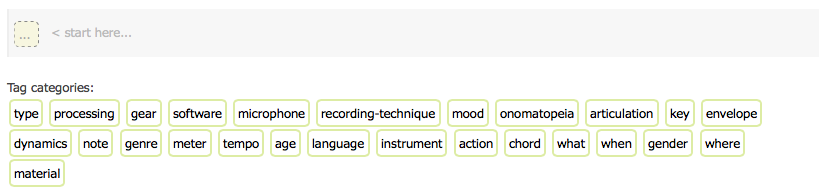
\includegraphics[width=0.87\columnwidth]{ch06_ontology/pics/interface_screenshot_a}}
  \subbottom[]{
    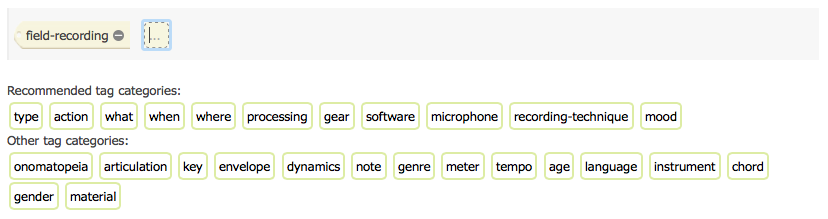
\includegraphics[width=0.87\columnwidth]{ch06_ontology/pics/interface_screenshot_d}}
  \subbottom[]{
    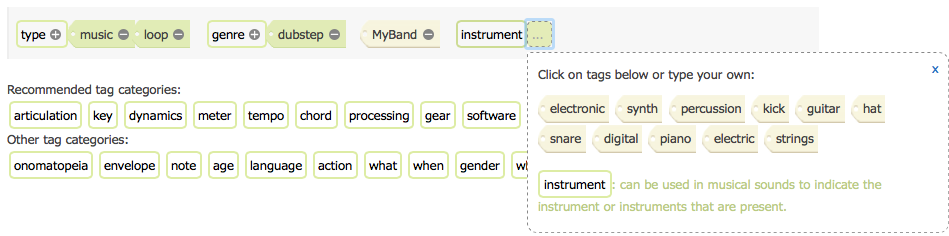
\includegraphics[width=1.0\columnwidth]{ch06_ontology/pics/interface_screenshot_c}}
  \centering
  \caption[Screenshots of the sound annotation interface]{Screenshots of the sound annotation interface using the ontology-based tag recommendation system. 
  Screenshot (a) shows the initial state of the interface, with no input tags introduced. 
  Screenshot (b) shows the interface with a single input tag \texttt{field-recording}.
  Screenshot (c) shows the state of the interface with the input tags $\inputTags=$\{\texttt{music}, \texttt{loop}, \texttt{dubstep}, \texttt{MyBand}\}, and showing tag recommendations for the tag category \texttt{fso:InstrumentTag}. In the latter example, the user has assigned the tags \texttt{music} and \texttt{loop} to the tag category \texttt{fso:TypeTag}, and the tag \texttt{dubstep} to the tag category \texttt{fso:GenreTag}. Notice that the tag \texttt{MyBand} is introduced with no assigned tag category.}
  \label{ontology:fig:interface}
\end{figure}

Users can introduce tags under the tag categories of the ontology by clicking on the tag category names displayed in the interface. When this happens, the tag category name is appended to the input box, and a pop-over appears which includes the recommended tags $\recommendedTagsPerTagCategory$ (Fig.~\ref{ontology:fig:interface}c). 
Similarly to the tag recommendation systems described in previous chapters, recommended tags are sorted according to the scores assigned during the aggregation step of the recommendation process (Sec.~\ref{sec:gen:step_2_aggregation}), but here we only show a maximum of 20 recommended tags.
Users can either choose to add one of the recommended tags or type their own. In either case, the introduced tag is assigned to the selected tag category as an attribute-tag (Sec~\ref{sec:ontology:introduction}).
Note that the vocabulary of tags that can be added under a tag category is not restricted. Hence, users can create new tags and assign them to any tag category.
Note also that multiple tags can be assigned to a single tag category.

Users are not forced to use any of the recommended tag categories, nor forced to use attribute-tags or click on recommended tags. In fact, users are not presented with any recommended tags until they click on one of the tag category names. In this way, the interface guides the annotation process by suggesting information facets and then providing tag recommendations for every information facet on demand, while at the same time it maintains the flexibility of previous tagging systems and allows users to continue tagging in their preferred way (i.e.,~without using attribute-tags).





\section{Evaluation}
\label{sec:ontology:evaluation_method}
% no quantitative definitions of tagging quality, definicio de qualitat de "On Incentive Based Tagging" Xuan S. 2013. the problem is that they refer to broad folksonomies (stability of tags) \cite{Yang2013a}

Here we describe the process we followed to evaluate whether the ontology-based tag recommendation system can better help users to generate comprehensive, coherent, and semantically meaningful resource annotations (when compared to the previous class-based recommendation system of Chapter~\ref{sec:class}).
For that purpose, we designed an online experiment in which participants have to tag a number of sounds from Freesound either using the ontology-based tag recommendation system or the class-based recommendation system. We analyse the logs collected during the experiment and compare both systems by computing a number of metrics.
To complement these results, we also perform a second experiment in which the ontology-based tag recommendation system is deployed in Freesound, and collect logs from real-world usage of the recommendation system. These logs are also analysed, when possible, using the same methodology of the previous experiment.
In the following sections, we describe the experiments and the analysis metrics we use to evaluate our system.

\subsection{Description of online experiments}
\label{sec:ontology:description_of_online_experiments}

\subsubsection{First experiment}

The first experiment was carried out during a time period of 22 days from 7 July 2014 to 13 August 2014. 
The different parts of the experiment are the same as those we used in Chapter~\ref{sec:class} for comparing the class-based tag recommendation system with previous systems (see Sec.~\ref{class:sec:evaluation}). 
Participants were first presented with a page with the instructions of the experiment and corresponding instructions of the tagging interface.
Then, participants had to fill in a questionnaire to collect some basic user data and information about their experience in working with sound libraries, their experience using Freesound and their native language.
After completing the questionnaire, participants could start the sound annotation phase.
We manually selected a pool of 20 sounds from Freesound, equally distributed in the five audio categories introduced in Chapter~\ref{sec:class} (Table~\ref{tab:audio_classes}). 
For each participant in the experiment, we randomly selected 3 sounds per category that had to be tagged. Therefore, participants had to annotate a total of 15 sounds.
The tagging interface was assigned at random per participant. Half of the participants used the ontology-based tag recommendation interface, while the other half used the class-based tag recommendation interface. We will refer to the ontology-based tag recommendation interface as \textsc{Ont}, and to the class-based interface as \textsc{Cla} for short.
In contrast to the experiment described in Chapter~\ref{sec:class}, in this experiment sounds were presented to users along with their original textual descriptions from Freesound. This was added to provide more context to participants and facilitate the tagging task (see discussion in Sec.~\ref{class:sec:user_feedback}).
After annotating the 15 sounds, participants were asked to answer a brief questionnaire to qualitatively evaluate some aspects of the tagging interface. 
We asked to all participants if the tagging interface was easy to understand, and if the tag recommendations were useful. Furthermore, to participants using the \textsc{Ont} interface, we also asked if tag categories were useful, understandable, and if there was enough variety of tag categories. All questions had to be answered using a 5-point scale, ranging from ``strongly disagree'' to ``strongly agree''. Finally, users were given the option to write a comment and provide in this way any other feedback they considered relevant.

Among the 195 participants of the experiment, 109 of them actually completed it.
The percentage of participants that completed the experiment is very similar to that obtained in the online experiment described in Chapter~\ref{sec:class}.
On average, we collected 70 alternative taglines for each sound of the aforementioned pool of 20 sounds, half provided using the \textsc{Ont} interface and half provided using the \textsc{Cla} interface.

\subsubsection{Second experiment}

The second experiment was carried out in Freesound after deploying the on\-to\-lo\-gy-based tag recommendation system as an optional experimental tagging interface. 
During a period of one week from 18 August 2014 to 25 August 2014, Freesound users were given the option to describe their sounds using the ontology-based tagging interface, labelled as an ``experimental tagging interface'' (\textsc{Ont}). Otherwise, users could still use the default tagging interface implemented in Freesound which, at the time of the experiment, was the class-based tagging interface (\textsc{Cla}).
The data collected in this experiment came from the usage of both interfaces in a real-world situation.
Hence, and as opposed to the first experiment, the sounds to be tagged were those uploaded by the users themselves, and we had no control over them.
Because of that, in this experiment, we could not collect multiple taglines per sound. Therefore, some of the analysis metrics that we compute for the first experiment can not be computed for the second experiment. 

During the period of the experiment we collected tagging data for 276 sounds and provided by 91 different Freesound users. 
Almost 70\% of the users chose to use the \textsc{Ont} interface. 
However, not all collected data can actually be included in our analysis.
The reason is that the interface of Freesound allows the description of up to 10 sounds at once, meaning that the information we extract from a single annotation session can correspond to the description of multiple sounds. 
During this process, users may describe sounds in a non-sequential way, and therefore our analysis metrics would not be completely reliable for annotation sessions with multiple sounds. 
For this reason, we only consider the information coming from these annotation sessions in which only one sound was described. As a result, the data that we finally analyse from the second experiment includes tagging data for 135 sounds, provided by 73 different Freesound users. Such data is evenly distributed between the two interfaces (48\% using \textsc{Ont} interface and 52\% using \textsc{Cla} interface).


\subsection{Analysis metrics}
\label{sec:ontology:analysis_metrics}

To analyse the logs collected in the online experiments and compare \textsc{Ont} and \textsc{Cla} tagging interfaces, we define a number of metrics that we divide in three groups. First, we compute simple quantitative metrics to evaluate aspects such as the time participants spend annotating sounds, the length of the tagline  and the number of correctly predicted tags of a given tagline.
Then, we perform a more semantic-oriented analysis in which we look at aspects such as the most commonly used tags and tag categories, and define metrics to roughly quantify the comprehensiveness and coherence of annotations.
Finally, we analyse the qualitative feedback that participants provide through the questionnaire at the end of the first experiment.
%In the following sections we describe and formalise these analysis metrics.


\subsubsection{Quantitative metrics}

We analyse the collected data using some of the quantitative measures already introduced in Chapter~\ref{sec:impact}.
These metrics include the average tagline length ($\metricAverageTaglineLength$), the average tag application time ($\metricAverageTagApplicationTime$), and the average number of correctly predicted tags ($\metricPercentageOfCorrectlyPredictedTags$), formalised in equations~\ref{impact:eq:average_tagline_length} (Sec.~\ref{impact:sec:definition_of_metrics}),~\ref{impact:eq:averae_tag_application_time} (Sec.~\ref{impact:sec:definition_of_metrics}), and~\ref{class:eq:n_accepted_tags} (Sec.~\ref{class:sec:evaluation}), respectively.
In Eq.~\ref{impact:eq:average_tagline_length}, a parameter $n$ is defined to explicitly restrict the set of sounds that are considered for computing the measure on an upload-date basis. In this analysis, we skip this parameter and simply consider a generic set of resources $\resources$. 
Besides these measures, we also include the following two new metrics:

%\item \textit{Average tag application time}: We measure the average time required for assigning a tag to an audio clip, using the average tag application time ($\metricAverageTagApplicationTime$) metric that we defined in Sec.~\ref{impact:sec:methods_cost_of_annotation}, Eq.~\ref{impact:eq:averae_tag_application_time}.
\begin{itemize}
\item \textit{Average time per sound}: Similarly to the average tag application time (Eq.~\ref{impact:eq:averae_tag_application_time}), the average time per sound measures the time required to annotate a sound (i.e.,~to generate a tagline for a sound), averaged over the sounds described in a set of annotation sessions. 
In our analysis, every annotation session corresponds to the description of one sound. Hence, average time per sound can be written as
\begin{equation} \metricAverageTimePerAudioClip =  \frac{1}{|\annotationSessions|}\sum\limits_{\annotationSession \in \annotationSessions}{\durationOfAnnotationSession}, \label{ontology:eq:average_time_per_audio_clip} \end{equation}
where $\durationOfAnnotationSession$ is the duration of an annotation session $\annotationSession$ (in seconds), and $\annotationSessions$ is a set of annotation sessions.

%\item \textit{Average tagline length}: This metric measures the average number of tags assigned to audio clips. A definition for this metric is given in Sec.~\ref{impact:sec:methods_cost_of_annotation}, Eq.~\ref{impact:eq:average_tagline_length}. However, for the current analysis we skip the parameter $n$ of Eq.~\ref{impact:eq:average_tagline_length} and simply consider a generic set of resources $\resources$. Hence, the average tagline length is the average number of tags of $\resources$.
%We already defined this metric in Sec.~\ref{impact:sec:methods_cost_of_annotation}, Eq.~\ref{impact:eq:average_tagline_length}. However, the definition in Eq.~\ref{impact:eq:average_tagline_length} includes the variable $n$ that is used to represent a particular period of time of the analysis. Here, we use a more generic definition such that
%\begin{equation} \metricAverageTaglineLength_\resources =  \frac{1}{|\resources|}\sum\limits_{\resource\in \resources}{|\tagApplicationsPerResourceR|}, \label{impact:eq:average_tagline_length} \end{equation}
%where $\tagApplicationsPerResourceR$ is the set of tag applications involving a resource $\resource$, and $\resources$ is a set of audio clips.

%\item \textit{Average number of correctly predicted tags}: This metric measures the average number of tags from an audio clip that were suggested by the recommendation system during the annotation process of that clip. The average number of correctly predicted tags ($\metricPercentageOfCorrectlyPredictedTags$) is formally defined in Sec.~\ref{impact:sec:methods_cost_of_annotation}, Eq.~\ref{impact:eq:percentage_of_correctly_predicted_tags}. Again, for the current analysis we skip the parameter $n$ of Eq.~\ref{impact:eq:percentage_of_correctly_predicted_tags} and simply consider a generic set of resources $\resources$.

\item \textit{Average percentage of attribute-tags}: We measure the percentage of attri\-bute-tags found in a tagline (i.e.,~the number of tags in a tagline that are introduced with a tag category), and average it over a set of resources. Hence, the average percentage of attribute tags can be formalised as
\begin{equation} \metricPercentageOfAttributeTags = \frac{100}{|\resources|}\sum\limits_{\resource\in \resources}{\frac{| \setOfAttributeTags^{r} |}{ | \tagsOfSoundR | }}, \label{ontology:eq:percentage_of_attribute_tags} \end{equation}
where $\setOfAttributeTags^{r}$ is the set of attribute tags of a resource $\resource$ (i.e.,~tags with category), $\tagsOfSoundR$ is the set of all tags of a resource $\resource$, and $\resources$ is a set of sounds.
This metric can be only computed for data collected from the \textsc{Ont} tagging interface, as attribute-tags are a particular feature of that interface.
\end{itemize}


\subsubsection{Semantic analysis}

The second part of the analysis we perform is focused on semantic aspects of the annotations.
On the one hand, we look at a list of the most common correctly predicted tags for both interfaces (i.e.,~those tags recommended by the system which are most commonly added to the taglines). In this way, we can have an idea of what kind of tags seem to be more useful as recommendations.
On the other hand, we examine which are the most commonly used tag categories in data collected using the \textsc{Ont} interface. From all tags used in every category, we also compute the percentage of them that were actually recommended by the recommendation system (i.e.,~correctly predicted). In this way, we can have an idea of which are the most useful tag categories and about how effective the recommendation system is in every category.
Also, in order to have an indication of whether the tag categories included in the ontology were enough for annotating the sounds, we have a look at those tags that were introduced without category (non-attribute-tags), and see if these could have been categorised under the existing categories or some of them might require the inclusion of new ones.
The latter analyses are also only applicable to the \textsc{Ont} tagging interface.

Besides looking at the previous aspects, we further define two analysis metrics which provide an estimation of the comprehensiveness and coherence of sound annotations generated with both interfaces. These two metrics are based on the analysis of the alternative taglines that we collected for every sound in the first experiment: %Hence, these can not be applied to the data collected from the second experiment. What follows is the definition of these metrics.

\begin{itemize}
\item \textit{Annotation comprehensiveness}: %The purpose of annotation comprehensiveness is to give an orientative measure of how comprehensive a tagline for a particular resource is. 
Comprehensiveness is measured in terms of the number of distinct information facets that are covered in a tagline. In essence, the more information facets are annotated, the more comprehensive the tagline is considered to be.
For each sound annotated in the first experiment, we collected an average of 70 alternative taglines, approximately half of them generated with the \textsc{Ont} interface and half with the \textsc{Cla} interface (Sec.~\ref{sec:ontology:description_of_online_experiments}).
Considering all the alternative taglines for a given sound, we build an annotation ground truth for that sound, which is then used to evaluate how comprehensive individual taglines are. 

To construct the ground truth for a given sound, we aggregate the individual tags of all alternative taglines into a single set of tags, and manually group them into several information facets. The category of attribute-tags is removed, so that we only add the actual tag to that list. Then, to group the list of tags, we follow a similar process to that described for the definition and population of the tag categories in the ontology (Sec.~\ref{sec:ontology:population}). Given that, in this case, the grouping of tags is performed with the actual sound as a reference, tags can be grouped according to the kind of information they describe in the context of that particular sound. Hence, the process becomes simpler and less ambiguous.
As a result, we obtain a number of information facets with a set of tags classified into them. 
Given the ground truth and a tagline for a sound, the comprehensiveness of a tagline is computed by comparing the number of information facets covered by the tagline (i.e.,~the number of facets from the ground truth for which there is at least one tag in the tagline), with the total number of possible information facets defined in the ground truth.
Hence, given the intermediate function
\[ covered(\mathbf{X},\mathbf{Y}) = \begin{cases} 
	1 & \text{if } |\mathbf{X} \cap \mathbf{Y}| > 0 \\
	0 & \text{if } |\mathbf{X} \cap \mathbf{Y}| = 0 \\
\end{cases}\text{,}\]
annotation comprehensiveness is defined as
\begin{equation} \metricAnnotationComprehensiveness = \frac{1}{|\groundTruthForResourceR|}\sum\limits_{\tags_\text{IF} \in \groundTruthForResourceR}{covered(\tagsOfSoundR, \tags_\text{IF})}
\text{,} 
\label{ontology:eq:annotation_comprehensiveness} \end{equation}
where $\tagsOfSoundR$ is the tagline of a resource $\resource$, $\groundTruthForResourceR$ is the ground truth of a resource $\resource$, and $\tags_\text{IF}$ is a set of tags corresponding to one of the information facets defined in $\groundTruthForResourceR$.
Using this measure, we can estimate how comprehensive are, individually, each of the alternative taglines provided for every annotated sound. Then, we can compare the annotation comprehensiveness of \textsc{Ont} and \textsc{Cla} interfaces by averaging this measure over all the taglines generated with each interface.

\item \textit{(In)coherence in annotations}: To evaluate the coherence of a set of alternative taglines for a given sound we, in fact, define a measure of incoherence.
Incoherence is measured in terms of the variety of tags that are used to convey a unique semantic meaning (or audio property).
The more variety of tags is used to describe a particular property in a set of taglines for a given sound, the more incoherent these taglines are considered to be. 
For example, given an audio recording of a musical instrument playing a chord, a set of taglines that feature tags like \atag{DMaj}, \atag{D-major}, \atag{Dmajor} and \atag{DM} to indicate the chord, is more incoherent than another set of taglines in which the chord is always indicated with either \atag{DMaj} or \atag{Dmajor} (using fewer variations). In a sense, the incoherence in annotations reflects the agreement on how to annotate particular audio properties among the participants that generated the taglines.
Similarly to annotation comprehensiveness, we estimate the incoherence in annotations by building an annotation ground truth for each of the sounds annotated in the first experiment. Then, this ground truth is used to estimate the incoherence of the taglines of the corresponding sound.
Hence, incoherence in annotations can only be computed on data collected in the first experiment.

The annotation ground truth that we build for this measure is different to that built for annotation comprehensiveness.
Here, given a sound, we also aggregate the individual tags of all alternative taglines into a single set of tags, but instead of grouping them into rather broad information facets, we group together those tags that convey the same or very similar information.
For example, we group together tags like \{\atag{Funk}, \atag{funk}, \atag{funky}\}, which denote the same music genre, tags like \{\atag{distortion}, \atag{smooth-distortion}, \atag{distorted},\atag{overdrive}\}, which all describe a very similar audio processing effect, or tags like \{\atag{talking}, \atag{speak}, \atag{talk}, \atag{chatting}, \atag{speaking}\}, which refer to the same activity. Tags with no other equivalent (or very similar) tags are not considered in the ground truth.
As a result, the annotation ground truth for a sound consists of a list of sets of tags that are almost equivalent from a semantic point of view (i.e.,~a list of \emph{synsets}\footnote{To simplify explanations, we adopt the terminology used in WordNet~\citep{Miller1995}, which refers to a set of synonyms as a ``synset''. In our case, we use the term synset with a slightly broader meaning, as tags are not strictly grouped because of being synonyms, but because of featuring high semantic equivalence.}). 
Considering the ground truth for a sound and a set of alternative taglines, we iterate over its identified synsets and count how many of the tags in the synset are present in the set of taglines. Averaging that value over the different synsets, we obtain an indication of the incoherence in a set of taglines. %Note that the measure we compute is, in fact, a measure of ``incoherence'' in annotations, as the higher the result, the less coherent the taglines are considered to be. Nevertheless, 
The measure can be formalised as 
\begin{equation} \metricCoherenceInAnnotations = \frac{1}{|\groundTruthForResourceR|}\sum\limits_{\tags_\text{SY} \in \groundTruthForResourceR}{|\tagsOfSoundR_\text{TL} \cap \tags_\text{SY}| }
\text{,} 
\label{ontology:eq:choerence_in_annotations} \end{equation}
where $\tagsOfSoundR_\text{TL}$ is the union of all tags from a set of taglines of a resource $\resource$, $\groundTruthForResourceR$ is the annotation ground truth of a resource $\resource$, and $\tags_\text{SY}$ is a set of tags corresponding to one of the synsets defined in $\groundTruthForResourceR$.
Using this measure, we can estimate how incoherent a set of taglines is for a given sound. By computing this measure over sets of taglines collected with the \textsc{Ont} and \textsc{Cla} interfaces, we can compare them in terms of incoherence in resulting annotations.

\end{itemize}

\subsubsection{Qualitative feedback}
To analyse the qualitative feeback provided by users we compute the average over the responses of the different questions answered in the 5-point scale (see Sec.~\ref{sec:ontology:results_qualitative_feedback}), and relate these with the results of the quantitative and semantic analysis. 
Furthermore, we compare the responses of these questions which are common to participants using both interfaces.
Finally, we comment on the extra qualitative feeback that we collected in the form of textual comments.


\subsection{Analysis methodology}
\label{sec:ontology:analysis_methodology}

The analysis we perform is mainly centred on the data collected from the first experiment. This is because, as we have seen, the nature of the second experiment does not allow us to compute all the metrics listed above. Hence, the analysis of the data from the second experiment is used, whenever available, as a complement to the analysis of the first experiment. Nevertheless, with the exception of some metrics, we use the same methodology to analyse the data collected from both experiments. In general, we consider data generated with the \textsc{Ont} interface separated from data generated with the \textsc{Cla} interface, and then compare the results of the different metrics. Statistical significance is assessed using the Mann-Whitney U test with a significance level of 0.05~\citep{Corder2009}.
%test was previously cited as ~\citep{Mann1947}.

Before computing the analysis measures described above, we filter the collected data to remove potentially irrelevant or noisy logs.
The filter is applied at the sound level, meaning that we discard the information from individual sounds that do not pass the filter.
The first filter we compute operates on the duration of annotation sessions for sounds.
We discard annotation sessions based on the interquartile range of their duration.
Let $q_1$ be the first quartile and $q_3$ be the third quartile of the durations of annotation sessions, we discard sounds whose annotation session duration is outside the range $[q_1 - 3(q_3 - q_1), q_3 + 3(q_3 - q_1)]$. In practice, this means that we only consider data corresponding to sounds that were annotated in less than 260 seconds.
We apply a second filter in which we discard all sound annotation sessions in which there are no logged \emph{calls} to the tag recommendation system. In these sessions, no tag recommendations were provided to the user. This might happen because of different reasons (see below).
%We consider that annotation sessions that do not comply with both filters are not reliable for our analysis. 
%In some cases, we also report results that consider annotation sessions without applying that filter. We do that when it is useful to illustrate some particular aspects of our analysis.


After applying the filter to all collected annotation sessions of the first experiment, we see that 69\% pass the filter. 
Most of the annotation sessions comply with the timing restriction (97\%), but only 72\% feature at least one call to the recommendation system. 
Annotation sessions that do not pass the filter mostly correspond to sessions using the \textsc{Ont} interface.
%This is because only 42\% of sessions using the \textsc{Ont} interface feature at least one call to the recommendation system.%, whereas virtually all \textsc{Cla} sessions interface (99\%) feature at least one call.
This observation can be partially explained because, when using the \textsc{Ont} interface, tags are only recommended when users click on the tag categories (Sec.~\ref{sec:ontology:tag_recommendation}).
Conversely, when using the \textsc{Cla} interface, tags are automatically recommended when users start typing.
As a consequence, it can happen, particularly when using the \textsc{Ont} interface, that no tags are recommended at all.
We observe that only 42\% of annotation sessions using the \textsc{Ont} interface feature at least one call to the recommendation system.
Possible reasons for that could be that users do not properly understand how the interface works or that they do not think that tag categories are meaningful or necessary.
%This could be either because users do not properly understand how the interface works, because they do not think that tag categories are useful, or even because of technical problems causing errors in the interface.
Overall, the fact that less than half of the annotation sessions using the \textsc{Ont} interface pass both filters indicates that a lot of participants, for whatever reason, did not take advantage of the features of the interface as we expected. 
When applying the filter to the data from the second experiment, we observe practically the same percentages.
Therefore, one interesting aspect of the \textsc{Ont} interface that should be further investigated is why such a big percentage of users does not take advantage of recommendation functionalities as we expected (see discussion in Sec.~\ref{sec:ontology:conclusion}).


\section{Results}
\label{sec:ontology:results}

\subsection{Quantitative metrics}
\subsubsection{Average time per sound}

%EXP 1
%Statistical test (alpha=0.050000):
%	cur: avg:60.9222 std:41.3242 med:51.5000 - 784 values
%	ont: avg:108.5625 std:55.8287 med:95.0000 - 272 values
%	delta: 47.640306 test: 47992.000000 p_value 5.279e-42

%EXP 2
%Statistical test (alpha=0.050000):
%	cur: avg:155.6167 std:125.0467 med:121.0000 - 60 values
%	ont: avg:301.0625 std:188.6306 med:254.5000 - 32 values
%	delta: 145.445833 test: 500.000000 p_value 8.259e-05

The average time per sound $\metricAverageTimePerAudioClip$ reveals that sound annotations tend to require more time when using the \textsc{Ont} interface.
In particular, we observe a statistically significant average increase of 48 seconds ($\pvalue = 5.28\cdot 10^{-42}$). Fig.~\ref{fig:ontology:time_per_sound} shows the probability density function of the time per sound for both interfaces. The average time per sound is of 60 seconds for participants using the \textsc{Cla} interface, and of 109 seconds for participants using the \textsc{Ont} interface.
Similarly, when looking at real-world data from the second experiment, we also observe that users that choose the \textsc{Ont} interface spend more time annotating their sounds. In this case, the average time per sound of both interfaces is significantly higher than in the first experiment (156 seconds for \textsc{Cla} and 301 seconds for \textsc{Ont}), and so it is the difference between them (145 seconds, $\pvalue = 8.27\cdot 10^{-5}$).
This can be explained because, in the second experiment, users do not only have to annotate sounds, but also have to provide other information which is required by the Freesound uploading interface. This information includes a name for the sound, a textual description, a license and, optionally, geolocation and pack\footnote{In Freesound, sounds can be explicitly grouped in packs that users define.} information.
Furthermore, the increased difference between both interfaces observed in the second experiment can also be due to users experimenting with the interface to understand how it works. In the first experiment, before starting to annotate sounds, users were provided with instructions for the corresponding interface. Conversely, in Freesound, these instructions were not provided beforehand, and could only be accessed through a link that was provided during the annotation process.

\begin{figure}[t]
  \centering
  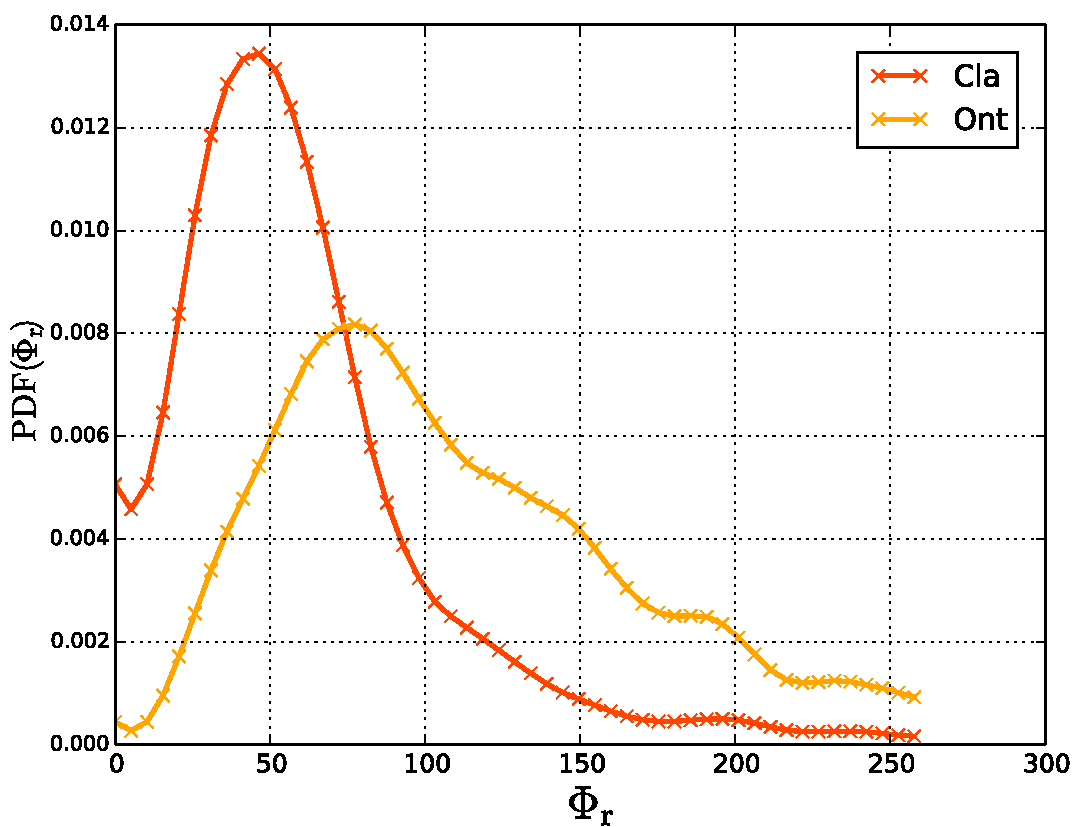
\includegraphics[width=\figSizeMidLarge]{ch06_ontology/pics/time_per_sound_pdf}
  \caption[Probability density function of the time per sound]{Probability density function of the time per sound $\metricAverageTimePerAudioClip$ with \textsc{Ont} and \textsc{Cla} interfaces. Curves are smoothed using a Hann window of 11 points.}
  \label{fig:ontology:time_per_sound}
\end{figure}

\subsubsection{Average tag application time}

% EXP 1
%Statistical test (alpha=0.050000):
%	cur: avg:11.0031 std:9.1202 med:8.7500 - 784 values
%	ont: avg:20.4508 std:17.4559 med:18.0000 - 272 values
%	delta: 9.447769 test: 48526.500000 p_value 2.82e-41

% EXP 2
%Statistical test (alpha=0.050000):
%	cur: avg:19.3058 std:23.4081 med:11.0682 - 60 values
%	ont: avg:47.0138 std:46.4678 med:33.3246 - 32 values
%	delta: 27.708056 test: 387.000000 p_value 1.344e-06

The average tag application time $\metricAverageTagApplicationTime$ features a very similar behaviour to that observed with $\metricAverageTimePerAudioClip$.
Participants of the first experiment need, on average, 11 seconds for assigning a tag using the \textsc{Cla} interface, and 20 seconds using the \textsc{Ont} interface. The increase of 9 seconds is statistically significant ($\pvalue = 2.82\cdot 10^{-41}$).
Similarly, in the second experiment, both the increase of the average tag application time is higher (28 seconds, $\pvalue = 1.34\cdot 10^{-6}$), and also the average times for both interfaces (19 seconds for \textsc{Cla} and 47 seconds for \textsc{Ont}).
Besides being in line with the previous measure, these results suggest that the extra time that users require for annotating sounds with the \textsc{Ont} interface is not because the generated taglines are longer, but because the assignment of each tag requires more time. 
%However, this aspect is better represented in the following metric.


\subsubsection{Average tagline length}

% EXP 1
%Statistical test (alpha=0.050000):
%	cur: avg:6.2398 std:2.9034 med:6.0000 - 784 values
%	ont: avg:6.6140 std:3.7790 med:6.0000 - 272 values
%	delta: 0.374175 test: 105296.500000 p_value 0.3789

% EXP 2
%Statistical test (alpha=0.050000):
%	cur: avg:12.0667 std:6.5799 med:11.0000 - 60 values
%	ont: avg:9.0938 std:5.7682 med:8.5000 - 32 values
%	delta: -2.972917 test: 720.000000 p_value 0.02447

The observations on the average tagline length that we can make by analysing the data from the first experiment confirm the previous suggestion that taglines do not tend to be longer for participants using the \textsc{Ont} interface. Although the average tagline length is slightly higher (6.61 tags for \textsc{Ont} interface and 6.24 tags for \textsc{Cla} interface), the difference is not statistically significant.
However, the results of the average tagline length computed for the second experiment are surprising. In this case, we observe that taglines using the \textsc{Cla} interface are in fact longer that those generated with the \textsc{Ont} interface (12.07 tags and 9.10 tags respectively, $\pvalue = 2.45\cdot 10^{-2}$).
The reason for this behaviour is not clear. One possible explanation is that with the usage of attribute-tags, sound annotations may appear to be more specific and complete while using fewer tags. Hence, users might feel that the description is good enough using fewer tags. In practice, the \textsc{Ont} interface merges tag categories and actual tags in the same space (see Fig.~\ref{ontology:fig:interface}), and this might cause the perception that the tagline is longer than it actually is.
%Another possible explanation could be the inexperience of users with the \textsc{Ont} interface.



\subsubsection{Average number of correctly predicted tags}

% EXP 1
%Statistical test (alpha=0.050000):
%	cur: avg:2.4834 std:2.1618 med:2.0000 - 784 values
%	ont: avg:2.5956 std:2.0629 med:2.0000 - 272 values
%	delta: 0.112170 test: 101629.500000 p_value 0.1215

% EXP 2
%Statistical test (alpha=0.050000):
%	cur: avg:3.3000 std:2.9569 med:3.0000 - 60 values
%	ont: avg:2.9688 std:2.4935 med:2.0000 - 32 values
%	delta: -0.331250 test: 915.000000 p_value 0.3563


The analysis of the average number of correctly predicted tags does not reveal a significant difference when comparing interfaces.
Sounds annotated with the \textsc{Cla} interface feature an average of 2.48 correctly predicted tags, which is very similar to that obtained in our previous evaluation of the \textsc{Cla} recommendation method (Chapter~\ref{sec:class}, Table \ref{tab:results_general_ub}), and of the impact of the tag recommendation system (Chapter~\ref{sec:impact}, Sec.~\ref{impact:sec:percentage_correcly_predicted_tags_results}).
Sounds annotated with the \textsc{Ont} interface feature a slightly higher average of 2.60 correctly predicted tags, but the difference is not statistically significant ($\pvalue = 1.22\cdot 10^{-1}$).
On the data collected for the second experiment, we again observe similar results with no statistically significant differences between interfaces (average of 3.30 and 2.97 correctly predicted tags for \textsc{Ont} and \textsc{Cla} interfaces, respectively, $\pvalue = 3.56\cdot 10^{-1}$).
What these results suggest is that the grouping of tags into tag categories and the recommendation of post-populated tags provided by the \textsc{Ont} interface does substantially not impact the number of tags from taglines that are correctly predicted by the recommendation system. 

Similarly to what we did in Chapter~\ref{sec:class}, we analysed if there is a correlation between the average number of correctly predicted tags and users' expertise and language (Sec.~\ref{class:sec:accepted_tags_results}). In particular, we consider the results from the first experiment and divide collected logs between groups of experienced and non-experienced participants, and native and non-native English speakers. Accordingly to what we describe in Sec.~\ref{class:sec:accepted_tags_results}, we observe here small increases in the number of correctly predicted tags for both expert and native speaker participants (in both interfaces). However, as opposed to the previous analyses, the differences in this case do not appear to be statistically significant.
Further research should be carried out in order to make stronger claims regarding that matter.
%Therefore, this result partially questions our previous specific findings regarding that matter and should be further researched. 


\subsubsection{Average percentage of attribute-tags}

% EXP 1
%Basic stats:
%	Percentage of tags with category: avg:0.7244 std:0.3521 med:1.0000 - 272 values
%41.30\% of sounds have at least one semantic tag (no filtering)

%Correlation with user experience
%Labels index:
%	1: Non experienced,ont
%	2: Experienced,ont
%General stats:
%	Non experienced,ont      0.6247 (0.4244) - 63 values
%	Experienced,ont          0.7545 (0.3212) - 209 values
%Statistical test data:
%-           1           2           
%1           -           3.855e-02   
%2           3.855e-02   -           

% EXP 2
% Basic stats:
%	Percentage of tags with category: avg:0.6359 std:0.3988 med:1.0000 - 32 values
%57.14\% of sounds have at least one semantic tag (no filtering)

Considering the taglines generated with the \textsc{Ont} interface for our first experiment, we observe that an average of 72\% of the tags are introduced under a tag category (i.e.,~are attribute-tags). In the second experiment, this percentage is slightly lower, at 65\%.
This means that a significant number of tags from taglines are contextualised in one of the defined tag categories of the ontology, and therefore their semantic value is effectively improved.
However, it is important to note that these percentages are achieved when considering filtered data as described in Sec.~\ref{sec:ontology:analysis_methodology}. This filter removes, among others, data from annotation sessions in which participants do not take advantage of the tagging interface as we expected. %Hence, the average percentage of attribute-tags is greatly affected by the filter. 
In Fig.~\ref{fig:ontology:percentage_of_attribute_tags}, we show the histogram of the number of attribute tags per tagline when considering unfiltered data for the first experiment. What we observe now is that more than half of the taglines (59\%) feature no attribute-tags, whereas other taglines tend to have between 1 and 7 attribute-tags. A similar observation can be made in the second experiment, with 43\% of taglines featuring no attribute-tags.
These results suggest that the tagging interface should better encourage the usage of attribute-tags.

\begin{figure}[t]
  \centering
  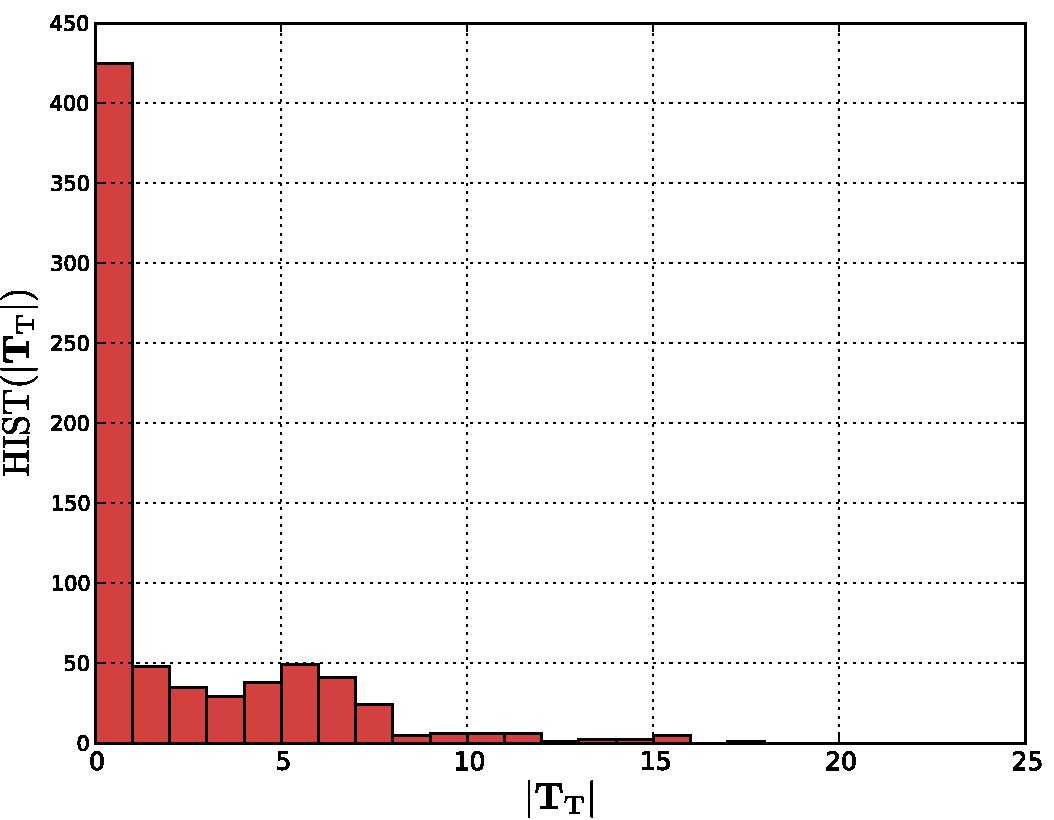
\includegraphics[width=\figSizeMidLarge]{ch06_ontology/pics/number_of_semantic_tags_histogram_no_filter}
  \caption[Histogram of the number of attribute-tags per tagline]{Histogram of the number of attribute-tags per tagline $|\setOfAttributeTags|$ in the first experiment (including unfiltered data).}
  \label{fig:ontology:percentage_of_attribute_tags}
\end{figure}

To complement these results, we analyse if there is a correlation between users' expertise and the percentage of attribute-tags. We observe that experienced users tend to include, on average, 13\% more attribute-tags than non-experienced users, that difference being statistically significant ($\pvalue = 3.86\cdot 10^{-2}$). This might be explained because experienced users better understand the advantages that attribute-tags provide in terms of description accurateness and further retrieval possibilities.


\subsection{Semantic analysis}

\subsubsection{Most common correctly predicted tags}

\begin{table}
\ra{1.2}
\begin{center}
\footnotesize
\begin{tabular}{@{}p{2cm}p{5cm}p{5cm}@{}}
\toprule
\textbf{Experiment} & \textsc{Ont} \textbf{interface} & \textsc{Cla} \textbf{interface} \\
\midrule
First & field-recording, voice, synth, condenser, single-note, fx, loop, soundscape, stereo, ambiance, 120bpm, electronic, percussive-hit, city, mezzo-forte, fast-attack, processed, mono, male, rhythm & field-recording, electronic, loop, synth, voice, people, rain, male, bell, child, weather, female, ring, nature, bells, vocal, beat, ambience, writing, city \\
%First & field-recording~(32), voice~(31), synth~(26), condenser~(23), single-note~(23), fx~(23), loop~(20), soundscape~(17), stereo~(17), ambiance~(15), 120bpm~(13), electronic~(12), percussive-hit~(11), city~(11), mezzo-forte~(11), fast-attack~(10), processed~(10), mono~(9), male~(9), rhythm~(8) & field-recording~(57), electronic~(46), loop~(39), synth~(35), voice~(32), people~(25), rain~(23), male~(22), bell~(22), child~(22), weather~(22), female~(21), ring~(21), nature~(21), bells~(21), vocal~(20), beat~(20), ambience~(19), writing~(19), city~(19) \\
Second & fx, soundscape, field-recording, talking, horror, condenser, stereo, male, english, voice, loop, summer, atmosphere, neumann, crowd, pop, distortion, suspense, female, violin & drums, drum, atmosphere, fx, ten, dance, house, ambiance, gloomy, deep, down, cavern, ambient, rave, chime, airplane, electronic, monster, sub, 0 \\
%Second & fx~(3), soundscape~(3), field-recording~(3), talking~(2), horror~(2), condenser~(2), stereo~(2), male~(2), english~(2), voice~(2), loop~(2), summer~(1), atmosphere~(1), neumann~(1), crowd~(1), pop~(1), distortion~(1), suspense~(1), female~(1), violin~(1) & drums~(2), drum~(2), atmosphere~(1), fx~(1), ten~(1), dance~(1), house~(1), ambiance~(1), gloomy~(1), deep~(1), down~(1), cavern~(1), ambient~(1), rave~(1), chime~(1), airplane~(1), electronic~(1), monster~(1), sub~(1), 0~(1) \\
\bottomrule
\end{tabular}
\caption[Most common correctly predicted tags]{First 20 most common correctly predicted tags for the first and second experiments and for \textsc{Ont} and \textsc{Cla} interfaces. 
%In parenthesis we indicate the total number of tag occurrences.
}
\label{tab:ontology_most_correctly_predicted_tags}
\end{center}
\end{table}

The most common correctly predicted tags for both experiments and interfaces are listed in Table~\ref{tab:ontology_most_correctly_predicted_tags}.
Looking at the tags of the first experiment, we observe that, regardless of the interface, an important number of tags have a semantic meaning that would belong to the \atag{fso:TypeTag} category (e.g.,~\atag{field-recording}, \atag{voice}, \atag{ambiance}). Other common tags belong to well defined musical concepts (e.g.,~\atag{loop}, \atag{synth}, \atag{electronic}, particularly in the \textsc{Ont} interface). Overall, both interfaces present similar (or very related) most common correctly predicted tags. In fact, 20\% of the first 50 most common correctly predicted tags in \textsc{Ont} and \text{Cla} interfaces are \emph{exactly} the same. 
This can be explained because the pool of sounds to annotate in the first experiment was limited to 20 sounds, and the concepts to annotate are determined by the sounds. 
However, of particular interest is the case of very specific tags such as \atag{120bpm}, \atag{mezzo-forte} and \atag{fast-attack}, which are included in the list of most common correctly predicted tags for the \textsc{Ont} interface. 
These tags are post-populated under the \atag{fso:TempoTag}, \atag{fso:DynamicsTag} and \atag{fso:EnvelopeTag} categories respectively (Table~\ref{sec:ontology:population}), and are therefore always recommended when using the \textsc{Ont} interface. If these tags were not recommended, users would presumably employ different variations of the same tags (e.g.,~\atag{mezzoforte} instead of \atag{mezzo-forte}) that would prevent them from being amongst the most common correctly predicted tags unless these were very obvious. In fact, we hypothesise that this is what happens for the tags that belong to the \atag{fso:TypeTag} category which, as we commended before, are an important part of the most common correctly predicted tags in both interfaces. We can see, for example, that the tag \atag{voice} takes the second position in the \textsc{Ont} interface, and that the other tags in the list have completely different meanings. Interestingly, in the \textsc{Cla} interface, we see how two tags that present a notable semantic overlap (\atag{voice} and \atag{vocal}), are both in the list of most common correctly predicted tags (in the fifth and sixteenth position).

If we look at the most common correctly predicted tags of the second experiment, we observe some differences.
Here, we do not observe such similarity between tags from both interfaces (only 8\% are common amongst the first 50 most common correctly predicted tags).
This was to be expected, as the sounds described in this experiment are not controlled, hence the potentially relevant concepts to annotate are not necessarily comparable between interfaces.
However, in the tags from the \textsc{Ont} interface, we still observe a great presence of post-populated tags from the \atag{fso:TypeTag} category, which is not observed in the \textsc{Cla} interface (e.g.,~\atag{voice}, \atag{soundscape}, \atag{field-recording}).
Overall, these results suggest that \atag{fso:TypeTags} tags are more useful as tag recommendations in the \textsc{Ont} interface, and that post-population in general seems to contribute in the coherence of the vocabulary.



\subsubsection{Usage of tag categories}

In this section we have a look at the most commonly used tag categories in both experiments, and at the percentage of the tags introduced in every category that were correctly predicted by the recommendation system (Table~\ref{tab:tag_categories_usage}).
Usage is computed as the percentage over the total number of taglines (of the \textsc{Ont} interface) that feature at least one attribute-tag of a particular tag category.
We observe that the most used tag categories are, in general, those which are applicable to virtually any kind of sound (first rows of Table~\ref{tab:tag_categories_usage}).
The tag categories that are highly used depend on the kinds of sounds being annotated (e.g.,~music sounds require music-related tag categories). Therefore, the comparison between tag categories usage for both experiments is not a priori very meaningful. However, we observe that there is a significant correlation between the ranking of tag categories usage in both experiments (second and third columns of Table~\ref{tab:tag_categories_usage}).
To asses this correlation, we employ the Spearman's rank correlation coefficient~\citep{Corder2009} and observe a correlation coefficient of $\spearmanCorrelationCoefficient=0.745$ with a $\pvalue$-value of $\pvalue = 1.24\cdot 10^{-5}$. We hypothesise that this correlation can be explained by the presence of generic tag categories that can be relevant to different kinds of sounds.
Overall, it is interesting that in both experiments, the \atag{fso:TypeTag} is the most used tag category. As we explained before, our design puts a special emphasis on the \atag{fso:TypeTag} category (Sec.~\ref{sec:ontology:population}). 
Hence, the broad presence of this category in sound descriptions is one successful outcome of using the \textsc{Ont} interface.
% the rank correlation coefficient was previously cited as hogg1995

Another aspect that we examine is the percentage of correctly predicted tags introduced under every tag category. To evaluate this, for every tagline we take into account all introduced tags from each tag category and compute the percentage of these that were recommended by the system during the annotation session. This value is then averaged over all taglines (fourth and fifth columns of Table~\ref{tab:tag_categories_usage}). A high percentage indicates that many of the tags used under a category come from system recommendations. %, while a low percentage indicates that tags introduced under that category are not taken from tag recommendations.
Again, we observe that there is a high correlation between the percentage of correctly predicted tags per category in both experiments ($\spearmanCorrelationCoefficient=0.906$, $\pvalue = 2.19\cdot 10^{-7}$), meaning that tag categories feature similar percentages in both experiments.
Particularly relevant are those categories in which both the percentage of usage and the percentage of correctly predicted tags are high (Table~\ref{tab:tag_categories_usage}). In these cases, it can be hypothesized that the \textsc{Ont} interface successfully contributes in the homogenisation of the information facet of the particular tag category, as users reuse tags suggested by the recommendation system rather than creating new ones.
This is the case of the tag categories in the first rows of Table~\ref{tab:tag_categories_usage}, and particularly of the \atag{fso:TypeTag} category, which shows a wide usage and wide reuse of the tags recommended by the system.

\begin{table}
\ra{1.2}
\begin{center}
\footnotesize
\begin{tabular}{@{}lcccc@{}}
\toprule
 & \multicolumn{2}{c}{\textbf{\% usage}} & \multicolumn{2}{c}{\textbf{\% correctly predicted}} \\
\textbf{Tag category} & \textbf{First exp.} & \textbf{Second exp.} & \textbf{First exp} & \textbf{Second exp.} \\
\midrule
\texttt{fso:TypeTag} & 61.40 & 50.00 & 93.36 & 100.00 \\
\texttt{fso:InstrumentTag} & 36.76 & 21.88 & 58.63 & 80.00 \\
\texttt{fso:WhatTag} & 22.79 & 28.12 & 53.67 & 69.44 \\
\texttt{fso:MicrophoneTag} & 20.96 & 28.12 & 40.35 & 66.67 \\
\texttt{fso:RecordingTag} & 18.01 & 40.62 & 85.14 & 85.71 \\
\texttt{fso:ProcessingTag} & 18.01 & 12.50 & 65.40 & 100.00 \\
\texttt{fso:MoodTag} & 14.71 & 18.75 & 42.86 & 40.00 \\
\texttt{fso:GearTag} & 13.97 & 18.75 & 17.54 & 33.33 \\
\texttt{fso:ActionTag} & 13.60 & 25.00 & 51.35 & 85.71 \\
\texttt{fso:WhereTag} & 12.87 & 21.88 & 50.65 & 44.44 \\
\texttt{fso:GenderTag} & 11.40 & 18.75 & 90.38 & 100.00 \\
\texttt{fso:NoteTag} & 11.03 & 0.00 & 28.33 & - \\
\texttt{fso:TempoTag} & 10.66 & 3.12 & 44.83 & - \\
\texttt{fso:SoftwareTag} & 9.56 & 21.88 & 1.96 & 25.00 \\
\texttt{fso:OnomatopeiaTag} & 9.19 & 0.00 & 41.67 & - \\
\texttt{fso:MaterialTag} & 8.82 & 9.38 & 77.50 & 100.00 \\
\texttt{fso:DynamicsTag} & 7.72 & 0.00 & 100.00 & - \\
\texttt{fso:EnvelopeTag} & 7.72 & 3.12 & 100.00 & 100.00 \\
\texttt{fso:AgeTag} & 6.99 & 6.25 & 66.67 & - \\
\texttt{fso:LanguageTag} & 6.62 & 15.62 & 50.00 & 75.00 \\
\texttt{fso:KeyTag} & 5.51 & 0.00 & 13.33 & - \\
\texttt{fso:GenreTag} & 4.78 & 9.38 & 33.33 & 50.00 \\
\texttt{fso:ArticulationTag} & 4.41 & 0.00 & 83.33 & - \\
\texttt{fso:WhenTag} & 3.31 & 12.50 & 41.67 & 50.00 \\
\texttt{fso:MeterTag} & 2.94 & 3.12 & 100.00 & 100.00 \\
\texttt{fso:ChordTag} & 2.57 & 0.00 & 42.86 & - \\
\bottomrule
\end{tabular}
\caption[Percentage of usage and percentage of correctly predicted tags per tag category]{Percentage of usage of the different tag categories in the first and second experiments, and percentage of correctly predicted tags for every category and experiment. Tag categories are sorted according to their percentage of usage in the first experiment. Note that this table only includes data gathered with the \textsc{Ont} interface, as the concept of tag categories is not present in the \textsc{Cla} interface.}
\label{tab:tag_categories_usage}
\end{center}
\end{table}

\subsubsection{Most commonly used tags without tag category}

In Table~\ref{tab:ontology_most_common_non_attribute_tags} we list the most commonly used tags in the taglines generated with the \textsc{Ont} interface that are introduced without any tag category (non-attribute-tags). By examining these tags, we expected to observe some patterns of tags without category that could suggest the need of adding new categories. 
However, what we observe is that in both experiments, most of the tags without category could be easily categorised into one of the tag categories defined in the ontology. Hence, there does not seem to be a particular reason (related with available tag categories) about why these tags were not introduced as attribute-tags. 
Possible explanations are that users simply do not feel the need or see the advantages of using tag categories, or that the meaning of tag categories is not clear enough so that users can easily introduce tags under them.
Hence, although the ontology could be more comprehensive and include more tag categories, our early results do not suggest that the current number of categories is a limitation for the \textsc{Ont} interface. 


\begin{table}
\ra{1.2}
\begin{center}
\footnotesize
\begin{tabular}{@{}p{6cm}p{6cm}@{}}
\toprule
\textbf{First experiment} & \textbf{Second experiment} \\
\midrule
loop, bass, bells, synth, voice, dark, cackle, field-recording, metal, piano, restaurant, bell, child, synthesizer, ambience, sample, percussion, talking, note, radio &
beatboxing, percussion, beats, vocalpercussion, beatbox, drums, beat, SFX, vocal, male, erra, draw, detroit, dj, dark, ding, cylinder, Soundeffects, shake, scratch \\
\bottomrule
\end{tabular}
\caption[Most commonly used tags without tag category]{20th most commonly used tags without tag category (non-attribute-tags) for the first and second experiments. Note that this table only includes data gathered with the \textsc{Ont} interface, as the concept of tag categories is not present in the \textsc{Cla} interface.}
\label{tab:ontology_most_common_non_attribute_tags}
\end{center}
\end{table}


\subsubsection{Annotation comprehensiveness}

%Diversity stats
%***************
%Statistical test (alpha=0.050000):
%	ONT: avg:0.2304 std:0.1655 med:0.2500 - 200 values
%	CUR: avg:0.1887 std:0.1358 med:0.1875 - 592 values
%	delta: -0.041709 test: 50729.500000 p_value 0.001171

%$\metricAnnotationComprehensiveness$

As described above, we measure how comprehensive sound annotations are by estimating the number of information facets that are covered in a tagline of a given sound, compared to the total number of potentially relevant information facets for that sound (Sec.~\ref{sec:ontology:analysis_metrics}, Eq.~\ref{ontology:eq:annotation_comprehensiveness}).
Our results show that taglines generated with the \textsc{Ont} interface cover, on average, 23\% of the potentially relevant information facets, while taglines generated with the \textsc{Cla} interface cover an average of 18\% of the facets. Hence, we observe a statistically significant average increase of 5\% when using the \textsc{Ont} interface ($\pvalue = 1.11\cdot 10^{-3}$).
This increase suggests that, by recommending tag categories to users, the \textsc{Ont} interface effectively helps in generating more comprehensive sound annotations that cover more information facets.
However, even if that increase is statistically significant, we have to take into account that it is computed by considering the filtered set of annotation sessions.
Hence, the goal of improving annotation comprehensiveness is only partially achieved in some annotation sessions.


\subsubsection{Incoherence in annotations}

%Variation stats (synonymy problems)
%***********************************
%Statistical test (alpha=0.050000):
%	ONT: avg:2.0446 std:1.3131 med:2.0000 - 157 values
%	CUR: avg:2.9490 std:1.9047 med:2.0000 - 157 values
%	delta: 0.904459 test: 8165.000000 p_value 3.731e-08
%$\metricCoherenceInAnnotations$

%Another semantically-meaningful aspect that we evaluate in our first experiment is the coherence across annotations generated with both interfaces. For each of the sounds annotated in the first experiment, we estimate the coherence in their alternative taglines as described in Sec.~\ref{sec:ontology:analysis_metrics} (Eq.~\ref{ontology:eq:choerence_in_annotations}). Then, we average this measure for sounds annotated with \textsc{Ont} and \textsc{Cla} interfaces separately.
On average, taglines generated with the \textsc{Ont} interface report an incoherence value of $\metricCoherenceInAnnotations=2.05$, while taglines generated with the \textsc{Cla} interface show an incoherence of $\metricCoherenceInAnnotations=2.95$. The difference is statistically significant, with $\pvalue = 3.73\cdot 10^{-8}$. 
%Recall that this measure is, in fact, a measure of ``incoherence'' (Sec.~\ref{sec:ontology:analysis_metrics} (Eq.~\ref{ontology:eq:choerence_in_annotations}).
These results suggest that, considering all alternative taglines for a given sound, those generated with the \textsc{Ont} interface feature an average of 2 distinct tags to refer to semantically similar concepts (e.g.,~among the taglines genenerated with the \textsc{Ont} interface, we see that two tags like \atag{Thunderstorm} and \atag{thunder-storm} are used to refer to the concept of a ``thunderstorm''), while taglines generated with the \textsc{Cla} interface feature an average of 3 distinct tags (e.g.,~following the previous example, in taglines generated with the \textsc{Cla} interface we might find a third variation for the ``thunderstorm'' concept such as \atag{rainstorm}). 
Hence, taglines generated with the \textsc{Cla} interface tend to be less coherent than taglines generated with the \textsc{Ont} interface, as the way in which concepts are tagged is less unified across sounds.

A possible explanation for the observed difference in $\metricCoherenceInAnnotations$ is the contribution of post-populated tag categories in the ontology. The tags recommended for these categories act more as example-tags that suggest to users how to describe particular information facets like those represented by \atag{fso:NoteTag} or \atag{fso:DynamicsTag} (see Sec.~\ref{sec:ontology:population}). In these categories, it is likely that users would employ different tag variants to describe a single concept. For example, users would probably employ different naming conventions to indicate a musical note. However, by being exposed to the example tags provided by the ontology-based interface, a particular naming convention is suggested and alternative variants are potentially reduced. 
This seems to be particularly true for the case of tags introduced under the \atag{fso:TypeTag} category. The \atag{fso:TypeTag} category is widely used in the sound annotations collected in our experiments, and features a high percentage of correctly predicted tags (Table~\ref{tab:tag_categories_usage}). This ensures that most of the sounds are given at least one known tag describing their ``type''. Thus, the ``type'' property is annotated coherently across sounds.
Notice however that the interface allows users to introduce new tags (i.e.,~not recommended) under any of the tag categories. Hence, the particular case of the \atag{fso:TypeTag} category is an example that the ontology-based tagging interface can achieve a successful level of tagging coherence across sounds without limiting the flexibility of creating new tags. 



\subsection{Qualitative feedback}
\label{sec:ontology:results_qualitative_feedback}

%	Qualitative questionnaire answers (ONT)
%	***************************************
%	53 users
%		Interface understandable                 0.7500 (0.2379)
%		Tag recommendations useful               0.6557 (0.2670)
%		Tag categories are useful                0.6415 (0.2593)
%		Enough variety of tag categories         0.6179 (0.2552)
%		Tag categories understandable            0.6179 (0.2642)
%
%	Qualitative questionnaire answers (ONT) - FILTERED VERSION, ONLY USERS WHOSE SOUNDS PASS THE SOUNDS FILTER (ALL OF THEM)
%	************************************************************************************************************************
%	38 users (15 discarded)
%		Interface understandable                 0.7697 (0.1935)
%		Tag recommendations useful               0.7237 (0.2130)
%		Tag categories are useful                0.6974 (0.2305)
%		Enough variety of tag categories         0.6382 (0.2609)
%		Tag categories understandable            0.6579 (0.2462)
%
%	Qualitative questionnaire answers (CUR)
%	***************************************
%	56 users
%		Interface understandable                 0.7812 (0.1571)
%		Tag recommendations useful               0.8125 (0.1585)
%
%	Qualitative questionnaire answers (CUR)
%	***************************************
%	55 users (1 discarded)
%		Interface understandable                 0.7812 (0.1571)
%		Tag recommendations useful               0.8125 (0.1585)
%
%	Comparison between common questions
%	***********************************
%	Interface understandable
%	Statistical test (alpha=0.050000):
%		ONT: avg:0.7500 std:0.2379 med:0.7500 - 53 values
%		CUR: avg:0.7812 std:0.1571 med:0.7500 - 56 values
%		delta: 0.031250 test: 1469.000000 p_value 0.4603
%	Tag recommendations useful
%	Statistical test (alpha=0.050000):
%		ONT: avg:0.6557 std:0.2670 med:0.7500 - 53 values
%		CUR: avg:0.8125 std:0.1585 med:0.7500 - 56 values
%		delta: 0.156840 test: 997.000000 p_value 0.000706

In this section we report the qualitative feedback that we gathered through the questionnaire at the end of the first experiment.
In Table~\ref{tab:ontology:qualitative_results} we show the average answers to the questions that were asked. Questions had to be answered on a standard 5-point scale. We normalised the responses so that a value of 1 corresponds to ``strongly agree'' and a value of 0 corresponds to ``strongly disagree''. 
We report the average answers for the set of all participants that finished the experiment (``Not filt.'' column), and for the set of participants whose annotated sounds comply with the filter described in Sec.~\ref{sec:ontology:analysis_methodology} (``Filt.'' column).
In general, we observe that, qualitatively, both interfaces are considered to be rather easy to understand, with no statistically significant differences. However, participants using the \textsc{Cla} interface consider that tag recommendations were more useful than participants using the \textsc{Ont} interface, with an statistically significant increase between 0.09 ($\pvalue = 2.93\cdot 10^{-2}$) and 0.15 ($\pvalue = 7.06\cdot 10^{-4}$) for the non-filtered and filtered set of participants, respectively.
Furthermore, average responses for the questions regarding usefulness, variety and understandability of tag categories report lower scores, generally in the range corresponding to ``Neither agree nor disagree'' and ``Agree''.
Interestingly, we can see that these scores are a bit higher when only considering the filtered set of participants. This can be explained because this set only includes participants who, a priory, took advantage of the functionalities of the \textsc{Ont} interface as we expected (Sec.~\ref{sec:ontology:analysis_methodology}).

Besides the previous questions, participants in the first experiment were also given the option to provide further feedback in the form of textual comments.
In general, comments were positive about both interfaces. Some participants included suggestions of new features to improve the interfaces such as auto-completion of tags and displaying more tag recommendations. Interestingly, one participant that completed the experiment using the \textsc{Cla} interface, suggested that recommending a predefined taxonomy of audio categories could help in the annotation process (similarly to what the tag category \atag{fso:TypeTag} does in the \textsc{Ont} interface).
Other users commented that tag recommendations in the \textsc{Ont} interface were too few, probably not understanding that the tags to be introduced under every category were not limited to the recommended ones.

\begin{table}
\footnotesize
\ra{1.3}
\begin{center}
\footnotesize
\begin{tabular}{@{}p{6.3cm}cccc@{}}
\toprule
\multirow{2}{6.3cm}{\textbf{Question}} & \multicolumn{2}{c}{\textsc{Ont} \textbf{interface}} & \multicolumn{2}{c}{\textsc{Cla} \textbf{interface}} \\
& \textbf{Not filt.} & \textbf{Filt.} & \textbf{Not filt.} & \textbf{Filt.} \\
\midrule
%Do you think the tagging interface was easy to use?                 & 0.7500 (0.2379) & 0.7697 (0.1935) & 0.7812 (0.1571) & 0.7812 (0.1571) \\
%Do you think tag recommendations were helpful during your annotation process?               & 0.6557 (0.2670) & 0.7237 (0.2130) & 0.8125 (0.1585) & 0.8125 (0.1585) \\
%Were tag categories useful as a guide for your annotation process?                & 0.6415 (0.2593) & 0.6974 (0.2305) & - & - \\
%Was the number and variety of tag categories enough to annotate the sounds?         & 0.6179 (0.2552) & 0.6382 (0.2609) & - & - \\ 
%Was it easy to understand the meaning of tag categories and what type of tags should be used in every category?            & 0.6179 (0.2642) & 0.6579 (0.2462) & - & - \\
The tagging interface was easy to use & 0.75 & 0.78 & 0.78 & 0.78 \\
Tag recommendations were helpful during the annotation process & 0.66  & 0.72  & 0.81  & 0.81 \\
Tag categories were useful as a guide for the annotation process  & 0.64  & 0.72  & - & - \\
The number and variety of tag categories was enough to annotate the sounds & 0.62  & 0.66  & - & - \\ 
The meaning of tag categories and the type of tags that should be used in every category was easy to understand & 0.62  & 0.68  & - & - \\
\bottomrule
\end{tabular}
\caption[Questionnaire responses]{Questionnaire responses. Response values are normalised so that a value of 1 corresponds to ``strongly agree'', and a value of 0 corresponds to ``strongly disagree''. 
%``Not filt.'' column reports the average of the responses for all participants who finished the experiment, while the ``Filt.'' column reports the average of the responses of all participants whose annotated sounds comply with the filter described in Sec.~\ref{sec:ontology:analysis_methodology}.
}
\label{tab:ontology:qualitative_results}
\end{center}
\end{table}



\section{Conclusion and discussion}
\label{sec:ontology:conclusion}

In this chapter we have explored a new perspective on tag recommendation systems which combines the use of a folksonomy and a domain-specific ontology to guide the annotation process and recommend tags.
By combining the use of a folksonomy and an ontology, the resulting annotation system is expected to gather better structured resource annotations, while being able to maintain the flexibility and ease of use of standard tagging systems.
We described the design of an ontology tailored to the needs of our recommendation system, and explained how the system takes advantage of that ontology to recommend tags and tag categories depending on a set of input tags.
Using a tag recommendation system such as the one described in this chapter, we expect users to provide more coherent, comprehensive and semantically meaningful sound annotations.
The system we propose has been evaluated with two online experiments, one in a controlled environment and another one in the real-world context of Freesound. In addition, it has been compared with the class-based tag recommendation system that we described and evaluated in previous chapters.
%By using such an approach, we expect that users provide more comprehensive (because of recommending tag categories), more coherent (because of tag recommendations) and more semantically meaningful (because tags can be put in the context of a particular tag category) resource annotations.

The analysis performed in both experiments yields similar results, and shows that the ontology-based interface can, in some cases, contribute to the improvement of sound annotations.
In particular, we distinguish between two usage patterns. 
On the one hand, we observe that users who spend enough time for annotating sounds and take advantage of the functionalities of the ontology-based interface, are able to provide better sound annotations. These sound annotations tend to cover more information facets (i.e.,~are more comprehensive), tend to use less variants of tagging concepts (i.e.,~are more coherent), and their tags are more semantically meaningful (i.e.,~tags are introduced under tag categories).
However, on the other hand, we observe that approximately 55\% of users do not actually take advantage of the functionalities of the ontology-based interface. 
Users annotating sounds with the ontology-based interface that do not click on any of the tag categories are not recommended with any tags at all. 
Therefore, in these cases, the benefits of tag recommendation are lost and the interface might even have a negative impact on the resulting sound annotations as compared to annotations performed with the class-based tag recommendation system.

One possible explanation as to why the majority of users did not use the ontology-based tagging interface as we expected is that the interface itself was hard to use and understand. However, according to the qualitative feedback provided by participants of the first experiment, this is probably not the main reason.
Another possible explanation is that the concept of tag categories and the particular categories defined in the ontology were not meaningful to users. Again, we believe this is not the main limitation of the tagging system as we have shown that the kinds of tags introduced without categories could have been introduced under existing tag categories, and, according to the qualitative feedback, users moderately agreed in that the set of categories was sufficient.
For these reasons, we believe that the main explanation for the timid usage of the ontology-based tagging system is that the interface does not promote enough the use of tag categories and, in general, the benefits of accurate sound descriptions for further retrieval and reuse. Hence, further research could be aimed at understanding what kind of mechanisms could be used to better promote that aspect and facilitate the usage of the interface. For example, a minimum number of attribute-tags could be set as mandatory, or users could be given some sort of reward when generating longer descriptions including more attribute-tags (i.e.,~users could be given a score that would be public to other users). Furthermore, and in the particular case of sound sharing, content-based strategies could be used to automatically predict the tags that could be added under some of the narrow tag categories such as \atag{fso:NoteTag} or \atag{fso:TempoTag}, and pre-fill the annotation with these predictions.

Another aspect of the ontology-based tag recommendation system that can not be compared favourably to the class-based system is the usefulness of tag recommendations.
We observed that there is no statistically significant difference in the number of correctly predicted tags when comparing both interfaces, and that users found, according to the qualitative feedback, that tag recommendations are more useful on average in the class-based interface. 
Recalling that the ontology-based system recommends a filtered version of the tags suggested by the class-based system (filtered according to the population of the ontology), we can hypothesise that a more comprehensive population of the ontology could lead to more useful tag recommendations. Thus, the improvement of the ontology population process is probably crucial to improve the system in general. One way in which this could be further developed, would be by researching on an automatic system for mapping existing tags to concepts of external knowledge-bases, and by using this information to automatically classify tags in the defined tag categories.

Overall, besides the specific task of tag recommendation, the work presented in this chapter describes an initial approach to a more semantically-driven sound annotation process. 
The results we report here show that several improvements should be made for deploying such a system in a real-world scenario.
However, the inclusion of an ontology in the resource annotation process opens up many possibilities for further researching and improving the system. 
In the following chapter, we end this dissertation by summarising our work and contributions, and with a discussion about future directions that could be taken to further improve tag recommendation and tagging systems in general (Sec.~\ref{sec:conclusion:future}).
%For example, the tagging system could automatically learn from the newly introduced attribute-tags to further populate the ontology. Furthermore, the ontology could include knowledge about synonymy and polysemy between tags by using appropriate semantic relations.
%On a longer term, we think that such a system could allow the emergence of richer folksonomies and better annotated resources that could help in organisation, browsing and retrieval of the content in online sharing platforms.
\cleartorecto%!TEX root = ../thesis_a4.tex

\chapter{Conclusions}
\label{sec:conclusoins}

\section{Conclusions}
\section{Contributions}
\section{Future Directions}





\backmatter
\cleartorecto\cleartorecto
\pagestyle{empty}
\vspace*{\fill}
\cleanlookdateon
\begin{flushright}
Frederic Font Corbera, Barcelona,  11 March 2015. %\today.
\end{flushright}

%\bibliographystyle{plainnat}
%\bibliographystyle{apa}
%\bibliographystyle{apa_jserra}
\bibliographystyle{apa_jserra2}
\cleartorecto\bibliography{biblio_final}
%\cleartorecto\small\bibliography{ch99/jserra}\normalsize
%\cleartorecto\footnotesize\bibliography{ch99/jserra}\normalsize


\let\svaddcontentsline\addcontentsline
\renewcommand\addcontentsline[3]{%
  \ifthenelse{\equal{#1}{lof}}{}%
  {\ifthenelse{\equal{#1}{lot}}{}{\svaddcontentsline{#1}{#2}{#3}}}}

\appendix
\cleartorecto%!TEX root = ../thesis_a4.tex

\chapter{Appendix A: Freesound}
\label{appendix:Freesound}

\section{Introduction}
\label{appendix:Freesound_intro}

Freesound is an online sharing platform where people with diverse interests share recorded sound samples under Creative Commons licenses (Fig.~\ref{fig:app:screenshot}). 
The audio content that can be shared in Freesound is restricted to \emph{sounds}, which may include any kind of audio material like sound effects, environmental recordings or even building blocks for musical compositions, but not music tracks in the traditional sense of ``finished'' compositions or songs.
It was started in 2005 at the Music Technology Group\footnote{\url{http://mtg.upf.edu}} of Universitat Pompeu Fabra, and it is being maintained to support diverse research projects and as a service to the overall research and artistic community. 
Freesound's initial goal was to give support to sound researchers, who often have trouble finding large royalty-free sound databases to test their algorithms, and to sound artists, who use pre-recorded sounds in their pieces. After eight years since its inception, Freesound has become one of the most popular sites for sharing sound samples, with an average of 45,000 unique visitors per day.
More importantly, there is a highly engaged community of users continuously contributing to the site, not only uploading sounds but also commenting, rating and discussing in the forums about relevant topics for the community.
All sounds in Freesound are manually moderated by a group of Freesound users (the Freesound moderators) that check for the accurateness of sound annotations and for adequacy of uploaded sounds.

\begin{figure}
 \centerline{
 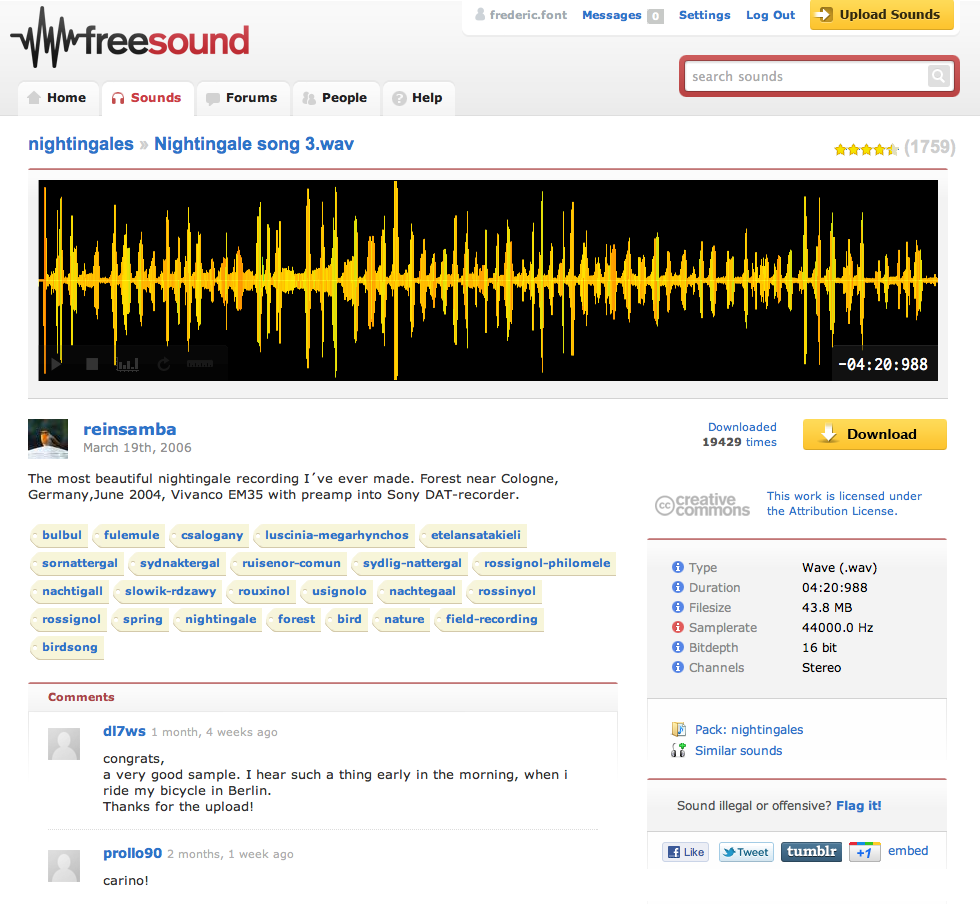
\includegraphics[width=0.8\columnwidth]{ch99/pics/freesound_screenshot.png}}
 \caption{Screenshot of a sound page of Freesound.}
 \label{fig:app:screenshot}
\end{figure}

All the content in Freesound is released under Creative Commons licenses. When uploading sounds, Freesound users can choose between CC0 (public domain), Attribution and Attri\-bu\-tion-NonCommercial licences\footnote{\url{http://www.creativecommons.org/licenses}}. The reason to offer these licenses is to ensure that all the content uploaded in Freesound can be reused by other users, developers and researchers, but at the same time we provide users the option to require the attribution of their work or to restrict the use of their sounds to non-commercial activities. Furthermore, the source code of the web application is released as open source\footnote{\url{http://www.github.com/MTG/freesound}} under the GNU AGPL license\footnote{\url{http://www.gnu.org/licenses/agpl.html}}.

\begin{figure}
 \centerline{
 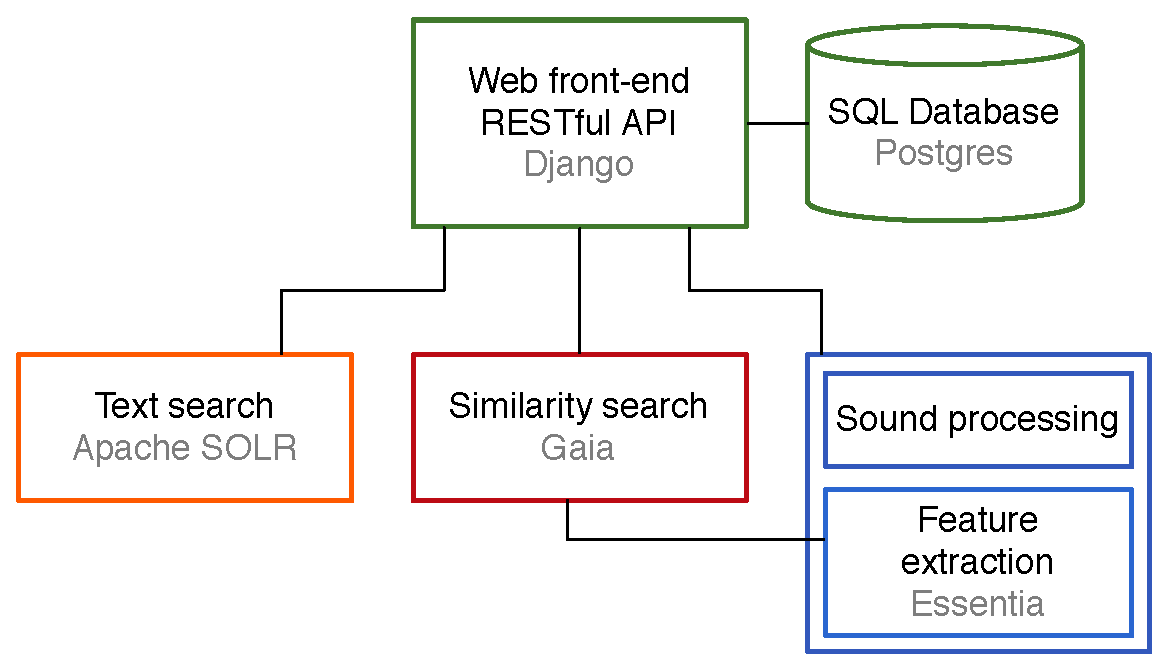
\includegraphics[width=0.7\columnwidth]{ch99/pics/architecture.eps}}
 \caption{Simplified diagram of the Freesound architecture~\citep{Font2013b}.}
 \label{fig:app:architecture}
\end{figure}

Freesound was built with high load and scalability in mind. 
Fig.~\ref{fig:app:architecture} shows a block diagram of its architecture. 
Retrieval of sounds can be performed using text queries, audio content-based similarity search, or by browsing tags or geotags. 
Content-based similarity search is performed over a broad set of low-level audio features\footnote{A list of these features can be found here: \url{http://www.freesound.org/apiv2/descriptors/} (requires Freesound account).}, extracted with Essentia\footnote{\url{http://essentia.upf.edu}}~\citep{Bogdanov2013}, an open-source audio feature extraction tool also developed at the Music Technology Group, and indexed in Gaia\footnote{\url{http://github.com/mtg/gaia}}, another open-source tool developed at the Music Technology Group to build and query large feature spaces.
The front-end is a Django\footnote{\url{http://www.djangoproject.com}} application which includes basic social interaction features (forum, sound comments, sound ratings, private messaging, etc.), and using a PostgreSQL\footnote{\url{http://www.postgresql.org}} database for permanent storage.
Text indexing is supported by an Apache Solr\footnote{\url{http://lucene.apache.org/solr}} server including text descriptions and tags, which allows for sophisticated text queries using the Solr query syntax. 
A distributed architecture is used for processing incoming sounds, producing compressed previews and waveform/spectrogram images, as well as for audio feature extraction. Frame-level and sound-level features are available for each sound.

In 2011, a major update to Freesound was deployed which included a complete redesign of both the backend and the frontend the site, and introduced an API to facilitate access to the Freesound content to researchers and developers\footnote{\url{http://www.freesound.org/docs/api/}}. The API runs as a Django application based on the RESTful principles. 
With the Freesound API users can browse, search, and retrieve information about Freesound users, packs, and the sounds themselves, and also upload, comment, rate and bookmark sounds. 
Furthermore, the API allows to search for similar sounds to a given target (based on audio content features) and to retrieve content features extracted from the audio files, as well as to perform advanced queries combining content analysis features and other metadata such as tags and textual descriptions. 

In the following sections we briefly describe some information about Freeound which can be of interest to the reader of this thesis.
First, we provide statistics about some aspects of general interest. % (Sec.~\ref{sec:app:freeosund_gen_numbers}).
Then, we provide further insight into the community of users around Freesound. % (Sec.~\ref{sec:app:survey}).
For further information we refer the reader to previous publications by the authors~\citep{Font2012,Font,Font2013b}.

\section{General numbers}
\label{sec:app:freeosund_gen_numbers}

\begin{table}
\begin{threeparttable}
\ra{1.2}
\footnotesize
  \begin{center}
    \makebox[0pt]{
    \begin{tabular}{@{}lr@{\hskip 1.0cm}lr@{}} %
      \toprule
      Number of sounds 	& 						230,327  	&  Number of contributor users\tnote{a} & 		14,353  \\
      Number of sound packs &					14,004 	 	&  Number of unique tags\tnote{b} & 			77,753 \\ 
      Number of sound comments & 				191,556 	&  Number of tag applications 	& 				1,670,159	\\
      Number of sound ratings &  				929,380 	&  Average number of tags per sound & 			7.19 	\\ % 5.233 std
      Number of sound downloads & 				65,399,428  &  Number of forum posts & 						47,350 \\  
      Number of registered users & 				4,341,738   &  Number of forum threads & 					9,648 \\
      
      \bottomrule
    \end{tabular}
  }
    \begin{tablenotes}
    \item[a] Users that have contributed by uploading, at least, one sound.
    \item[b] Not necessarily semantically unique.
    \end{tablenotes}
  \caption[Basic statistics of Freesound]{Basic statistics of Freesound (at the time of this writing).}
  \label{app:tab:fs_stats}
  \end{center}
\end{threeparttable}
\end{table}

\begin{figure}
\centerline{\includegraphics[width=1.0\columnwidth]{ch99/pics/Number_of_sounds}}
\caption[Evolution of the number of sounds]{Evolution of the number of uploaded sounds per month. The stronger line corresponds to a smoothed version of the number of uploaded sounds, using a Hann window of 11 points.}
\label{app:fs:new_sounds}
\end{figure}

\begin{figure}
\centerline{\includegraphics[width=1.0\columnwidth]{ch99/pics/Number_of_users}}
\caption[Evolution of the number of newly registered users]{Evolution of the number of newly registered users per month. The stronger line corresponds to a smoothed version of the number of newly registered users, using a Hann window of 11 points.}
\label{app:fs:new_users}
\end{figure}


In Table \ref{app:tab:fs_stats} we report some numbers of general interest about several Freesound aspects such as the number of sounds, users, tags and the distinct social activities.
Figs.~\ref{app:fs:new_sounds},~\ref{app:fs:new_users} and~\ref{app:fs:new_tags} complement these numbers by showing the evolution of the number of uploaded sounds, newly registered users, and new tags per month.
It is particularly interesting to observe that both the number of uploaded sounds and newly registered users per month has been steadily increasing since the start of Freesound in 2005.
Furthermore, it is interesting to note the sudden increase in the number of new tags per month that happened along with the aforementioned redesign of Freesound (Sec.~~\ref{appendix:Freesound_intro}) and the later decrease after the introduction of the tag recommendation system (Fig.~\ref{app:fs:new_tags}).
This evolution suggests that the new Freesound design had a huge impact on the way users annotate sounds, resulting in less reuse of tags. This might be explained because, before the redesign, Freesound's annotation interface included a section in which the most commonly used tags by someone annotating a sound were shown. This section was removed after the redesign.
After the introduction of tag recommendation however, the rate at which new tags are created diminishes, as we already observed and discussed in Chapter~\ref{sec:impact} (Sec.~\ref{impact:sec:percentage_of_new_tags_results}) and can also be seen in Fig.~\ref{app:fs:new_tags}.


\begin{figure}
\centerline{\includegraphics[width=1.0\columnwidth]{ch99/pics/Number_of_new_tags}}
\caption[Evolution of the number of new tags]{Evolution of the number of new tags per month. The stronger line corresponds to a smoothed version of the number of new tags, using a Hann window of 11 points.}
\label{app:fs:new_tags}
\end{figure}


%\begin{figure}
%\centerline{\includegraphics[width=\figSizeMidLarge]{ch99/pics/Number_of_tag_applications}}
%\caption[Evolution of the number of new tag applications]{Evolution of the number of new tag applications per month. The stronger line corresponds to a smoothed version of the number of new tag applications, using a Hann window of 11 points.}
%\label{app:fs:new_tag_applications}
%\end{figure}


\section{Freesound's community of users}
\label{sec:app:survey}

%The active contributors in the community have played an important role in the development of the platform, since quite a number of the software improvements have been the result of suggestions from the community or have been discussed within it. Two basic goals have driven most of the development of Freesound: quality and quantity of sounds. We wanted to gather as many user contributed sounds as possible, but not at any price. Sounds have to be of good quality and have to be well described in order to be easily found and reused.

The active community of users behind Freesound is the clearest indication of its success.
As we have already seen, the community has been growing over time, reaching more than 4 million registered users and 14,000 unique sound contributors at the time of this writing.
Freesound's community can be characterised as a ``task-oriented'' community, that is to say, a community where its members pursue some collective goals that benefit the whole community~\citep{Stanoevska-slabeva2002a}. 
To get some insight in that aspect, we carried out a small online survey in the Freesound forums, asking users about their opinion on the existence of shared goals and, if so, which are these goals.
A total of 86 Freesound users participated in the survey, 50 of them agreeing with the existence of shared goals, and the others either not directly answering the question (31) or denying the existence of these goals (5).
Shared goals that users described in their responses are quite diverse. However, the most repeated goals could be summarized as ``sharing sounds'' (mentioned by 43\% of those participants agreeing with the existence of shared goals), ``building a big sound archive'' (30\%) and ``helping each other by uploading useful sounds'' (21\%).

Furthermore, in that same survey we also asked users about the things that make Freesound different from other similar sites. In that case, 66\% of users pointed either at the quantity, quality, diversity or ``freeness'' of accessible sounds, all of them being primary design criteria for Freesound. Other common answers are related to the user interface or the focus on sharing sound samples rather than music (24\% of the responses). 

Finally, we asked users about the applications for which Freesound is being used (i.e.,~for what purposes Freesound samples are being reused). 
Responses show that the most important usage of Freesound samples is in movies and animations (35\%), followed by music (20\%), theatre (9\%), sound design (9\%), education and academy (6\%), and videogames (5\%). Particularly interesting is the fact that the remaining 16\% of users pointed out Freesound itself as an application, and hence mainly using Freesound for listening, sharing and contributing sounds, and for its basic social functionalities.
 
\cleartorecto%!TEX root = ../thesis_a4.tex

\chapter{Appendix B: publications by the author}
\label{sec:Pubs}


\section*{In press}

Font, F., Serr\`a, J., \& Serra, X. (2015). Analysis of the impact of a tag rec-
ommendation system in a real-world folksonomy. \emph{ACM Transactions on Intelligent Systems and Technology.}



\section*{Journal papers}


Font, F., Serr\`a, J., \& Serra, X. (2014c). Class-based tag recommendation and user-based evaluation in online audio clip sharing. \emph{Knowledge Based Systems, 67}, 131--142.

\vspace{0.2cm}

Font, F., Serr\`a, J., \& Serra, X. (2013). Folksonomy-based tag recommendation for collaborative tagging systems. \emph{International Journal on Semantic Web and Information Systems, 9}(2), 1--30.

\vspace{0.2cm}

Roma, G., Herrera, P., Zanin, M., Toral, S.L., Font, F., \& Serra, X. (2012) Small world networks and creativity in audio clip sharing. \emph{Journal of Social Network Mining, 1}(1), 112--127.


\section*{Conference papers}

Font, F., Oramas, S., Fazekas, G., \& Serra, X. (2014a). Extending Tagging Ontologies with Domain Specific Knowledge. In \emph{Proceedings of the International Semantic Web Conference (ISWC, Poster track)}.

\vspace{0.2cm}

Font, F., Serr\`a, J., \& Serra, X. (2014b). Audio clip classification using social tags and the effect of tag expansion. In \emph{Proceedings of the AES Conference on Semantic Audio}.

\vspace{0.2cm}

Font, F., Roma G., \& Serra, X. (2013).  Freesound Technical Demo. In \emph{Proceedings of the ACM International Conference on Multimedia (MM)}, pp. 411–-412.

\vspace{0.2cm}

Font, F., Serr\`a, J., \& Serra, X. (2012). Folksonomy-based tag recommendation for online audio clip sharing. In \emph{Proceedings of the International Conference on Music Information Retrieval (ISMIR 2012)}, pp. 73–-78.

\vspace{0.2cm}

Font, F., \& Serra, X. (2012).  Analysis of the Folksonomy of Freesound. \emph{Proceedings of the CompMusic Workshop}, pp. 48--54.

\vspace{0.2cm}

Font, F., Roma G., Herrera P., \& Serra, X. (2012).  Characterization of the Freesound Online Community. In \emph{Proceedings of the International Workshop on Cognitive Information Processing (CIP)}, pp. 279--284.

\vspace{0.2cm}

Font, F., \& Serra, X. (2011).  Extending Sound Sample Descriptions through the Extraction of Community Knowledge. In \emph{Proceedings of the International Conference on User Modeling, Adaptation and Personalization (UMAP)}, pp. 418--421.

\vspace{0.2cm}

Akkermans, V., Font F., Funollet J., De Jong, B, Roma G., Togias S., \& Serra, X. (2011).  Freesound 2: An Improved Platform for Sharing Audio Clips. Demo session at the \emph{International Conference on Music Information Retrieval (ISMIR)}.
%\cleartorecto\include{ch99/quotation}
\cleartorecto\newpage\thispagestyle{empty}\mbox{}

\end{document}

%------------------------------------------------------------------------------------------------
% -----------------------------------------------------------------------------------------------
%------------------------------------------------------------------------------------------------
%------------------------------------------------------------------------------------------------
